\documentclass[10]{article}


\usepackage{hyperref}
\usepackage{amsfonts,amssymb,amsmath,amsthm,cite}
\usepackage{graphicx}
\usepackage[toc,page]{appendix}
\usepackage{nicefrac}
%% \usepackage[francais]{babel}
\usepackage[applemac]{inputenc}
\usepackage{amssymb, euscript}
\usepackage[matrix,arrow,curve]{xy}
\usepackage{graphicx}
\usepackage{tabularx}
\usepackage{float}
\usepackage{tikz}
\usepackage{slashed}
\usepackage{mathrsfs}
\usepackage{multirow}
\usepackage{rotating}
\usepackage{mathbbol}

%\usepackage{mathtools}

\usetikzlibrary{matrix}
\usetikzlibrary{cd}

\usepackage{siunitx}

\usepackage{lmodern}
\usepackage[T1]{fontenc}
\usepackage[babel=true]{microtype}


\usepackage{amsfonts,cite}
\usepackage{graphicx}

%% \usepackage[francais]{babel}
\usepackage[applemac]{inputenc}


\usepackage[sc]{mathpazo}
\usepackage{environ}

\linespread{1.05}         % Palatino needs more leading (space between lines)


%\usepackage[usenames]{color}



\DeclareFontFamily{T1}{pzc}{}
\DeclareFontShape{T1}{pzc}{m}{it}{1.8 <-> pzcmi8t}{}
\DeclareMathAlphabet{\mathpzc}{T1}{pzc}{m}{it}
% the command for it is \mathpzc

\textwidth=140mm


% % % % % % % % % % % % % % % % % % % %
\theoremstyle{plain}
\newtheorem{prop}{Proposition}[section]
\newtheorem{prdf}[prop]{Proposition and Definition}
\newtheorem{lem}[prop]{Lemma}%[section]
\newtheorem{cor}[prop]{Corollary}%[section]
\newtheorem{thm}[prop]{Theorem}%[section]
\newtheorem{theorem}[prop]{Theorem}
\newtheorem{lemma}[prop]{Lemma}
\newtheorem{proposition}[prop]{Proposition}
\newtheorem{corollary}[prop]{Corollary}
\newtheorem{statement}[prop]{Statement}

\theoremstyle{definition}
\newtheorem{defn}[prop]{Definition}%[section]
\newtheorem{cordefn}[prop]{Corollary and Definition}%[section]
\newtheorem{empt}[prop]{}%[section]
\newtheorem{exm}[prop]{Example}%[section]
\newtheorem{rem}[prop]{Remark}%[section]
\newtheorem{prob}[prop]{Problem}
\newtheorem{conj}{Conjecture}       %% Hypothesis 1
\newtheorem{cond}{Condition}        %% Condition 1
%\newtheorem{axiom}[thm]{Axiom}           %% Axiom 1 modified
\newtheorem{fact}[prop]{Fact}
\newtheorem{ques}{Question}         %% Question 1
\newtheorem{answ}{Answer}           %% Answer 1
\newtheorem{notn}{Notation}        %% Notations are not numbered

\theoremstyle{definition}
\newtheorem{notation}[prop]{Notation}
\newtheorem{definition}[prop]{Definition}
\newtheorem{example}[prop]{Example}
\newtheorem{exercise}[prop]{Exercise}
\newtheorem{conclusion}[prop]{Conclusion}
\newtheorem{conjecture}[prop]{Conjecture}
\newtheorem{criterion}[prop]{Criterion}
\newtheorem{summary}[prop]{Summary}
\newtheorem{axiom}[prop]{Axiom}
\newtheorem{problem}[prop]{Problem}
%\theoremstyle{remark}
\newtheorem{remark}[prop]{Remark}

\numberwithin{equation}{section}
\newtheorem*{claim}{Claim}
\DeclareMathOperator{\Dom}{Dom}              %% domain of an operator
\newcommand{\Dslash}{{D\mkern-11.5mu/\,}}    %% Dirac operator
\newcommand{\trG}{{\rm tr}_G\;}
\newcommand{\trF}{{\rm tr}_{\mathcal F}\;}
\newcommand{\TR}{{\rm TR}\;}
\newcommand{\res}{{\rm res}\;}


\newcommand\ci{${\mathcal C}^{\infty}$}
\newcommand\CI{{\mathcal C}^{\infty}}
\newcommand\CIc{{\mathcal C}^{\infty}_{\text{c}}}

%\newcommand\myeq{\stackrel{\mathclap{\normalfont\mbox{def}}}{=}}
\newcommand{\rar}[1]{\stackrel{#1}{\longrightarrow}}
\newcommand{\lar}[1]{\stackrel{#1}{\longleftarrow}}

\newcommand{\nor}[1]{\left\Vert #1\right\Vert}    %\nor{x}=||x||
\newcommand{\norm}[1]{\left\| #1\right\|}    %\nor{x}=||x||
\newcommand{\vertiii}[1]{{\left\vert\kern-0.25ex\left\vert\kern-0.25ex\left\vert #1
		\right\vert\kern-0.25ex\right\vert\kern-0.25ex\right\vert}}
\newcommand{\Ga}{\Gamma}  
\newcommand{\Cker}{\mathrm{coker}}                   %% short for  \Gamma
\newcommand{\Coo}{C^\infty}                  %% smooth functions
\newcommand{\dom}{\mathrm{dom}}                  %% smooth functions
\newcommand{\Cont}{C} 
\newcommand{\cl}{\overline} 
\newcommand{\Contc}{C_c} 
\newcommand{\Contb}{C_b} 
\newcommand{\Repi}{\mathrm{Rep}_{int}} 
\newcommand{\Rep}{\mathrm{Rep}} 
\newcommand{\hor}[0]{\mathrm{hor}}
\newcommand{\Cmp}{\operatorname{comp}}
\newcommand{\adb}{\operatorname{adb}}
\newcommand{\dist}{\operatorname{dist}}
 \newcommand{\onto}{\to\mkern-14mu\to}

% % % % % % % % % % % % % % % % % % % %


\usepackage[sc]{mathpazo}
\linespread{1.05}         % Palatino needs more leading (space between lines)

\newbox\ncintdbox \newbox\ncinttbox %% noncommutative integral symbols
\setbox0=\hbox{$-$} \setbox2=\hbox{$\displaystyle\int$}
\setbox\ncintdbox=\hbox{\rlap{\hbox
		to \wd2{\hskip-.125em \box2\relax\hfil}}\box0\kern.1em}
\setbox0=\hbox{$\vcenter{\hrule width 4pt}$}
\setbox2=\hbox{$\textstyle\int$} \setbox\ncinttbox=\hbox{\rlap{\hbox
		to \wd2{\hskip-.175em \box2\relax\hfil}}\box0\kern.1em}

\newcommand{\ncint}{\mathop{\mathchoice{\Cpy\ncintdbox}%
		{\Cpy\ncinttbox}{\Cpy\ncinttbox}%
		{\Cpy\ncinttbox}}\nolimits}  %% NC integral

%%% Repeated relations:
\newcommand{\xyx}{\times\cdots\times}      %% repeated product
\newcommand{\opyop}{\oplus\cdots\oplus}    %% repeated direct sum
\newcommand{\oxyox}{\otimes\cdots\otimes}  %% repeated tensor product
\newcommand{\wyw}{\wedge\cdots\wedge}      %% repeated exterior product
\newcommand{\subysub}{\subset\hdots\subset}      %% repeated subset
\newcommand{\supysup}{\supset\hdots\supset}      %% repeated supset
\newcommand\CC{\mathbb C}
\newcommand\NN{\mathbb N}
\newcommand\RR{\mathbb R}
\newcommand\ZZ{\mathbb Z}
\newcommand{\LGR}{\matcal L}
\newcommand{\rep}{\mathfrak{rep}}
\newcommand{\lift}{\mathfrak{lift}}
\newcommand{\desc}{\mathfrak{desc}}
\newcommand{\Cstar}{C^*}
\newcommand{\Cst}{C^*}
\newcommand{\AN}{\mathcal{A}_N} 
\newcommand{\Gh}{\Gamma_{\mathrm{hol}}} 
\newcommand{\Star}{*}
\newcommand{\PS}[1]{\Psi^{#1}(\GR;E)}
\newcommand{\opi}{1P\fchoice{\kern .08em}{}I}


%%% Roman letters:
\newcommand{\id}{\mathrm{id}}                %% identity map
\newcommand{\Id}{\mathrm{Id}}                %% identity map
\newcommand{\pt}{\mathrm{pt ???}}                %% a point
\newcommand{\Cnst}{\mathrm{const}}          %% a constant
\newcommand{\Cdim}{\mathrm{codim}}          %% codimension
\newcommand{\cyc}{\mathrm{cyclic}}  %% cyclic sum
\renewcommand{\d}{\mathrm{d}}       %% commutative differential
\newcommand{\dR}{\mathrm{dR}}       %% de~Rham cohomology
\newcommand{\proj}{\mathrm{proj}}                %% a projection
\newcommand*{\braket}[2]{\langle#1 {,~} #2\rangle}% right inner products
\newcommand*{\lbraket}[2]{\langle\!\langle#1{\mid}#2\rangle\!\rangle}% left inner products

\newcommand*{\Mult}{\mathcal M}% multiplier algebra
\newcommand{\Lt}{\mathcal{L}}                 %%\newcommand{\unitsv}[1]{#1^{(0)}}

\newcommand{\A}{\mathcal{A}}                 %%\newcommand{\unitsv}[1]{#1^{(0)}}
\newcommand{\units}{G^{(0)}}
\newcommand{\haars}{\{\lambda^{u}\}_{u\in\units}}
\newcommand{\shaars}{\{\lambda_{u}\}_{u\in\units}}
\newcommand{\haarsv}[2]{\{\lambda^{#2}_{#1}\}_{#2\in\unitsv{#1}}}
\newcommand{\haarv}[2]{\lambda^{#2}_{#1}}

\renewcommand{\a}{\alpha}                    %% short for  \alphapha
\DeclareMathOperator{\ad}{ad}                %% infml adjoint repn
\newcommand{\as}{\quad\mbox{as}\enspace}     %% `as' with spacing
\newcommand{\Aun}{\widetilde{\mathcal{A}}}   %% unital algebra
\newcommand{\B}{\mathcal{B}}                 %% space of distributions
\newcommand{\E}{\mathcal{E}}                 %% space of distributions
\renewcommand{\b}{\beta}                     %% short for \beta
\newcommand{\braCket}[3]{\langle#1\mathbin|#2\mathbin|#3\rangle}
%\newcommand{\braket}[2]{\langle#1\mathbin|#2\rangle} %% <w|z>
\newcommand{\C}{\mathbb{C}}                  %% complex numbers
\newcommand{\Af}{\mathfrak{A}}
\newcommand{\cc}{\mathbf{c}}                 %% Hochschild cycle
\DeclareMathOperator{\Cl}{C\ell}             %% Clifford algebra
\newcommand{\F}{\mathcal{F}}                 %% space of test functions
\newcommand{\G}{\mathcal{G}}                 %% 
\newcommand{\GR}{\mathcal{G}}                 %% 
\newcommand{\D}{\mathcal{D}}                 %% Moyal L^2-filtration
\renewcommand{\H}{\mathcal{H}}               %% Hilbert space
\newcommand{\half}{\tfrac{1}{2}}             %% small fraction  1/2
\newcommand{\hh}{\mathcal{H}}                %% Hilbert space
\newcommand{\hookto}{\hookrightarrow}        %% abbreviation
\newcommand{\Ht}{{\widetilde{\mathcal{H}}}}  %% Hilbert space of forms
\newcommand{\I}{\mathcal{I}}                 %% tracelike functions
\DeclareMathOperator{\Junk}{Junk}            %% the junk DGA ideal
\newcommand{\K}{\mathcal{K}}                 %% compact operators
\newcommand{\ket}[1]{|#1\rangle}             %% ket vector
\newcommand{\ketbra}[2]{|#1\rangle\langle#2|} %% rank one operator
\renewcommand{\L}{\mathcal{L}}               %% operator algebra
\newcommand{\La}{\Lambda}                    %% short for \Lambda
\newcommand{\la}{\lambda}                    %% short for \lambda
\newcommand{\lf}{L_f^\theta}                 %% left  mult operator
\newcommand{\M}{\mathcal{M}}                 %% Moyal multplr algebra
\newcommand{\Lb}{\mathcal{L}}                 %% Moyal multplr algebra
\newcommand{\mm}{\mathcal{M}^\theta}
%\newcommand{{{\star_{\theta}}}{{\mathchoice{\mathbin{\;|\;ar_{_\theta}}}
			%            {\mathbin{\;|\;ar_{_\theta}}}           %% Moyal
			%            {{\;|\;ar_\theta}}{{\;|\;ar_\theta}}}}    %% product
	\newcommand{\N}{\mathbb{N}}                  %%  integers
	\newcommand{\nb}{\nabla}                     %% gradient
	\newcommand{\Oh}{\mathcal{O}}                %% comm multiplier alg
	\newcommand{\om}{\omega}                     %% short for \omega
	\newcommand{\opp}{{\mathrm{op}}}             %% opposite algebra
	\newcommand{\ox}{\otimes}                    %% tensor product
	\newcommand{\eps}{\varepsilon}                    %% tensor product
	\newcommand{\otimesyox}{\otimes\cdots\otimes}    %% repeated tensor product
	\newcommand{\pa}{\partial}                   %% short for \partial
	\newcommand{\pd}[2]{\frac{\partial#1}{\partial#2}}%% partial derivative
	\newcommand{\piso}[1]{\lfloor#1\rfloor}      %% integer part
	\newcommand{\PsiDO}{\Psi~\mathrm{DO}}         %% pseudodiffl operators
	\newcommand{\Q}{\mathbb{Q}}                  %% rational numbers
	\newcommand{\R}{\mathbb{R}}                  %% real numbers
	\newcommand{\rdl}{R_\Dslash(\lambda)}        %% resolvent
	\newcommand{\roundbraket}[2]{(#1\mathbin|#2)} %% (w|z)
	\newcommand{\row}[3]{{#1}_{#2},\dots,{#1}_{#3}} %% list: a_1,...,a_n
	\newcommand{\sepword}[1]{\quad\mbox{#1}\quad} %% well-spaced words
	\newcommand{\set}[1]{\{\,#1\,\}}             %% set notation
	\newcommand{\Sf}{\mathbb{S}}                 %% sphere
	\newcommand{\uhor}[1]{\Omega^1_{hor}#1}
	\newcommand{\sco}[1]{{\sp{(#1)}}}
	\newcommand{\sw}[1]{{\sb{(#1)}}}
	\DeclareMathOperator{\spec}{sp}              %% spectrum
	\renewcommand{\SS}{\mathcal{S}}              %% Schwartz space
	\newcommand{\sss}{\mathcal{S}}               %% Schwartz space
	\DeclareMathOperator{\supp}{\mathfrak{supp}}            %% support
	\newcommand{\T}{\mathbb{T}}                  %% circle as a group
	\renewcommand{\th}{\theta}                   %% short for \theta
	\newcommand{\thalf}{\tfrac{1}{2}}            %% small* fraction 1/2
	\newcommand{\tihalf}{\tfrac{i}{2}}           %% small* fraction i/2
	\newcommand{\tpi}{{\tilde\pi}}               %% extended representation
	\DeclareMathOperator{\Tr}{Tr}                %% trace of operator
	\DeclareMathOperator{\tr}{tr}                %% trace of matrix
	\newcommand{\del}{\partial}                  %% short for  \partial
	\DeclareMathOperator{\tsum}{{\textstyle\sum}} %% small sum in display
	\newcommand{\V}{\mathcal{V}}                 %% test function space
	\newcommand{\vac}{\ket{0}}                   %% vacuum ket vector
	\newcommand{\vf}{\varphi}                    %% scalar field
	\newcommand{\w}{\wedge}                      %% exterior product
	\DeclareMathOperator{\wres}{wres}            %% density of Wresidue
	\newcommand{\x}{\times}                      %% cross
	\newcommand{\Z}{\mathbb{Z}}                  %% integers
	\newcommand{\7}{\dagger}                     %% short for + symbol
	\newcommand{\8}{\bullet}                     %% anonymous degree
	\renewcommand{\.}{\cdot}                     %% anonymous variable
	\renewcommand{\:}{:}                    %% colon in  f: A -> B
	
	
	%\newcommand{\sA}{\mathscr{A}}       %%
	\newcommand{\Nhat}{\hat{\mathbb{N}}} 
	\newcommand{\sA}{\mathcal{A}} 
	\newcommand{\sB}{\mathcal{B}}       %%
	\newcommand{\sC}{\mathcal{C}}       %%
	\newcommand{\sD}{\mathcal{D}}       %%
	\newcommand{\sE}{\mathcal{E}}       %%
	\newcommand{\sF}{\mathcal{F}}       %%
	\newcommand{\sG}{\mathcal{G}}       %%
	\newcommand{\sH}{\mathcal{H}}       %%
	\newcommand{\sI}{\mathcal{I}}       %%
	\newcommand{\sJ}{\mathcal{J}}       %%
	\newcommand{\sK}{\mathcal{K}}       %%
	\newcommand{\sL}{\mathcal{L}}       %%
	\newcommand{\sM}{\mathcal{M}}       %%
	\newcommand{\sN}{\mathcal{N}}       %%
	\newcommand{\sO}{\mathcal{O}}       %%
	\newcommand{\sP}{\mathcal{P}}       %%
	\newcommand{\sQ}{\mathcal{Q}}       %%
	\newcommand{\sR}{\mathcal{R}}       %%
	\newcommand{\sS}{\mathcal{S}}       %%
	\newcommand{\sT}{\mathcal{T}}       %%
	\newcommand{\sU}{\mathcal{U}}       %%
	\newcommand{\sV}{\mathcal{V}}       %%
	\newcommand{\sX}{\mathcal{X}}       %%
	\newcommand{\sY}{\mathcal{Y}}       %%
	\newcommand{\sZ}{\mathcal{Z}}       %%
	
	\newcommand{\Om}{\Omega}       %%
	
	
	\DeclareMathOperator{\ptr}{ptr}     %% Poisson trace
	\DeclareMathOperator{\Trw}{Tr_\omega} %% Dixmier trace
	\DeclareMathOperator{\vol}{Vol}     %% total volume
	\DeclareMathOperator{\Vol}{Vol}     %% total volume
	\DeclareMathOperator{\Area}{Area}   %% area of a surface
	\DeclareMathOperator{\Wres}{Wres}   %% (Wodzicki) residue
	
	\newcommand{\dd}[1]{\frac{\partial}{\partial#1}}   %% partial derivation
	\newcommand{\ddt}[1]{\frac{d}{d#1}}                %% derivative
	\newcommand{\inv}[1]{\frac{1}{#1}}                 %% inverse
	\newcommand{\sfrac}[2]{{\scriptstyle\frac{#1}{#2}}} %% tiny fraction
	
	\newcommand\VD{{\mathcal D}}
	\newcommand{\bA}{\mathbb{A}}       %%
	\newcommand{\bB}{\mathbb{B}}       %%
	\newcommand{\bC}{\mathbb{C}}       %%
	\newcommand{\bCP}{\mathbb{C}P}     %%
	\newcommand{\bD}{\mathbb{D}}       %%
	\newcommand{\bE}{\mathbb{E}}       %%
	\newcommand{\bF}{\mathbb{F}}       %%
	\newcommand{\bG}{\mathbb{G}}       %%
	\newcommand{\bH}{\mathbb{H}}       %%
	\newcommand{\bHP}{\mathbb{H}P}     %%
	\newcommand{\bI}{\mathbb{I}}       %%
	\newcommand{\bJ}{\mathbb{J}}       %%
	\newcommand{\bK}{\mathbb{K}}       %%
	\newcommand{\bL}{\mathbb{L}}       %%
	\newcommand{\bM}{\mathbb{M}}       %%
	\newcommand{\bN}{\mathbb{N}}       %%
	\newcommand{\bO}{\mathbb{O}}       %%
	\newcommand{\bOP}{\mathbb{O}P}     %%
	\newcommand{\bP}{\mathbb{P}}       %%
	\newcommand{\bQ}{\mathbb{Q}}       %%
	\newcommand{\bR}{\mathbb{R}}       %%
	\newcommand{\bRP}{\mathbb{R}P}     %%
	\newcommand{\bS}{\mathbb{S}}       %%
	\newcommand{\bT}{\mathbb{T}}       %%
	\newcommand{\bU}{\mathbb{U}}       %%
	\newcommand{\bV}{\mathbb{V}}       %%
	\newcommand{\bX}{\mathbb{X}}       %%
	\newcommand{\bY}{\mathbb{Y}}       %%
	\newcommand{\bZ}{\mathbb{Z}}       %%
	
	\newcommand{\bydef}{\stackrel{\mathrm{def}}{=}}          %% 
	\newcommand{\defeq}{\stackrel{\mathrm{def}}{=}}
	\newcommand{\ntr}{\widetilde{\smash\tr\vphantom{\raise.5pt\hbox{r}}}}
	   
	
	
	
	\newcommand{\al}{\alpha}          %% short for  \alpha
	\newcommand{\bt}{\beta}           %% short for  \beta
	\newcommand{\Dl}{\Delta}          %% short for  \Delta
	\newcommand{\dl}{\delta}          %% short for  \delta
	\newcommand{\ga}{\gamma}          %% short for  \gamma
	\newcommand{\ka}{\kappa}          %% short for  \kappa
	\newcommand{\sg}{\sigma}          %% short for  \sigma
	\newcommand{\Sg}{\Sigma}          %% short for  \Sigma
	\newcommand{\Th}{\Theta}          %% short for  \Theta
	\renewcommand{\th}{\theta}        %% short for  \theta
	\newcommand{\vth}{\vartheta}      %% short for  \vartheta
	\newcommand{\ze}{\zeta}           %% short for  \zeta
	
	\DeclareMathOperator{\ord}{ord}     %% order of a PsiDO
	\DeclareMathOperator{\rank}{rank}   %% rank of a vector bundle
	\DeclareMathOperator{\sign}{sign}   %%
	\DeclareMathOperator{\sgn}{sgn}   %%
	\DeclareMathOperator{\chr}{char}   %%
	\DeclareMathOperator{\ev}{ev}       %% evaluation
	\newcommand{\Or}{\mathcal{O}}
	
	\newcommand{\Op}{\mathbf{Op}}
	\newcommand{\As}{\mathbf{As}}
	\newcommand{\Com}{\mathbf{Com}}
	\newcommand{\LLie}{\mathbf{Lie}}
	\newcommand{\Leib}{\mathbf{Leib}}
	\newcommand{\Zinb}{\mathbf{Zinb}}
	\newcommand{\Poiss}{\mathbf{Poiss}}
	
	\newcommand{\gX}{\mathfrak{X}}      %% vector fields
	\newcommand{\sol}{\mathfrak{so}}    %% special orthogonal Lie algebra
	\newcommand{\gm}{\mathfrak{m}}      %% maximal ideal
	
	
	\DeclareMathOperator{\Res}{Res}
	\DeclareMathOperator{\NCRes}{NCRes}
	\DeclareMathOperator{\Ind}{Ind}
	%% co/homology theories
	\DeclareMathOperator{\rH}{H}        %% any co/homology
	\DeclareMathOperator{\rC}{C}        %%  any co/chains
	\DeclareMathOperator{\rZ}{Z}        %% cycles
	\DeclareMathOperator{\rB}{B}        %% boundaries
	\DeclareMathOperator{\rF}{F}        %% filtration
	\DeclareMathOperator{\Gr}{gr}        %% associated graded object
	\DeclareMathOperator{\rHc}{H_{\mathrm{c}}}   %% co/homology with compact support
	\DeclareMathOperator{\drH}{H_{\mathrm{dR}}}  %% de Rham co/homology
	\DeclareMathOperator{\cechH}{\check{H}}    %% Cech co/homology
	\DeclareMathOperator{\rK}{K}        %% K-groups
	\DeclareMathOperator{\rKO}{KO}        %% real K-groups
	\DeclareMathOperator{\rKU}{KU}        %% unitary K-groups
	\DeclareMathOperator{\rKSp}{KSp}        %% symplectic K-groups
	\DeclareMathOperator{\rR}{R}        %% representation ring
	\DeclareMathOperator{\rI}{I}        %% augmentation ideal
	\DeclareMathOperator{\HH}{HH}       %% Hochschild co/homology
	\DeclareMathOperator{\HC}{HC}       %% cyclic co/homology
	\DeclareMathOperator{\HP}{HP}       %% periodic cyclic co/homology
	\DeclareMathOperator{\HN}{HN}       %% negative cyclic co/homology
	\DeclareMathOperator{\HL}{HL}       %% Leibniz co/homology
	\DeclareMathOperator{\KK}{KK}       %% KK-theory
	\DeclareMathOperator{\KKK}{\mathbf{KK}}       %% KK-theory as a category
	\DeclareMathOperator{\Ell}{Ell}       %% Abstract elliptic operators
	\DeclareMathOperator{\cd}{cd}       %% cohomological dimension
	\DeclareMathOperator{\spn}{span}       %% span
	\DeclareMathOperator{\linspan}{span} %% linear span (can't use \span)
	\newcommand{\blank}{-}   
	
	
	
	\newcommand{\twobytwo}[4]{\begin{pmatrix} #1 & #2 \\ #3 & #4 \end{pmatrix}}
	\newcommand{\CGq}[6]{C_q\!\begin{pmatrix}#1&#2&#3\\#4&#5&#6\end{pmatrix}}
	%% q-Clebsch--Gordan coefficients
	\newcommand{\cz}{{\bullet}}         %% anonymous degree
	\newcommand{\nic}{{\vphantom{\dagger}}} %% invisible dagger
	\newcommand{\ep}{{\dagger}}         %% abbreviation for + symbol
	\newcommand{\downto}{\downarrow}    %% right hand limit
	\newcommand{\isom}{\in}          %% isomorphism
	\newcommand{\lt}{\triangleright}    %% a left  action
	\newcommand{\otto}{\leftrightarrow} %% bijection
	\newcommand{\rt}{\triangleleft}     %% a right action
	\newcommand{\semi}{\rtimes}         %% crossed product
	\newcommand{\tensor}{\otimes}       %% tensor product
	\newcommand{\Ctensor}{\square}       %% cotensor product
	\newcommand{\trans}{\pitchfork}     %% transverse
	\newcommand{\ul}{\underline}        %% for sheaves
	\newcommand{\upto}{\uparrow}        %% left  hand limit
	\renewcommand{\:}{:}           %% colon in  f: A -> B
	\newcommand{\blt}{\ast}
	\newcommand{\Co}{C_{\bullet}}
	\newcommand{\cCo}{C^{\bullet}}
	\newcommand{\nbs}{\nabla^S}         %% spin connection
	\newcommand{\up}{{\mathord{\uparrow}}} %% `up' spinors
	\newcommand{\dn}{{\mathord{\downarrow}}} %% `down' spinors
	\newcommand{\updn}{{\mathord{\updownarrow}}} %% up or down
	
	%%% Bilinear enclosures:
	
	\newcommand{\bbraket}[2]{\langle\!\langle#1\stroke#2\rangle\!\rangle}
	%% <<w|z>>
	\newcommand{\bracket}[2]{\langle#1,\, #2\rangle} %% <w,z>
	\newcommand{\scalar}[2]{\langle#1,\,#2\rangle} %% <w,z>
	\newcommand{\poiss}[2]{\{#1,\,#2\}} %% {w,z}
	\newcommand{\dst}[2]{\langle#1,#2\rangle} %% distributions <u,\phi>
	\newcommand{\pairing}[2]{(#1\stroke #2)} %% right-linear pairing
	\def\<#1|#2>{\langle#1\stroke#2\rangle} %% \braket (Dirac notation)
	\def\?#1|#2?{\{#1\stroke#2\}}        %% left-linear pairing
	
	%%% Accent-like macros:
	
	\renewcommand{\Bar}[1]{\overline{#1}} %% closure operator
	\renewcommand{\Hat}[1]{\widehat{#1}}  %% short for \widehat
	\renewcommand{\Tilde}[1]{\widetilde{#1}} %% short for \widetilde
	
	
	\DeclareMathOperator{\bCl}{\bC l}   %% complex Clifford algebra
	
	%%% Small fractions in displays:
	
	\newcommand{\ihalf}{\tfrac{i}{2}}   %% small fraction  i/2
	\newcommand{\quarter}{\tfrac{1}{4}} %% small fraction  1/4
	\newcommand{\shalf}{{\scriptstyle\frac{1}{2}}}  %% tiny fraction  1/2
	\newcommand{\third}{\tfrac{1}{3}}   %% small fraction  1/3
	\newcommand{\ssesq}{{\scriptstyle\frac{3}{2}}} %% tiny fraction  3/2
	\newcommand{\sesq}{{\mathchoice{\tsesq}{\tsesq}{\ssesq}{\ssesq}}} %% 3/2
	\newcommand{\tsesq}{\tfrac{3}{2}}   %% small fraction  3/2
	
	
	%\newcommand\eqdef{\over set{\mathclap{\normalfont\mbox{def}}}{=}}
	\newcommand\eqdef{\over set{\mathrm{def}}{=}}
	
	
	%+++++++++++++++++++++++++++++++++++
	
	\newcommand{\word}[1]{\quad\text{#1}\enspace} %% well-spaced words
	\newcommand{\words}[1]{\quad\text{#1}\quad} %% better-spaced words
	\newcommand{\su}[1]{{\sp{[#1]}}}
	
	\def\<#1,#2>{\langle#1,#2\rangle}            %% bilinear pairing
	\def\ee_#1{e_{{\scriptscriptstyle#1}}}       %% basis projector
	\def\wick:#1:{\mathopen:#1\mathclose:}       %% Wick-ordered operator
	
	\newcommand{\opname}[1]{\mathop{\mathrm{#1}}\nolimits}
	
	\newcommand{\hideqed}{\renewcommand{\qed}{}} %% to suppress `\qed'
	
	
	%%%%%%%%%%%%%%%%%%%%%%%%%%%%%
	%% 2. Some internal machinery
	%%%%%%%%%%%%%%%%%%%%%%%%%%%%%
	
	\newbox\ncintdbox \newbox\ncinttbox %% noncommutative integral symbols
	\setbox0=\hbox{$-$}
	\setbox2=\hbox{$\displaystyle\int$}
	\setbox\ncintdbox=\hbox{\rlap{\hbox
			to \wd2{\box2\relax\hfil}}\box0\kern.1em}
	\setbox0=\hbox{$\vcenter{\hrule width 4pt}$}
	\setbox2=\hbox{$\textstyle\int$}
	\setbox\ncinttbox=\hbox{\rlap{\hbox
			to \wd2{\hskip-.05em\box2\relax\hfil}}\box0\kern.1em}
	
	\newcommand{\disp}{\displaystyle} %% short for  \displaystyle
	
	%\newcommand{\hideqed}{\renewcommand{\qed}{}} %% no `\qed' at end-proof
	
	\newcommand{\stroke}{\mathbin|}   %% (for `\bbraket' and such)
	\newcommand{\tribar}{|\mkern-2mu|\mkern-2mu|} %% norm bars: |||
	
	%%% Enclose one argument with delimiters:
	
	\newcommand{\bra}[1]{\langle{#1}\rvert} %% bra vector <w|
	\newcommand{\kett}[1]{\lvert#1\rangle\!\rangle} %% ket 2-vector |y>>
	\newcommand{\snorm}[1]{\mathopen{\tribar}{#1}%
		\mathclose{\tribar}}                 %% norm |||x|||
	
	
	\newcommand{\End}{\mathrm{End}}       %%
	\newcommand{\Endo}{\mathrm{End}}       %%
	\newcommand{\Ext}{\mathrm{Ext}}       %%
	\newcommand{\Hom}{\mathrm{Hom}}       %%
	\newcommand{\Mrt}{\mathrm{Mrt}}       %%
	\newcommand{\grad}{\mathrm{grad}}       %%
	\newcommand{\Spin}{\mathrm{Spin}}       %%
	\newcommand{\Ad}{\mathrm{Ad}}       %%
	\newcommand{\Pic}{\mathrm{Pic}}       %%
	\newcommand{\Aut}{\mathrm{Aut}}       %%
	\newcommand{\Inn}{\mathrm{Inn}}       %%
	\newcommand{\Out}{\mathrm{Out}}       %%
	\newcommand{\Homeo}{\mathrm{Homeo}}       %%
	\newcommand{\Diff}{\mathrm{Diff}}       %%
	\newcommand{\im}{\mathrm{im}}       %%
	
	
	\newcommand{\SO}{\mathrm{SO}}       %%
	\newcommand{\SU}{SU}       %%
	\newcommand{\gso}{\mathfrak{so}}    %% special orthogonal Lie algebra
	\newcommand{\gero}{\mathfrak{o}}    %% orthogonal Lie algebra
	\newcommand{\gspin}{\mathfrak{spin}} %% spin Lie algebra
	\newcommand{\gu}{\mathfrak{u}}      %% unitary Lie algebra
	\newcommand{\gsu}{\mathfrak{su}}    %% special unitary Lie algebra
	\newcommand{\gsl}{\mathfrak{sl}}    %% special linear Lie algebra
	\newcommand{\gsp}{\mathfrak{sp}}    %% symplectic linear Lie algebra
	
	%\newcommand{\bes}{\begin{equation}\begin{split}}
			%\newcommand{\ees}{\end{split}\end{equation}}
	%\NewEnviron{split.enviro}{%
		%	\begin{equation}\begin{split}
				%	\BODY
				%	\end{split}\end{equation}
		%$}
	\newenvironment{splitequation}{\begin{equation}\begin{split}}{\end{split}\end{equation}}
	
	%Begin equation split: Begin equation split = bes
	\newcommand{\bs}{\begin{split}}
		\newcommand{\es}{\end{split}}
	\newcommand{\be}{\begin{equation}}
		\renewcommand{\ee}{\end{equation}}
	\newcommand{\bea}{\begin{eqnarray}}
		\newcommand{\eea}{\end{eqnarray}}
	\newcommand{\bean}{\begin{eqnarray*}}
		\newcommand{\eean}{\end{eqnarray*}}
	\newcommand{\brray}{\begin{array}}
		\newcommand{\erray}{\end{array}}
	\newenvironment{equations}
	{\begin{equation}
			\begin{split}}
			{\end{split}
	\end{equation}}
	\newcommand{\Hsquare}{%
		\text{\fboxsep=-.2pt\fbox{\rule{0pt}{1ex}\rule{1ex}{0pt}}}%
	}
	\usetikzlibrary{calc,trees,positioning,arrows,chains,shapes.geometric,%
		decorations.pathreplacing,decorations.pathmorphing,shapes,%
		matrix,shapes.symbols}
	
	\usetikzlibrary{trees,positioning,shapes,shadows,arrows}
	
	
	\tikzset{
		basic/.style  = {draw, text width=2cm, drop shadow, font=\sffamily,     rectangle},
		root/.style   = {basic, rounded corners=2pt, thin, align=center,
			fill=green!30},
		level 2/.style = {basic, rounded corners=6pt, thin,align=center,     fill=green!60,
			text width=8em},
		level 3/.style = {basic, thin, align=left, fill=pink!60, text width=6.5em}
	}
	
	
	\title{Nonstandard Noncommutative Regularization}
	
	\author
	{\textbf{Petr R. Ivankov*}\\
		e-mail: * monster.ivankov@gmail.com \\
	}
	

	\begin{document}
		
		\maketitle  %\setlength{\parindent}{0pt}
		\pagestyle{plain}
		
		\begin{abstract}
The traditional 
matrix regularization requires  the infinite scale renormalization and usually cases  the  symmetry braking. Here the  based on the nonstandard calculus regularization is discussed. It  operates with infinitesimally small numbers.  Usage of it prevents the symmetry breaking and does not require any renormalization.
	\end{abstract}
	\section{Motivation}
	The quantum field theory has a set of features \cite{Collins})
	\begin{enumerate}
		\item The self-interactions of the field create, among other things, dynamical 
		contributions to the mass of the particle, to the potential between 
		particles, and to the coupling of the field to the single particle state. Thus 
		the measured values of these parameters are renormalized relative to 
		the values appearing in the Lagrangian. 
	\item These contributions, or renormalizations, are infinite, in many cases. 
		The most important theorem of renormalization theory is that they are 
		the only infinities, in the class of theories called 'renormalizable'. 
	\item The infinities are canceled by wave-function, mass, and coupling 
		counterterms, so that the net effect of the interactions is finite. 
	\end{enumerate}
	\paragraph{}
	Physical theories has symmetries, and the renormalization may occur the anomalous breaking (cf. \cite{Collins}, i. e, even though the classical action is invariant, the 
		quantum theory is not, and there is no conserved current. The classical 
		action is important for the quantum theory, since it appears in the 
		functional integral defining the theory. The cause of anomalous 
		breaking is generally caused by renormalization , and the non-conservation does not disappear when the cut-off is 
		removed. 
	Dirac wrote about the renormalization the following \cite{dirac_lectures}
	\paragraph{}
	People have done a great deal of work on this problem. They have found methods for handling these divergent integrals which seem to be tolerable to physicist. even thought they cannot be justified mathematically, and they have build up to renormalization technique, which allows to disregard the infinities in the case of certain kings of field theory.
	\paragraph{}
	Indeed the problems related to infinities are known since ancient times. Infinitely small values had been used by Newton and Leibniz as foundation of the calculus. On the other hand the calculus had been criticized by Berkeley (cf.  \cite{berkley_analyst}) since there was no rigorous definition of infinitely small values. This definition had been developed at XX century and it is names \textit{infinitesimal calculus} or \textit{nonstandard calculus} (cf \cite{berkley_analyst}). Maybe the nonstandard calculus enable as to avoid the renormalization.  Here I discuss this matter.
	
		\section{Infinitesimal  functionals}
	\paragraph{}
	If $f \in C\left(\left[0,1\right] \right)$  then 
	$$
	\int_{\left[0,1\right]} f\left(x \right) dx = \mathfrak{st}\left(  *\sum_{p/q \in \Q \cap \left[0,1\right]} ~^*a_{p/q}\right) 
	$$
(cf. equations \eqref{inf_lim_eqn} and  \eqref{inf_st_eqn})	where
\bean
	^*a_{p/q} = \left\{a^n_{p/q}
		\right\}_{n \in \N}.\\
		a_{p/q}^n = \begin{cases} \frac{f\left(p/q \right)}{n}  & q \mid  n\\
			0 & q \not| ~n
		\end{cases}
	\eean

		
		\subsection{Basic construction}
		\label{basic_conditions}
	\begin{empt}\label{b_ext_empt}
		
		
	Let $A$ be a $C^*$-algebra, and  $*$-subalgebra and 
	let $\I\subset A$ is an essential ideal. Let $\I'\subset \I$ be a $\C$-linear subspace such that the closure of $\I'$ with respect to the strict topology of $M\left(A \right)$ (cf. Definition \ref{strict_topology_defn}) is  dense in $M\left(A \right)$ with respect to $C^*$-norm topology. Let $\phi: A \to \C$ be a positive functional with $\phi\left(\I \right)= \{0\}$ we would like to find a positive functional $^*\phi: \I'\to \C$ such if for any  nondecreasing net $\left\{a_n\right\}_{n \in \N}\in \I'_{+}$ convergent with respect to the strict topology of $M\left(A \right)$   one has
	\be\label{bt_lim_eqn}
	a = \bt \lim_{n \to \infty } a_n \quad \Rightarrow\quad \phi\left(a \right) =  \mathfrak{st}\left(^* \lim_{n \to \infty}~^*\phi\left(a_n \right)  \right) 
	\ee
	where $ \bt\lim$ implies the limit with respect to  the strict topology of $M\left(A \right)$ and $^* \lim$ is given by \eqref{inf_lim_eqn}. 
	\end{empt}
	\begin{lem}\label{inf_eq_lem}
	Under the hypothesis \ref{b_ext_empt} one has
	\be\label{inf_eq_eqn}
	\bt \lim_{n \to \infty } a'_n = \bt- \lim_{n \to \infty } a''_n \quad \Rightarrow\quad ^* \lim_{n \to \infty}~^*\phi\left(a'_n \right) =~^* \lim_{n \to \infty}~^*\phi\left(a''_n \right) 
	\ee
	\end{lem}
	\begin{proof}
	From $\bt- \lim_{n \to \infty } a''_n = \bt -\lim_{n \to \infty } a'_n$ it turns out that for any $n'' \in \N$  there is $n' \in \N$ with $a'_{n'}\ge a''_{n''}$. So one has 
	$
^*\lim_{n \to \infty}~^*\phi\left(a'_n \right) \ge~^* \lim_{n \to \infty}~^*\phi\left(a''_n \right) 	
	$. Similarly one can prove that 	$
	^*\lim_{n \to \infty}~^*\phi\left(a''_n \right) \ge~^* \lim_{n \to \infty}~^*\phi\left(a'_n \right) 	
	$
	\end{proof}
	\begin{definition}\label{b_ext_defn}
		Let $\I$ and $B$ be $C^*$-algebras with an inclusion $B\subset M\left( \I\right)$. If $A \subset M\left(\I \right)$ is $C^*$-subalgebra  generated by the union $B\cup \I$ then $A$ is the $B$-\textit{extension} of $\I$ if $\I$ is a two sided ideal of $A$ and $B \cong A/\I$. The $\C$-linear subset $\I' \subset \I$ is \textit{good} if for any $a \in B_+$ and any $\eps > 0$ there is a  nondecreasing net $\left\{a_n\right\}_{n \in \N}\in \I'_{+}$ convergent with respect to the strict topology of $M\left(A \right)$ with
	\bean
\bt \lim_{n \to \infty } a_n \in B,\\
\left\|\bt \lim_{n \to \infty } a_n - a\right\| 	< 	\eps
	\eean
	\end{definition}

\begin{definition}
	Under the hypothesis of the Definition \ref{b_ext_defn} let $\varphi: A \to B$ be the natural $*$-homomorphism, and  $\phi: B \to \C$ be a positive functional. Suppose that there is  $\C$-subspace $\I'\subset \I$ and $^*\phi : \I'\to \C^*$ be a positive functional such that  if a convergent with respect to strict topology of $M\left(A \right)$ nondecreasing net$\left\{a_n\right\}\in \I'_{+}$  then
	\be 
a = \bt \lim_{n \to \infty } a_n \quad \Rightarrow\quad \phi\left(\varphi\left( a \right) \right) =  \mathfrak{st}\left(^* \lim_{n \to \infty}~^*\phi\left(a_n \right)  \right)  
\ee
then $^*\phi$ is the \textit{nonstandard extension} of $\phi$.
\end{definition}
\begin{example}	
	Let $A$ be an unital $C^*$-algebra and let $A\subset B\left( \H= \ell^2\left(\N \right) \right)$ be an inclusion which corresponds to a faithful nondegenerate  representation. Let $\tilde{A}\subset B\left( \H\right)$ 
	$$
\tilde{A}\bydef\cap	\left\{\left.\tilde{A}'\subset B\left( \H\right) \text{is a } C^*\text{-subalgebra of }B\left( \H\right)\right|\forall a' \in A, ~~  a'' \in \K\left( \H\right)~~ \Rightarrow~~ a'a'' \in \tilde{A}'   \right\}
	$$
If  $\left\{k_n \right\}_{n \in \N} \subset \R_+$ be a nonincreasing sequence then  the sequence  $$\left\{\frac{\sum_{m=1}^nk_m}{n} \right\}_{n \in \N}$$ is also is nondecreasing, so it is convergent since it is lower bounded. For any $a \in \tilde{A}$ can be represented by an infinite matrix	
\be\label{inf_m_eqn}
\begin{pmatrix}
	a_{1,1}& \ldots & a_{j,1} &  \dots \\
	\vdots& \ddots & \vdots& \ldots\\
	a_{j,1}& \ldots &a_{j,j} &  \ldots \\
	\vdots& \vdots & \vdots & \ddots \\
\end{pmatrix}\in \K\left( \ell^2\left( A\right) \right).
\ee
For any $m \in \N$ there is  a $\C$-linear positive functional $^*\phi_m : \tilde{A}\to \C^*$ with
\bean
^*\phi_m\left( a\right) \bydef  \left\{c_n\right\}_{n \in \N}.\\
c_n \bydef 
 \begin{cases} 0 & m < n\\
	\frac{k_n a_{nn}}{n} & m \ge n
\end{cases}.\\
\eean
There is a $\C$ linear functional
$$
^*\phi \bydef \sum_{m = 0}^{\infty} \tilde{A}\to \C^*
$$

!!! FINISH !!!
\end{example}
	\subsection{Group Action}\label{ga_sec}	
	\paragraph{}
		\begin{theorem}\label{nuclear_thm}\cite{blackadar:ko} !!!!
		%	Theorem 15.8.1. 
		Let $A$ be a $C^*$-algebra. The following conditions are equivalent:
		\begin{enumerate}
			\item[(i)]  For every $C^*$-algebra $B$, the algebraic tensor product $A\otimes B$ has a unique
			$C^*$--cross norm.
			\item[(ii)]  The identity map from $A$ to $A$ can be approximated pointwise in norm by	completely positive finite-rank contractions.
			\item[(iii)]  $A^{**}$- is an injective ("hyperfinite") von Neumann algebra.
			\item[(iv)]  A is $C^*$-amenable: every derivation from $A$ into a dual normal Banach $A$-
			module is inner.
		\end{enumerate}
		A $C^*$-algebra satisfying these conditions is called nuclear.
	\end{theorem}
		\begin{rem}
		!!!!
		If $A$ or $B$ is nuclear $C^*$-algebra , then using ideas from  it is
		not difficult to show that the quotient map from $A \otimes_{\text{max}}
	 B$ to 
		$A \otimes_{\text{min}}
		B$ is an
		isomorphism. \cite{blackadar:ko}
	\end{rem}
	
	\begin{definition}\label{g_nonst_defn}	
			Let $\I$ and $B$ be $C^*$-algebras with an inclusion $B\subset M\left( \I\right)$. If $A \subset M\left(\I \right)$ is $C^*$-subalgebra  generated by the union $B\cup \I$. If $\I$ is a two sided ideal of $A$ and $B \cong A/\I$.
		Suppose that there is an action $G \times M\left(  A\right)  \to M\left(  A\right) $ of countable group $G$ and a $\C$-linear subspace $\I'\subset \I$ with $G\I' = \I'$ and 
\be\label{g_nonst_b_inv_eqn}	
		\forall g \in G\quad \forall a \in B \quad gb = b;
\ee
		Assume that for any positive $a'\in \I'_+$ the series $\bt\sum_{g \in G}a'$ is convergent with respect to the strict topology of $M\left(A \right)$ (cf. Definition \ref{strict_topology_defn}) and
	\be\label{g_nonst_bt_eqn}
	\forall a' \in \I' \quad \bt\sum_{g \in G}a' \in B	
	\ee
		Suppose that  every any $a \in B_+$ and any $\eps > 0$ there is $a'\in \I'_+$ with
		\be\label{g_nonst_dense_eqn}
		\left\|\bt \sum_{g \in G}g a' - a\right\| 	< 	\eps
		\ee
		If $\phi: B \to \C$ is a functional then a $G$-invariant positive $\C$-linear  functional $^*\phi: \I' \to \C^*$ is the $G$-\textit{nonstandard extension} of $\phi$ if 
		\be\label{g_nonst_eqn}
			\forall a' \in \I'\quad a = \bt\sum_{g \in G}a' \in B \quad \text{AND} \quad  \phi\left(a \right) =  \mathfrak{st}\left(^* \sum_{g\in G}~^*\phi\left(g a'\right)  \right). 
			\ee
	(cf. notations of the Remark \ref{inf_ultra_compex_rem}).
	\end{definition}
	\begin{example}
		If $\widetilde \sX$ is a locally compact Hausdorff space with a action $G \times \widetilde \sX$ of infinite, countable, properly disconnected group (cf. Definition  \ref{top_properly_disc_group_defn}). then from the Theorem \ref{top_group_of_covering_transformations_thm} it follows that there is a covering $p: \widetilde \sX\to \sX \bydef \widetilde \sX/G$. One has $M\left( C_0\left(\widetilde \sX \right) \right)= C_b\left( \widetilde \sX \right)$  There is the natural inclusion $C_0\left(\sX \right)\to  
		C_b\left( \widetilde \sX \right)$. If $A \subset C_b\left( \widetilde \sX\right)$ is the $C^*$-subalgebra  generated by the union $C_0\left( \widetilde \sX\right) \cup C_0\left(\sX \right)$ and  then there is a $*$ isomorphism
		$$
		 C_0\left( \sX\right) \cong  A / C_0\left(\widetilde \sX \right) 
		$$
		 For any  $a' \in \C_c\left(  \widetilde\sX\right)'$ the series 
	\be\label{sum_a_eqn}
\sum_{g\in G} g a'
\ee
		is convergent with respect to the strict topology of $M\left(C_0\left( \widetilde\sX\right)  \right) = C_b\left( \widetilde\sX\right)$. The sum of the series \eqref{sum_a_eqn} lies in $C_b\left(\sX \right)^G$ linear mapping  
		\bean
		 C_c\left( \widetilde\sX\right)\to C_b\left(  \widetilde\sX\right)^G \cong C_b\left(\sX \right),\\
		 a' \mapsto  \sum_{g\in G} g a'
		\eean  
		One can proof that the image of this mapping  is $C_c\left(\sX \right)$, i.e. there is a surjective mapping
		\be\label{var_p_map} 
		\varphi: C_c\left( \widetilde\sX\right)\to C_c\left( \sX\right)
		\ee 
		Any positive functional $\phi :C_0\left( \sX\right)\C$ yields  
		a Radon measure $\mu$ ((cf. Theorem \ref{meafunc_thm}) . This functional and the mapping \eqref{var_p_map} yield a functional $C_c\left( \widetilde\sX \right) \to \C$. From the Theorem \ref{meafunc_thm} it follows that the functional  $C_c\left( \widetilde\sX \right) \to \C$ yields a Radon measure $\widetilde \mu$ on $\widetilde \sX$. One can prove that $\widetilde \mu$ is the  preimage of $\mu$ (cf. Definition \ref{measure_image_defn}). One can define $\C^*$-linear functional
		\bean
		^*\phi : C_c\left(\widetilde \sX  \right) \to \C^*,\\
		a' \mapsto \left\{\frac{\int a ~d \widetilde \mu }{n}\right\}_{n \in \N}.
		\eean
		One can proof that if 
		\bean
		B \bydef C_0\left(\sX \right),\\
		\I \bydef C_0\left(\widetilde \sX \right),\\  
		\I' \bydef C_c\left(\widetilde \sX \right)  
		\eean 
		then $^*\phi$ is $G$-{nonstandard extension} of $\phi$ (cf. Definition \ref{g_nonst_defn}).
	\end{example}	

	\subsection{!!!!Group Action!!!!}\label{ga_sec1}
	\paragraph{} Under the hypothesis of the Section \ref{bas_constr_sec} we suppose that there is the topology $\mathcal T$ on $\A$ such that $\A$  is the $\mathcal T$-closure of $\A$ in $A$, Suppose that there is an action $G \times A \to A$ of countable group with $G\A = \A$, the topology $\mathcal T$ is $G$-invariant and  $\A^G$ is the $\mathcal T$-closure of $\A^G$. Suppose that the set
	\be\label{a_g_eqn}
	\left\{\left.\bt\text{-}\sum_{g\in G} g a\right| a \in \I\right\}\subset \A^G
	\ee
	is dense in $\A^G$ with respect to $\mathcal T$. If $G = \left\{g_n\right\}_{n \in N}$, $\quad a \in \I$ and $\phi^*\left( a\right)\in \C^*$ is represented by a sequence $\left\lbrace a_j\right\rbrace_{j \in \N} \subset \C$ then $\bt\text{-}\sum_{g\in G} g a$ is represented by
	\be\label{g_int_eqn}
\left\{\phi^*\left( \sum_{k = 1}^n g_k a_n\right)  \right\} \in \C^\N
	\ee
	\begin{definition}\label{integrable_g_defn}
	Under the above hypothesis the functional $\phi^*$ is $G$-\textit{integrable} if the sequence \eqref{g_int_eqn} yields a finite hypercomplex number which standard part (cf. Remark !!!) uniquely depends on $\sum_{g\in G} g a\in \A^G$.
	\end{definition}
	
	
	
	
	\subsection{Nonlinear Functionals}
	\paragraph{}
Under the hypothesis of the Section  \ref{ga_sec} suppose that there is a $\C$-linear  $G$-invariant  closed with respect to $\mathcal T$  subspace  $X$ of $\I$. Let $\A^G_X$ be the $\mathcal T$ closure 
of 
\be\label{a_g_x_eqn}
\left\{\left.\bt\text{-}\sum_{g\in G} g a\right| a \in X\right\}\subset \A^G
\ee	
Suppose that there is a nonlinear $G$-invariant  functional $\phi^*: X \to \C^*$. If $x \in X$ and $\phi^*\left( \sum_{j = 1}^n g_j x\right)$ is represented by a sequence $\left\{x_{n n}\right\}_{n \in \N}$ then there is a sequence

\begin{definition}
The functional $\phi^*$ is $G$-\textit{integrable} if for any $x \in X$ the sequence  $\left\{x_{n j}\right\}_{n \in \N}$ represents a finite complex number such that 
the finite part of it  depends on $\bt$-$\sum g x\in \A^G_X$ only (cf. Remark \ref{inf_ultra_compex_rem}).
\end{definition}
	
	\begin{example}
	The natural covering  $\pi : \R \to S^1$ yields an inclusion $C\left( S^1\right)  \subset C_b\left(\R \right)$ Let $A$ be a $C^*$-norm closure in $C_b\left(\R \right)$ of generated by the set
	$$
	\left\{a' a'' \left| a' \in C_0\left( \R\right) \quad  a'' \in C\left( S^1\right)\right.\right\}
	$$
	$*$-subalgebra of $C_b\left(\R \right)$, and $\I \bydef C_c\left(\R \right)$   
\end{example}	


\begin{example}
	If  $\H \bydef \ell^2\left( \N\right)$, 	$A = B\left(\H \right)$  then the two sided ideal $I$ of finite-rank operators satisfies to the equation \eqref{dense_essential_ideal_eqn}.
	If  $\left\{\eta_n\right\}_{n \in \N}\subset \H$ is an orthogonal and $\xi_n \bydef \eta_n\left\rangle \right\langle \eta_n$ then similarly to \eqref{bt_sum_eqn} one has
	$$
	\bt\text{-}\sum_{j = 0}^N \xi_j = 1_A
	$$
	Any $a\in A$ is presented by an   infinite matrix
	$$
	\begin{pmatrix}
		a_{1,1}& \ldots & a_{j,1} &  \dots \\
		\vdots& \ddots & \vdots& \ldots\\
		a_{j,1}& \ldots &a_{j,j} &  \ldots \\
		\vdots& \vdots & \vdots & \ddots \\
	\end{pmatrix}
	$$
	associated with the basis $\left\{\eta_n\right\}_{n \in \N}$. One has 
	$$
	\xi_j A \xi_k = \left\{\left. \begin{pmatrix}
		0& \ldots & 0 &  \dots & 0\\
		\vdots& \ddots & \vdots & \ldots\\
		0& \ldots &a_{j,k}= c &  \ldots & 0 \\
		\vdots&  & \vdots & \ddots &  \\
		0 & \ldots & 0 & &
	\end{pmatrix} \right|x \in \C\right\}\in \C
	$$
	so there is a natural isomorphism
	$$
	\psi_{j,k} : \xi_j A \xi_k \in \C.
	$$
	
	Let $\left\{c_n\right\}_{n \in \N}\in \R+=^\N$ be a nonincreasing sequence of positive reals such that there is a positive limit of a nonincreasing sequence 
	$$
	\left\{\frac{ \sum_{n = 1}^{N} c_n}{N}\right\}_{N \in \N}
	$$
	and suppose that 
	$$
	\phi_{j, k}\left( a\right) = \begin{cases}
		c_j a_{jj} & j= k\\
		0 & j \neq k
	\end{cases}
	$$
	(cf. \eqref{p_jk_eqn})
	
\end{example}
\section{Noncommutative torus }

According to \cite{phillips:nt_at} the noncommutative torus is a nuclear $C^*$-algebra (cf. Theorem \ref{nuclear_thm}).
	\section{Nonstandard Calculus}
\paragraph{}
Here I follow to \cite{keisler:inf_calc}

\begin{definition}\label{hyperreal_defn}
	The following axioms describe a hyperreal number system as a triple $\left(*, \R, \R^*\right)$,
	where $\R$ is called the field of {\it real numbers}, $\R^*$ the field of {\it hyperreal numbers}, and $*$ the {\it natural extension mapping} if it satisfies to the following axioms.
	\begin{enumerate}
		\item[(A)] $\R$ is a complete ordered field.
		\item[(B)]$\R^*$ is an ordered field extension of $\R$.
		\item[(C)] $\R^*$ has a positive infinitesimal, $x\neq 0$, i.e $\forall \eps > 0$ one has $\eps > 0 \quad \Rightarrow \quad x < \eps$
		\item[(D)] (Function Axiom)
		
		For each real function $f$ of n variables there is a corresponding hyperreal
		function $f^*$ of $n$ variables, called the natural extension of $F$. The field operations of $\R^*$ are the natural extensions of the field operations of $\R$.
		
		\item[(E)] Given two systems of formulas $S$, $T$ with the same variables, if every real solution of $S$ is a solution of $T$, then every hyperreal solution of $S$ is a solution
		of $T$.
		
	\end{enumerate}
	
	By a {\it hyperreal solution} of a system of formulas $S$ with the variables
	$x_1; ... x_n$ we mean an $n$-tuple $\left(c_1; ... c_n)\right)$ of hyperreal numbers such that
	all the formulas in $S$ are true when each function is replaced by its natural
	extension and each $x_j$ is replaced by $c_j$.
	
	
\end{definition}
\begin{definition}
	%Definition 1.41.
	Let $I$ be an infinite set. 
	A {\it filter} $U$ over $I$ is a set of subsets of $I$ such that:
	\begin{enumerate}
		\item [(i)] $U$ is closed under supersets; if $X \in U$ and $X \subseteqq Y \subseteqq I$ then $Y \in U$.
		\item[(ii)] $U$ is closed under finite intersections; if $X \in U$ and { $X \in U$} then $X \cap Y \in U$,
		\item	[(iii)] $I \in U$ but $\emptyset \notin U$.
	\end{enumerate}
	An {\it ultrafilter} over $I$ is a filter $U$ over $I$ with the additional property that for each $X \subsetneqq I$, exactly one of the sets $X$; $I \setminus  X$ belongs to $U$.
	A {\it free ultrafilter} is an ultra filter $U$ such that no finite set belongs to $U$.
\end{definition}
\begin{theorem}
	%Theorem 1.42.
	For every infinite set $I$, there exists a free ultrafilter over
	$I$.
\end{theorem}

\begin{definition}\label{finite_defn}
	%Definition 1.1.
	We say that:
	\begin{itemize}
		\item An element $x\in \R^*$ is {\it infinitesimal} if $\left|x\right|< r$ for all positive real $r$;
		\item  {\it finite} if $\left|x\right|< r$ for some real $r$;
		\item {\it 	infinite} if $\left|x\right|> r$ for all real $r$.
		Two elements $x, y \in \R^*$ are said to be {\it infinitely} close, $x \approx y$, if $x - y$ is
		infinitesimal. (Thus $x$ is infinitesimal if and only if $x \approx 0$).
		
	\end{itemize} 
\end{definition}
\begin{definition}\label{uf_eqn_defn}
	%Definition 1.43. 
	Two $I$-sequences $a, b$ in $\R^I$ are said to be $U$-{\it equivalent},
	in symbols $a =_U b$, if
	$$
	\left\{\iota: a_\iota = b_\iota \right\}\in U.
	$$
	The relation $=_U$ is an equivalence relation on the set $\R^I$.
	
\end{definition}

\begin{definition}
	%Definition 1.2. 
	Given a hyperreal number $x \in \R^*$, the {\it monad} of $X$ is the
	set
	$$
	\text{monad}(x) \bydef \left\{\left. x \in \R^*\right| x \approx y\right\}
	$$
	%The galaxy of x is the set
	%galaxy(x) = fy 2 R : x ? y is niteg:
\end{definition}
\begin{theorem}\label{standard_part_thm}
	%Theorem 1.9. 
	(Standard Part Principle). Every finite $x \in \R^*$ is in finitely close to a unique real number $r \in \R$. That is, every finite monad contains a
	unique real number.
\end{theorem}
\begin{lemma}
	%Lemma 1.44. 
	\begin{definition}\label{standard_part_defn} 
		The given by the Theorem \ref{inf_ultra_thm} real number is the \textit{standard part}.
	\end{definition}
\end{lemma}
\begin{definition}\label{ultra_power_defn}
	%Definition 1.45. 
	Let $a$ be an $I$-sequence. If $a$ is $U$-equivalent to a constant
	$I$-sequence $\left(r, r, ...\right)$ where $r \in \R$, we define $a_U \bydef r$. Otherwise, we define aU
	to be the $U$-equivalence class of $a$,
	$$
	a_U \bydef \left\{b | a =_U b\right\}.
	$$
	The {\it ultrapower} of the set $R$ modulo $U$ is the set
	$$
	\prod_{U}\R \bydef \left\{a_U : a \in \R^I\right\}.
	$$
\end{definition}

\begin{theorem}\label{inf_ultra_thm}
	%Theorem 1.55. 
	For each free ultrafilter $U$ on a countable index set $I$, the
	hyperreal number system $\left(*, \R, \R^*\right)$ built from $I$ satisfies to the Definition \ref{ultra_power_defn}.
\end{theorem}

\begin{rem}\label{inf_ultra_compex_rem}
	The theorem \ref{inf_ultra_thm} can be generalized up to a field $\C$ of complex numbers, i.e. one  has a the
	hypercomplex number system $\left(*, \C, \C^*\right)$. There is a field $\C^*$ of {\it hypercomplex numbers} (which are not quaternion). There are similarly to the Definitions \ref{finite_defn} and \ref{standard_part_defn} there are \textit{finite hypercomplex numbers} and their \textit{standard parts}. To avoid conflict with $*$-operation we write $^*a\in \C^*$.  If $^*a$ is represented by a sequence $\left\{a_n\right\}_{n \in \N}\subset \C$ then we write
	\be\label{inf_repr_eqn}
	^*a \bydef \left\{a_n\right\}_{n \in \N}
	\ee
	If $\left\{^*a_m\right\}_{n \in \N}\subset \C^*$  and for all $n \in \N$ one has
	$^*a_m= \left\{a_{mn}\right\}_{n \in \N}\subset \C$ then we write
	\be\label{inf_lim_eqn}
	\begin{split}
		^*\lim_{m \to \infty}~^*a_m \bydef \left\{a_{nn}\right\}_{n \in \N},\\
		*\sum_{m =1}^\infty ~ ^*a_m \bydef \left\{\sum_{m = 1}^n a_{mn}\right\}_{n \in \N}.\
	\end{split}
	\ee
	For any $^*a \in \C^*$ we denote by 
	\be\label{inf_st_eqn} 
	\mathfrak{st}\left( ^*a\right)  \in \C
	\ee the standard part of $^* a$.
	
	
	
\end{rem}
\begin{rem}
	There is an analog of  $\left(*, \R, \R^*\right)$ related to $C^*$-algebras (cf. \cite{c_ald_non_st}).
\end{rem}


	\section{Topology}
	
	
	\section{General topology}
	\begin{definition}\label{top_base_defn}\cite{munkres:topology}
		If $\sX$ is a set, a \textit{basis} for a topology on $\sX$ is a collection $\mathscr B$ of subsets of $\sX$
		(called \textit{basis elements}) such that:
		\begin{enumerate}
			\item [(a)]  for each $x\in \sX$, there is at least one basis element $B$ containing $x$,
			\item [(b)]  if $x$ belongs to the intersection of two basis elements $B_1$ and $B_2$, then there is a
			basis element $B_3$ containing $x$ such that $B_3 \subset B_1\cap B_2$.
		\end{enumerate}
		
		If  $\mathscr B$ satisfies these two conditions, then we define the \textit{topology}  $\mathscr T$ \textit{generated by}  $\mathscr B$ as
		follows: A subset $\sU$ of $\sX$ is said to be \textit{open} in $\sX$ (that is, to be an element of $\mathscr T$) if for
		each $x \in \sU$, there is a basis element $B \in \mathscr B$ such that $x \in B$ and $B \subset \sU$.
	\end{definition}
	\begin{remark}\label{top_base_rem}It is proven that given by the Definition \ref{top_base_defn} collection $\mathscr T$ is a topology  (cf. \cite{munkres:topology}).
	\end{remark}
	\begin{proposition}\label{top_final_prop}\cite{bourbaki_sp:gt}
		Let $\sX$ be a set, let $\left\{\sY_\iota\right\}_{\iota\in I}$ be a family of topological spaces, and for each $\iota\in I$ let $f_\iota$ be a mapping of $\sY_\iota$ into $\sX$. Let $\mathfrak{D}$ be a set of subsets $\sU$ of $\sX$ such that $f_\iota^{-1} \left(\sU \right)$ is open in $\sY_\iota$ for each $\iota \in I$; then  $\mathfrak{D}$ is a set of open sets in a topology $\mathfrak{T}$. In particular $\mathfrak{T}$ is the finest topology for which the mappings $f_\iota$ are continuous. In other words, if $g$ is mapping on $\sX$ into a topological space $\sZ$, then $g$ is continuous ($\sX$ carrying the topology $\mathfrak{T}$) if and only if each of the mappings $g\circ f_\iota$ is continuous.
	\end{proposition}
	\begin{definition}\label{top_final_defn}
		Under the hypotheses of Proposition \ref{top_final_prop} we say that the topology $\mathfrak{T}$ is \textit{final} (\textit{with respect to the family of maps} $\left\{f_\iota:\sY_\iota \to \sX\right\}_{\iota\in I}$).
	\end{definition}
	\begin{remark}
		The Definition \ref{top_final_defn} is a specialization of final object (cf. Definition \ref{terminal_object_defn}).
	\end{remark}
	\begin{corollary}\label{top_final_cor}
		Under the hypothesis of the Proposition \ref{top_final_prop} a subset $\sV$ of $\sX$ is closed in the topology  $\mathfrak{T}$ if and only if $f^{-1}\left(\sV \right)$ is closed in $\sY_\iota$ for each $\iota \in I$. 
	\end{corollary}
	\begin{proposition}\label{top_init_prop}\cite{bourbaki_sp:gt}
		Let $\sX$ be a set, let $\left\{\sY_\iota\right\}_{\iota \in I}$ be a family of topological spaces, and for each $\iota \in I$ let $f_\iota$ be a mapping of $\sX$ into $\sY_\iota$.  Let $\mathfrak{S}$ be the set of subsets of $\sX$ of the form $f^{=1}_\iota\left(\sU_\iota \right)$ where $\iota \in I$, $\sU_\iota$ is open in $\sY_\iota$. Let $\mathfrak B$ be the set of finite intersections of sets of $\mathfrak S$. Then $\mathfrak B$ is a base of a topology $\mathfrak T$ and in particular is the coarsest topology on $\sX$ for which the mappings $f_\iota$ are continuous. More precisely of $g$ is a mapping of topological space into $\sY$, then is continuous at a point  $z \in \sZ$ ($\sX$ carrying the topology $\mathfrak T$) if and only if for each of the functions $f_\iota\circ g$ is continuous at $z$.
	\end{proposition}
	\begin{remark}
		The Definition \ref{top_init_prop} is a specialization of initial object (cf. Definition \ref{init_ob_defn}).
	\end{remark}
	
	\begin{definition}\label{top_pointed_defn}
		If $\sX$ is a set (resp. topological space) and $x_0 \in \sX$ is a point then we say that the pair $\left(\sX, x_0 \right)$ is a \textit{pointed  set} (resp. \textit{pointed space}) (cf. \cite{spanier:at,switzer:at}). If both $\left(\sX, x_0 \right)$ and $\left(\sY, y_0 \right)$ are  pointed  spaces and $\varphi: \sX \to \sY$ is such that $\varphi\left(x_0\right)= y_0$ then we say that $\varphi$ is a \textit{pointed map}. We write
		\be\label{top_pointed_eqn}
		\varphi: \left(\sX, x_0 \right)\to\left(\sY, y_0 \right).
		\ee
		We say that $x_0$ is the \textit{base}-\textit{point}.
	\end{definition}
	\begin{definition}\label{top_hausdorff_defn}\cite{munkres:topology}
		A topological space $\sX$ is called a Hausdorff space if for each pair $x_1, x_2$
		of distinct points of $\sX$, there exist neighbourhoods $\sU_1$, and $\sU_2$ of $x_1$ and , respectively,
		that are disjoint.
	\end{definition}	
	\begin{definition}\label{top_connected_defn}\cite{munkres:topology}
		Let $\sX$ be a topological space. A \textit{separation} of $\sX$ is a pair $\sU$, $\sV$ of disjoint
		nonempty open subsets of $\sX$ whose union is $\sX$. The space  $\sX$ is said to be \textit{connected}
		if there does not exist a separation of  $\sX$.
	\end{definition}
	\begin{remark}\label{top_connected_rem}\cite{munkres:topology}
		A space $\sX$ is connected if and only if the only subsets of $\sX$ that are both
		open and closed in $\sX$ are the empty set and $\sX$ itself.
	\end{remark}
	\begin{theorem}\label{top_connected_closure_thm}\cite{munkres:topology}
		%Theorem 23.4. 
		Let $A$ be a connected subspace of $\sX$, and let $\overline A$ be the closure of $A$, i.e. intersection of containing $A$ closed sets. If $A \subset B \subset \overline A$, then $B$ is also
		connected.
	\end{theorem}
	\begin{definition}\label{top_path_connected_defn}\cite{munkres:topology}
		%Definition. 
		Given points $x$ and $y$ of the space $\sX$, a \textit{path} in $\sX$ from $x$ to $y$ is a continuous map $f: \left[a, b\right]\to \sX$ of some closed interval in the real line into $\sX$, such
		that $f(a) = x$ and $f(b) = y$. A space $\sX$ is said to be \textit{path connected} if every pair of
		points of $\sX$ can be joined by a path in $\sX$.
	\end{definition}
	
	\begin{definition}\label{top_connected_component_defn}\cite{munkres:topology}
		Given $\sX$, define an equivalence relation on $\sX$ by setting $x\sim y$ if there
		is a connected subspace of $\sX$ containing both $x$ and $y$. The equivalence classes are
		called the \textit{components} (or the \textit{connected components}) of $\sX$.
	\end{definition}
	
	
	\begin{theorem}\label{top_conn_comp_thm}\cite{munkres:topology}
		%Theorem 25.1. 
		The components of $\sX$ are connected disjoint subspaces of $\sX$ whose
		union is  $\sX$, such that each nonempty connected subspace of  $\sX$ intersects only one of
		them.
	\end{theorem}
	\begin{definition}\label{top_locally_connected_defn}\cite{munkres:topology}.
		A space $\mathcal X$ is said to be \textit{locally connected at} $x$ if for every neighbourhood $\mathcal U$ of $x$ there is a connected neighbourhood $\mathcal V$ of $x$  contained in $\mathcal U$. If $\mathcal X$ is locally connected at each of its points, it is said simply to be \textit{locally connected}.
	\end{definition}
	\begin{theorem}\label{top_loc_conn_thm}\cite{munkres:topology}
		A space $\mathcal X$ is locally connected if and only if for every open set $\mathcal U$, each component of $\mathcal U$ is open in $\mathcal X$.
	\end{theorem}
	\begin{proposition}\label{top_quasi_component_prop}\cite{bredon:topology_geometry}
		%	4.11. 	Proposition. 
		The statement "$d(p) = d(q)$" for every discrete valued map $d$
		on $\sX$" is an equivalence relation. 
	\end{proposition}
	\begin{definition}\label{top_quasi_component_defn}\cite{bredon:topology_geometry}
		%4.12. Definition. 
		The equivalence classes of the relation in Proposition \ref{top_quasi_component_prop}
		are called the \textit{quasi}-\textit{components} of $\sX$.
	\end{definition}
	\begin{proposition}\label{top_quasi_component_closed_prop}\cite{bredon:topology_geometry}
		%4.13. Proposition. 
		Quasi-components of a space $\sX$ are closed. Each connected
		set is contained in a quasi-component. (In particular, each connected component is contained
		in a quasi-component.) Quasi-components are either equal or disjoint,
		and fill out $\sX$.
	\end{proposition}
	
	\begin{exercise}\label{top_loc_conn_exer}\cite{bredon:topology_geometry}
		Prove that If $\sX$ is locally connected, show that its components are open and equal its
		quasi-components.
	\end{exercise}
	
	\begin{definition}\cite{spanier:at}
		Given a set $\sX$ and an indexed collection of topological spaces $\left\{\sX_j\right\}_{j \in J}$ functions $f_j : \sX \to \sX_j$, the \textit{topology induced} on $\sX$ by the functions $\left\{f_j\right\}$ is the 
		smallest or coarsest topology such that each $f_j$ is continuous. 
	\end{definition}
	
	\begin{definition}\label{top_inverse_limit_defn}\cite{spanier:at}
		If $\left\{\sX_\a\right\}_{\a\in\La}$ is an inverse system of topological 
		spaces (that is, $\sX_\a$ is a topological space for $\a\in \La$ and $f^\bt_\a: \sX_\bt\to \sX_\a$ is  
		continuous for $\a\le\bt$) their \textit{inverse limit} $\varprojlim \sX_\a$ (cf. Definition \ref{inverse_limit_defn}) is given the topology induced by the functions $p_\a : \varprojlim \sX_\a\to\sX_\a$  for $\a\in\La$. 
	\end{definition}
	\begin{definition}\label{top_cover_defn}\cite{munkres:topology}
		A collection $\A$ of subsets of a space $\sX$ is said to \textit{cover} $\sX$, or to be a
		\textit{covering} of $\sX$, if the union of the elements of $\A$ is equal to $\sX$. 
		It is called an \textit{open
			covering} of $\sX$ if its elements are open subsets of $\sX$.
	\end{definition}
	
	\begin{definition}\label{top_compact_defn}\cite{munkres:topology}
		A space $\sX$ is said to be \textit{compact} if every open covering $\A$ of $\sX$ contains
		a finite subcollection that also covers $\sX$.
	\end{definition}	
	\begin{theorem}\label{top_compact_img_thm}\cite{munkres:topology}
		%	Theorem 26.5. 
		The image of a compact space under a continuous map is compact.
	\end{theorem}	
	
	\begin{definition}\label{top_locally_compact_defn}
		A space $\sX$ is said to be \textit{locally compact} at $x$ if there is some compact
		subspace $\sV$  of $\sX$ that contains a neighbourhood of $x$. If $\sX$ is locally compact at each of
		its points, $\sX$ is said simply to be \textit{locally compact}.
	\end{definition}
	\begin{empt}\cite{engelking:general_topology}
		Every set of cardinal numbers being well-ordered by $<$, the set of all cardinal numbers
		of the form $\left|B\right|$, where $B$ is a base for a topological space $\sX$, has a smallest element; this cardinal number is called the \textit{weight of the topological space} $\sX$ and is denoted by $w\left(\sX\right)$.
		
	\end{empt}
	
	\begin{theorem}\label{top_weght_thm}\cite{engelking:general_topology}
		%3.4.16. THEOREM. 
		If the weight of both $\sX$ and $\sX$ is not larger than $\mathfrak{m} \ge \aleph_0$ and $\sY$ is a locally
		compact space, then the weight of the space $\sY^\sX$ with the compact-open topology (cf. \ref{top_comp_open_empt})  is not larger
		than $\mathfrak{m}$.
	\end{theorem}	
	
	\begin{definition}\label{top_net_defn}\cite{engelking:general_topology}
		A \textit{net in topological space} $\mathcal{ X}$ is an arbitrary function from a non-empty directed set $\La$ (cf. Definition \ref{directed_set_defn}) to the space $\mathcal{ X}$. Nets will be denoted by $S = \left\{x_\la \in \mathcal{ X}\right\}_{\la \in \La}$. 
	\end{definition}
	\begin{definition}\label{top_net_lim_defn}\cite{engelking:general_topology}
		A point $ x \in \mathcal{ X}$ is called a \textit{limit of a net} $S = \left\{x_\la \in \mathcal{ X}\right\}_{\la \in \La}$ if for every neighbourhood $\mathcal U$ of $x$  there exists $\la_0 \in \La$ such that $x_\la \in \mathcal U$ for every $\la \ge \la_0$; we say that $\left\{x_\la \right\}$ \textit{converges} to $x$. The limit will be denoted by $x = \lim S$, or $x = \lim_{\la \in \La} x_\la$, or $\lim x_\la$.
	\end{definition}
	\begin{remark}
		A net can converge to many points, however if $\mathcal{ X}$ is Hausdorff then the net can have the unique limit.
	\end{remark}
	\begin{definition}\label{haudorff_defn}\cite{munkres:topology}
		A topological space $\sX$ is called a \textit{Hausdorff space} if for each pair $x_1$, $x_2$ of distinct points of $\sX$, there exist neighbourhoods $\sU_1$, and $\sU_2$ of $x_1$  and $x_2$, respectively, that are disjoint.
	\end{definition}
	% \begin{definition}\cite{munkres:topology}
		%If a space $\sX$ has a countable basis for its topology, then $\sX$ is said to satisfy the \textit{second countability axiom}, or to be \textit{second-countable ???}.
		% \end{definition}
	\begin{definition}\label{top_normal_defn}\cite{munkres:topology}
		Suppose that one-point sets are closed in $\sX$. Then $\sX$ is said to be  
		\textit{regular} if for each pair consisting of a point $x$ and a closed set $B$ disjoint from $x$, there
		exist disjoint open sets containing $x$ and $B$ respectively. The space $\sX$ is said to be
		\textit{normal} if for each pair $A$, $B$ of disjoint closed sets of $\sX$ there exist disjoint open sets containing $A$ and $B$ respectively.
	\end{definition}
	\begin{definition}\label{top_completely_regular_defn}\cite{munkres:topology}
		A topological space $\mathcal X$ is \textit{completely regular} if one-point sets are closed in  $\mathcal X$ and for each point $x_0$ and each closed $\mathcal \sY \subset \mathcal X$ not containing $x_0$, there is a continuous function $f: \mathcal X \to \left[0,1 \right]$ such that $f\left(x_0 \right)= 1$ and $f\left(\mathcal Y \right)= \left\{0\right\} $.  
	\end{definition}
	\begin{theorem}\label{top_sc_regular_normal_thm}\cite{munkres:topology}
		%Theorem 32.1. 
		Every regular space with a countable basis is normal.
	\end{theorem}
	\begin{exercise}\label{top_completely_regular_exer}\cite{munkres:topology}
		Show that every locally compact, Hausdorff space is completely regular.
	\end{exercise}
	%	\begin{theorem}\label{top_cr_thm}\cite{munkres:topology}
		% 		A subspace of a completely regular space is completely regular. A product of completely regular spaces is completely regular. 
		% 	\end{theorem}
	%	\begin{thm}\label{metr_normal}\cite{munkres:topology}
		% 		Every metrizable space is normal.
		% 	\end{thm}
	
	\begin{thm}\label{comp_normal_thm}\cite{munkres:topology}
		Every compact Hausdorff space is normal.
	\end{thm}
	
	%\begin{thm}\cite{munkres:topology}\label{urysohn_metr_lem}\textbf{ Urysohn metrization theorem.}
	%	Every regular space with a countable  basis is metrizable.
	%\end{thm}
	
	\begin{thm}\label{urysohn_lem}\cite{munkres:topology}\textbf{ Urysohn lemma.}
		Let $\mathcal X$ be a normal space, let $\mathcal A$, $\mathcal B$ be disconnected closed subsets of $\mathcal X$. Let $\left[a,b\right]$ be a closed interval in the real line. Then there exist a continuous map $f: \mathcal X \to \left[a, b\right]$ such that $f(\mathcal A)=\{a\}$ and $f(\mathcal B)=\{b\}$.
	\end{thm}
	\begin{theorem}\label{tietze_ext_thm}\cite{munkres:topology} \textbf{Tietze extension theorem.} Let  $\mathcal X$ be a normal space; let  $\mathcal A$ be a closed subspace of  $\mathcal X$.
		\begin{enumerate}
			\item [(a)] Any continuous map of  $\mathcal A$ into the closed interval $[a,b]$ of $\R$ may be extended to a continuous map of all  $\mathcal X$ into $[a,b]$
			\item [(b)] Any continuous map of  $\mathcal A$ into $\R$ may be extended to a continuous map of all  $\mathcal X$ into $\R$.
		\end{enumerate}
		
	\end{theorem}
	\begin{definition}\label{top_onen_map_defn}\cite{munkres:topology}
		A map $f: \sX \to \sY$ is said to be an \textit{open map} if for every open set $\sU$ of $\sX$, the
		set $f\left(\sU \right)$  is open in $\sY$.
	\end{definition}	
	\begin{definition}\label{top_bicont_defn}\cite{kurat:topI}
		A continuous map 	 	$f$ is called \textit{bicontinuous} if it is onto and if
		$$
		\left(A \text{ is open}\right) \Leftrightarrow  \left(f^{-1}\left( A\right)  \text{ is open}\right)
		$$
		Equivalently 
		$$
		\left(A \text{ is closed}\right) \Leftrightarrow  \left(f^{-1}\left( A\right)  \text{ is closed}\right).
		$$	
	\end{definition}
	\begin{theorem}\label{top_bicont_oc_thm}\cite{kurat:topI}
		Let $f: \sX \to \sY$ be open or closed onto. Then $f$ is bicontinuous.
	\end{theorem}
	\begin{theorem}\label{top_bicont_thm}\cite{kurat:topI}
		If $f$ is bicontinuous and one-to-one, then $f$ is a homeomorphism.
	\end{theorem}
	\begin{theorem}\label{top_bicont_inv_thm}\cite{kurat:topI}
		If $f$ is bicontinuous and $g: \sY \to \sZ$. If $h \bydef g \circ f$ is continuous, then so is $g$. If $h$ is bicontinuous, then so is $g$.
		\newline
		\begin{tikzcd}
			\sX \arrow[rd, "h"] \arrow[r, "f"]
			& \sY\arrow[d, "g"]\\
			& \sZ
		\end{tikzcd}
	\end{theorem}
	
	\begin{definition}\label{top_separable_defn}\cite{munkres:topology}
		A space having a countable  dense subset is said to be \textit{separable}.
	\end{definition}	
	\begin{defn}\label{top_support_defn}\cite{munkres:topology}
		If $\phi: \mathcal X \to \mathbb{C}$  is continuous then the \textit{support} of $\phi$ is defined to be the closure of the set $\phi^{-1}\left(\mathbb{\C}\setminus \{0\}\right)$ Thus if $x$ lies outside the support, there is some neighbourhood of $x$ on which $\phi$ vanishes. Denote by $\supp \phi$ the support of $\phi$.
	\end{defn}
	%	 	\begin{thm}\label{comm_sep_thm}\cite{chun-yen:separability}
		%	 		For a locally compact Hausdorff space $\mathcal X$, the following are 		equivalent:
		%	 		\begin{enumerate}
			%				\item[(a)] The Abelian $C^*$-algebra $C_0\left(\mathcal X \right)$  is separable;
			%	 			\item[(b)]$\mathcal X$ is $\sigma$-compact and metrizable;
			%				\item[(c)]$\mathcal X$ is second-countable.
			%			\end{enumerate}
		%		\end{thm}
	%	\begin{thm}\label{top_sec_cov_thm}\cite{munkres:topology}
		%		Suppose that $\mathcal X$ is second-countable space. Then:
		%		\begin{enumerate}
			%			\item[(a)]  Every open covering contains a countable  collection covering $\mathcal X$.
			%			\item[(b)] There exists a countable  subset of $\mathcal X$  which is dense in $\mathcal X$.
			%		\end{enumerate}
		%	\end{thm}
	%\subsection{Locally compact spaces}
	
	
	There are two equivalent definitions of $C_0\left(\mathcal{X}\right)$ and both of them are used in this book.
	\begin{defn}\label{c_c_closure_defn}\cite{murphy}
		An algebra $C_0\left(\mathcal{X}\right)$ is the $C^*$-norm closure of the algebra $C_c\left(\mathcal{X}\right)$ of compactly supported continuous complex-valued functions.
	\end{defn}
	\begin{defn}
		\label{c_c_compact_defn}\cite{blackadar:ko,murphy}
		A $C^*$-algebra $C_0\left(\mathcal{X}\right)$ is given by the following equation
		\bean
		C_0\left(\mathcal{X}\right) \ \left\{\varphi \in C_b\left(\mathcal{X}\right) \ | \ \forall \varepsilon > 0 \ \ \exists K \subset \mathcal{X} \ ( K \text{ is compact}) \ \& \ \forall x \in \mathcal X \setminus K \ \left|\varphi\left(x\right)\right| < \varepsilon  \right\},
		\eean
		i.e.
		\begin{equation*}
			\left\|\varphi|_{\mathcal X \setminus K}\right\| < \varepsilon.
		\end{equation*}
	\end{defn}
	\begin{definition}\label{top_ind_lim_defn}\cite{candel:foliII,MW08}
		
		Let $\sX$ be a locally compact Hausdorff space, and let $C_c\left(\sX\right)$ denote the	space of continuous, compactly supported functions on $\sX$. The natural	topology on $C_c\left(\sX\right)$ is the \textit{inductive limit topology}, defined as follows. A net	$\left\{f_\a\right\}$ in $C_c\left(\sX\right)$ converges to $f$ if there is a compact set $K\subset\sX$ containing	the supports of all $f_\a$ and $f$, and such that $f_\a$ converges uniformly to $f$ on$K$.
	\end{definition}
	\begin{defn}\label{top_loc_fin_defn}\cite{munkres:topology}
		An indexed family of sets $\left\{A_\al\right\}$ of topological space $\sX$ is said to be \textit{locally finite} if each point $x$ in $\sX$  has a neighbourhood that intersects for only finite many values of $\a$.
	\end{defn}
	\begin{defn}\label{top_part_of_unity_defn}\cite{munkres:topology}
		Let $\left\{\mathcal U_\alpha\in \mathcal X\right\}_{\alpha \in \mathscr A}$ be an indexed open covering of $\mathcal{X}$. An indexed family of functions 
		\begin{equation*}
			\phi_\alpha : \mathcal X \to \left[0,1\right]
		\end{equation*}
		is said to be a {\it partition of unity }, dominated by $\left\{\mathcal{U}_\alpha \right\}$, if:
		\begin{enumerate}
			\item $\phi_\alpha\left(\mathcal X \setminus \mathcal U_\alpha\right)= \{0\}$
			\item The family $\supp\phi_\alpha$ is locally finite.
			\item $\sum_{\alpha \in \mathscr A}\phi_\alpha\left(x\right)=1$ for any $x \in \mathcal X$.
		\end{enumerate}
	\end{defn}
	\begin{definition}\label{top_paracompact_defn}\cite{munkres:topology}
		A space $\sX$ is \textit{paracompact} if every open covering $\sX = \cup~\sU_{   \a}$ has a locally finite open refinement $\sX = \cup~\sV_{   \bt}$.
	\end{definition}	
	\begin{thm}\label{top_part_u_thm}\cite{munkres:topology}
		Let $\mathcal X$ be a paracompact Hausdorff space; let $\left\{\mathcal U_\alpha\in \mathcal X\right\}_{\alpha \in \mathscr A}$ be an indexed open covering of $\mathcal{X}$. Then there exists a partition of unity, dominated by $\left\{\mathcal{U}_\alpha \right\}$.  
	\end{thm}
	
	\begin{prop}\label{top_smooth_part_unity_prop} \cite{brickell_clark:diff_m}
		A differential manifold $M$ admits a (smooth) partition of unity if and only if it is paracompact. 
	\end{prop}
	%\begin{theorem}\label{top_paracompact_norm_thm}
	%	Theorem 41.1. 
	%Every paracompact Hausdorff space $\sX$ is normal
	%\end{theorem}
	%\begin{defn}
	%	A space for which every open covering contains a countable  subcovering is called a \textit{Lindel\"{o}f space}.
	%	\end{defn}
	\begin{defn}\label{lindel_defn}\cite{engelking:general_topology}
	We say that a topological space $\sX$ is a \textit{Lindel\"{o}f space}, or has  a \textit{Lindel\"{o}f property}, if $\sX$ is regular and every open covering  of $\sX$ contains a countable !!! subcovering. 
	\end{defn}
	\begin{theorem}\label{lindel_thm}\cite{engelking:general_topology}
	Every regular second-countable  space in Lindel\"{o}f.
	\end{theorem}
	\begin{theorem}\label{lindel_para_thm}\cite{munkres:topology}
	%Theorem 41.5. 
	Every regular Lindel\"{o}f space is paracompact.
	\end{theorem}
	\begin{definition}\label{top_compactification_defn}\cite{munkres:topology}
	If $\sY$ is a compact Hausdorff space and $\sX$ is a proper subspace of $\sY$ whose
	closure equals $\sY$, then $\sY$ is said to be a \textit{compactification} of $\sX$. If $\sY\setminus\sX$ equals a single
	point, then $\sY$ is called the \textit{one-point compactification} of $\sX$.
	\end{definition}
	\begin{remark}
	It is shown  (cf. \cite{munkres:topology}) that $\sX$ has a one-point compactification $\sY$ if and only if $\sX$ is
	a locally compact Hausdorff space that is not itself compact. We speak of $\sY$ as "the"
	one-point compactification because $\sY$ is uniquely determined up to a homeomorphism.
	\end{remark}
	\begin{theorem}\label{sc_comp_thm}\cite{munkres:topology}
	%Theorem 38.2. 
	Let $\sX$ be a completely regular space. There exists a  
	compactification $\sY$ of $\sX$ having the property that every bounded continuous map $f : \sX\to\R$
	extends uniquely to a continuous map of $\sY$ into $\R$.
	\end{theorem}
	
	\begin{definition}\label{top_stone_cech_defn}\cite{munkres:topology}
	For each completely regular space $\sX$, let us choose, once and for all,
	a compactification of $\sX$ satisfying the extension condition of Theorem \ref{sc_comp_thm}. We will
	denote this compactification of  by $\bt\sX$ and call it the \textit{Stone-\v{C}ech compactification}  
	of $\sX$. It is characterized by the fact that any continuous map $\sX\to\sY$ of $\sX$ into a
	compact Hausdorff space $\sY$ extends uniquely to a continuous map $\bt\sX\to\sY$.
	\end{definition}
	\begin{theorem}\label{top_sc_to_compact_thm}\cite{munkres:topology}
	%Theorem 38.4. 
	Let $\sX$ be a completely regular space; let $\bt\sX$ be the  {Stone-\v{C}ech compactification} of $\sX$. Given any continuous map $f: \sX \to \sY$ into a compact Hausdorff space $\sY$, the map $f$ extends uniquely to a
	continuous map $\bt f: \bt \sX\to\sY$.
	\end{theorem}	
	
	\begin{definition}\label{f_topology_defn}\cite{rudin:fa}
	Suppose next that $\sX$ is a set and $\mathscr F$ is a nonempty family of mappings $f: \sX \to \sY_f$, where each $\sY_f$ is a topological space. (In many important cases, $\sY_f$ is the same for all $f \in \mathscr F$.) Let $\tau$ be the collection of all unions of finite intersections of sets $f^{-1}\left(\sV  \right)$ with $f\in \mathscr F$ and $\sV$ open in $\sY_f$. Then $\tau$ is a topology on $\sX$, and it is in fact the weakest topology on $\sX$ that makes every 
	$f\in \mathscr F$ continuous: If $\tau'$ is any other topology with that property, then $\tau\subset\tau'$. This $\tau$ is called the \textit{weak topology on} $\sX$ \textit{induced by} $\mathscr F$, or, more 
	shortly, the $\mathscr F$-\textit{topology of} $\sX$.
	\end{definition}
	\begin{definition}\label{top_locally_contractible_defn}\cite{spanier:at,switzer:at}
	A topological space $\sX$ is said to be 
	\textit{contractible} if the identity map of $\sX$ is homotopic to some constant map of $\sX$ 
	to itself. $\sX$ is \textit{locally contractible} if
	every neighbourhood $\sU$ of a point $x$ contains a neighbourhood $\sV$ of $x$ deformable to $x$ in $\sV$). 
	
	\end{definition} 
	\begin{definition}\label{top_simply_conn_defn}\cite{spanier:at}
	Let $E^{k+1}, S^k\subset\R^{k+1}$ be a disk ans a sphere, i.e.
	\bean
	E^{k+1} \bydef \left\{\left.\left(x_1, ..., x_{k+1}\right) \in \R^{k+1}~\right| x_1^2+...+x^2_{k+1}\le 1\right\},\\
	S^k \bydef \left\{\left.\left(x_1, ..., x_{k+1}\right) \in \R^{k+1}~\right| x_1^2+...+x^2_{k+1}= 1\right\}
	\eean
	with the natural inclusion $S^k\subset E^{k+1}$. A space $\sX$ is said to be $n$-\textit{connected} if every continuous map $f: S^k \to \sX$ for $k\le n$ has a continuous extension over $E^{k+1}$. A 1-connected space is also said to be \textit{simply connected}.
	\end{definition}
	
	%\subsection{Moore-Smith convergence}
	\begin{theorem}\label{it_lim_thm}\cite{kelley:gt}
	\textit{Theorem on iterated limits}. Let $D$ be a directed set, let $E_m$ be a directed set for each $m$ in $D$, let $F$ be the product $D\times \prod_{m \in D}  E_m$, and for $(m,f)$ in $F$ let $R(m,f) = (m, f(m))$. If $S(m,n)$ is 
	a member of a topological space for each m in $D$ and each $n$ in $E_n$, 
	then $S\circ R$ converges to $\lim_m \lim_nS(m,n)$ whenever this iterated limit 
	exists.
	\end{theorem}
	%Let $\sX$ is a set.
	%If $\mathcal C$ is a class consisting of pairs $(S,s)$, where $S$ is a net in $\sX$ and $s$ a point, when is there a topology $\mathcal T$ for X such that (6  e C iff S  converges to s relative to the topology 3
	\begin{definition}\label{top_lower_semi_defn}\cite{bourbaki_sp:gt}
	A real-valued function $f$, defined on a topological space $\sX$, is said to be \textit{lower semi-continuous} (resp. \textit{upper semi-continuous} at point $a \in \sX$ if for each $h < f\left(a\right)$ (resp. each $k > f\left(a\right))$ there is an open neighbourhood $\sV$ of $a$ such that $h < f\left(x\right)$ (resp. each $k > f\left(x\right))$ for each $x\in\sV$.\\
	A real-valued function $f$, is said to be \textit{lower semi-continuous} (resp. \textit{upper semi-continuous} on $\sX$ if it is  {lower semi-continuous} (resp. {upper semi-continuous} at every point of $\sX$.
	\end{definition}
	\begin{theorem}\label{top_lower_semi_thm}\cite{bourbaki_sp:gt}
	Let $f$ be a lower semi-continuous function on a non-empty quasi-compact space $\sX$. Then there is at least one point $a \in \sX$ such that $f\left(a \right) = \inf_{x \in \sX}f\left( x\right) $ (in other words, $f$ attains its greatest lower bound in $\sX$).
	\end{theorem}
	\begin{remark}\label{top_lower_semi_rem}
	There is inverted result about upper semi-continuous functions and supremums.
	\end{remark}
	
	
	\begin{empt}\label{top_cauchy_empt}\cite{engelking:general_topology}
	If $\left( \sX, \rho\right) $ is a metric space then wa say that $\left\{x_j\right\}_{j \in \N}\subset \sX$ is a \textit{Cauchy sequence} if for every $\eps > 0$ there exist $k > 0$ such that $\rho\left(x_j, x_k \right) < \eps$ whenever $j> k$. If $\left( \sX, \rho\right)$ is complete then any Cauchy sequence is convergent.
	\end{empt}
	\begin{remark}\label{top_cauchy_rem}
	Above statements can be generalized to nets (cf. Definition \ref{top_net_lim_defn}) the word \textit{Cauchy net} is also used in this book.
	\end{remark}
	%\begin{defn}\label{top_dfn:regular_neighbourhood_defn}\cite{pavlov_troisky:cov}
	%2.1
	%	Let $\sX, \sY$ be Hausdorff spaces, and let $p: \sY \to \sX$ be a continuous map.If 		$x\in \sX$, which has a finite number of pre-images $y_1,		\dots,y_m$. Then a neighbourhood $\sU$ of $x$ is said to be		\emph{regular} if
	%		\begin{gather}\label{eq:neiborhoods}
	%			p^{-1}(\sU)= \sV_1\sqcup\dots\sqcup \sV_m,
	%		\end{gather}
	%		where $\sV_i$ are some neighbourhoods of $y_j$, $j=1,\dots, m$.
	%\end{defn}
	
	%\begin{lem}\label{top_lem:neiborhoods_lem}\cite{pavlov_troisky:cov}
	%	2.2.
	%	Let $p : \sY\rightarrow \sX$ be a continuous closed map of Hausdorff	spaces. Then any point $x$ of $\sX$ with a finite number of	pre-images has a regular neighbourhood.
	%\end{lem}
	
	\begin{definition}\label{metric_space_defn}\cite{rudin:pa}
	%2.15 Definition
	A set $X$, whose elements we shall call \textit{points}, is said to be a 
	\textit{metric space} if with any two points $p$ and $p$ of $X$ there is associated a real 
	number $(p, q)$, called the \textit{distance} from $p$ to $q$, such that
	\begin{enumerate}
		\item [(a)]
		\bean
		p \neq q \quad \Leftrightarrow \quad d\left(p, q\right)> 0;\\
		d(p,p)=0;
		\eean
		\item[(b)] $d(p,q)=d(q,p);$
		\item[(c)] $\forall r \in X \quad d(p, q) < d(p, r) + d(r, q)$.
	\end{enumerate} 
	Any function with these three properties is called a \textit{distance function}, or a \textit{metric}. 
	\end{definition}
	
	\begin{remark}\label{triangle_ineq_rem}
	The condition (b) of the Definition \ref{metric_space_defn} is said to be the \textit{triangle inequality}. If $Y$ is a normed vector space then there is a distance function on $Y$ such that
	$$
	d(x, y)\bydef \left\|x - y \right\| \quad \forall x, y \in Y.
	$$
	The triangle identity is given by
	\be\label{triangle_ineq_vec_eqn}
	\forall x, y, z \in Y \quad  \left\|x - y \right\|\le  \left\|x - z \right\|+ \left\|y - z \right\|.
	\ee
	\end{remark}
	\begin{definition}\label{top_order_top_defn}\cite{counter_topology}
	Let $\sX$ be a set which is linearly ordered by the principal  \ref{top_principal_defn}  relation "<". We define the \textit{order (or interval) topology} on $\sX$ by taking as a basis the open intervals
	\be\label{top_order_top_eqn}
	\left(x,y\right)\bydef \left\{x \in \sX| y < x < z\right\}
	\ee 
	\end{definition}
	\begin{empt}\label{top_lex_square_empt}\cite{counter_topology,munkres:topology}
	Let $I^2_o = \left[0,1\right]^2$ be a unit square. We order $I^2_o$ lexicographically
	\be\label{top_order_top_s_eqn}
	\forall (x, y),(u, w) \in \left[0,1\right]^2 = I^2_o \quad (x, y)< (u, w)  = \begin{cases}
		y < w & x = u\\
		x < u & \text{otherwise}
	\end{cases}
	\ee
	and place the order topology on $I^2_o$. It is proven in  \cite{counter_topology,munkres:topology} $I^2_o$ is connected but it is not path connected.
	The space $I^2_o$ is said to be the \textit{the ordered square} (cf. \cite{munkres:topology}).
	\end{empt}
	
	\section{Algebraic topology}
	\subsection{Exact sequences of sets of homotopy classes}
	\paragraph{}
	\begin{definition}\label{top_red_cone_defn}\cite{spanier:at}
	If $\left(\sX, x_0\right)$ is a pointed space then the \textit{reduced cone} $C\sX$ over   $\sX$ is given by
	$$
	C\sX \bydef \left( \sX \times \left[0, 1\right]\right) /\left( \{x_0\} \times \left[0, 1\right] \cup \sX \times \{0\}\right) 
	$$
	We shall use $\left[x, t\right]$ to denote the point of $C\sX$ corresponding to the point 
	$\left(x, t \right) \in \sX \times \left[0, 1\right]$. $\sX$ is imbedded as a 
	closed subset of $C\sX$ by the map $x \mapsto \left[x, 1\right]$. If $\left(\sX, \sA \right)$ is a pair, then $C\sA$ is a subspace of $C\sX$ and $C\left(\sX, \sA \right)$  is defined to be the pair $\left(C\sX, C\sA\right)$.
	\end{definition} 
	\begin{lemma}\label{top_red_cone_lem}\cite{spanier:at}
	A map $f: \left(\sX, \sA\right) \to \left(\sY, \sB\right)$ is null homotopic if and only if there 
	is a map $F: C\left(\sX, \sA\right) \to \left(\sY, \sB\right)$  such that $F\left[x, 1\right]= x$ for all $x \in \sX$ 
	\end{lemma}
	\begin{definition}\label{top_kernel_defn}\cite{spanier:at}
	Given a map $f:  \left(\sX, \sA\right)\to  \left(\sX', \sA'\right)$, the \textit{kernel} of the induced map
	$$
	f_{\#}: \left[ \sX, \sA; \sY, \sB\right]
	$$ 
	is defined to be the pointed set $f_{\#}^{-1}\left(0 \right)$  and is denoted by $\ker f_{\#}$. 
	We now show how to map another set of homotopy classes into  $\left[ \sX, \sA; \sY, \sB\right]$ so that its image equals $\ker f_{\#}$.
	\end{definition}
	\begin{definition}\label{top_mapping_cone_defn}\cite{spanier:at}
	The \textit{mapping cone} $C_f$ of a map $f : \sX' \to \sX$ is defined 
	to be the quotient space of $C\sX' \wedge \sX$ by the identifications $\left[x', 1\right] = f\left( x'\right)$ for all $x' \in \sX'$. Given a map $f: \left(\sX', \sA'\right) \to  \left(\sX, \sA\right)$ there is a functorial imbedding of $\left(\sX, \sA \right)$  as a closed subpair of 
	$(C_{f'},C_{f''})$. 
	\end{definition}
	\begin{definition}\label{top_exact_defn}\cite{spanier:at}
	A three-term sequence of pairs and maps 
	$$
	\left(\sX', \sA'\right)\xrightarrow{f}\left(\sX, \sA\right)\xrightarrow{g}\left(\sX'', \sA''\right)
	$$
	is said to be \textit{exact} if for any pair $\left( \sY, \sB\right)$ (where $\sB$ is not necessarily closed in $\sY$) the associated sequence of pointed sets 
	$$
	\left[\sY, \sB; \sX', \sA'\right]\xrightarrow{f_{\#}}\left[\sY, \sB; \sX, \sA\right]\xrightarrow{g_{\#}}\left[\sY, \sB; \sX'', \sA''\right]
	$$
	is {exact} (that is, $\ker f_{\#}= \im g_{\#}$)
	\end{definition}
	\subsection{$H$-groups and $H$-cogroups}
	\paragraph{}
	Here I follow to \cite{spanier:at}. If both $\sX$ and $\sY$ are topological spaces then we denote by $\left[\sX; \sY\right]$ the set of homotopy classes of continuous maps from $\sX$ to $\sY$. One method of obtaining a group structure on  $\left[\sX; \sY\right]$ is to start with a 
	group structure on $\sY$. Thus, let $\sY$ be a topological group with identity element as base point. There is a law of composition in the set of all base-point-preserving continuous maps from $\sX$ to $\sY$ defined by point-wise multiplication 
	of functions. That is, if $g_1, g_2: \sX \to\sY$, then $g_1g_2: \sX \to\sY$ is defined by $g_1g_2\left(x\right)\bydef g_1\left(x\right)g_2\left(x\right)$, where the right-hand side is the group product in $\sY$. With 
	this law of composition, the set of base-point-preserving continuous maps 
	from $\sX$ to $\sY$ is a group (which is Abelian if $\sY$ is Abelian). The law of  
	composition carries over   to give an operation on homotopy classes such that $\left[g_1\right]\left[g_2\right]\bydef \left[g_1g_2\right]$, and we have the following theorem. 
	\begin{theorem}\label{top_hgr_thm}\cite{spanier:at}
	If $\sY$ is a topological group, there is a contravariant functor from 
	the homotopy category of  pointed  topological spaces to the category of groups 
	and homomorphisms. 
	\end{theorem}
	\begin{remark}\label{top_hgr_rem}
	For any topological group $\sY$ we denote by $\left[~\cdot~;\sY\right]$ the given by the Theorem \ref{top_hgr_thm} functor.
	\end{remark}
	\begin{definition}
	An  $H$ cogroup consists of a pointed topological space $Q$ together with a 
	continuous comultiplication
	$$
	\nu : \Q \to Q\vee Q
	$$ 
	
	such that the following properties hold: 
	\begin{itemize}
		\item \textit{Existence of homotopy identity}. If $c: Q \to Q$ is the (unique) constant 
		map, each composite 
		$$
		Q \xrightarrow{\nu} Q\vee Q\xrightarrow{\left(c, 1 \right) }Q \quad \text{and} \quad Q \xrightarrow{\nu} Q\vee Q\xrightarrow{\left(1, c \right) }Q 
		$$
		is homotopic to $1_Q$.
		\item \textit{Homotopy associativity}. 
		\\
		\begin{tikzcd}
			Q \arrow[r, "\nu"] \arrow[d, "p"]  & Q\vee Q \arrow[d, "1\vee p"] \\
			Q\vee Q \arrow[r, "\nu\vee 1"]& Q\vee Q\vee Q
		\end{tikzcd}
		\\	
		is homotopy commutative. 
	\end{itemize}
	
	
	\end{definition}
	
	\subsection{Loop space and suspension in topology}
	
	%	\begin{defn}\label{cov_proj_cov_grp}\cite{spanier:at}
	%		Let $p: \tilde{X} \to X$ covering projection.  It is clear that there is a {\it group of self-equivalences} of $p$ (a self-equivalence is a homeomorphism $f:\tilde{X}\to\tilde{X}$ such that $p \circ f = p$). We denote this group by $G(\tilde{X}| X)$. This group is also called the {\it group of covering transformations} of $p$.
	%	\end{defn}
	
	
	\begin{empt}\label{top_comp_open_empt} {\it Function spaces.}\cite{switzer:at} If $\sX$ and $\sY$ are topological spaces, we let $\sY^\sX$ denote the set of all continuous functions functions $f: \sX \to \sY$. We give this set a topology, called the {\it compact-open topology}, by taking as a sub-base for the topology all sets of the form $N_{K,U} =\{f:f(K)\subset \sU\}$, $K\subset \sU$ compact, $\sU \subset \sX$ open. 
	\end{empt}
	\begin{empt}\label{base_points}\cite{switzer:at} {\it Base points.} \cite{switzer:at} Algebraic topology often have to consider not just topological space $\sX$ but rather a space $\sX$ together with a distinguished point $x_0\in \sX$ called the {\it base point}. The pair $(\sX, x_0)$ is called a {\it  pointed space} (one also speaks of  pointed sets). When we are concerned with  pointed spaces $(\sX, x_0)$, $(\sY, y_0)$, etc. we always require that all functions $f: \sX \to \sY$ shall preserve base point, i.e. $f(x_0)=y_0$, and that all homotopies $F:\sX\times I \to \sY$ be relative to base point, i.e. $F(x_0, t) = y_0$, $\forall t \in I$ unless an explicit disclaimer to be contrary is made. We shall use the notation $[\sX, x_0, \sY, y_0]$ to denote the homotopy classes of base point preserving functions, where homotopies are $\mathrm{rel}x_0$, of course. $[\sX, x_0, \sY, y_0]$ is a  pointed space with base point $f_0$ the constant function: $f_0(x)=y_0$, $\forall x\in \sX$. If $(\sX, x_0)$, $(\sY, y_0)$ are  pointed spaces then we have the space $(\sY, y_0)^{(\sX, x_0)}$ of base point preserving functions. We use the notation $\sX \vee \sY$ for the subspace $\sZ \times \{x_0\} \cup \{z_0\} \sX$. It can be thought of as the result of taking the disjoint union $\sZ \cup \sX$ and identifying $z_0$ with $x_0$, $\sZ \vee \sX$ is again a  pointed space with base point $(z_0, x_0)$.  Given maps $f: (\sX, x_0)\to (\sX', x'_0)$ and $g: (\sY, y_0)\to (\sY', y'_0)$ the map $f \times g : \sX\times \sY \to \sX'\times \sY'$ maps $\sX \vee \sY$ into $\sX' \vee \sY'$ and so induces a map $f \wedge g: \sX\wedge \sY \to \sX'\wedge \sY'$.
	\end{empt}
	\begin{empt}\label{smash_pointed_sp}
	If both $(\sX, x_0)$, $\left( \sY, y_0\right) $ are  pointed spaces then we define the {\it smash product} $(\sX \wedge \sY, *)$ to be the quotient 
	\begin{equation}\nonumber
		\sX \wedge \sY = \sX \times \sY / \sX \vee \sY
	\end{equation}
	with the point $* = p(\sX\vee \sY)$ as base point. Here $p: \sX \times \sY \to X \vee Y$ is the projection. For any $(x,y)\in \sX \times \sY$ we denote $p(x,y)\in \sX \wedge \sY$ by $[x,y]$.
	\end{empt}
	\begin{thm}\cite{switzer:at}
	If $(\sX, x_0), (\sY, y_0), (\sZ, z_0)$ are  pointed spaces, $\sX, \sZ$ Hausdorff and $\sZ$ locally compact, then there is a natural equivalence
	\begin{equation}
		A: [\sZ \wedge \sX, *; \sY, y_0] \to [\sX, x_0, (\sY, y_0)^{(\sZ, z_0)}, f_0]
	\end{equation}
	defined by $A[f]=[\hat f]$, where if $f: \sZ \wedge \sX \to \sY$ is a map then $\hat f: \sZ \wedge \sX \to \sY$ is a map given by $(\hat f(x)(z)=f[z,x]$.
	\end{thm}
	\begin{empt}\label{topological_loop_spaces} \cite{switzer:at} If $(\sY, y_0)$ is a  pointed space, we define the {\it loop space} $(\Omega \sY, \omega_0)$ of $\sY$ to be function space 
	\begin{equation}\nonumber
		(\Omega \sY, \omega_0) = (\sY, y_0)^{(S^1, s_0)}
	\end{equation}
	with constant loop $\omega_0$ $(\omega_0(s))= y_0, \ \forall s \in S^1$ as base point.
	\end{empt}
	\begin{definition}\label{top_sus_defn}\cite{hatcher:at}
	For a space $\sX$, the \textit{(unreduced) suspension} $\Sigma\sX$ is the quotient of $\sX\times [0,1]$ obtained by collapsing $\sX\times\{0\}$ to one point and  $\sX\times\{1\}$ to another.
	point.
	\end{definition}
	\begin{empt}\label{topological_suspension}\cite{switzer:at}
	If $(\sX, x_0)$ we define {\it suspension} $(\Sigma \sX, *)$ to be the smash product $(S^1 \wedge \sX, *)$ of $\sX$ with the 1-sphere.
	\end{empt}
	\begin{cor}\label{loop_susp_adj_cor}\cite{switzer:at}		If both $(\sX, x_0), (\sY, y_0)$ are  pointed spaces and $\sX$ is Hausdorff, then there is a natural equivalence
	\begin{equation}\nonumber
		A:[\Sigma \sX,*;\sY,y_0]\cong [\sX, x_0, \Omega \sY, y_0].
	\end{equation}
	\end{cor}
	\begin{prop}\label{loop_susp_adj_prop}\cite{switzer:at}
	The adjoint correspondence
	\begin{equation}\nonumber
		A:[\Sigma \sX,*;\sY, y_0]\cong [\sX,x_0, \Omega \sY, \omega_0]
	\end{equation}
	is an isomorphism of groups.
	\end{prop}
	\begin{remark}\cite{switzer:at}
	Both sets $[\Sigma \sX,*;\sY, y_0]$ and $[\sX,x_0, \Omega \sY, \omega_0]$ posses the natural group structure.
	\end{remark}
	
	\begin{definition}\label{top_hn_bas_defn}\cite{switzer:at}
	% 2.60 page 34
	For $n\ge1$  we define  $n^{\text{th}}$ \textit{homotopy group} $\pi_n\left(\sX, x_0 \right)$ of $\left(\sX, x_0 \right)$ as 
	$$
	\pi_n\left( \sX, x_0\right) \bydef \pi_0\left( \Om^n\sX, \om_0\right) \cong \pi_1\left( \Om^{n -1}\sX, \om'_0\right).
	$$
	where $\pi_0\left( \Om^n\sX\right) $ is a set of connected components of $\Om^n\sX$,
	\end{definition}
	\begin{remark}\label{top_homotopy_group_rem}\cite{switzer:at}
	The group $\pi_1\left(\sX, x_0 \right)$ is a set of homotopy equivalence classes of closed paths $f: \left[0, 1\right] \to\sX$ such that $f\left(0\right)= f\left(1\right)= x_0$. For all $n \in \N$ there is the natural bijective map $\pi_n\left(\sX, x_0 \right)\cong \left[\sX, x_0; S^n, s_0\right]$. We say that $\pi_1\left(\sX, x_0 \right)$ is the \textit{fundamental group} of the  pointed space $\left(\sX, x_0 \right)$. 
	\end{remark}
	
	\begin{defn}\label{top_semi1_defn}\cite{spanier:at}
	A space $\sX$ is said to by \textit{semilocally} 1-\textit{connected} if every point $x_0$ has a neighbourhood $N$ such that $\pi_1\left( N, x_0\right) \to \pi_1\left(\sX, x_0 \right)$ is trivial. 
	\end{defn} 
	
	\begin{remark}\cite{switzer:at}
	For all $n > 1$ the group $	\pi_{n} (\sX, x_0)$ is Abelian.
	\end{remark}
	\begin{remark}\label{top_ho_fund_rem}\cite{switzer:at}
	From the Corollary \ref{loop_susp_adj_cor} and the Proposition \ref{loop_susp_adj_prop} it follows that there is the natural isomorphism of Abelian groups
	\be\label{top_ho_fund_eqn}
	\pi_{n+m} (\sX, x_0) = \pi_n(\Omega^m(\sX, \om_m)). 
	\ee
	\end{remark}
	
	\subsection{Coverings and fundamental groups}
	\paragraph*{}
	Results of this section are copied from \cite{spanier:at}. The \textit{covering projection} word is replaced with \textit{covering} outside this section.
	
	\begin{defn}\label{top_covering_defn}\cite{spanier:at}
	Let $\widetilde{\pi}: \widetilde{\mathcal{X}} \to \mathcal{X}$ be a continuous map. An open subset $\mathcal{U} \subset \mathcal{X}$ is said to be {\it evenly covered } by $\widetilde{\pi}$ if $\widetilde{\pi}^{-1}(\mathcal U)$ is the disjoint union of open subsets of $\widetilde{\mathcal{X}}$ each of which is mapped homeomorphically onto $\mathcal{U}$ by $\widetilde{\pi}$. A continuous map $\widetilde{\pi}: \widetilde{\mathcal{X}} \to \mathcal{X}$ is called a {\it covering projection} if each point $x \in \mathcal{X}$ has an open neighbourhood evenly covered by $\widetilde{\pi}$. $\widetilde{\mathcal{X}}$ is called the {
		\it covering space} and $\mathcal{X}$ the {\it base space} of the covering.
		\end{defn}
		%\begin{defn}\label{one_one_cov_defn}
		%	Let $\widetilde{\pi}: \widetilde{\mathcal{X}} \to \mathcal{X}$ be a covering. A connected open subset $\widetilde{\mathcal{U}} \subset \widetilde{\mathcal{X}}$ is said to be a {\it one-to-one subset} with respect to $\widetilde{\pi}$ if the restriction $\widetilde{\pi}_{\widetilde{\mathcal{U}}}: \widetilde{\mathcal{U}} \to \widetilde{\pi}\left(\widetilde{\mathcal{U}}\right)$ is a homeomorphism. The family $\left\{\widetilde{\mathcal{U}}_\iota\right\}_{\iota \in I}$ of one-to-one subsets with respect to $\widetilde{\pi}$ such that $\widetilde{\mathcal{X}} = \bigcap_{\iota \in I}\widetilde{\mathcal{U}}_\iota$ is said to be a {\it one-to-one covering}  with respect to $\widetilde{\pi}$.
		%\end{defn}
		\begin{defn}\cite{spanier:at}
	A topological space $\mathcal X$ is said to be \textit{locally path-connected} if the path components of open sets are open.
	\end{defn}
	%\paragraph{} It follows from Lemma \ref{lem_3_spanier_lem} that if $p: \widetilde{\mathcal X} \to \mathcal X$ be a fibration with unique path lifting then for any two objects $\widetilde{x}_1$ and $\widetilde{x}_2$ in the fundamental groupoid of $\widetilde{X}$
	\subsubsection{Group of covering transformations}
	\begin{defn}\label{top_covering_transformations_geoup_defn}\cite{spanier:at}
	Let $p: \mathcal{\widetilde{X}} \to \mathcal{X}$ be a covering.  A self-equivalence is a homeomorphism $f:\mathcal{\widetilde{X}}\to\mathcal{\widetilde{X}}$ such that $p \circ f = p$. This group of such homeomorphisms is said to be the {\it group of covering transformations} of $p$ or the {\it covering group}. Denote by $G\left( \left.\mathcal{\widetilde{X}}~\right|~\mathcal{X}\right)$ this group.
	\end{defn}
	\subsubsection{Unique path lifting}
	\begin{theorem}\label{top_fundamental_group_mor_thm}\cite{spanier:at}
	%2 theoeem 
	Let $p: \widetilde{\sX}\to \sX$ a fibration with unique path lifting. Let $\sX$ be path connected and let $x_0\in \sX$. Then  there is  a monomorphism $\psi$ of $G\left( \left.\widetilde{\sX} \right|\sX\right) $ to 
	the quotient group $N\left(\pi_1\left( p\right) \left( \pi_1\left(\widetilde\sX,\widetilde x_0 \right)\right)\right)   /\pi_1\left(\widetilde\sX,\widetilde x_0 \right)$ where $N\left(\pi_1\left( p\right) \left( \pi_1\left(\widetilde\sX,\widetilde x_0 \right)\right)\right)$ is a maximal among subgroups $G\subset \pi_1\left(\sX, x_0 \right)$ such that $\pi_1\left(\widetilde\sX,\widetilde x_0 \right)$ is a normal subgroup of $G$.	If $\sX$ is also locally path connected, 
	$\psi$ is an isomorphism. 
	\end{theorem}
	
	
	\begin{thm}\label{top_g_cov_thm}\cite{spanier:at}
	Let $G$ be a properly discontinuous group of homeomorphisms of a space $\mathcal X$. Then the projection $\mathcal X \to \mathcal X/G$ of $\mathcal X$ to the orbit space $\mathcal X/G$ is a covering. If $\mathcal X$ is connected then this covering is regular and $G$ is its group of covering transformations.
	\end{thm}
	%\begin{empt}\label{fin_prop_disc_empt}
	%	\cite{spanier:at} A finite group action without fixed points on a Hausdorff space is properly discontinuous.
	%\end{empt}
	%\begin{prop}\cite{spanier:at}
	%	If $p: \mathcal{\widetilde{X}} \to \mathcal{X}$ is a regular covering and $\mathcal{\widetilde{X}}$ is connected and locally path connected, then $\mathcal{X}$ is homeomorphic to space of orbits of $G\left( \mathcal{\widetilde{X}}~|~\mathcal{X}\right)$, i.e. $\mathcal{X} \approx \mathcal{\widetilde{X}}/G\left( \mathcal{\widetilde{X}}~|~\mathcal{X}\right) $. So $p$ is a principal bundle.
	%\end{prop}
	
	\begin{theorem}\label{top_path_lift_thm}\cite{spanier:at}
	A fibration has unique path lifting if and only is every fiber has no nonconstant paths. 
	\end{theorem}
	
	
	\begin{theorem}\label{top_locally_conn_cov_thm}\cite{spanier:at}
	If $\mathcal{ X}$ is locally connected , a continuous map  $p: \widetilde{\mathcal X}\to {\mathcal X}$ is a covering projection if and only if for each component $\mathcal Y$ of $\mathcal X$ the map
	$$
	p|_{p^{-1}\left(\mathcal Y \right) }:p^{-1}\left(\mathcal Y \right) \to \mathcal Y
	$$
	is a covering projection.
	\end{theorem}	
	%\begin{definition}\label{top_cov_cat_defn}
	%	Let $\sX$ be a connected space. The \textit{category of connected covering spaces} of $\sX$ has objects which are covering projections $p: \widetilde{\sX} \to \sX$, where $\widetilde{\sX}$ is connected, and morphisms which are commutative triangles
	%		\newline
	%	\begin{tikzpicture}
	%	\matrix (m) [matrix of math nodes,row sep=3em,column sep=4em,minimum width=2em]
	%	{
		%		\widetilde{\mathcal X}_1 & &\widetilde{\mathcal X}_2\\ 
		%		& {\mathcal X}\\};
	%	\path[-stealth]
	%	(m-1-1) edge node [above] {$f$} (m-1-3)
	%	(m-1-1) edge node [left]  {$p_1~~$} (m-2-2)
	%	(m-1-3) edge node [right] {$~~p_2$} (m-2-2);
	%	\end{tikzpicture}
	%	\\
	%	
	%\end{definition}
	\begin{corollary}\label{top_cov_cat_cor}\cite{spanier:at}
	Consider a commutative triangle
	\newline
	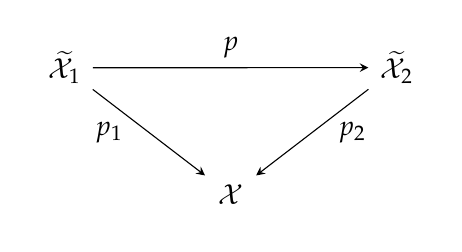
\begin{tikzpicture}
		\matrix (m) [matrix of math nodes,row sep=3em,column sep=4em,minimum width=2em]
		{
			\widetilde{\mathcal X}_1 & &\widetilde{\mathcal X}_2\\ 
			& {\mathcal X}\\};
		\path[-stealth]
		(m-1-1) edge node [above] {$p$} (m-1-3)
		(m-1-1) edge node [left]  {$p_1~~$} (m-2-2)
		(m-1-3) edge node [right] {$~~p_2$} (m-2-2);
	\end{tikzpicture}
	\\
	where $\sX$ is locally connected (cf. Definition \ref{top_locally_connected_defn}) and $p_1$, $p_2$ are covering projections. If $p$ is a surjection then $p$ is a covering projection.
	\end{corollary}
	\begin{theorem}\label{top_locally_conn_cov_com_thm}\cite{spanier:at}
	If   $p: \widetilde{\mathcal X}\to {\mathcal X}$ is a covering projection onto locally connected base space, then for any component  $\widetilde{\mathcal Y}$ of $\widetilde{\mathcal X}$ the map
	$$
	p|_{\widetilde{\mathcal Y}}:\widetilde{\mathcal Y} \to p\left(\widetilde{\mathcal Y} \right) 
	$$
	is a covering projection onto some component of $\widetilde{\mathcal X}$.
	\end{theorem}
	%\begin{lemma}\label{top_covp_cat_lem}  	\ref{top_finite_covering_thm}}
	%In the {category of connected covering spaces} of a connected locally path-connected space every morphism is itself a covering projection.
	%\end{lemma}
	\begin{theorem}\label{top_conjugate_thm}\cite{spanier:at}
	Let $p_1: 	\widetilde{\sX}_1 \to \sX$, $p_2: 	\widetilde{\sX}_2 \to \sX$ be objects  in the category of connected covering spaces of a connected locally path-connected space $\sX$. The following are equivalent
	\begin{enumerate}
		\item [(a)] There is a covering projection $f:\widetilde{\sX}_1 \to \widetilde{\sX}_2$ such that $p_2 \circ f = p_1$.
		\item[(b)] For all $\widetilde{x}_1\in \widetilde{\sX}_1$ and  $\widetilde{x}_2\in \widetilde{\sX}_2$ such that $p_1\left(\widetilde{x}_1 \right) = p_2\left(\widetilde{x}_2 \right)$, $\pi_1\left(p_1\right)\left( \pi_1 \left( \widetilde{\sX}_1, \widetilde{x}_1\right)  \right)$ is conjugate to a subgroup of  $\pi_1\left(p_2\right)\left( \pi_1 \left( \widetilde{\sX}_2, \widetilde{x}_2\right)  \right)$.
		\item[(c)] There exist $\widetilde{x}_1\in \widetilde{\sX}_1$ and  $\widetilde{x}_2\in \widetilde{\sX}_2$ such that $\pi_1\left(p_1\right)\left( \pi_1 \left( \widetilde{\sX}_1, \widetilde{x}_1\right)  \right)$ is conjugate to a subgroup of  $\pi_1\left(p_2\right)\left( \pi_1 \left( \widetilde{\sX}_2, \widetilde{x}_2\right)  \right)$.
	\end{enumerate} 
	\end{theorem}
	\begin{definition}\label{local_homeomorphism_defn}\cite{spanier:at}
	A continuous map $f: \sX \to \sY$ is called a \textit{local homeomorphism} if each 
	point $y \in \sY$ has an open neighbourhood mapped homeomorphically by $f$ onto 
	an open subset of $\sX$
	\end{definition}
	\begin{lemma}\label{top_cov_lem}\cite{spanier:at}
	A covering projection is a local homeomorphism.
	\end{lemma}
	
	\begin{lemma}\label{top_om_lem}\cite{spanier:at}
	A local homeomorphism is an open map (cf. Definition \ref{top_onen_map_defn}).
	\end{lemma}
	
	
	\begin{remark}\label{top_cov_bicont_rem}
	From the Lemmas \ref{top_om_lem} and \ref{top_om_lem} it follows that any covering is a bicontinuous map (cf. Definition \ref{top_bicont_defn}).
	\end{remark}
	
	
	
	\begin{defn}\label{top_path_lifting_defn}\cite{spanier:at}
	A continuous map $p:\mathcal{E} \to \mathcal{B}$ is said to have the {\it unique path lifting} if, given paths $\omega$ and $\omega'$ in $E$ such that $p \circ \omega = p \circ \omega'$ and $\omega(0)=\omega'(0)$, then $\omega=\omega'$.
	\end{defn}
	\begin{thm}\cite{spanier:at}\label{spanier_thm_un}
	Let $p: \widetilde{\mathcal{X}} \to \mathcal{X}$ be a covering projection and let $f, g: \mathcal{Y} \to \widetilde{\mathcal{X}}$ be liftings of the same map (that is, $p \circ f = p \circ g$). If $\mathcal{Y}$ is connected and $f$ agrees with g for some point of $\mathcal{Y}$ then $f=g$.
	\end{thm}
	\begin{rem}
	From theorem \ref{spanier_thm_un} it follows that a covering projection has unique path lifting.
	\end{rem}
	
	\subsubsection{Regular and universal coverings}
	\begin{defn}\label{top_regular_defn}\cite{spanier:at}
	A fibration $p: \mathcal{\widetilde{X}} \to \mathcal{X}$ with unique path lifting is said to be  {\it regular} if, given any closed path $\omega$ in $\mathcal{X}$, either every lifting of $\omega$ is closed or none is closed.
	\end{defn}
	\begin{thm}\label{locally_path_thm}\cite{spanier:at}
	Let $p: \widetilde{\mathcal X} \to \mathcal X$ be a fibration with unique path lifting and assume that a nonempty $\widetilde{\mathcal X}$ is a locally path-connected space. Then $p$ is regular if and only if for some $\widetilde{x}_0 \in  \widetilde{\mathcal X}$, $\pi_1\left(p\right)\pi_1\left(\widetilde{\mathcal X}, \widetilde{x}_0\right)$ is a normal subgroup of $\pi_1\left(\mathcal X, p\left(\widetilde{x}_0\right)\right)$.
	\end{thm}
	\begin{definition}\label{top_properly_disc_group_defn}\cite{spanier:at} 
	A group $G$ of homeomorphisms of a topological space $\sY$  is said to be  
	\textit{discontinuous} if the orbits of $G$ in $\sY$ are discrete subsets of $\sY$. $G$ is \textit{properly discontinuous} if for $y \in \sY$ there is an open neighbourhood $\sU$ of $y$ in $\sY$ such 
	that if $g, g' \in  G$ and $g\sU$ meets $g'\sU$, then $g = g'$. $G$ \textit{acts without fixed points} if the only element of $g\in G$ having fixed points is the identity element.	
	\end{definition}
	\begin{remark}\label{top_properly_disc_rem}\cite{spanier:at}
	A finite group of homeomorphisms acting without fixed points on a 
	Hausdorff space is properly discontinuous.
	\end{remark}
	\begin{theorem}\label{top_group_of_covering_transformations_thm}\cite{spanier:at}
	Let $G$ a properly discontinuous group of homeomorphisms 
	of a space $\sY$. Then the projection of $\sY$ to the orbit space $\sY/G$ is a covering projection. If $\sY$ is connected, this covering projection is regular and $G$  is its	group of covering transformations. 
	\end{theorem}
	\begin{lem}\label{top_cov_from_pi1_cor}\cite{spanier:at}
	Let $p: \widetilde{\mathcal X} \to \mathcal X$ be a fibration with a unique path lifting. If $ \widetilde{\mathcal X}$ is connected and locally path-connected and $\widetilde{x}_0 \in \widetilde{\mathcal X}$ then $p$ is regular if and only if $G\left(\widetilde{\mathcal X}~|~{\mathcal X} \right)$ principal  \ref{top_principal_defn} ly acts on each fiber of $p$, in which case 
	$$
	\psi: G\left(\widetilde{\mathcal X}~|~{\mathcal X} \right) \approx \pi_1\left(\mathcal X, p\left( \widetilde{x}_0\right)  \right) / \pi_1\left( p\right)\pi_1\left(\widetilde{\mathcal X}, \widetilde{x}_0 \right)  
	$$
	where $\pi_1$ denotes fundamental groups (cf. Remark \ref{top_homotopy_group_rem}).
	\end{lem}
	\begin{remark}\label{top_sim_con_reg_rem}\cite{spanier:at}
	If $\widetilde{   \sX}$ is simply connected, any fibration $p: \widetilde{   \sX} \to \sX$ is regular, and we also have the next result.
	\end{remark}
	\begin{cor}\label{top_cov_pi1_cor}\cite{spanier:at}
	Let $p: \widetilde{\mathcal X} \to \mathcal X$ be a fibration with a unique path lifting where $ \widetilde{\mathcal X}$ is simply connected locally path-connected and nonempty.  Then the group of self-equivalences of $p$ is isomorphic to the fundamental group of ${\mathcal X}$ (cf. Remark \ref{top_homotopy_group_rem}), i.e. $\pi_1\left( {\mathcal X}\right)\approx G\left(\left.\widetilde{\sX}~\right|\sX\right)$.  
	\end{cor}
	
	\begin{theorem}\label{top_gr_cov_thm}\cite{spanier:at}
	%13 theorem
	Let $\sX$ be a connected locally path-connected space and let 
	$x_0\in \sX$. Let $H$ be a subgroup of $\pi_1\left( \sX, x_0\right)$  and assume  there is an open  
	covering $\mathscr U$ of $\sX$ such that $\pi_1\left(\mathscr U, x_0 \right)\subset H$ . Then there is a covering projection $p:\left(  \widetilde \sX, \widetilde x_0\right) \to \left(\sX, x_0 \right)$ such that  $p_{\#}\left(\widetilde \sX, \widetilde x_0 \right)= H$ . 
	\end{theorem}
	
	\begin{definition}\label{top_universal_covering_defn}\cite{spanier:at}
	A \textit{universal covering space} of a connected space $\sX$ is an object $p: \widetilde{\sX}\to \sX$ of the category of connected covering spaces of $\sX$ such that for any object $p': \widetilde{\sX}'\to \sX$ of this category there is a morphism 
	\newline
	\begin{tikzpicture}
		\matrix (m) [matrix of math nodes,row sep=3em,column sep=4em,minimum width=2em]
		{
			\widetilde{\sX}  &  & \widetilde{\sX}'\\
			& \sX & \\};
		\path[-stealth]
		(m-1-1) edge node [above] {$f$} (m-1-3)
		(m-1-1) edge node [left]  {$p~~$} (m-2-2)
		(m-1-3) edge node [right] {$~~p'$} (m-2-2);
		%\draw[dashed,->]   (m-1-1) -- (m-1-3);
	\end{tikzpicture}
	\\
	in the category.
	\end{definition}
	
	\begin{lem}\label{top_simply_con_cov_lem}\cite{spanier:at}
	A connected locally path-connected space $\mathcal X$ has a simply connected covering space $\widetilde{\sX}$ if and only if  $\mathcal X$ is semilocally 1-connected (cf. Definition \ref{top_semi1_defn}).
	\end{lem}
	\begin{remark}\label{top_simply_con_cov_rem}
	Under the hypothesis of the Lemma \ref{top_simply_con_cov_lem} there is an isomorphism
	$$
	\pi_1\left(\sX, x_0 \right)\cong G\left(\left.\widetilde \sX \right| \sX\right).  
	$$
	\end{remark}	
	%\begin{lem}\label{top_simply_con_uni_cor}\cite{spanier:at}
	%	Any universal covering space of a connected locally path connected semilocally 1-connected space is simply connected.
	% \end{lem}
%\begin{lem}\label{top_uni_spa_lem}\cite{spanier:at}
% 	Two universal covering spaces of a connected locally path-connected space are equivalent.
% \end{lem}

\begin{lem}\label{top_uni_exist_spa_lem}\cite{spanier:at}
A simply connected covering space of a connected locally path-connected space $\sX$ is an universal covering space of $\sX$.
\end{lem}






\begin{prop}\cite{switzer:at} \label{top_pi1_pi1_prop}
(cf. Proposition 3.30).
If $\sX$ is a topological space then there is an action of $\pi_1\left(\sX\right)\times \pi_1\left(\sX\right)\to \pi_1\left(\sX\right)$ given conjugation; i.e. such that for $\ga, \a \in \pi_1\left(\sX\right)$ one has $\ga \cdot \a = \ga \a\ga^{-1}$.
\end{prop}
	\section{Measure theory}\label{mea_th_sec}


\paragraph{} The notion of the \textit{Radon measure} is described in \cite{bogachev_measure_v1}.
%	\begin{theorem}\label{radon_repr_thm}\cite{bogachev_measure_v2} (Riesz representation theorem)
	%$Theorem. 7.10.4 $
	%		Let $K$ be a compact space. Then, for every continuous linear functional $L$ on the Banach space $C\left(K \right)$ , there exists a unique
	%		\textit{Radon measure} $\mu$ such that
	%		$$
	%		L\left(f \right) = \int_{K} f ~\d\mu \quad \forall f \in C\left(K \right). 
	%		$$
	%	\end{theorem}


\begin{theorem}\label{meafunc_thm}\cite{bogachev_measure_v2}
	% 7.11.3. Theorem. 
	Let $\sX$ be a locally compact space and let $L$ be a linear
	function on $C_c\left(\sX \right)$  such that $L\left(f\right)\ge 0$ if $f\ge 0$. Then, there exists a Borel
	measure $\mu$ on $\sX$ with values in $\left[0, +\infty\right]$ such that
	\be\label{meafunc_eqn}
	L\left(f \right) = \int_{\sX} f~ d\mu \quad \forall f \in C_0\left(\sX \right).
	\ee
	In addition, one can choose $\mu$ in such a way that it will be Radon on all sets of finite measure %(and even inner compact regular on B(X),
	and there is only one measure with this property).
\end{theorem}
\begin{remark}
	In \cite{bogachev_measure_v2} the space of $C_c\left( \sX\right)$ is denoted by  $C_0\left( \sX\right)$.
\end{remark}

\begin{defn}\label{measure_image_defn} Definition \cite{bogachev_measure_v2}
	Let $\mu$ be a Borel measure on a topological space $\mathcal{X}$ and let $f$ be a $\mu$- measurable mapping from $\mathcal{X}$ to a topological space $\mathcal{Y}$. Then on $\mathcal{Y}$ we obtain
	the Borel measure $\nu = \mu \circ f^{-1}: B \mapsto \mu \circ f^{-1}\left( B\right)$. The measure $\nu$ is called
	the \textit{image} of $\mu$ under the mapping $f$, and $\mu$ is called a \textit{preimage} of $\nu$. The  same terms are used in the case of general measurable mappings of measurable  spaces.
\end{defn}




\begin{thm}\label{comm_image_thm}\cite{bogachev_measure_v2}
	Let $ \mathcal{X}$ and $\mathcal{Y}$ be two Hausdorff spaces. 	Let $f : \mathcal{X}\to \mathcal{Y}$ be a continuous mapping. If a measure $\mu$ on $\mathcal{X}$ is Radon, then so is $\mu \circ f^{-1}$.
\end{thm} 
 \begin{thm}\label{comm_mea_preimage_thm}\cite{bogachev_measure_v2}
	 	Let $f$ be a mapping from a topological space $\mathcal X$ to a 	topological space $\mathcal Y$ with a Radon measure $\nu$. Suppose that there exists an increasing sequence of compact sets $K_n \subset \mathcal X$ such that $f$ is continuous on every $K_n$ and 
		\begin{equation*}
		 		\lim_{n \to \infty } \left|\nu\right|f\left(K_n \right) = \left\|\nu\right\|.
			\end{equation*}
		Then, there exists a Radon measure $\mu$ on $\mathcal X$ with $\mu \circ f^{-1} = \nu$. In addition, 	this measure can be chosen with the property $\left\|\nu\right\| = \left\|\mu\right\|$. In particular, this 	is true if $\mathcal X$ and $\mathcal X$ are compact and $f$ is a continuous surjection.
	\end{thm}
	%Proposition 7.2.3.
	 \begin{prop}\cite{cohn_measure}
		 	Let $\mathcal X$ be a locally compact Hausdorff space that has a countable  base, and let $\mu$ be a Borel measure on $\mathcal X$ that is finite on compact sets. Then $\mu$ is regular.
		\end{prop} 
		
			\begin{empt}
					We need the notion of essential support  functions described in \cite{elliot:an}. For a given Borel measure $\mu$ let $f$ be a Borel-measurable function. Consider the collection $\widetilde{\Om}$ of open subsets $\om$ with the property that $f\left(x \right)=0$ for $\mu$-almost every $x \in \om$ and let the open set $\om^*$ be the union of all $\om$'s in  $\widetilde{\Om}$.
				\end{empt}
			\begin{defn}\label{essential_support_defn}
			 	The  \textit{essential support} of $f$ or $\mathfrak{ess~supp}\left( f\right)$ is the complement of $\om^*$. There is the following formula
			 	$$
			 	\mathfrak{ess~supp}\left( f\right) = \mathcal X \setminus \bigcup \left\{\om \in \mathcal X~|~ \om \text{ is open and } f=0~\mu-\text{almost everywhere in }\om\right\}.
			 	$$
				If $x \notin \mathfrak{ess~supp}\left( f\right)$ then there is an open neighbourhood $\mathcal U$ of $x$ and representative $\varphi$ of $f$ such that $\varphi\left({\mathcal U}\right) = \{0\}$. 
				\end{defn}


\section{Regularization}
 In physics, especially quantum field theory, regularization is a method of modifying observables which have singularities in order to make them finite by the introduction of a suitable parameter called the regulator. The regulator, also known as a "cutoff", models our lack of knowledge about physics at unobserved scales (e.g. scales of small size or large energy levels). It compensates for (and requires) the possibility of separation of scales that "new physics" may be discovered at those scales which the present theory is unable to model, while enabling the current theory to give accurate predictions as an "effective theory" within its intended scale of use.
 
 It is distinct from renormalization, another technique to control infinities without assuming new physics, by adjusting for self-interaction feedback.
 
 Regularization was for many decades controversial even amongst its inventors, as it combines physical and epistemological claims into the same equations. However, it is now well understood and has proven to yield useful, accurate predictions
 \section{Geometric quantization}
 \paragraph{} Here I follow to \cite{hawkins:nc_reg}.
\label{GQ}
We can maintain much greater symmetry with noncommutative approximating 
algebras.  Geometric quantization provides a method of constructing 
noncommutative approximations.  

As the name suggests, geometric quantization was originally intended 
as a systematic mathematical procedure for constructing quantum 
mechanics from classical mechanics.  Geometric quantization applies to 
a symplectic manifold (originally, phase space) with some additional 
structure (a ``polarization'').  The terminology of quantization is 
unfortunate here, since I am concerned with quantum field theory.  
Insofar as geometric quantization goes here, the manifold is not to be 
interpreted as phase space, the Hilbert spaces are not to be 
interpreted as spaces of quantum-mechanical states, and the algebras 
do not consist of observables.  In this paper, ``quantization'' and 
``quantum'' have nothing to do with each other.

Here I shall use geometric quantization with a ``complex 
polarization''\!.  For a compact K\"{a}hler manifold, $\M$, this 
generates a sequence of finite-di\-men\-sion\-al matrix algebras 
$\AN$ which approximate the algebra $\C^\infty(\M)$ in a sense 
that I shall explain below.

A K\"{a}hler manifold is simultaneously a Riemannian, symplectic, and 
complex manifold.  These structures are compatible with each other, 
such that raising one index of the symplectic 2-form, $\omega$, with 
the Riemannian metric gives the complex structure\footnote{A 2-index 
	tensor such that $J^i_{\;j}J^j_{\;k}=-\delta^i_k$.} $J$.  I shall 
assume, for a length $R$ (roughly, the size of $\M$), that the 
integral of $\frac\omega{2\pi R^2}$ over any closed 2-surface is an 
integer; this implies the existence of a line bundle 
(1-di\-men\-sion\-al, complex vector bundle), $L$, with a connection 
$\nabla$ and curvature $R^{-2}\omega$.  If $\M$ is simply connected, 
then $L$ is unique.

There is also a unique fiberwise, Hermitian inner product on $L$ 
compatible with the connection.  Given two sections 
$\psi,\varphi\in\G(\M,L)$, their inner product is a function 
$\bar\psi\varphi\in\C(\M)$. Compatibility with the connection means 
that for smooth sections, 
$d(\bar\psi\varphi)=\nabla\bar\psi\, \varphi+\bar\psi\nabla\varphi$. 
Using the fiberwise inner product, we can construct a global inner 
product,
\bean
\langle\psi\mid\varphi\rangle \bydef \int_M \bar\psi\varphi\, \epsilon
\mbox.\label{inner.product}\eean
It is an elementary property of any K\"{a}hler manifold that the 
Riemannian volume form can also be written in terms of the symplectic 
form as $\epsilon = \frac{\omega^n}{n!}$, where $2n=\dim\M$.

A holomorphic section of $L$ is one satisfying the differential 
equation $J\nabla\psi=i\nabla\psi$, or in index notation 
$J_{\;i}^{j}\psi_{|j} = i\psi_{|i}$.  The space of holomorphic 
sections $\Gh(\M,L)$ is finite dimensional, and the inner product, 
\eqref{inner.product}, makes it a Hilbert space.  

With this notation and structure, I can now present the geometric 
quantization construction.  The tensor power bundle $L^{\otimes N}$ 
is much like $L$; it is a line bundle with an inner product,
but with curvature $NR^{-2}\omega$.  As $N$ increases, the spaces of  
holomorphic sections are increasingly large, 
finite-dimensional Hilbert spaces, 
\[
\HN:=\Gh(\M,L^{\otimes N})
\mbox.\]
The 
dimension of $\HN$ grows as a polynomial in $N$ (given by the 
Riemann-Roch formula, Eq.~\eqref{riemann-roch}).  The algebra $\AN$ is 
now defined as 
\[
\AN:=\End\HN \mbox;\] 
that is, the space of $\C$-linear maps from $\HN$ to itself --- in 
other words, matrices over $\HN$.  The inner product on $\HN$ gives 
$\AN$ an involution (Hermitian adjoint) $a\mapsto a^*$; this makes 
$\AN$ a finite-dimensional $C^*$-algebra.

The collection of algebras $\{\AN\}$ alone knows nothing of $\M$.  In 
order to connect $\AN$ with $\M$, we will need a structure such as the 
Toeplitz quantization map $T_N:\C(\M)\onto\AN$.  For any function 
$f\in\C(\M)$, the matrix $T_N(f)$ is defined by giving its 
action on any $\psi\in\HN$.  Since $\psi$ is a section of $L^{\otimes 
	N}$, the product $f\psi$ is also a (not necessarily holomorphic) 
section of $L^{\otimes N}$.  Using the inner product 
\eqref{inner.product} we can project $f\psi$ orthogonally back to 
$\HN$ and call this $T_N(f)\psi$.  This implicitly defines $T_N$.

If $\M$ were a phase space then 
$T_N(f)$ would be interpreted as the quantum observable, $\hat f$, 
corresponding to $f$.  The Toeplitz maps have the important property 
of being \emph{approximately} multiplicative; that is, for any two 
continuous functions on $\M$,
\[
\lim_{N\to\infty} \norm{T_N(f)T_N(g)-T_N(fg)} =0
\mbox.\]

According to Rieffel \cite{rie1}, quantization should be expressed in 
terms of a continuous field of $C^*$-algebras.  A continuous field $\Af$ 
of $C^*$-algebras over a compact topological space $\B$ is essentially a 
vector bundle whose fibers are $C^*$-algebras (see \cite{dix,k-w1}).  
The space of continuous sections $\G(\B,\Af)$ is a $C^*$-algebra.  For 
every point $b\in\B$, the evaluation map from $\G(\B,\Af)$ onto the 
fiber over $b$ is a $*$-homomorphism (a $C^*$-algebra map).  The product 
of a continuous function on $\B$ with a continuous section of $\Af$ is 
again a continuous section of $\Af$.  A continuous field of 
$C^*$-algebras is completely specified by describing its base space, its 
fibers, and which sections are continuous.

The geometric quantization of $\M$ leads to a natural continuous field 
of $C^*$-al\-ge\-bras, $\Af$.  The fibers of $\Af$ are each of the 
algebras $\AN$ and  $\C(\M)$.  This is one algebra for 
every natural number $N\in\N=\{1,2,\dots\}$, plus one extra.  The 
notion is that the sequence of algebras $\A_1,\A_2,\A_3,\ldots$ tends 
toward $\C(\M)$, so the natural topology for the base space is the 
one-point compactification $\Nhat=\N\cup\{\infty\}$, in which $\infty$ 
is the limit of any increasing sequence.  The field $\Af$ is 
implicitly defined by the requirement that for every $f\in\C(\M)$, 
there exists a section $T(f)\in\G(\Nhat,\Af)$ whose evaluation at $N$ 
is $T_N(f)$ and at $\infty$ is $f$.

The existence of this continuous field is the sense in which the 
algebra $\AN$ approximates $\C(\M)$, but we can do better than this.  
There is a sense in which $\AN$ approximates the algebra of smooth 
functions $\Coo(\M)$.  As I discussed in \cite{haw5}, the field $\Af$ 
has a further structure as a sort of \emph{smooth} field of 
$C^*$-algebras.

Obviously, our base space, $\Nhat$ is not a manifold.  However, there 
is a reasonable notion of smooth functions on $\Nhat$.  We can 
identify $\Nhat$ with the homeomorphic set 
$\{1,\frac12,\frac13,\dots,0\}\subset\R$, and define the smooth 
functions $\Coo(\Nhat)$ as those which are restrictions of smooth 
functions on $\R$.  Equivalently, a smooth function on $\Nhat$ is one 
which can be approximated to arbitrary order by a power series in 
$N^{-1}$.

The smooth structure of $\Af$ is given by a dense $*$-subalgebra 
$\Ga^\infty(\Nhat,\Af)\subset\G(\Nhat,\Af)$ of ``smooth'' sections.  The 
product of a smooth function on $\Nhat$ with a smooth section of $\Af$ 
is again a smooth section of $\Af$.  The evaluation of any smooth 
section at $\infty$ is a smooth function on $\M$.  The algebra 
$\Ga^\infty(\Nhat,\Af)$ is essentially defined by the condition that any 
smooth function $f\in\Coo(\M)$ gives a smooth section 
$T(f)\in\Ga^\infty(\Nhat,\Af)$.
\section{The Regularized Action}
\label{regularized.action}
For a single real scalar field, $\phi\in\Coo(\M)$, the general, 
unregularized action functional is
\bean
S[\phi] := \int_M \left[\tfrac12(\nabla\phi)^2 + \tfrac12m^2\phi^2 
+ V(\phi)\right]\epsilon 
\mbox,\label{general.action}\eean
where $\epsilon$ is the volume form on $\M$, and $V$ is a 
lower-bounded polynomial self-coupling.  Complex conjugation on 
$\Coo(\M)$ corresponds to the adjoint on $\AN$, so our approximation to 
the space of real functions on $\M$ will be the subspace 
$\AN^\mathrm{s.a.}\subset\AN$ of self-adjoint elements.  To construct 
the regularized theory, we need a regularized action defined on 
$\AN^\mathrm{s.a.}$ that approximates \eqref{general.action}.

Let's be precise about what it means to approximate an action 
functional in this way.  We need a sequence of action functionals, 
$S_N:\AN^\mathrm{s.a.}\to\R$, which converge to the unregularized 
action $S$.  This is nontrivial to define because these are functionals 
on different spaces.  Let $\phi\in\Ga^\infty(\Nhat,\Af)$ 
be an arbitrary, self-adjoint, smooth section, and denote its 
evaluations as $\phi_N\in\AN$; the sequence $\{\phi_N\}$ can be 
considered to converge 
well to the smooth function $\phi_\infty\in\Coo(\M,\R)$.  My 
definition for convergence of $\{S_n\}$ is simply that for any such 
$\phi$,
\[
\lim_{N\to\infty} S_N(\phi_N) = S[\phi_\infty]
\mbox.\]

Several ingredients are needed to construct a regularized action.  The 
simplest is the product.  It is the most elementary property of 
geometric quantization that multiplication in $\Coo(\M)$ is 
approximated by multiplication in $\AN$.

The normalized trace on $\AN$ approximates the normalized 
integral on $\M$. That is, for any $a\in\Ga^\infty(\Nhat,\Af)$,
\[
\ntr a_N \equiv \frac{\tr a_N}{\tr 1} = \frac1{\vol\M}\int_M a_\infty 
\epsilon + \Or^{-1}(N)
\mbox.\]

The unregularized kinetic term can be written in terms of the Laplacian, 
$\Delta=-\nabla^2$,  using the 
elementary identity,
\[
\int_M (\nabla\phi)^2\epsilon = \int_M \phi \,\Delta(\phi) \epsilon
\mbox.\]
Mimicking this, we can safely write the regularized kinetic term as
\[
\vol(\M)\, \ntr \left[\tfrac12 \phi 
\,\Delta(\phi)\right]
\mbox,\]
since in fact, \emph{any} quadratic functional can be written in this form. 

In the coadjoint orbit case, which I will mainly discuss, the 
Laplacian is simply a multiple of the quadratic Casimir operator.  
However, the discussion in this section will apply equally to any 
K\"{a}hler manifold for which a suitable approximate Laplacian can be 
constructed.  For this reason, I will write the approximate Laplacian 
as $\Delta$ until a more explicit form is required for examples.

The regularized action approximating \eqref{general.action} is (using 
$\tr 1 =\dim\HN$)
\bean
S_N(\phi) = \frac{\vol\M}{\dim\HN} \tr \left[\tfrac12 \phi \,\Delta(\phi) + 
\tfrac12m^2\phi^2 + V(\phi)\right]
\mbox.\label{regact}\eean
This regularized action was originally formulated by Grosse, 
Klim\v{c}\'{\i}k, and Pre\v{s}\-naj\-der \cite{g-k-p1} in the special case 
of $S^2$; however, the corresponding perturbation theory has not 
previously been discussed in detail.

\subsection{The commutative limit}
Using the action, \eqref{regact} we can now define the regularized 
theory using a path integral formula,
\bean
Z\cdot\langle0\rvert F(\hat\phi) \lvert0\rangle := 
\int_{\AN^\mathrm{s.a.}} F(\phi) 
e^{-S_N(\phi)} d\phi
\mbox.\label{pathint2}\eean
This is formally identical to Eq.~\eqref{pathint}, but it differs in 
that it is not merely a formal expression.  The measure $d\phi$ is 
simply the Lebesgue measure on the finite-dimensional vector space 
$\AN^\mathrm{s.a.}$.  Because $S_N(\phi)$ increases at least 
quadratically in all directions, Eq.~\eqref{pathint2} is finite for 
all polynomial functionals $F$.

In the standard lattice regularization, it is necessary to verify that 
a theory is sufficiently well behaved in the ``continuum limit'' as 
the regularization is removed.  The limit of removing the 
regularization in the present case is the commutative limit, 
$N\to\infty$.  At this stage, it is not entirely clear what the 
correct definition of convergence in the commutative limit should be.

Certainly, renormalization is necessary. That is, the bare mass, $m$, 
and coupling constants (the coefficients in $V$) must depend on $N$, 
and the field $\phi$ must also be renormalized by an $N$-dependent factor. 
Some condition of convergence is then applied to the sequence of 
renormalized, regularized theories.

A plausible form of the convergence condition is in terms of the 
one-particle irreducible generating functionals, $\G_N$.  These are 
functions $\G_N:\AN^\mathrm{s.a.}\to\R$, derived from the 
path-integral.  If the generating functionals are renormalized so that 
$\G_N(0)=0$, then the condition may be that for any smooth, 
self-adjoint section $\phi\in\Ga^\infty(\Nhat,\Af)$, with evaluations 
$\phi_N\in\AN$, the sequence $\{\G_N(\phi_N)\}$ is convergent.

The derivation of Feynman rules from the path integral can now proceed 
in essentially the standard, heuristic way (see, e.~g., \cite{pok}), 
except that now it is not just a formal calculation.  

\subsection{Green's functions}
Before we can discuss perturbation theory on a noncommutative space, 
we must first understand what Green's functions are from an 
algebraic perspective. I begin in greater generality than just a 
scalar field. 

In general, the space of classical field configurations, $\Phi$, need 
not be a vector space.  Such is the case for nonlinear 
$\sigma$-models.  However, for a free field theory, $\Phi$ is always a 
vector space.  Since we are going to apply perturbation theory about a 
free field theory, we must assume that $\Phi$ is a vector space here.

A Green's function is the vacuum expectation value of a product of 
fields.  An expectation value of a quantum field $\hat\phi$ is an 
element of the space of classical field configurations, $\Phi$, since 
$\hat\phi$ is thought of as a quantum field valued in $\Phi$.  An 
expectation value of a product of two fields is an element of the 
(real) tensor product $\Phi\otimes\Phi$.  Carrying on like this, we 
see that a $k$-point Green's function is an element of the real tensor 
power $\Phi^{\otimes k}$.  The use of real tensor products here is 
actually not restrictive; for a complex field, $\phi$, a real tensor 
product will include all possible combinations of $\phi$ and its 
conjugate field.

Actually, I am overoptimistically allowing a great deal to fall 
into the ambiguity in a tensor product of infinite dimensional spaces.
In the case of a real scalar field, $\Phi=\Coo(\M,\R)$, so the tensor 
product $\Phi\otimes\Phi$ should intuitively be a space of functions 
of two points on $\M$. Indeed, a 2-point Green's function for a 
scalar field is a function of two points; however, it has a 
singularity where the points coincide. This shows that the tensor 
product needs to be interpreted liberally. Fortunately this issue is 
irrelevant to the case at hand. Once $\Phi$ is finite-dimensional, 
there is no ambiguity in the tensor product.

In discussing divergences, one deals primarily with 
one-particle-irreducible % !!!\linebreak (\opi) Green's functions.  These 
can be constructed as derivatives of an $\R$-valued generating 
functional on $\Phi$.  This shows immediately that a $k$-point, !!! % \opi\ 
Greens function is a linear map from $\Phi^{\otimes k}$ to $\R$.  
One-particle-irreducible Green's functions thus live in the dual space 
of the corresponding ordinary Green's functions.

Because of the coefficient in front of the action, there are powers of 
(in the case of \eqref{regact}) $C=\tfrac{\vol\M}{\dim\HN}$ coming 
from the vertices and propagators.  If, instead of setting $\hbar=1$, 
we had kept explicit factors of $\hbar$, then the combination $\hbar 
C$ multiplying the action would be the only appearance of $\hbar$ in 
the functional integral.  This means that the overall power of $C$ for 
a Feynman diagram is the same as the overall power of $\hbar$ --- 
namely, the number of loops plus $1$.

Actually, implicit in most action functionals is an inner product on 
$\Phi$.  This means that $\Phi$ can be more or less naturally 
identified with a subspace of $\Phi^*$ in general, and with all of 
$\Phi^*$ when it is finite-dimensional.

This inner product on $\Phi$ tends to suffer an ambiguity of 
normalization.  The most natural inner product of two functions is given 
by multiplying them and integrating.  The most natural inner product 
on $\AN$ is given by multiplying matrices and taking the trace.  
Unfortunately, these inner products disagree when we pair $1$ with 
itself.  In $\C(\M)$ that gives $\vol\M$; in $\AN$ it gives $\dim\HN$.  
We must correct the inner product on $\AN$ by a factor of $C$, for 
consistency with that on functions.

The natural form of the !!! % \opi\ Green's functions is not actually the 
most useful normalization for comparison with the results of standard 
perturbation theory.  In practice, we deal with ordinary Feynman 
diagrams in momentum space.  The quantities we usually deal with are 
not the momentum-space Green's functions themselves, but have an overall, 
momentum-conserving $\delta$-function divided out.  

Consider 2-point Green's functions in a scalar theory. In momentum 
space, with the $\delta$-function divided out, these are simply 
functions of a single momentum. Multiplying two such functions in 
momentum space corresponds to convolution of Green's functions. In 
this normalization, a 2-point Green's function is a convolution 
operator; that is a linear map $\Phi\to\Phi$. 

In general, a $k$-point !!! % \opi\ Green's function in this normalization 
is a linear map $\Phi^{\otimes(k-1)}\to\Phi$.  In the regularized 
theory, this change simply amounts to dividing our amplitudes by $C$.  
This simplifies the Feynman rules slightly, so that the overall power 
of $C$ is now simply the number of loops.

\subsection{Noncommutative Feynman rules}
\label{feynman}
I'll now specialize to the theory given by the action \eqref{regact}, 
although most of the considerations are more general.  
As usual, the action splits into a free part (the first two terms) and 
an interaction part (the $V$ term).  The free part gives the 
propagator $(\Delta+m^2)^{-1}$; each monomial of $V(\phi)$ gives a 
vertex whose valence is the degree of the monomial.

A vertex of valence $r$ essentially represents the trace of a product 
of $r$ matrices.  The term corresponding to a standard Feynman diagram 
is a sum of terms with different orderings of the products.  It is 
convenient to represent these subterms diagrammatically.  For each 
vertex, the multiplicands correspond to incoming edges.  Because only 
the cyclic order matters in a trace, we only need to indicate a cyclic 
order to the edges.  This is easily done graphically by drawing the 
vertex in the plane.  The order of multiplication is indicated by the 
counterclockwise order of the attached edges.  The distinct terms are 
thus labeled by ``framings'' of the Feynman diagram in the plane.  

In ordinary quantum field theory involving a real field, there are 
symmetry factors to deal with. The contribution of a given diagram is 
divided by the number of its symmetries. In this case there is an 
additional type of combinatorial factor present. Since a given 
ordinary Feynman diagram corresponds to several framed diagrams, 
these framed diagrams are weighted by coefficients adding up to $1$. 
Determining these coefficients is a matter of enumerating the cyclic 
orientations of all vertices, and sorting the resultant framings into 
equivalence classes.

To express the exact Feynman rules, it is convenient to adapt the 
notation invented by 't~Hooft for discussing the large $N$ limit of 
$U(N)$-gauge theories (see \cite{tho,col}).  In that diagrammar, the 
gluon propagator is represented by a double line (two directed lines 
in opposite directions).  An outgoing arrow indicates an upper index 
and an ingoing arrow indicates a lower index.  The way lines are 
connected indicates how indices are contracted.  In these diagrams, the 
two lines of a gluon propagator do not touch.  This is appropriate, 
since they really have nothing to do with each other.  The propagator 
is not just invariant under $U(N)$, but under 2 separate actions of 
$U(N)$ corresponding to the 2 separate edges.

In the present context, however, the notation needs to be modified.  
The propagator is not invariant under arbitrary unitary 
transformations; it is only invariant under the isometries of $\M$ (if 
there are any).  The two lines of the propagator are thus no longer 
independent, and I indicate this by linked double lines as shown in 
Fig~\ref{propagator}.

The upper indices (outgoing arrows) are factors of $\HN$, while the 
lower indices (ingoing arrows) are factors of $\HN^*$.  Each factor of 
$\AN^\mathrm{s.a.}\subset \AN\subset \HN\otimes\HN^*$ thus gives an 
upper and a lower index, or an incoming and an outgoing arrow.

Figure~\ref{doubled} shows a more complicated doubled diagram.  Note 
that no distinction is made between overcrossings and undercrossings.


A reader might reasonably question that this is truly a regularization 
of \emph{real} scalar field theory.  After all, the subspace 
$\AN^\mathrm{s.a.}\subset\AN$ is not closed under multiplication, so 
why should these Feynman rules respect this subspace?  The issue is 
whether the Green's functions are self-adjoint, in the obvious sense 
for elements of a tensor power of $\AN$.  In fact, a given (framed) 
Feynman diagram may not be self-adjoint.  However, its adjoint is the 
mirror-image diagram, which is another framing of the same diagram and 
therefore contributes to the same Green's function.  This makes the 
Green's functions themselves self-adjoint, order-by-order in 
perturbation theory.

\
\section{Unrealistic Phenomena}
	
	\paragraph{}
	It is conjectured  that the $M$-theory can be represented as limit matrix model (cf. \cite{matrix_tori, bfss, ikkt} with finite-dimensional matrix. It is possible to obtain the  noncommutative toroidal compactification (cf. Appendix \ref{mat_tor_sec}) by infinite dimension matrix. However this solution is not realistic since infinite dimensional matrix yield infinite values of the given by the equation \eqref{ikkt_act_eqn} action functional. 
	The infinite dimensional matrix model is not realistic since 
	But physics can effectively operate with  unrealistic phenomena, i. e. phenomena which shall never occur. For example explained in \cite{isumaru} plain electromagnetic wave is not realistic. However this  "phenomenon" is effectively used in a lot of science and engineering calculations. If $\mathfrak{A}$ is a  $C^*$-realization (cf. Definition \ref{c_realization_defn}) of $d$-dimensional quantum physics then there is the natural inclusion $C_0\left(\R^d \right) \subset \mathfrak{A}$. According to the Appendix \ref{loc_mea_sec} one has  $\mathscr A \subset\mathfrak{A}_{\text{sa}}$  where $\mathscr A$ is the set of observables where $\mathfrak{A}_{\text{sa}}\subset \mathfrak{A}$ is the $\R$-subspace of self-adjoint operations. If $a \in C_0\left(\R^d \right)_{\text{sa}}\setminus C_c\left(\R^d \right)_{\text{sa}}$  then the volume of $\supp a$ is not finite. So a corresponding to the "observable" detector should have an infinite volume, i.e. $a$ corresponds to an unrealistic state. Note that $C_c\left(\R^d \right)$ is the Pedersen's ideal of $C_c\left(\R^d \right)$. According to my experience  the realistic phenomena are inside the Pedersen's ideal. 
	
	In \cite{landi:nm_nt,new_matrix} the necessary solution is associated with the inductive  limit of AT algebras, i.e. finite sums of $C\left(S^1 \right)\otimes \mathbb{M}_N\left( \C\right)$, Here we postulate that necessary solution equals to this limit.
	
		
	
	\section{Operator spaces and algebras}\label{oa_sec}
	\begin{definition}\label{op_space_defn}\cite{blecher_merdy}

		

		A concrete \textit{operator space} is a (usually closed) linear subspace $X$ of $B(\H_1,\H_2)$,
		for Hilbert spaces $\H_1,\H_2$ (indeed the case $\H_1=\H_2$ usually suffices, via the canonical
		inclusion $B(\H_1,\H_2)\subset B(\H_1\oplus\H_2)$.
	\end{definition}
	\begin{definition}\label{c_op_alg_defn}\cite{blecher_merdy}
		A \textit{concrete operator algebra} is a closed subalgebra of $B(\H)$, for some Hilbert space $\H$.
	\end{definition}
	\begin{remark}\label{c_op_alg_n_rem}
		Sometimes we consider operator algebras which are dense subalgebras of operator algebras.
	\end{remark}
	\begin{remark}\label{c_op_alg_rem}
		There are  abstract definitions of  \textit{operator algebras} and and an \textit{operator spaces}. It is proven that the classes of operator algebras and operator spaces are equivalent to the class of concrete operator algebras and spaces respectively (cf. \cite{blecher_merdy}.)
	\end{remark}
	\begin{definition}\label{op_u_space_defn}\cite{blecher_merdy}
		%1.3.1 
		(Unital operator spaces). We say that an operator space $X$ is \textit{unital} if it has a distinguished element usually written as $e$ or 1, called the \textit{identity} of $X$, 
		such that there exists a complete isometry $u: X \hookto A$ into a unital $C^*$-algebra with $u(e) = 1_A$. A \textit{unital-subspace} of such $X$ is a subspace containing $e$. 
	\end{definition}
	
	\begin{empt}\label{complete_maps_empt}\cite{blecher_merdy}
		%1.2.1 
		(Completely bounded maps). Suppose that $X$ and $Y$ are operator spaces 
		and that $u: X \to Y$ is a linear map. For a positive integer $n$, we write $u_n$ for 
		the associated map $[x_{jk} ] \mapsto \left[u\left(x_{jk}\right)\right]$ from $\mathbb{M}_n(X)$ to $\mathbb{M}_n(Y )$. This is often called the ($n^{\text{th}}$) amplification of $u$, and may also be thought of as the map $\Id_{\mathbb{M}_n\left( \C\right)} \otimes u$ on 
		$\mathbb{M}_n\left( \C\right)\otimes X$. Similarly one may define $u_{m,n} : \mathbb{M}_{m,n}(X) \to \mathbb{M}_{m,n}(Y)$. If each matrix 
		space $\mathbb{M}_n(X)$ and $\mathbb{M}_n(Y)$ has a given norm $\left\|\cdot \right\|_n$ , and if un is an isometry for 
		all $n\in \N$, then we say that $u$ is 
		\textit{completely isometric}, or is a \textit{complete isometry}. 
		Similarly, $u$ is \textit{completely contractive} (resp. is a \textit{complete quotient map}) if each 
		$u_n$ is a contraction (resp. takes the open ball of $\mathbb{M}_n(X)$ onto the open ball of $\mathbb{M}_n(Y )$). A map $u$ is completely bounded if 
		$$
		\left\| u\right\|_{\mathrm{cb}}  \stackrel{\mathrm{def}}{=}\sup\left\{\left.\left\| \left[u\left(x_{jk}\right)\right]\right\|~\right|~\left\| \left[ x_{jk}\right] \right\|< 1 \quad\forall n \in \N\right\} 
		$$
		Compositions of completely bounded maps are completely bounded, and one 
		has the expected relation $\left\| u\circ v\right\|_{\mathrm{cb}}\le \left\| u\right\|_{\mathrm{cb}}\left\| v\right\|_{\mathrm{cb}}$. If $u: X \to Y$ is a completely 
		bounded linear bijection, and if its inverse is completely bounded too, then we 
		say that $u$ is a complete isomorphism. In this case, we say that $X$ and $Y$ are 
		completely isomorphic and we write $X \approx Y$. 
		The matrix norms satisfy to the following \textit{Ruan's axioms}
	\end{empt}
	\begin{definition}
		The following conditions:
		\begin{itemize}
			\item[(R1)]  $\left\|\a x\bt \right\|_n \le \left\|\a \right\|\left\|x \right\|_n\left\|\bt \right\|$, for all  $n\in \N$ and all  $\a, \bt \in \mathbb{M}_n\left(\C\right)$ and $x \in \mathbb{M}_n\left(X\right)$
			(where multiplication of an element of $\mathbb{M}_n\left(X\right)$ by an element of $\mathbb{M}_n\left(\C\right)$ is
			defined in the obvious way).
			\item[(R2)]  For all $x\in\mathbb{M}_n\left(X\right)$ and $y\in\mathbb{M}_n\left(Y\right)$, we have
			$$
			\left\|\begin{pmatrix} x & 0\\
				0& y
			\end{pmatrix}\right\|_{n + m} = \max\left(\left\|x \right\|_n, \left\|y \right\|_m\right).
			$$
			
		\end{itemize}
		are said to be \textit{Ruan's axioms}.
	\end{definition}
			\begin{definition}
		%DEFINITION 0.1 (cf. 2.2.3 2 ). 
		A {\it quantum norm} on $E$ is a norm on $\F \times E$ (where $\F\subset B\left(\ell^2\left( \N\right)  \right) $ is the ideal of finite-rank operators), satisfying 
		the following two conditions ("Ruan's axioms"): 
		\begin{enumerate}
			\item [(RI)]  For every $a \in  B\left(\ell^2\left( \N\right)  \right)$ and ,  $u \in\F \otimes E$ we have 
			\bean
			\left\| ua\right\|,\quad  \left\| au\right\|   \le \left\| a\right\| \left\| u\right\| 
			\eean 
			\item [(RII)]  If, for $u, v \in \F \otimes E$, there exist projections (i.e., self-adjoint idempotents)  $P, Q\in  B\left(\ell^2\left( \N\right)  \right)$ such that $P \dot u \dot P = u$, $Q \dot  v \dot Q = v$ and $PQ=0$, then we have 
			\bean
			\left\| u+ v\right\| = \max  \left(\left\| u\right\|, \left\|  v\right\| \right) 
			\eean 
			An abstract operator space is a linear space, equipped with a quantum norm 
			(or, if we want to play a precisian, it is a pair (E, II. II), consisting of a linear space 
			and a quantum norm on it). Rather often, when it seems to be convenient, we use 
			the term quantum space instead of "abstract operator space". We emphasize that 
			both terms have absolutely the same meaning.
		\end{enumerate}
		
	\end{definition}
	
	\begin{remark}\label{c_star_iso_rem}\cite{blecher_merdy}
		Any $*$-homomorphism $u: A \to B$ of $C^*$-algebras is injective if and only if $u$ is completely isometric (cf. \cite{blecher_merdy}).
	\end{remark}
	\begin{empt}\label{blecher_merdy_empt}\cite{blecher_merdy}
		%4.2.3 
		(Extensions of operator spaces). An \textit{extension} of an operator space $X$ is 
		an operator space $Y$ , together with a linear completely isometric map $j : X\hookto Y$. 
		Often we suppress mention of $j$, and identify $X$ with a subspace of $Y$. We say that $Y$ is a \textit{rigid} extension of $X$ if $\Id_Y$ is the only linear completely contractive 
		map $Y\to Y$ which restricts to the identity map on $j\left( X\right)$. We say $Y$ is an \textit{essential} extension of $X$ if whenever $u: Y\to Z$ is a completely contractive map 
		into another operator space $Z$ such that $u\circ j$ is a complete isometry, then $u$ is a complete isometry. We say that $(Y, j)$ is an \textit{injective envelope} of $X$ if $Y$ is 
		injective, and if there is no injective subspace of $Y$ containing $j(X)$. 
	\end{empt}
	\begin{lem}\label{os_eqv_lem}
		Let $(Y, j)$ be an extension of an operator space $X$ such that $Y$ is 
		injective. The following are equivalent: 
		\begin{enumerate}
			\item[(i)] $Y$ is an injective envelope of $X$, 
			\item[(ii)] $Y$ is a rigid extension of $X$, 
			\item[(iii)] $Y$ is an essential extension of $X$.
		\end{enumerate}
	\end{lem}
	\begin{definition}\label{c_ext_defn}\cite{blecher_merdy}
		%4.1.10
		Thus we define a $C^*$-\textit{extension} of a unital operator space 
		$X$  to be a pair $(A, j)$ consisting of a unital $C^*$-algebra $A$, and a unital 
		complete isometry $j : X\to  A$, such that $j(X)$ generates $A$ as a $C^*$-algebra. 
	\end{definition}
	%4.1.10 (C$*$-extensions) For a unital-subspace X of a unital C$*$-algebra A, the  noncommutative analogue of  point separation  is the assertion that X generates  A as a C$*$-algebra. Indeed by the Stone-Weierstrass theorem, to say that a unitalsubspace  X . C(O) generates C(O) as a C$*$-algebra, is the same as saying that  X separates points of O. Thus we define a C$*$-extension of a unital operator space  X (see 1.3.1) to be a pair (A, j) consisting of a unital C$*$-algebra A, and a unital  complete isometry j : X . A, such that j(X) generates A as a C$*$-algebra. Theorem 4.3.1  
	
	\begin{corollary}\cite{blecher_merdy} Following conditions hold:
		%Corollary 4.2.8 
		$ $
		\begin{itemize}
			\item[(i)] If $X$ is a unital operator space (resp. unital operator algebra, approximately 
			unital operator algebra), then there is an injective envelope $(I(X), j)$ for $X$, 
			such that $I(X)$ is a unital $C^*$-algebra and $j$ is a unital map (resp. $j$ is a 
			unital homomorphism, $j$ is a homomorphism). 
			\item[(ii)] If $A$ is an approximately unital operator algebra, and if $(Y, j)$ is an injective 
			envelope for $A^+$, then $(Y, j|_A)$ is an injective envelope for $A$. 
			\item[(iii)] If $A$ is an approximately unital operator algebra which is injective, then $A$ 
			is a unital $C^*$-algebra. 
		\end{itemize}
		
	\end{corollary}
	
	
	\begin{theorem}\label{c_env_sp_thm}\cite{blecher_merdy}
		%4.3.1
		(Arveson  Hamana) If $X$ is a unital operator space, then there 
		exists a $C^*$-extension $(B, j)$ of $X$ with the following universal property: Given 
		any  $C^*$-extension $(A, k)$ of $X$, there exists a (necessarily unique and surjective) 
		$*$-homomorphism $\pi: A \to B$, such that $\pi \circ k = j$. 
	\end{theorem}
	%\begin{remark}\label{c_env_sp_rem}\cite{blecher_merdy}
	%	According to the proof of the theorem \ref{c_env_sp_thm} 
	%	$B$ is a subspace of  the injective envelope $I\left(X\right)$ of $X$ and $B$ is a $C^*$-algebra the generated by $X$.
	%\end{remark}
	\begin{definition}\label{c_env_sp_defn}\cite{blecher_merdy}
		If $X$ is a unital operator space, then the given by the Theorem \ref{c_env_sp_thm} pair  $(B, j)$ is said to be the $C^*$-\textit{envelope} of $X$. Denote by
		\be\label{c_env_sp_eqn}
		C^*_e\left( X\right)\stackrel{\text{def}}{=} B.
		\ee 
	\end{definition}
	
	
	\begin{definition}\label{c_env_alg_defn}\cite{blecher_merdy}
		The $C^*$-\textit{envelope} of a nonunital operator algebra $A$ is  a pair $(B, j)$, where $B$ is the $C^*$-subalgebra generated by the copy $j(A)$ of $A$ inside a $C^*$-envelope $(C^*_e (A^+), j)$ of the unitization $A^+$ of $A$. Denote by 
		\be\label{c_env_alg_eqn}
		C^*_e\left( A\right)\stackrel{\text{def}}{=} B.
		\ee
	\end{definition}
	%	\begin{theorem}\label{oa_cb_lem}
		%	Theorem 1.2.8 
		%		(Haagerup, Paulsen, Wittstock). Suppose that $X$ is a subspace 		of a $C^*$-algebra $B$, that $\H_1$ and $H_2$ are Hilbert spaces, and that $u: X\to  B(\H_2, \H_1)$ is 		a completely bounded map. Then there exists a Hilbert space $\H_3$, a $*$-representation 		$\pi: B \to B(\H_3)$ (which may be taken to be unital if $B$ is unital), and bounded 		operators $S$ : $\H_3\to  \H_1$ and $T : \H_2 \to \H_3$, such that $u(x) = S\pi(x)T$ for all $x\in X$. 		Moreover  this can be done with $\left\| S\right\| \left\|T \right\| =\left\| \right\|_{\mathrm{cb}} $		In particular, if $\varphi \in \mathrm{Ball}(X^*)$, and if B is as above, then there exist $\H_3$, $p$ as 		above, and unit vectors $\xi, \eta \in \H_3$, with $\varphi= \left(\pi\left(x\right)\xi, \eta\right)_{\H_3}$ on $X$. 
		%	\end{theorem} 
	
	
	
	
	
	\subsection{Real operator spaces}
	
	\begin{definition}\label{real_os_defn}\cite{ruan:real_os, ruan:real_comp}
		A \textit{real operator space} on a real Hilbert space $\H$ is a norm closed subspace $V$ of $B\left(\H\right)$ 
		together with the canonical matrix norm inherited from  $B\left(\H\right)$ . Then every real $C^*$-algebra,
		which is defined to be a norm closed $*$-subalgebra of some $B\left(\H\right)$, is a real operator space with
		a canonical matrix norm (actually, a real $C^*$-algebra matrix norm) inherited from $B\left(\H\right)$ . 
	\end{definition}
	
	\begin{remark}
		It is easy to verify
		that there the family of matrix norms $\left\{\left\|\cdot \right\| \right\}_{n \in \N} $ which satisfies
		\begin{enumerate}
			\item [(M1)]  $\left\|x \oplus y \right\|_{n + m}= \max \left(\left\|x \right\|_{n}, \left\| y \right\|_m\right)$.
			\item[(M2)] $\left\|\a x\bt\right\|_{n}\le\left\|\a \right\|\left\|x \right\|_{n}\left\|\bt \right\|$
		\end{enumerate}
		for all $x\in \mathbb{M}_n\left( V\right)$,   $y\in \mathbb{M}_m\left( V\right)$, $\a, \bt\in \mathbb{M}_n\left( \R\right)$,
		
		As in the complex case, we can define an \textit{abstract real operator space} to be
		a real space $V$ together with a Banach space norm $\left\|\cdot \right\|_n$ on each matrix space
		$\left\{\left\|\cdot \right\| \right\}_{n \in \N} $ such that the conditions (M1) and (M2) are satisfied.
	\end{remark}
	
	\begin{example}\label{op_real_exm}\cite{ruan:real_os}
		If $\Om$ is a compact Hausdorff space, then the space of all real-valued continuous functions
		$C\left(\Om, \R \right)$  is a commutative real $C^*$-algebra, and we may obtain a canonical (real $C^*$-algebra)
	\end{example}
	
	\begin{empt}\label{complexification_empt}\cite{ruan:real_comp}
		Let $V$ be a real vector space. The complexification $\C V$ of $V$ is defined as
		the direct sum
		$$
		\C V \bydef V \oplus iV = \left\{\left. x +iy\right|x, y \in V\right\}
		$$
		
		There is a natural complex linear structure on $\C V$ given by
		$$(x_1 + iy_1) + (x_2 + iy_2) = (x_1 + x_2) + i(y_1 + y_2)$$
		and
		$\left(a + i\bt \right)\left(x + iy\right)\bydef \left(\a x - \bt y\right)+ i\left(\bt x + \a y\right)$
		$(\a + i\bt)(x + iy) = (\a x -\bt y) + i(\bt x + 
		\a y)$
		We can also define a natural conjugation on $\C V$ by letting
		$\overline {x + iy} \bydef x - iy$,
		Then up to the identification $x = x+i0$, we may identify $V$ with the real part
		of $\C V$ since an element $z = x + iy\in \C V$ is contained in $V$ if and only if $\overline z = z$.
	\end{empt}
	
	
	
	\begin{thm}\label{ros_contr_iso_thm}\cite{ruan:real_comp}
		%	Theorem 2.1. 
		Let $V$ and W be real operator spaces on real Hilbert spaces
		$H$ and $K$ and let $T : V \to W$ be a complete contraction (respectively, a
		complete isometry from $V$ into $W$). If $\C V$ and $\C W$ are equipped with the
		canonical complex operator space matrix norms from $B(H_c)$ and $B(K_c)$, then
		$\C T : \C V \to \C W$ is a complete contraction with $\left\| \C T\right\|_{\mathrm{cb}}  = \left\| T\right\|_{\mathrm{cb}}$ (respectively, a
		complete isometry from $\C V$ into $\C W$).
	\end{thm}
	\begin{empt}
		
		The \textit{canonical complex operator space structure}
		on $\C V$ is determined by the identification
		\be\label{ros_can_eqn}
		\C V = \left\{\left. \begin{pmatrix}
			x & -y \\
			y& x
		\end{pmatrix}\right| x, y \in V\right\}
		\ee
		where the latter space is a real subspace of $\mathbb{M}_2(V )$.
	\end{empt}
	\begin{definition}\label{ros_reason_defn}\cite{ruan:real_comp}
		The matrix norm on its complexification $\C V = V\oplus
		iV$ satisfies the \textit{reasonable condition} if one has
		\be\label{ros_reason_eqn}
		\left\|x + iy\right\|_n= \left\| x - iy\right\|_n
		\ee
		for all $x + iy \in  \mathbb{M}_n\left( \C V\right) = \mathbb{M}_n\left( V\right) + i\mathbb{M}_n\left( V\right)$ and $n\in \N$.
	\end{definition}
	\begin{theorem}\label{rs_e_thm}\cite{ruan:real_comp}
		%Theorem 3.1. 
		Let $V$ be a real operator space. If a complex operator space
		matrix norm $\left\{\left\|\cdot \right\| \right\}_{n \in \N} $ on $\C V$ is a reasonable complex extension of the original
		matrix norm on $V$ , then $\left\{\left\|\cdot \right\| \right\}_{n \in \N} $ must be equal to the canonical matrix norm
		$\left\{\left\|\cdot \right\| \right\}_{n \in \N} $ on $\C V$ given by \eqref{ros_can_eqn}.
	\end{theorem}
	
	\section{Rigged Hilbert modules}
\begin{definition}\label{rigged_defn}
	Let $A$ be a $C^*$-algebra and let $\E$ be a $C^*$-Hilbert $A$-module.  A \textit{rigged} $C^*$-\textit{Hilbert} $A$-\textit{module} is a tripe
	$\left(  \mathfrak{E} , \A, \mathfrak{E}^\times \right)$ of dense  subspace $\mathfrak{E} \subset \E$, dense $*$-subalgebra $\A \subset A$ 
	such that 
	\begin{enumerate}
		\item [(a)] $\A\mathfrak{E}\subset \mathfrak{E}$.
		\item[(b)] $\forall a \in A\setminus \A \quad \exists \xi \in \mathfrak{E}\quad a \xi \notin \mathfrak{E}$,
		\item[(c)] $\mathfrak{E}^\times$ is a space of all $\A$-linear maps from $\mathfrak{E}$ to $\A$ so there is  pairing
		$$
		\left\langle\cdot, \cdot  \right\rangle : \mathfrak{E}^\times \times \mathfrak{E} \to \A.
		$$
	\end{enumerate}

\end{definition}
\begin{remark}
The definition \ref{rigged_defn} differs from the given by !!!
%journal of functional analysis 136, 365421 (1996) article no. 0034 A Generalization of Hilbert Modules David P. Blecher*Department of Mathematics, University of Houston,Houston, Texas 77204-3476Received May 12, 1994; revised March 23, 1995	
\end{remark}

\begin{definition}\label{integr_defn}
 A {rigged} $C^*$-{Hilbert} $A$-{module} 	$\left(  \mathfrak{E} , \A, \mathfrak{E}^\times \right)$ is \textit{integrable} if $\A = A$. 
\end{definition}
\begin{remark}
	If  A {rigged} $C^*$-{Hilbert} $A$-{module} 	$\left(  \mathfrak{E} , \A, \mathfrak{E}^\times \right)$ is {integrable} then one has
\be 
\mathfrak{E}\subset \E \subset  \mathfrak{E}^\times
\ee
\end{remark}
\begin{remark}
The Definition \ref{integr_defn} is motivated by the article.
\end{remark}	
	\section{Coverings of Gauge Theories with Local Lagrangians}
	
	
	\paragraph{}
	Let $(M,g)$ be an $m$-dimensional pseudo-Riemannian manifold and 
	$G$ a Lie group which we take as the gauge group of our theory. (cf. Appendix \ref{gaurge_sec}). Denote by $P(M, G)$ corresponding principal bundle (cf. \ref{dg_prinicipal_defn}). Similarly to the Appendix \ref{set_of_fields_sec} there is a set of fields, which we denote collectively by $\Phi$, and $\mathscr E$ subsheaf of the sheaf of continuous sections of $\Phi$. Usually a the sheaf $\mathscr E$ is sheaf of smooth sections \ref{top_sm_sec_defn}. If $M$ is paracompact then from the Theorem \ref{soft_french_thm} it follows that the sheaf is soft (cf. Definition \ref{soft_sheaf_defn} and the English translation \ref{soft_e_thm} the Theorem \ref{soft_french_thm}).
	If $\mathscr E$ satisfies to the condition of the Remark \ref{gauge_scalar_product_rem} then there is an inclusion 
	$$
	\Ga\left(\mathscr E \right) \hookto X_{C_0\left(M \right) }
	$$
	into $C^*$-Hilbert $C_0\left(M \right) $-module (cf. Definition \ref{hilbert_module_defn}).
	
	
	
	\subsection{Gauge transformations}!!!!
	\paragraph{}
	Here I follow to \cite{marmat}.
	In physical applications one is usually interested in a fixed Lie 
	group $G$ called the {\it gauge group} which represents an internal or local 
	symmetry of the field. The base manifold $M$ of the principal bundle 
	$P(M, G)$ is usually the space-time manifold or its Euclidean version, i.e. 
	a pseudo-Riemannian manifold of dimension 4. But in some physical applications, such as superspace, Kaluza-Klein and string theories, the base 
	manifold can be an essentially arbitrary manifold. In this chapter we 
	formulate the theory of gauge fields on an arbitrary pseudo-Riemannian 
	base manifold. 
	
	
	Let $(M,g)$ be an $m$-dimensional pseudo-Riemannian manifold and 
	$G$ a Lie group which we take as the gauge group of our theory. Let 
	$P\left(M, G \right)$  be a principal bundle with the gauge group $G$ as its structure 
	group. A connection in $P$ is called a {\it gauge connection}. The connection 1-form $\om$ is called the {\it gauge connection form} or simply the 
	{\it gauge connection}. A {\it global gauge} or simply a {\it gauge} is a section 
	$s \in \Ga\left(P \right)$. The gauge potential $A$ on $M$ in gauge $s$ is obtained by 
	pull-back of the gauge connection $\om$ on $P$ to M by $s$, i.e. $A = s^*(\om)$. 
	A {\it global gauge} and hence the gauge potential on $M$ exists if and only 
	if the bundle $P$ is trivial. A {\it local gauge} is defined as a section of the 
	bundle $P(M, G)$ restricted to some open subset $U \subset M$. Local gauges defined for the local representations $\left(\sU_\iota, \psi_\iota \right)_{\iota \in I}$  of $P$, always exist. Let $t \in \Ga\left( \right)$  be a local gauge; then the 1-form $t^*\om\in \La^1\left( \sU, \mathfrak g\right)$  is called the {\it gauge potential} in the {\it local gauge} $t$ and is denoted by $A_t$. If the local gauge $t$ is given we often denote $A_t$ by $A$ and call it a {\it local gauge potential}. In electromagnetism, the gauge group $G = U\left( 1\right)$ is the circle group. An element $e^{i\th}\in U(1)$ is determined  by the phase $\th$. Thus, in this case, a local gauge over an open set $\sV \subset M$ can be regarded as a choice of a phase in the bundle $P|_\sV = \sV \times G$, at each point of $\sV$. For this reason, the total space of the bundle $P$ is sometimes called the {\it space of phase factors} in the physics literature. 
	
	
	Let $\Om \bydef d^\om \om$ be the curvature 2-form of $\om$ with values in the Lie 
	algebra $\mathfrak g$. We call $\Om$ the {\it gauge field} on $P$. There exists a unique 2-form $F_\om$ on $M$ with values in the Lie 
	algebra bundle $ad P$ associated to the curvature 2-form $\Om$ such that 
	\be
	F_\om = s_\Om
	\ee
	
	The 2-form $F_\om \in \La^2\left( M, ad P\right)$  is called the {\it gauge field} on $M$ corresponding to the gauge connection $\om$. The gauge field Fu is globally defined on $M$, even though, in general, there is no corresponding globally 
	defined gauge potential on $M$. If we are given a local gauge potential $A_t \in \La\left(\sU_\iota, \mathfrak g \right)$, then on $\sU_\iota$,  we have the relations 
	\be
	t^*\om = A_t \quad \text{and} \quad F_\om = d^\om A_t
	\ee
	The group $Diff(P)$ of the diffeomorphisms of $P$ is too large to 
	serve as a group of gauge transformations, since it mixes up the fibers 
	of $P$. The requirement that fibers map to fibers may be expressed by 
	the condition that the following diagram commutes. 
	\\
	\begin{tikzcd}
		P \arrow[r, "f"]\arrow[d, "\pi"] & P \arrow[d, "\pi"]\\
		M \arrow[r, "f_M"] & M
	\end{tikzcd}
	\\
	i.e.
	\be\label{gauge_p_eqn}
	\pi \circ f = f_M \circ \pi
	\ee
	We note that condition \eqref{gauge_p_eqn} does not depend on the principal bundle 
	structure of $P$ and hence can be imposed on any fiber bundle.
	\begin{definition}\label{gauge_projectable_dedn}
		The pair $\left(f, f_M\right)$ 
		satisfying condition  \eqref{gauge_p_eqn} is a fiber bundle automorphism. In 
		this case we call $f$ a {\it projectable diffeomorphism} or {\it transformation}  of $P$. The projectable diffeomorphisms form a group $ Diff_M(P)$, 
		defined by 
		\be\label{gauge_g_eqn}
		Diff_M(P) \bydef \left\{f \in Diff\left( P\right)| f \quad \text{is projectable} \right\}
		\ee
	\end{definition} 
	
	\subsection{Action Principles on Principal Bundles and Local Lagrangian}\label{set_of_fields_sec!}!!!
	\paragraph{}
	
	According to \cite{new_matrix} there is there is a set of fields, which we denote collectively by $\Phi$, with {\it Lagrangian
		density} $\L =\L\left[\Phi, \partial \Phi\right]$. In 
	\cite{gauge_princilpal} there is a detailed description of this phenomenon. $\Phi$ corresponds to the associated  with $P$ vector bundle (cf.   the Definition \ref{top_vb_defn} and \ref{top_vb_defn}). One can suppose that the $\Phi$ is an associated with $P\left(M, G \right)$ vector bundle \ref{dg_assoc_empt}. 
	One has a mathematical formalism in which we have a space of (formally) possible states of the physical system: the \emph{configuration space} \index{configuration space} $Q$, which we take to be a manifold (that is infinite dimensional in the case of field theories). However, some states turn out to be physically impossible. The criterion that a state is physically relevant can often be put into the form that it is a stationary point of a certain function $Q\rar{S}\R$, called the \emph{action}. 
	Very often, $Q$ will be a manifold of mappings $Q\subset C^\infty(M,N)$  and $S$ is given by an integral $S(q)=\int_M \mathscr{L}(q)$, where $q\in Q$ and $Q\rar{\mathscr{L}} \mathrm{measures}(M)$. We say that $\mathscr{L}$ is the {\it Lagrangian}. 
	\begin{definition}
		Let $\mathscr E$ be a soft subsheaf of the sheaf of continuous sections of $\Phi$ and $\mathscr R$ is a sheaf of continuous real - valued maps from $M$ to $\R$. A 
		Under the above hypothesis the {\it local Lagrangian
			density} is a map $\phi:\Ga\left(\mathscr E \right) \to \Ga\left( \mathscr R \right)$ such that:
		\begin{enumerate}
			\item [(a)]  The diagram
			\\
			\begin{tikzcd}
				\Ga\left(\mathscr E \right)\arrow[rr, "\phi"] \arrow[rd] &&  \Ga\left( \mathscr R \right)\arrow[ld]\\
				& M &
			\end{tikzcd}
			\\
			is commutative.
			\item[(b)] The map $\phi$ is  invariant with respect to a  given  by \eqref{gauge_g_eqn} group $Diff_M(P)$.
			\item[(c)] The map yields a continuous map $\mathrm{Sp\acute{e}}\left(\mathscr E \right)\to \mathrm{Sp\acute{e}}\left(\mathscr R \right)$ where  $\mathrm{Sp\acute{e}}$ denotes the {
				\'espace etal\'e} (cf. Exercise \ref{sheaf_etale_exer}).
		\end{enumerate}
	\end{definition}
	\begin{remark}
		Usually there is $r \in \N$ such that  subsheaf  $\mathscr E$  is a sheaf or $r$-times differentiable sections of $\Phi$.
	\end{remark}
	\begin{remark}
		The above definition is formulated by the author. It is the adopted to this work result of analysis of devoted to the gauge theory publications, e.g. \cite{marmat,gauge_princilpal,sheaf_gauge}.
	\end{remark}
	\begin{rem}\label{gauge_scalar_product_rem!}!!!
		In the lot of  situations there is a bilinear map $\mathscr E\times \mathscr E \to \mathscr C$  or equivalently  a linear homomorphism of sheaves   $\mathscr E\to \mathscr Hom \left(\mathscr E, \mathscr C\right)$ (cf. Definitions \ref{sheaf_mor_defn} and \ref{sheaf_hom_defn}) and $\mathscr C$ is a sheaf of complex-valued continuous mappings.
	\end{rem}
	
	
	
	
	
	
	
	
	\section{Utiyama�s Theory as a Noncommutative Covering}
	
	\section{Introduction}
	\paragraph{} 
	Here we would like to generalize the explained in  \cite{kerner_kk} construction of the Utiyama�s Theory (cf. \ref{ym_act_empt})
	
	
	\subsection{Unrealistic Effective Infinite-Dimensional Matrix Theory}
	
	\paragraph{}
	
	\subsubsection{Unrealistic Phenomena}
	
	\paragraph{}
	It is conjectured  that the $M$-theory can be represented as limit matrix model (cf. \cite{matrix_tori, bfss, ikkt} with finite-dimensional matrix. It is possible to obtain the  noncommutative toroidal compactification (cf. Appendix \ref{mat_tor_sec}) by infinite dimension matrix. However this solution is not realistic since infinite dimensional matrix yield infinite values of the given by the equation \eqref{ikkt_act_eqn} action functional. 
	The infinite dimensional matrix model is not realistic since 
	But physics can effectively operate with  unrealistic phenomena, i. e. phenomena which shall never occur. For example explained in \cite{isumaru} plain electromagnetic wave is not realistic. However this  "phenomenon" is effectively used in a lot of science and engineering calculations. If $\mathfrak{A}$ is a  $C^*$-realization (cf. Definition \ref{c_realization_defn}) of $d$-dimensional quantum physics then there is the natural inclusion $C_0\left(\R^d \right) \subset \mathfrak{A}$. According to the Appendix \ref{loc_mea_sec} one has  $\mathscr A \subset\mathfrak{A}_{\text{sa}}$  where $\mathscr A$ is the set of observables where $\mathfrak{A}_{\text{sa}}\subset \mathfrak{A}$ is the $\R$-subspace of self-adjoint operations. If $a \in C_0\left(\R^d \right)_{\text{sa}}\setminus C_c\left(\R^d \right)_{\text{sa}}$  then the volume of $\supp a$ is not finite. So a corresponding to the "observable" detector should have an infinite volume, i.e. $a$ corresponds to an unrealistic state. Note that $C_c\left(\R^d \right)$ is the Pedersen's ideal of $C_c\left(\R^d \right)$. According to my experience  the realistic phenomena are inside the Pedersen's ideal. 
	
	In \cite{landi:nm_nt,new_matrix} the necessary solution is associated with the inductive  limit of AT algebras, i.e. finite sums of $C\left(S^1 \right)\otimes \mathbb{M}_N\left( \C\right)$, Here we postulate that necessary solution equals to this limit.
	
	\section{Infinite-Dimensional Matrix Theory}
	\paragraph{} Firstly we consider matrix theory which corresponds of the $C^*$-algebra $A \bydef C_0\left( \R\right) \otimes \K$. A mapping
	\bean
	\phi: \R^2 = \R \times \R \to \R,
	\left(x, y \right)\mapsto y
	\eean
	is a fibration so it corresponds to a foliation $\left(\R^2, \widetilde{\F} \right)$. From the corollary \ref{foli_tens_comp_cor} and/or the Theorem \ref{foli_bundle_thm} it follows that $$C^*\left(\R^2, \widetilde{\F} \right)\in C^*\left(\R^2, \widetilde{\F} \right) \in C_0\left( \R\right)\otimes \K\left( L^2\left(\R \right) \right) \in A.$$. If  $\th \in \R\setminus\Q$ be an irrational number, then the action
	\bean
	\Z^2 \times \R^2 \to \R^2,\\
	\left( \left(m, n \right), \left(x, y \right) \right) \mapsto \left( x + m, y + n\th\right) 
	\eean
	is properly disconnected \ref{}???. There is a principal covering $q: \R^2 \to \R^2 / \Z^2\in \T^2$. The group $\Z^2$ freely acts on the set of leaves, so one has a covering of groupoids
	\bean
	\left(\R^2, \widetilde{\F} \right)\to \left(\T^2, {\F} \right)
	\eean
	(cf. Definitions \ref{} and \ref{} ???)
	From the Theorem \ref{} it follows that there is a !!! COV !!!
	$$
	\left(C^*_r \left(\T^2, {\F} \right), C^*_r \left(\T^2, {\F} \right), \Z^2 \right) 
	$$
	
	
	\section{Hausdorff non-Hausdorff duality}\label{haus_non_haus_dul_sec}
	\paragraph*{}
	
	The most impressive directions of present day theoretical physics are superstring theory and noncommutative geometry. Both directions  are aimed to describe fundamental physical laws, i.e. these directions have the single purpose. However these directions seem very different. The superstring theory operates with the classical geometry of Hausdorff spaces (cf. Definition \ref{haudorff_defn}). Noncommutative geometry replaces spaces with $C^*$-algebras, which simultaneously describe both "outer space" (stars and galaxies) and "inner space" (fundamental particles and forces). The spectra of $C^*$-algebras should or  should not be Hausdorff. In \cite{connes_lott:particle} the Standard model is described by an operator algebra which generates a $C^*$-algebra with Hausdorff spectrum (cf. Section \ref{oa_sec}). In \cite{connes_rieffel:nc_ym} a physical model is described by a $C^*$-algebra with non-Hausdorff spectrum.
	\paragraph*{}
	The present day theoretical physics operates with models having  unbounded dimension of the internal physical space. The relationship between large $N$ matrix models and noncommutative geometry in
	string theory is described in \cite{wittenD,bfss,bss,cds,ikkt,sw1}.
	Here examples   of a duality between Hausdorff and non-Hausdorff geometry are presented. The Hausdorff and non-Hausdorff
	geometry can be  manifestations of the single physical theory. All examples come from  having  unbounded dimension
	models,
	
	\subsection{Application of noncommutative coverings}
	\paragraph{}
	Here we prove that described in \cite{landi:nm_nt}  results come from noncommutative coverings.
	\subsection{Finite-fold coverings}\label{phys_fin_sec}
	\paragraph{}  The described in \cite{landi:nm_nt} construction of based on the Morita equivalence between $C^*$-algebras $\Coo\left(\T^2_{M/N}\right)$ and
	$C^\infty({\T}^2)$. We shall use the Morita equivalence given by the Theorem \ref{finite_morita_main_theorem}. If $\sX \in S^1$ and $p: \sX\to S^1$ is an $N$-listed covering then there is an unital noncommutative finite-fold covering $\left(C\left(S^1\right), C\left(\sX\right), \Z_N, C_0\left(p\right)\right)$. If $u\in C\left(S^1\right)$ is an untary such that $C\left(S^1\right)\in C\left(u\right)$ then is an untary $v\in C\left(\sX\right)$ such that $C\left(\sX\right)\in C\left(v\right)$ and $C_0\left(p\right)$ is given by $u \mapsto v^N$. From the Theorem 
	\ref{finite_morita_main_theorem} it follows that the algebra $C\left(S^1\right) $ is Morita equivalent to the algebra $C\left(\sX\right) \rtimes \Z_N$. The action $\Z_N \times C\left(\sX\right)\to C\left(\sX\right)$ is given by
	$$
	\forall m \in \Z\quad \overline k\cdot v^m = e^{\frac{2\pi i km}{N}} v^m\quad k \in \Z \text{ is a repesentative of } \overline k.
	$$ If $\a\in \Aut\left(C\left(\sX\right) \right) $ corresponds to represented by $M$ element $\overline M \in \Z_N$ then one has 
	\be\label{phys_Uarational}
	v \a  = e^{\frac{2\pi i M}{N}}\a v
	\ee
	On the other hand if $\widetilde{U}_1, ~\widetilde{U}_2$ are given by \eqref{Uarational} then one has
	$$
	\widetilde{U}_1\widetilde{U}_2  = e^{\frac{2\pi i M}{N}}\widetilde{U}_2\widetilde{U}_1.
	$$
	The above equation is a counterpart of \eqref{phys_Uarational}. If one replaces $\widetilde{U}_1, ~\widetilde{U}_2$ with $v, ~ \a\in C\left(\sX\right) \rtimes \Z_N$ then one can give a based on the theory of coverings version of explained in \cite{landi:nm_nt} theory.
	\subsection{Infinite coverings}
	\paragraph{}
	
	Here we would like reformulate the given by \ref{phys_mm_sec} formalism in terms of noncommutative coverings. Consider a sequences $\left\{U_1^{(n)}\right\}_{n\in \N}$ $~\left\{U_2^{(n)}\right\}_{n \in \N}$ of matrices which satisfy to the equation
	\eqref{hnh_comm_matr_eqn}, i.e. 
	\bean
	U_1^{(n)}U_2^{(n)}=e^{2\pi ip_n/q_n}\,U_2^{(n)}U_1^{(n)}
	\eean
	Suppose that 
	
	$$
	\theta=\lim_{n\to\infty}\theta_n=\lim_{n\to\infty}p_n/q_n;\quad \th \in \R\setminus \Q,\quad p_n \in \Z, \quad q_n \in \N.
	$$
	%These matrices act on the algebraic union $\cup \C^n$ which is a dense subset of $\ell^2\left( \C\right)$ moreover  there are unitary $\widetilde U_1, \widetilde U_2 \in B\left(\ell^2\left( \C\right) \right) $ such that there are following limits
	%\bean
	%ggg
	%\eean 
	
	The application of finite-coverings for obtaining $C\left( \T^2_\th\right)$ requires an infinite procedure  for obtaining the limit \eqref{thetalim}, i.e.
	$$
	\theta=\lim_{n\to\infty}\theta_n = \lim_{n\to\infty}p_n/ q_n \quad p_n,q_n \in \N.
	$$
	However an infinite covering can perform this operation at once. The application of infinitely many finite-fold coverings of $C\left(S^1 \right)$ yields the infinite covering $\left(C\left(S^1 \right), C_0\left( \R\right), \Z  \right)$.% From the Exercise \ref{comm_allow it follows that $C\left(S^1\right)$ is Morita equivalent to $C_0\left( \R\right)\rtimes \Z$ where the action $\Z\times C_0\left( \R\right)\to C_0\left( \R\right)$ is induced by the natural action $\Z \times \R \to \R$. 
		If $\a \in C_0\left( \R\right)$ corresponds to the 1 shift of $\R$ and 
		\bean
		v \in M\left( C_0\left( \R\right)\right) = C_b\left( \R\right),
		x \mapsto e^{\pi i \th x} 
		\eean
		then one has
		$$
		v \a  = e^{2\pi i \th}\a v.
		$$
		The above equation is a counterpart of \eqref{Tthetarel}, so the noncommutative torus is obtained.
		
		\section{Unbounded  internal space dimension and Hausdorff non-Hausdorff duality}
		\paragraph*{}
		In the Section \ref{phys_mm_sec} it is proven that the algebra of  physical system with internal space of unbounded dimension yields inclusion of the noncommutative torus.  Here we prove that the infinite covering of physics with internal space of unbounded dimension yields the noncommutative torus itself.  Consider an one dimensional physics on $\R$ with gauge groups $U\left( N\right)$ for all $N\in \N$. For each $N \in \N$  the group $U\left( N\right)$ acts on $\C^N$. If $\C_\infty \bydef \cup_{N \in \N} \C^N$ then $\C_\infty$ is a dense subspace of $\ell_2\left(\C\right)$. If we use an isomorphism $\ell_2\left(\C\right)\to L^2\left(\R \right)$ then the generated by gauge elements group is isomorphic to
		$$
		C_0\left( \R\right) \otimes \K\left( \ell_2\left(\C\right)\right) \in C_0\left( \R\right) \otimes \K\left(L^2\left(\R \right)\right),
		$$
		On the other hand from the Theorem  \ref{foli_bundle_thm} we have an isomorphism
		$$
		C_0\left( \R\right) \otimes \K\left(L^2\left(\R \right)\right)\in C^*_r\left( \R^2, \widetilde{\sF}\right) 
		$$
		Otherwise
		one has
		an infinite noncommutative covering
		$$
		\left(C^*_r\left(\T^2, \sF_\th\right), C^*_r\left(\R^2, \widetilde \sF\right), \Z^2 \right)\in \left(C\left( \T^2_\th\right)\otimes \K, C^*_r\left(\R^2, \widetilde \sF\right), \Z^2 \right)
		$$
		$C^*$-algebra $C\left( \T^2_\th\right)\otimes \K$ is Morita equivalent to $C\left( \T^2_\th\right)$. The spectrum  $C_0\left( \R\right) \otimes \K\left(L^2\left(\R \right)\right)\in C^*_r\left( \R^2, \widetilde{\sF}\right)$  is the Hausdorff space $\R$ and the spectrum of  $C\left( \T^2_\th\right)\otimes \K$ is not Hausdorff, i.e. infinite noncommutative covering yields an example of the Hausdorff non-Hausdorff duality.
		
		\section{Wilson lines and noncommutative covering spaces}\label{wl_chap}
		\subsection{Preliminaries}
		\paragraph{} Commutative geometry has a lot of local structures, for example local sections of bundles. There are  bundles such that they have no global sections. Let $p: P \to M$ is a bundle such that $p$ has no global sections. Let $\pi : \widetilde{M} \to M$ be the universal covering projection, and $\widetilde{p}: \widetilde{M} \to M$ be the pullback \cite{spanier:at} of $p$ by $\pi$. Then $\widetilde{p}$ can have global sections. Any locally pure gauge field can be locally represented by \eqref{pure_gauge}, but cannot be represented by \eqref{pure_gauge} globally in general case. However pullback of this field can be globally repesented  by \eqref{pure_gauge}. Noncommutative geometry has no local sections. However in this book the noncommutative generalisation of covering projections are described. Local pure gauge fields can be regarded as global pure gauge fields on universal noncommutative covering projections. Locally gauge fields satisfy \eqref{pure_gauge} which can be rewritten in physical notation \cite{alekseev_bytsko:wilson_nc_tori}
		\begin{equation} \label{Ag}
			\partial_i g = i A_i * g \,.
		\end{equation}
		This equation has a noncommutative analog.  Let $A^{\infty}$ be a smooth algebra and $\mathcal{E}^{\infty}$ be a finitely generated projective smooth . Spaces $A^{\infty}$,  $\widetilde{A}^{\infty}$, $\mathcal{E}^{\infty}$ are operator spaces. Let denote $\widetilde{\mathcal{E}}^{\infty}=\mathcal{E}^{\infty} \otimes _{A^{\infty}}\widetilde{A}^{\infty}$ where $\otimes$ means the Haagerup tensor product. The $\widetilde{\mathcal{E}}^{\infty}$ module can be regarded as pullback of $\mathcal{E}^{\infty}$. Any vector $X \in \mathrm{Lie}G$ can be lifted to the vector $\widetilde{X}\in \mathrm{Lie}\widetilde{G}$ where $\mathrm{Lie}\widetilde{G}$ is a Lie algebra of infinitesimal transformations of the $\widetilde{A}^{\infty}$. Any connection $\nabla : \mathcal{E}^{\infty} \to \mathcal{E}^{\infty} \otimes \Omega^1A^{\infty}$ can be lifted to $G$ equivariant connection $\widetilde{\nabla}: \widetilde{\mathcal{E}}^{\infty} \to \widetilde{\mathcal{E}}^{\infty} \otimes \Omega^1\widetilde{A}^{\infty}$. Otherwise any connection $\widetilde{\nabla}: \widetilde{\mathcal{E}}^{\infty} \to \widetilde{\mathcal{E}}^{\infty} \otimes \Omega^1\widetilde{A}^{\infty}$ naturally induces a map $\widetilde{\nabla}':\mathrm{End}_{\widetilde{A}^{\infty}}\left(\widetilde{\mathcal{E}}^{\infty}\right) \to \mathrm{End}_{\widetilde{A}^{\infty}}\left(\widetilde{\mathcal{E}}^{\infty}\right) \otimes \Omega^1\widetilde{A}^{\infty}$.
		Noncummutative analog of \eqref{Ag} is given by
		\begin{equation}\label{nc_Ag}
			\widetilde{X}U = \widetilde{\nabla}_{\widetilde{X}}U; \ \forall X \in \mathrm{Lie}G, \ U\in \mathrm{Aut} \left(\widetilde{\mathcal{E}}^{\infty}\right).
		\end{equation}
		$U$ is a noncommutative analog of a global gauge transformation on the universal covering space.
		Wilson line can be regarded as a group homomorphisms $G \to \mathrm{Aut}\left(\widetilde{\mathcal{E}}^{\infty}\right)$ given by
		\begin{equation}\label{wilson_rel}
			g \mapsto (gU) \cdot U^{-1}
		\end{equation}
		where $g \in G(\widetilde{A}^{\infty}|A^{\infty})$ and $U$ satisfies \eqref{nc_Ag}.
		
		\section{Alternative Description of  Wilson Lines}
		\paragraph{} As well as in \ref{alter_prot} (See \cite{green_schwarz_witten:superstring}) we can define an alternative approach to Wilson lines. Suppose that there is a spectral triple $(\mathcal{A}, \H, D)$ \cite{varilly:noncom}. Using the Section \ref{flat_sec} one can find a projective $\A$ bimodule $\E$ and a given by \eqref{nc_flat_conn}
		\be\nonumber
		\nabla : \mathcal E \to \mathcal E \otimes_{\A} \Om^1_D
		\ee
		(cf. Lemma \ref{flat_lem}). This construction is a noncommutative version of a geometrical canonical connection explained in the Appendix \ref{geom_flat_subsec}. The mapping between algebra and geometry is presented in the Table \ref{geo_alg_table}.
		
		\section{Commutative Wilson Lines}\label{comm_prot}
		\subsection{Basic construction}
		\begin{empt}{\it Standard description of Wilson lines} \cite{green_schwarz_witten:superstring}. Here the physical notation is used.
			Let $M$ be a compact Riemann manifold, and let $A$ be a locally pure gauge field, i.e. $A$ can be locally represented by following way
			\begin{equation}\label{pure_gauge}
				A_i = \partial_i U \cdot U^{-1}
			\end{equation}
			where $U$ is the gauge transformation. Whether \eqref{pure_gauge} is also true globally is another story. Condition \eqref{pure_gauge} is equivalent to that the field stength equals to zero \cite{green_schwarz_witten:superstring}.
			If the manifold is not simply connected, $\pi_1(M) \neq \{e\}$ then there is a more general possibility that appears in electrodynamics as the Bohm-Aharonov effect. Let $\gamma$ be a noncontractible loop in $M$, beginning and ending at the same point $x$. Then "Wilson line"
			\begin{equation}\label{gauge_transformation}
				U_{\gamma} = P \ \mathrm{exp} \oint\limits_{\gamma} A \cdot dx
			\end{equation}
			is gauge invariant, and if $U_{\gamma}\neq 1$ it cannot be set to one by gauge transformation, $U_{\gamma}$ depends only on $[\gamma] \in \pi_1(M)$. If $G$ is the gauge transformation group then is a group homomorphism
			\begin{equation}\label{from_fund_to_gauge}
				\varphi: \pi_1(M)\to G,
			\end{equation}
			\begin{equation*}
				[\gamma] \mapsto U_{\gamma}.
			\end{equation*}
		\end{empt}
		\begin{empt}\label{alter_prot} {\it Alternative description of Wilson lines}.
			In this construction I follow to \cite{green_schwarz_witten:superstring} 16.4.1. Let $\widetilde{M}$ be a simply connected manifold, and let $F$ be a discrete symmetry group which acts freely. Let $M = \widetilde{M}/F$. An ordinary field $\psi(x)$ is equivalent to a field on $\widetilde{M}$ that obeys
			\begin{equation}\label{invariant_simple}
				\psi(fx)=\psi(x); \ \forall f \in F.
			\end{equation}
			Then we can generalize \eqref{invariant_simple} as follows. There is a natural isomorphism $\pi_1(M) \approx F$, and from \eqref{from_fund_to_gauge} it follows that there is a natural homomorphism
			\begin{equation}\label{from_trans_to_field}
				F\to G,
			\end{equation}
			\begin{equation*}
				f \mapsto U_f.
			\end{equation*}
			Now we require that $\psi$ obey not \eqref{invariant_simple} but
			\begin{equation}\label{invariant_twist}
				\psi(fx)=U_f\psi(x); \ \forall f \in F.
			\end{equation}
			This operation enables us replace guage field \eqref{gauge_transformation} by "twist" in boundary conditions \eqref{invariant_twist}. The gauge field $A$ which obeys \eqref{gauge_transformation} (resp. field $\psi$) is replaced with the trivial gauge field (resp. field $\psi'$ which obey \eqref{gauge_transformation}). Field $\psi'$ is given by
			\begin{equation*}
				\psi'(y) = \left(P \ \mathrm{exp} \int\limits_{\omega} A' \cdot dx\right) \psi(\pi(y))
			\end{equation*}
			where
			\begin{itemize}
				\item $\pi: \widetilde{M} \to M$ is a covering projection.
				\item $\omega : [0,1] \to \widetilde{M}$ is such that $\omega(0) = y_0$ is a fixed point, $\omega(1)=y$.
				\item $A'$ is a lift of $A$ by $\pi$.
			\end{itemize}
			This construction is similar to passive/active approach to physical transformations. Change of a gauge field is similar to a passive transformation of a coordinat system, a change of field is similar to an active transformation of point's position. Both transformations describe the same physical phenomenon.
		\end{empt}
		
		\begin{empt}{\it Replacement of closed paths by covering projections}.
			Construction from \cite{green_schwarz_witten:superstring} can be generalized such that the universal covering is replaced by a covering  $\pi:\widetilde{M} \to M$ such that the image of the composition
			\begin{equation*}
				\pi_1(\widetilde{M})\xrightarrow{\pi_1(\pi)} \pi_1(M) \xrightarrow{\varphi} G
			\end{equation*}
			coincides with image of $\varphi$. In this case homomorphism \eqref{from_fund_to_gauge} can be replaced with
			\begin{equation}\label{from_trans_to_gauge}
				G(\widetilde{M}|M) \to G
			\end{equation}
			where $G(\widetilde{M}|M)$ is a group of covering transformations \cite{spanier:at}.
		\end{empt}
		
		

	
\section{Operator algebras}
	
	\subsection{!!!-algebras and von Neumann algebras} $C*$!!!!
	\paragraph{}In this section I follow to \cite{apt_mult,blackadar:ko,murphy,pedersen:ca_aut,rae:ctr_morita}.
	\begin{definition}\cite{murphy}
		A \textit{Banach $*$-algebra} is a $*$-algebra $A$ together with a complete submultiplicative norm such that $\left\| a^*\right\|=\left\| a\right\| ~\forall a\in A$. If, in addition, $A$ has a unit
		such that $\left\| 1\right\|=1$, we call $A$ a \textit{unital Banach $*$-algebra}.
		A \textit{$C^*$-algebra} is a Banach $*$-algebra such that
		\be
		\left\| a^*a\right\|=\left\| a\right\|^2\quad \forall a\in A.
		\ee
	\end{definition}
	\begin{example}\cite{murphy}
		%	2.1.3. Ezample. 
		If $\H$ is a Hilbert space, then the algebra of bounded operators $B\left(\H\right)$ is a $C^*$-algebra. %We 		shall see that every C$*$-algebra can be thought of as a C$*$-subalgebra of 		some B(H) 
	\end{example}
	\begin{definition}\label{ideal_left_right_defn}\cite{murphy}
		A \textit{left} (respectively, \textit{right}) \textit{ideal} in an algebra $A$ is a vector subspace $I$
		of $A$ such that
		$$
		\forall a \in A\quad \forall b \in I \quad ab \in I\quad \text{(respectively } ba \in I \text{)}.
		$$
	\end{definition}
	\begin{definition}\label{opposite_algebra_defn}
		If $A$ is an associative algebra then an \textit{	opposite algebra} $A^\opp$, consisting of elements
		$
		\left\{\left. a^0~ \right| a\in A \right\}
		$
		with product $a^0b^0\bydef \left(ba\right)^0$. If $A$ is a $*$-algebra then one can define $a^0 \bydef a^*$.
	\end{definition}
	\begin{definition}\label{essential_defn}\cite{rae:ctr_morita}
		% Definition 2.35. 
		A two sided ideal $I$ in a $C^*$-algebra $A$
		is essential if $I$ 
		has nonzero intersection 
		with every other nonzero ideal $A$. 
	\end{definition}
	Alternatively the essential ideal can be given by the following lemma.
	\begin{lemma}\label{essential_lem}\cite{rae:ctr_morita}
		%Lemma 2.36. 
		An ideal $I$ 
		is essential if and only if $aI= \left\{0\right\}$
		implies $a 
		=0$.
	\end{lemma}
	\begin{example}\label{comm_ess_exm}\cite{rae:ctr_morita}
		%Example 2.37. 
		Let $A\bydef C_0\left( \sX\right)$ and let $\sU$ be an open subset of $\sX$. Then 
		$$
		I\bydef \left(\left.f\in A\right| f\left(x\right)= 0 \quad \forall x \in \sX\setminus\sU\right)
		$$
		is an essential ideal in $A$ 
		if and only if $\sU$ 
		is dense 
		in $\sX$. 
	\end{example}
	
	\begin{definition}\label{faithful_representation_defn}\cite{murphy}
		A representation $\rho : A\to B\left( \H\right)$ is called \textit{faithful} if the $*$-homomorphism $\rho$ is injective.
	\end{definition}
	
	\begin{definition}\label{nondegenerate_repr_defn}\cite{matro:hcm}
		A representation $\rho : A\to B\left( \H\right)$ is called \textit{nondegenerate} if for any $\xi \in \H$  there exists an element $a \in A$ such that $\rho\left(a \right)\xi \neq 0$. 
	\end{definition}
	\begin{lemma}\label{nondegenerate_repr_lem}\cite{matro:hcm}
		A representation $A\to B\left( \H\right)$ is {nondegenerate} if $\rho\left(A\right)\H$ is dense in $\sH$. 
	\end{lemma}
	\begin{defn}\label{unitization_defn}\cite{rae:ctr_morita}
		A \textit{unitization} of a $C^*$-algebra $A$ is  a $C^*$-algebra $B$ with identity and an injective $*$-homomorphism $\iota: A \hookto B$ such that $\iota\left(A\right)$ is an essential ideal of $B$. 
	\end{defn}
	
	\begin{example}\label{unitization_exm}
		Suppose $A$ is  $C^*$-algebra which has no identity. Then $A^+ = A \oplus \C$
		is a $*$-algebra with 
		\be\label{a_plus_eqn}
		\left( a \oplus \la\right)\left( b \oplus \mu\right) = \left(ab + \la b + \mu a\right)  \oplus \la \mu, \quad \left(a \oplus \la \right)^* = a^*\oplus \overline{\la}. 
		\ee
		It is proven in \cite{rae:ctr_morita} that there is the natural unique $C^*$-norm $\left\| \cdot\right\|_{A^+}$  on $A^+$ such that 
		$$
		\left\|a \oplus 0 \right\|_{A^+}=\left\|a \oplus 0 \right\|_{A}
		$$
		where $\left\|\cdot \right\|_{A}$ is the $C^*$-norm on $A$. Thus $A^+$ is an unital $C^*$-algebra, and the natural map $A\hookto A^+$ is a unitization.
	\end{example}
	\begin{definition}\label{multiplier_min_defn}
		Let $A$ be a $C^*$-algebra. The described in the Example \ref{unitization_exm} unitization   $\iota: A \hookto B$  is called \textit{minimal}.
	\end{definition}
	\begin{definition}\label{multiplier_max_defn}\cite{rae:ctr_morita}
		A unitization   $\iota: A \hookto B$  is called \textit{maximal} if for every embedding $j: A\hookto C$ of $A$ as an essential ideal of a $C^*$-algebra there is a $*$-homomorphism $\phi: C\to B$ such that $\phi \circ j = \iota$. 
	\end{definition}
	
	\begin{rem}\label{multiplier_rem}
		It is proven in \cite{rae:ctr_morita} that for any $C^*$-algebra $A$ there unique maximal unitization.
	\end{rem}
	
	\begin{definition}\label{multiplier_defn}\cite{murphy,pedersen:ca_aut}
		We say that the maximal unitization of $A$ is the \textit{multiplier algebra} of $A$ and denote it by $M\left( A\right)$. 
	\end{definition}
	\begin{defn}\label{strict_topology_defn}\cite{pedersen:ca_aut}
		Let $A$ be a $C^*$-algebra.  The {\it strict topology} on the multiplier algebra $M(A)$ is the topology generated by seminorms 
		\be\label{strict_topology_norm_eqn}
		\vertiii{x}_a\bydef \|ax\| + \|xa\|,\quad a\in A.
		\ee
		If $\La$ is a directed set and $\left\{a_\la\in M\left( A\right) \right\}_{\la\in \La}$ is a net the we denote by $\bt\text{-}\lim_{\la\in\La }a_\la$ the limit of $\left\{a_\la \right\}$ with respect to the strict topology.
		If $x \in M(A)$  and a sequence of partial sums $\sum_{i=1}^{n}a_i$ ($n = 1,2, ...$), ($a_i \in A$) tends to $x$ in the strict topology then we shall write
		\begin{equation}\label{strict_topology_eqn}
			x = \bt\text{-}\sum_{i=1}^{\infty}a_i.
		\end{equation}
	\end{defn}
	We also use an alternative equivalent definition of the multiplier algebra.
	\begin{definition}\label{multiplier_el_defn}\cite{matro:hcm}
		Let $\rho: A\hookto B\left( \H\right)$ be a faithful {nondegenerate} (cf. Definitions \ref{faithful_representation_defn}, \ref{nondegenerate_repr_defn}) representation, so we assume $A \subset B\left( \H\right)$. An operator $x \in B\left(\H\right)$ is called (two-sided) \textit{multiplier} if 
		\be\label{multiplier_el_eqn}
		xa \in A, \quad ax\in A
		\ee
		for each $a\in A$. Denote by $M\left(A\right)$ the set of all multipliers. It is easy to see that $M\left(A\right)$ is an involutive unital algebra.
	\end{definition}
	\begin{lemma}\label{multiplier_al_lem}\cite{matro:hcm}
		The set $M\left(A\right)$ is an unital $C^*$-algebra 
		$$
		A \subset M\left( A\right) \subset A^{**}
		$$	
		and $A$ is an essential ideal of $M\left( A\right)$. If $A$ has no unit then $A^+\subset M\left(A \right)$. 
	\end{lemma}
	\begin{definition}\label{double_centralizer_defn}\cite{matro:hcm}
		A pair $\left(L, R\right)$ of maps
		\be\label{double_centralizer_eqn}
		L: A \to A, \quad R: A \to A\quad R\left(a \right) b = a L\left( b\right) \quad \forall a, b \in A
		\ee
		is called a \textit{double centralizer}. Let us denote $\mathbf{DC}\left(A \right) $ the space of all double  centralizers of $A$.
	\end{definition}
	
	\begin{proposition}\label{dc_prop}\cite{matro:hcm}
		If $\left(L, R\right)\in \mathbf{DC}\left(A \right)$ then
		\begin{enumerate}
			\item [(i)] $L\left( ab\right) = L\left( a\right)b$ and $R\left( ab\right) = aR\left( b\right)$;
			\item [(ii)] $L$ and $R$ are linear;
			\item [(iii)] $L$ and $R$ are bounded and $\left\|L \right\|= \left\|R \right\|$;
		\end{enumerate}
		The set $\mathbf{DC}\left(A \right) $ with operations
		\bean
		\left(L_1, R_1\right) + \left(L_2, R_2\right)\bydef \left(L_1 + L_2, R_1+R_2\right),\quad z\left(L,R\right)\bydef \left(zL, zR\right) \quad \forall z \in \C,\\
		\left(L_1, R_1\right)  \left(L_2, R_2\right)\bydef \left(L_1  L_2, R_2R_2\right),\\
		\left(L, R\right)^*\bydef \left(R^*, L^*\right),\\
		L^*\left( a\right)\bydef \left( L\left( a^*\right)\right)^*, \quad R^*\left( a\right)\bydef \left( L\left( a^*\right)\right)^*\quad \forall a \in A.
		\eean 
		is a normed involutive algebra with respect to the norm
		$$
		\left\|\left(L, R\right) \right\|\bydef \left\|L \right\|= \left\|R \right\|.
		$$
	\end{proposition}
	\begin{remark}\label{double_centralizer_rem}
		In \cite{matro:hcm} it is proven  there is a natural $*$-isomorphism $\mathbf{DC}\left(A \right)\in M\left(A\right)$. 
	\end{remark}
	
	
	\begin{defn}\label{approximate_unit_defn} \cite{pedersen:ca_aut}
		Let $A$ be a $C^*$-algebra. A net $\left\{u_\la \right\}_{\la \in \La}$ in $A_+$ with $\left\|u_\la \right\| \le 1$ for all $\la \in \La$ is called an \textit{approximate unit} for $A$ if $\la < \mu$ implies $u_\la < u_\mu$ and if $\lim \left\|x- xu_\la \right\| = 0$ for each $x$ in $A$. Then, of course, $\lim \left\|x- u_\la x \right\| = 0$ as well.
	\end{defn}
	\begin{theorem}\label{left_ideal_thm}\cite{murphy}
		%3.1.2. Theorem.
		If $L$ is a closed left ideal in a $C^*$-algebra $A$, then there
		is an increasing net $\left\{u_\la\right\}_{\la\in\La}$ of positive elements in the closed unit ball of
		$L$ such that $a = \lim_{\la\in \La}au_\la $ for all $a\in L$.
	\end{theorem}
	\begin{proof}
		Set $B \bydef L\cap L^*$. Since $B$ is a $C^*$-algebra, it admits an approximate
		unit $\left\{u_\la\right\}_{\la\in \La}\subset B$. If $a \in L$, then $a^*a\in B$, so $0 =
		\lim_{\la\in \La} a^*a\left(1_{A^\sim }- u_\la \right)$ . Hence,\\ $\lim_{\la\in \La}\left\|  a - au_\la \right\|^2= \lim_{\la\in \La}\left\| \left(1-u_\la \right)a^*a \left(1-u_\la \right) \right\|
		\le \lim_{\la\in \La}\left\|a^*a \left(1-u_\la \right) \right\|=0$, and therefore $\lim_{\la\in \La}\left\|a - au_\la \right\|=0 $.
		In the preceding proof we worked in the unitization $A^\sim$ of $A$. %We shall
		frequently do this tacitly.
	\end{proof}
	
	\begin{thm}\label{approximate_unit_thm} \cite{pedersen:ca_aut}
		Each $C^*$-algebra contains an \textit{approximate unit}.
	\end{thm}
	\begin{proposition}\label{mult_str_pos_prop}\cite{apt_mult}
		If $B$ is a $C^*$-subalgebra of $A$ containing an
		approximate unit for $A$, then  $M\left(B \right) \subset M\left( A\right)$  (regarding $B''$ as a subalgebra	of $A''$).
	\end{proposition}
	\begin{definition}\label{hered_defn}\cite{pedersen:ca_aut}
		A cone $M$ in the positive part of $C^*$-algebra $A$ is said to be \textit{hereditary} if $0 \le x \le y$, $y \in M$ implies $x \in M$ for each $x \in A$. A $*$-subalgebra $B$ of $A$ is \textit{hereditary} if $B_+$ is hereditary in $A_+$.
	\end{definition}
	\begin{lemma}\label{hered_bab_lem}\cite{murphy}
		Let $B$ be a $C^*$-subalgebra of $C^*$-algebra $A$. Then $B$ is hereditary in $A$ if and only if $bab' \in B$ for all $b, b' \in B$ and $a \in A$.
	\end{lemma}
	\begin{lemma}\label{hered_ideal_lem}\cite{murphy}
		Let $A$ be a $C^*$-algebra.
		\begin{enumerate}
			\item[(i)] If $L$ is a closed left ideal in $A$ then $L\cap L^*$ is a hereditary $C^*$-subalgebra of $A$. The map $L \mapsto L\cap L^*$ is the bijection from the set of closed left deals of $A$ onto the the set of hereditary $C^*$-subalgebras of $A$.
			\item[(ii)] If $L_1, L_2$ are closed left ideals, then $L_1 \subseteq L_2$ is and only if $L_1\cap L_1^* \subset L_2\cap L_2^*$.
			\item[(iii)] If $B$ is a hereditary $C^*$-subalgebra of $A$, then the set 
			$$
			L\left(B \right) = \left\{\left.a \in A~\right| a^*a \in B \right\}
			$$
			is the unique closed left ideal of $A$ corresponding to $B$.
		\end{enumerate}
	\end{lemma}
	\begin{remark}\cite{murphy}
		Obviously, $0$ and
		$A$ are hereditary $C^*$-subalgebras of $A$, and any intersection of hereditary
		$C^*$-subalgebras is one also. 
		
	\end{remark}
	\begin{definition}\label{hered_gen_defn}\cite{murphy}
		The hereditary $C^*$-subalgebra \textit{generated} by a
		subset $S$ of $A$ is the smallest hereditary $C^*$-subalgebra of $A$ containing $S$.
	\end{definition}
	
	
	\begin{defn}\label{center_defn}\cite{murphy}
		If $A$ is a $C^*$-algebra, its \textit{center} $C$ is the set of elements of $A$ commuting with every $a\in A$.
	\end{defn}
	\begin{defn}
		\label{strong_topology_defn}\cite{pedersen:ca_aut} Let $\H$ be a Hilbert space. The {\it strong} topology on $B\left(\H\right)$ is the locally convex vector space topology associated with the family of seminorms of the form $x \mapsto \|x\xi\|$, $x \in B(\H)$, $\xi \in \H$.
	\end{defn}
	\begin{defn}\label{weak_topology_defn}\cite{pedersen:ca_aut} Let $\H$ be a Hilbert space. The {\it weak} topology on $B\left(\H\right)$ is the locally convex vector space topology associated with the family of seminorms of the form $x \mapsto \left|\left(x\xi, \eta\right)\right|$, $x \in B(\H)$, $\xi, \eta \in \H$.
	\end{defn}
	\begin{defn}\label{commutant_defn}
		%2.2.1. 
		For each subset $M$ of $B(\H)$ let $M'$ denote the \textit{commutant} of $M$, i.e. 
		\bean
		M'\bydef \left\{b \in B\left(\sH\right)|\forall a \in M \quad ab = ba \right\}
		\eean
		The $C^*$-algebra 
		\bean
		M''\bydef (M')'
		\eean
		is said to be a \textit{bicommutant} of $M$.
	\end{defn}
	
	\begin{thm}\label{von_Neumann_thm}\cite{pedersen:ca_aut}
		Let $M$ be a $C^*$-subalgebra of $B(\H)$, containing the identity operator. The following conditions are equivalent:
		\begin{itemize}
			\item $M=M''$ where $M''$ is the bicommutant of $M$;
			\item $M$ is weakly closed;
			\item $M$ is strongly closed.
		\end{itemize}
	\end{thm}
	
	
	\begin{defn}\cite{pedersen:ca_aut}
		Any $C^*$-algebra $M$ is said to be a {\it von Neumann algebra} or a {\it $W^*$- algebra} if $M$ satisfies to the conditions of the Theorem \ref{von_Neumann_thm}.
	\end{defn}
	\begin{definition}\label{factor_defn}\cite{pedersen:ca_aut}
		We say that a  von Neumann algebra $M$ is 	a \textit{factor} if the center of consists only of scalar multiplies of $1_M$.
	\end{definition}
	
	
	%\begin{defn}\cite{pedersen:ca_aut}
	%Let $B \in B(H)$ be a $C^*$-algebra. Denote by $B''$ the strong closure of $B$ in $B(H)$. $B''$ is an unital weakly closed $C^*$-algebra and if $B$ acts nondegenerately on $H$ then  $B''$ is the {\it bicommutant} of $B$. Any strongly (=weakly) closed algebra is said to be a {\it von Neumann algebra}.
	%\end{defn}
	%\begin{defn}\cite{pedersen:ca_aut}
	%For any $x\in B(H)$ element $|x| \stackrel{\text{def}}{=} (xx^*)^{1/2}$ is said to be the {\it absolute value of} $x$.
	%\end{defn}
	\begin{lemma}\label{increasing_convergent_w_lem}\cite{pedersen:ca_aut} Let $\Lambda$ be an increasing in the partial ordering.  Let $\left\{x_\lambda \right\}_{\la \in \La}$ be an increasing of self-adjoint operators in $B\left(\H\right)$, i.e. $\la \le \mu$ implies $x_\la \le x_\mu$. If $\left\|x_\la\right\| \le \ga$ for some $\ga \in \mathbb{R}$ and all $\la$ then $\left\{x_\lambda \right\}$ is strongly convergent to a self-adjoint element $x \in B\left(\H\right)$ with $\left\|x_\la\right\| \le \ga$.
	\end{lemma}
	%\begin{defn}\label{range_proj_defn}\cite{pedersen:ca_aut}
	%For each $x\in B(\H)$ we define the {\it range projection} of $x$ (denoted by $[x]$) as projection on closure of $x\H$. If $x\ge 0$ then the sequence $\left(\left((1 /n) +x\right)^{-1}x\right)$ is monotone increasing to $[x]$.  If $p$ and $q$ are projections then $p \vee q = [p + q]$ and thus $p \wedge q = 1 - \left[2 - \left(p+q\right)\right]$. Similarly we have $p \setminus q = p - p\wedge q$. Since $[x]\H$ is the orthogonal complement of the null space of $x^*$ we have $[x]=[xx^*]$. 
	%\end{defn}
	%\begin{cor}
	%If $M$ is a $W^*$-algebra and $a \in M$ then the range projection $[a]$ of $a$ lies in $M$.
	%\end{cor}
	%If $\mathcal{M}$ is a von Neumann algebra in $B(\H)$ then $[x]\in \mathcal{M}$ for any $x\in \mathcal{M}$. We next prove a {\it polar decomposition}.
	\begin{defn}\cite{pedersen:ca_aut}
		For any $x\in B(\H)$ element $|x| \stackrel{\text{def}}{=} (xx^*)^{1/2}$ is said to be the {\it absolute value of} $x$.
	\end{defn}
	For each $x\in B(\H)$ we define the { range projection} of $x$ (denoted by $[x]$) as projection on the closure of $x\H$. If $M$ is a von Neumann algebra and $x \in M$ then $[x]\in M$.
	
	
	\begin{prop}\label{polar_decomposition_prop}\cite{pedersen:ca_aut}
		For each element $x$ in   a von Neumann algebra $M$ there is a unique partial isometry $u\in M$ and positive $\left|x\right| \in M_+$ with $uu^*=[|x|]$ and  $x=|x|u$.
	\end{prop}
	\begin{defn}\label{polar_decomposition_defn}
		The formula $x=|x|u$ in the Proposition \ref{polar_decomposition_prop} is said to be the \textit{polar decomposition}.
	\end{defn}
	
	
	\begin{definition}\label{stritly_pos_defn}\cite{pedersen:ca_aut}
		%2.10.4	
		We say that an element $h$ is a $C^*$-algebra is \textit{strictly positive} if $\phi\left( h\right)>0$ for any nonzero positive linear functional $\phi$ on $A$.
	\end{definition}
	\begin{thm}\label{stritly_pos_thm}\cite{pedersen:ca_aut}
		Let $A$ be a $C^*$-algebra. The following conditions are equivalent:
		\begin{enumerate}
			\item [(i)] there is a strictly positive element $h$ in $A_+$,
			\item[(ii)] there is an element $h$ in $A_+$ such that $\left[ h\right] = 1$ in $A''$,
			\item[(iii)] there is a countable approximate unit for $A$.
		\end{enumerate}
	\end{thm}
	\begin{proposition}\label{stritly_pos_prop}\cite{blackadar:ko}
		%Proposition 12.3.1. 
		Let $A$ be a $C^*$-algebra, and $h \in A_+$. Then $h$ is strictly
		positive if and only if $hA$ is dense in $A$.
	\end{proposition}
	\begin{definition}\label{simple_ca_defn}\cite{pedersen:ca_aut}
		A $C^*$-algebra $A$ is said to be \textit{simple} if $0$ and $A$ are its only closed ideals. In this book we consider only simple $C^*$-algebras of compact operators $\K\left(\H \right)$ where $\H = \C^n$ ($n \in \N$) or $\H = \ell^2\left( \N\right)$. 
	\end{definition}
	\begin{lemma}\label{haus_simple_lem}\cite{rae:ctr_morita}
		%Lemma 5.1. 
		Suppose 
		$A$
		is 
		a 
		$C^*$-algebra 
		with 
		Hausdorff 
		spectrum 
		$\sX$, 
		and 
		$P_x$
		is 
		the 
		primitive 
		ideal 
		corresponding 
		to $x\in\sX$.
		Then 
		the 
		quotient $A\left(x\right)\bydef A/ P_x$
		is 
		a 
		simple 
		$C^*$-algebra 
		with, 
		up 
		to 
		equivalence, 
		a 
		unique 
		irreducible 
		representation. 
	\end{lemma}
	
	
	\begin{thm}\label{pedersen_ideal_thm}  \cite{pedersen:ca_aut} 
		% THEOREM 5.6.1
		For each $C^*$-algebra $A$ there is a dense hereditary ideal $K(A)$,
		which is minimal among dense ideals.
		
	\end{thm}
	\begin{proof}
		Let $K(]0, \infty [)$ denote the set of continuous functions on $]0, \infty [$ with 
		compact support and define 
		\be\label{pedersen_k0_eqn}
		K\left( A \right)_0 \bydef \left\{f\left(x\right) \left|x \in A_+, \quad f \in K(]0, \infty [) \right.\right\}.
		\ee
		Let 
		\be\label{pedersen_k_plus_eqn}
		K\left( A \right)_+ \bydef \left\{x \in A_+ \left|x \le \sum_{j = 1}^nx_j, \quad x_j \in  	K\left( A \right)_0\right.\right\}, 	
		\ee
		so that $	K\left( A \right)_+$ is the smallest hereditary cone  containing $K\left( A \right)_0$. If $K(A)$ 
		is  the algebraic  $\C$-linear span of $K(A)_+$ then $K(A)$,
		which is minimal among dense ideals. The full  proof is  described in \cite{pedersen:ca_aut}.
	\end{proof}
	
	\begin{defn}\label{pedersen_ideal_defn}\cite{blackadar:ko}
		The ideal $K\left( A\right) $ from the theorem \ref{pedersen_ideal_thm} is said to be the {\it Pedersen's ideal of $A$}. %Henceforth Pedersen's ideal shall be denoted by $K(A)$.
	\end{defn}
	\begin{remark}\label{pedersen_ideal_rem}
		There is an explained in \cite{pedersen:mea_c} alternative definition  Pedersen's ideal. We think of the elements of $A$ as operators on its universal Hilbert space and denote by $A''$ the weak closure of $A$ (cf. \ref{weak_topology_defn}). A projection $p \in A''$ is called \textit{majorized} (relative to $A$) if there exists $b \in A_+$ such that $p \le b$. We let $\left[a\right]$ denote the range projection of any operator $a$ on a Hilbert space and define
		\be\label{pedersen_ideal_eqn}
		\begin{split}
			K\left(A \right)_0  \bydef \left\{\left. a \in A_+ \right|  \left[a\right] \le b\right\},\\
			K\left(A \right)_+  \bydef \left\{\left. a \in A_+ \right|\exists a_j \in K\left( A\right)_0 , ~ j = 1,...,n, ~ a \le \sum a_j \right\}.
		\end{split}
		\ee
		$K\left(A \right)_0$ is a set of operators in $A_+$ with majorized supports, and $K\left(A \right)_+$ is the smallest ideal containing $K\left(A \right)_0$. The definition of $K\left(A \right)_0$ may be rephrased without reference to $A''$ as follows: $a \in K\left(A \right)_0$ if there exists $b\in A_+$ such that for all functions $\varphi$ continuous functions on the spectrum of $a$, $~0\le\varphi\le 1$ we have $\varphi\left( a\right) \le b$.
		Pedersen's ideal $K\left(A\right)$ is the $\C$-linear span of $K\left(A \right)_0$.
	\end{remark}
	
	
	\begin{remark}\cite{pedersen:ca_aut} 
		One has
		\bea\label{peder_k_eqn}
		K\left( \K\right) = \left\{\left. a \in \K\right| a  \text{ is a finite rank operator}\right\},\\
		\label{peder_c0_eqn}
		K\left(C_0\left(\sX \right)  \right) = C_c\left(\sX \right).
		\eea
		
	\end{remark}	
	
	%	If $\mathcal X$ is compact then we can select the a measure such that
	%\begin{equation*}
	%	\int_{\mathcal X}1_{\mathcal X} \ d\mu = 1.
	%	\end{equation*}
	%		\begin{equation*}
	%		\int_{\mathcal X}\left|f\right| \ d\mu \le \left\|f\right\|_\infty;~~\forall f \in L^\infty\left(\mathcal X\right). 
	%		\end{equation*}
	%		If $\widetilde{\pi}: \widetilde{\mathcal X} \to \mathcal X$ is a covering then there is the measure $\widetilde{\mu}$ on $ \widetilde{\mathcal X}$ such that for any open relatively compact $\widetilde{\mathcal U} \subset \widetilde{\mathcal X}$ homeomorphically mapped onto $\widetilde{\pi}\left(\widetilde{\mathcal U}\right)$ following condition holds
	%	\begin{equation*}
	%	\widetilde{\mu}\left(\widetilde{\mathcal U}\right)= \mu\left(\widetilde{\pi}\left(\widetilde{\mathcal U}\right)\right)
	%	\end{equation*}
	%\paragraph{}For any self-adjoint operator $A \in B\left(H\right)$ and any bounded Borel-measured function $f$ on $\mathbb{R}$ there is the operator $f\left(A\right)\in B\left(H\right)$
	
	%\begin{defn}
	%In the above situation the $\widetilde{\mu}$ is said to be the $\widetilde{\pi}$-\textit{pullback} or simply \textit{pullback} of $\mu$. We will write $\mathfrak{pullback}_{\widetilde{\pi}}\left(\mu\right)\stackrel{\mathrm{def}}{=}\widetilde{\mu}$.
	%\end{defn}
	% \begin{defn}\cite{pedersen:ca_aut}
	%  For any $x\in B(H)$ element $|x| \stackrel{\text{def}}{=} (xx^*)^{1/2}$ is said to be the {\it absolute value of} $x$.
	%  \end{defn}
	%  \begin{empt}\cite{pedersen:ca_aut}
	% If $x\ge 0$ then the sequence $\left(\left((1 /n) +x\right)^{-1}x\right)$ is monotone increasing to $[x]$.  If $p$ and $q$ are projections then $p \vee q = [p + q]$ and thus $p \wedge q = 1 - \left[2 - \left(p+q\right)\right]$. Similarly we have $p \setminus q = p - p\wedge q$. Since $[x]H$ is the orthogonal complement of the null space of $x^*$ we have $[x]=[xx^*]$. If $\mathcal{M}$ is a von Neumann algebra in $B(H)$ then $[x]\in \mathcal{M}$ for any $x\in \mathcal{M}$. We next prove a {\it polar decomposition}.
	%   \end{empt}
	
	%  \begin{prop}\cite{pedersen:ca_aut}
	%   For each element $x$ in   a von Neumann algebra $\mathcal{M}$ there is a unique partial isometry $u\in \mathcal{M}$ with $uu^*=[|x|]$ and  $x=|x|u$.
	%   \end{prop}
	%   \begin{proof}
	%   Consider the sequence $u_n =x\left(\left(1/n\right)+ |x|\right)^{-1}$. Since $x=x[|x|]$ we have $u_n=u_n[x]$. A short computation shows that
	%   \begin{equation}
		%   (u_n - u_m)^*(u_n-u_m)=\left(\left(\left(1/n\right)+|x|\right)^{-1}-\left(\left(1/m\right)+|x|\right)^{-1}\right)|x|^2
		%  \end{equation}
	%  and this tends strongly, hence weakly to zero by spectral theory. It follows that $\{u_n\}$ is strongly convergent to an element $u\in \mathcal{M}$ with $u[|x|]=u$. Since $\{u_n|x|\}$ is norm convergent to $x$ we have $x=u|x|$. Then $x^*x= |x|u^*u|x|$ which implies that $u^*u \ge [|x|]$. Hence $u^*u = [|x|]$, in particular $u$ is a partial isometry. If $x = v|x|$ then from $v|x|=u|x|$ we get $v=v[|x|]=u$, so $u$ is unique.
	%  \end{proof}
	
	
	
	
	%\begin{defn}
	%Let $a \in B(H)$, $h \in H$. The {\it $\sigma$-strong topology} is defined by the seminorms
	%\begin{equation}
	%p(a)= \sum_{i=1}^{\infty}ah_i, \ \sum_{i=1}^{\infty}\|h\|^2_i < \infty.
	%\end{equation}
	%\end{defn}
	
	%\begin{defn}
	%Let $X_B$ be a  Hilbert $B$-module, $B \to B(H)$ a faithful representation. For any $h \in H$  we define a seminorm $\vertiii{}_h$ on $_AX_B$ such that
	% \begin{equation*}
	% \vertiii{\xi}_h = \|\langle \xi, \xi \rangle_Bh\|.
	% \end{equation*}
	%  Completion of $X_B$ with respect to above seminorms is said to be the {\it strong completion}. Denote by $X''$ or $X''_{B''}$ the strong completion. There is the natural scalar product $\langle,\rangle_{X''}$ such that
	% \begin{equation}
	% \langle \xi, \zeta \rangle_{X''} \in B'',  \ \forall\xi,\zeta \in X''.
	% \end{equation}
	%  \end{defn}
% \begin{empt}
% Since $X\otimes_B H$ is norm complete there is a following natural $B$-isomorphism
%  \begin{equation}\label{von_neum_iso}
% X\otimes_B H \approx X''\otimes_{B''} H.
% \end{equation}
% \end{empt}
%\begin{thm}\label{mult_m_m_thm}\cite{pedersen:semi}
%	Let $A$ be a nonunital $C^*$-algebra, let  $A^m$ be a set of elements in $A''$ which can be approximated	weakly from below with self-adjoint operators of the form $x +\al$ a with $x \in A$ and $\al \in \R$. Denote by $A_m = - A^m$. The set $A^m \bigcap A_m$, is equal to the self-adjoint part of $M\left( A\right)$. 
%\end{thm}
\begin{theorem}\label{noncom_tietze_thm}\cite{apt_mult}
Let $\pi$ be a surjective morphism between separable $C^*$-algebras $A$ and $B$. Then $\pi$ extends to a surjective morphism of $M\left(A \right)$ onto $M\left( B\right)$.  
\end{theorem}
\begin{remark}\label{noncom_tietze_rem}
The Theorem \ref{noncom_tietze_thm} can be regarded as noncommutative Tietze's extension theorem \ref{tietze_ext_thm}, see \cite{apt_mult} for details.
\end{remark}
\begin{empt}\cite{pedersen:ca_aut}
% 4.5.2. 
Let $\H$ be a Hilbert space and $M$ a subset of $B\left(\H \right)_{\text{sa}}$ (where $B\left(\H \right)_{\text{sa}}\subset B\left(\H \right)$ is the $\R$-space of self-adjoint operators). The monotone  sequential closure of $M$ is defined as the smallest class $\mathscr B\left(M\right)$ in $B\left(\H \right)_{\text{sa}}$ that  contains $M$ and contains the strong limit of each monotone (increasing or  decreasing) sequence of elements from $\mathscr B\left(M\right)$.
\end{empt}
\begin{lemma}\cite{pedersen:ca_aut}
% 4.5.3. LEMMA. 
Each countable  subset of  $\mathscr B\left(M\right)$ lies in the monotone sequential  closure of a separable subset of $M$. 
\end{lemma}
\begin{theorem}\cite{pedersen:ca_aut}
%4.5.4. THEOREM. 
Let $A$ be a $C^*$-subalgebra of $B\left(\H \right)$. Then $\mathscr B\left(A_{\mathrm{sa}}\right)$ is the self-adjoint part of a C$*$-algebra. 
\end{theorem}


%\begin{theorem}[Furuta-Mi\'{c}i\'{c}-Pe\v{c}ari\'{c}-Seo, 2005, \protect\cite%
%	{drag:ineq}]
%	\label{0.t.2.3} Let $A_{j}$ be selfadjoint operators with $Sp\left(	A_{j}\right) \subseteq \left[ m,M\right] $, $j\in \left\{ 1,\dots ,n\right\} 	$ for some scalars $m<M$ and $x_{j}\in \H,j\in \left\{ 1,\dots ,n\right\} $	with $\sum_{j=1}^{n}\left\Vert x_{j}\right\Vert ^{2}=1$. If $f$ is a convex	function on $\left[ m,M\right] $, then 
%	\begin{equation}\label{gen_convex_eqn}
%	f\left( \sum_{j=1}^{n}\left\langle A_{j}x_{j},x_{j}\right\rangle \right)
%	\leq \sum_{j=1}^{n}\left\langle f\left( A_{j}\right)
%	x_{j},x_{j}\right\rangle .  
%	\end{equation}
%\end{theorem}
%\begin{remark}
%From \eqref{gen_convex_eqn}
%\end{remark}
%\begin{theorem}\label{pedesen_thm}\cite{pedersen:ca_aut}
%	5.6.1. THEOREM. 
%	For each $C^*$-algebra $A$ there is a dense hereditary ideal $K\left(A \right)$ 	which is minimal among all dense ideals. 
%\end{theorem}
%\begin{definition}\label{pedesen_defn}
%	The ideal $K\left(A \right)$  given by the Lemma \ref{pedesen_thm} is said to be the \textit{Pedersen's ideal}. 
%\end{definition}

\begin{empt}\label{von_nemann_op_empt}\cite{pedersen:ca_aut}
For each $x\in B(\H)$ we define the {\it range projection} of $x$ (denoted by $[x]$) as projection onto a closure of $x\H$. If $x\ge 0$ then the sequence $\left(\left((1 /n) +x\right)^{-1}x\right)$ is monotone increasing to $[x]$.  If $p$ and $q$ are projections then $p \vee q = [p + q]$ and thus $p \wedge q = 1 - \left[2 - \left(p+q\right)\right]$. Similarly we have $p \setminus q = p - p\wedge q$. Since $[x]H$ is the orthogonal complement of the null space of $x^*$ we have $[x]=[xx^*]$. If $M$ is a von Neumann algebra in $B(\H)$ then $[x]\in M$ for any $x\in M$. \end{empt}


\begin{definition}\label{central_supp_defn}\cite{blackadar:oa}
Every projection $p$ in a von Neumann algebra $M$ has a central
\textit{carrier} (or \textit{central support projection}) $z_p$, the smallest projection in the center
$\mathscr Z(M)$ containing $p$ as a subprojection ($z_p$ exists since $\mathscr Z(M)$ is itself a von
Neumann algebra).% By III.1.1.4,
$$
1- z_p = \bigvee\left\{q\in M | qMp = 0\right\}
$$
Projections $p$ and $q$ have nonzero equivalent subprojections if and only if
$z_pz_q = 0$. In particular, if $q \preceq p$, then $z_q \le z_p$.
\end{definition}



	\section{Algebraic Quantum Theory}\label{algebraic_quantum_theory_sec}
	\subsection{Introduction}	
	\paragraph{}
	Here I follow to \cite{basic_algebraic_quantum}. The predictions of quantum theory were quickly realized to be probabilistic
	in nature. These predictions do not fall within the scope of classical
	probability theory but they can be accommodated within a noncommutative
	probability theory. The probabilistic formulation of quantum
	theory is related to noncommutative  Borel $*$-algebras and $C^*$-algebras. The states and the observables are treated as the primary entities
	of the theory and a probability measure is assigned to each pair $\left(\om, A \right)$ 
	consisting of a state $\om$ and an observable $A$.
	
	The algebraic approach to quantum theory with its stress on the
	$C^*$-algebra of bounded observables is a useful tool
	for understanding local quantum field theory. It is possible to embed any  $C^*$-algebra $\mathfrak{A}$ into the Borel $*$-algebra  $\mathfrak{A}^\sim$, $\mathfrak{A}^\sim$ is the $\sigma$-envelope of $\mathfrak{A}$, In classical statistical mechanics if  $\mathfrak{A}$  is chosen to be the $C^*$-algebra of
	continuous functions on a compact subset of phase space,  $\mathfrak{A}^\sim$  may be
	identified with the Borel $*$-algebra of bounded Borel functions on that subset. Regarding the probabilistic formulation of quantum theory as fundamental,
	we take the view that a symmetry of a physical system is most properly defined as a transformation leaving invariant the underlying
	probability measures. We shall denote by $\mathfrak{A}_{\hbar}$ the Jordan algebra of Hermitian
	elements of the $C^*$-algebra. We shall also use the concept of a spectral measure, but only in the
	special case of a spectral measure over  with values in a Borel $*$-algebra $\mathfrak{A}$.
	In this case we mean a map $B \mapsto E\left(B \right)$  from the Borel sets of $R$ into the
	projections of $\R$ such that $E\left(\emptyset \right)= 0$ , $E(\R) = 1_{\mathfrak{A}}$ and $E\left(B_1 \cap B_2 \right) =  
	= E(B_1)E(B_2)$ for every pair of Borel sets $B_1$ and $B_2$ and which is
	countably additive with respect to the weak operator topology of some
	faithful $\sigma$-representation of $\mathfrak{A}$.
	The spectrum of  $\mathfrak{A}$
	is the set of complex numbers $\la$ such that $A - \la 1$ has no inverse in  $\mathfrak{A}$
	and is denoted by $\mathrm{Sp} A$.
	\textit{Local measurement and -realization}\label{loc_mea_sec} !!! $C^*$
	\paragraph{}
	\paragraph{}
	Suppose that
	if $\mathscr S$ is any set of states of a physical system and $\mathscr A$ any set of observables
	of that system, then there is a map $\mu$ from $\mathscr S\times \mathscr A$ into the set of probability
	measures on $\R$. The physical interpretation of $\mu\left(\om, A \right)$ is that it
	predicts the probability distribution of measured values of $A$ when the
	system is in the state $\om$. The expectation value of $A$ in the state $\om$, $\om\left(A \right)$ 
	is simply the first moment of $\mu\left(\om, A\right)\bydef \int \la \mu\left(\om, A\right)\left(d\la \right)$.
	
	This 	expectation value will not necessarily exist if $A$ is unbounded.
	If we wish to give a mathematical model for a physical system, we
	must identify �f and si with certain abstract sets in such a way that
	there is a natural probability measure associated with each pair $\left(\om, A\right)$.
	Formally, this may be achieved by mapping $\mathscr S$ and  $\mathscr A$ into such sets.
	This will then be called a realization of $\left(\mathscr S, \mathscr A, \mu \right) $ , and we shall be concerned
	here with three types of realizations.
	\begin{definition}\label{c_realization_defn}\cite{basic_algebraic_quantum}
		%Definition 2.1.
		Let $\mathfrak{A}$ be a $C^*$-algebra and  $S\left( \mathfrak{A}\right) $ the set of states of
		$\mathfrak{A}$. A $C^*$-{\it realization} of $\left(\mathscr S, \mathscr A, \mu \right) $ consists of maps 
		\be 
		\begin{split}
			\mathscr S\to S\left( \mathfrak{A}\right),\\
			\om \mapsto \hat{\om};\\
			\mathscr A \to  \mathfrak{A}_{\hbar},\\
			A \mapsto \hat A
		\end{split}
		\ee
		such that $\mu\left(\om, A\right)= \hat \mu\left(\hat \om, \hat A\right)$, where $\hat \mu\left(\hat \om, \hat A\right)$ is the
		unique probability measure on $\R$   with support in $\mathrm{Sp}\left(\hat A \right)$ such that $\mu\left(\om, A\right)= \hat \mu\left(\hat \om, \hat A\right)$, where $\mu\left(\hat \om, \hat A\right)$ is the unique probability measure on $\R$ with support in $\mathrm{Sp}\left(\hat A \right)$ such that $\hat \om \left( g \hat A\right) = \int g\left(\la  \right)\hat \mu \left( \hat \om, \hat A \right) \left( d \la\right)$ for all $g \in C\left(\mathrm{Sp}\left(\hat A \right) \right)$. We say that   $\mathfrak{A}$'
		% = fg{?) ?{?,A)(d?) for all ^?C(Spi)1 . A 0*-realization is called 			a ?*-realization if 21 is a 27*-algebra and if the image of Sf in ) consists 			of ?-states. We have a ?*-spectral realization of (of, si, ?), if 21 is 			a ?*-algebra, Sf is mapped into ?-states on 21, and if there is a map 			A i�> E? from si into the spectral measures over R with values in 2t 			such that ?(?, A) (B) = ?(E? (B)) for every Borel set BcRIt
			\end{definition}
			
			
			\section{Symmetries}
			\paragraph{}
			A symmetry of a physical system is intuitively a transformation of
			the  leaving all physically significant features invariant. We have
			chosen to introduce quantum theory in terms of the set of states $\mathscr S$ of
			a physical system, the set of observables $\mathscr A$ of that system and a probability   measure $\mu\left(\om, A\right)$ defined for each pair $\om \in \mathscr S$ and $A \in \mathscr A$. In this
			approach, we naturally define a symmetry to be a pair of bijections $\a: \mathscr S \in \mathscr S$ and $\overline \a: \mathscr A \in \mathscr A$
			such that $\mu \left(\om, A \right)=  \mu \left(\a\left( \om\right) , \overline \a \left( \right) A \right)$ for all
			$\om \in \mathscr S$ and 	$A \in \mathscr A$. 
			
			\section{Kaluza-Klein theory}
			\subsection{Basic definitions}
			\paragraph{}
			The following definition is crude but gets the point across.
			\begin{definition}\label{gauge_den}
				Consider following objects.
				\begin{itemize}
					\item [(a)] A principal  bundle $P\left(\R^d, G, \pi \right)$ (cf. Definition \ref{dg_prinicipal_defn}) where $\R^d$ is the bases space.
					\item[(b)] A set $	\left\{\left(E_1, M, F_1, G, P \right), ..., \left(E_n, M, F_n, G, P \right)\right\}$ of linear {bundles associated with $P$} where $F_j$ is a finite dimensional (possibly real) Hilbert space.
					(cf. \ref{dg_assoc_empt});
					\item[(c)] The \textit{action functional} $S: \Ga^\infty\left( E_1\right)\times_{\R^d} ... \times_{\R^d} \Ga^\infty\left( E_n\right)  \to \R$ which is given by
					\be\label{kk_la_eqn}
					S\left( \xi_1, ..., \xi_n\right) = \int_{\R^d} \mathscr L \left( x\right)  ~ dx	
					\ee
					where $\mathscr L$ is the   \textit{Lagrangian} which for any $\xi \in \Ga^\infty\left( E\right)$ and $x \in \R^d$ the   $\mathscr L \left( x\right)$ depends on values of $\xi_j \in E_J$  and partial derivations of $\xi$ (cf. Example \ref{kk_ym_exm}. 	
				\end{itemize}
				If $U$ is s set of smooth maps from $R^d$ to $G$ then for all $j = 1,...n$ there is the natural action $U \times \Ga^\infty\left(E_j \right)\to \Ga^\infty\left(E_j \right)$. If the action is invariant with respect to $U$ then one has a \textit{gauge theory}. The group $U$ is the {\it group of gauge transformations}. 
				
			\end{definition}
			\begin{example}\label{kk_ym_exm}.
				The Yang-Mills theory 	contains two linear bundles $\left(E_1, M, F_1, G, P \right)$ and $\left(E_2, M, F_2, G, P \right)$ and its specialization of the equation \eqref{kk_la_eqn} is given by
				\be\label{ym_act_eqn}
				\begin{split}
					S\left( A, \psi \right)  = \int_{\R^d} \mathscr L \left( x\right)  ~ dx	,\\	  \mathscr L \left( x\right) = \frac{1}{4g^2} \left(\partial_\nu \partial A^a_\mu - \partial_\mu \partial A^a_\nu  + \eps^{abc} A^b_\mu A^c_\nu  \right)^2 + \\
					+ i \overline \psi \ga_\mu \left(\partial_\mu \psi + \frac{i}{2}  A^a_\mu \tau^a \psi \right) - m  \overline \psi  \psi
				\end{split}
				\ee
				where the letters $A$  and $\psi$ are responsible for $\left(E_1, M, F_1, G, P \right)$ and $\left(E_2, M, F_2, G, P \right)$ respectively.
				(cf. \cite{faddeev_slanov} for details).
			\end{example}
			\begin{remark}
				If one replaces  $\R^d$ with an arbitrary manifold $M$  in the above definition  $\R^d$ the one obtains the {\it (generalizes) Kaluza-Klein theory (on $M$)} (cf. \cite{kaluza, kerner_kk}). So the Kaluza-Klein theory can be regarded as a generalization of the gauge theory, We say that any Kaluza-Klein theory is a gauge theory. Originally  Kaluza-Klein theory was devoted for unification of gravitation and electromagnetism, then its generalizations had been appear. 
			\end{remark}
			\section{Utiyama�s theory}\label{utiyama_sec}
			\paragraph{}
			
			Consider a gauge theory with the action functional
			\bean
			S: \Ga^\infty\left( E_1\right)\times_{\R^d} ... \times_{\R^d} \Ga^\infty\left( E_n\right)  \to \R,\\
			S\left( \xi_1, ..., \xi_n\right) = \int_{\R^d} \mathscr L \left( x\right)  ~ dx	
			\eean
			
			Let $M$ be a manifold such that $M= \R^d / \pi_1\left(M, x_0 \right)$. Suppose that there is the inclusion $\varphi: \pi_1\left(M, x_0 \right) \to U$ to group of gauge transformations such than for any $g \in \pi_1\left(M, x_0 \right)$ the diagram 
			\\
			\begin{tikzcd}
				P\left(\R^d, G, \pi \right)\arrow[r, "g"] \arrow[d, "\pi"] & P\left(\R^d, G, \pi \right) \arrow[d, "\pi"]\\
				M \arrow[r, "\phi\left( g \right)" ]& M
			\end{tikzcd}
			\\
			One can obtain the sets $\Ga^\infty\left(E_1 \right)^{\pi_1\left(M, x_0 \right)}$, ... , $\Ga^\infty\left(E_n \right)^{\pi_1\left(M, x_0 \right)}$ of $\pi_1\left(M, x_0 \right)$ invariant sections.  Roughly speaking the above construction is {\it Utiyama�s theory}. 
			
			\begin{empt}\label{ym_act_empt}
				If the action is given by \eqref{ym_act_eqn}	there is the natural  construction (cf. \cite{kerner_kk}) of the generalized Kaluza-Klein theory with the action 
				\bean
				S^{\pi_1\left(M, x_0 \right)}: \Ga^\infty\left( E_1\right)^{\pi_1\left(M, x_0 \right)}\times_{M} ... \times_{M} \Ga^\infty\left( E_n\right)^{\pi_1\left(M, x_0 \right)}  \to \R,\\
				S\left( \xi^{\pi_1\left(M, x_0 \right)}_1, ..., \xi^{\pi_1\left(M, x_0 \right)}_n\right) = \int_{M} \mathscr L^{\pi_1\left(M, x_0 \right)} \left( x\right)  ~ dx,	
				\eean
			\end{empt}	
			
			
			
			
			
			
			\section{Matrix regularization}
			\subsection{Matrix regularization}
			\paragraph{} Here I follow to \cite{hawkins:nc_reg}.
			It is generally expected that in a full description of quantum gravity the geometry
			of space-time at small scales will not resemble that of a manifold. The nature
			of this �quantum geometry� is one of the fundamental issues in the search for a
			quantum theory of gravity.
			One argument for quantum geometry is that quantum field theories give our
			best descriptions of microscopic physics, yet they must be regularized in order to
			yield meaningful predictions. The trouble being that quantum field theory suffers
			from ultra-violet divergences due to physical processes occurring at arbitrarily
			large momenta, or equivalently, arbitrarily small distances. Some fundamental
			regularization that fixes these divergences can probably be interpreted as a modification
			of geometry at extremely short distances, perhaps even such that the concept
			of arbitrarily small distances is meaningless.
			Another argument extends Heisenberg�s classic \textit{gedankenexperiment} in support
			of the uncertainty relations. The observation of structures at very small distances
			requires radiation of very short wavelength and correspondingly large energy. Attempting
			to observe a sufficiently small structure would thus require such a high
			concentration of energy that a black hole would be formed and no observation
			1
			2 ELI HAWKINS
			could be made. If this is so, then distances below about the Plank scale are unobservable
			� and thus operationally meaningless.
			\subsection{Matrix theory of superstring}
			\paragraph{} The idea of matrix model comes from the Heisenberg matrix mechanics.
			One can construct a sequence of maps 
			$$
			\sigma_N : \Coo\left(M \right) \to \mathbb{M}_N\left(\C \right) 
			$$
			where $M$ is a two-dimensional
			compact symplectic manifold in such a way that in the limit $N \to \infty$
			\bean
			\sigma_N\left\{f, g\right\}- N\left[\sigma_N\left(f\right), \sigma_N\left(g\right)\right]\to 0,\\
			\frac{1}{N}\int fdV = \Tr\sigma_N\left(f\right) \to 0
			\eean
			where $\left\{f, g\right\}$ is a Poisson bracket. In semiclassical approximation ($\hbar\to 0$) the commutator of quantum observables is related
			to the Poisson bracket of classical observables:
			$$
			\sigma_{\hbar}\left\{f, g\right\}- \frac{1}{\hbar }\left[\sigma_{\hbar}\left(f\right), \sigma_{\hbar}\left(g\right)\right]
			$$
			Here $\sigma_{\hbar}\left(f\right)$ stands for the operator corresponding to a function $f \in \Coo\left(M\right)$ where $M$ is a
			symplectic manifold. Rigorous construction of the maps $\sigma_{\hbar}$ can be given in the case when
			$M$ is a Kaehler manifold. If $M$ is compact, then the number of quantum states is finite;
			in semiclassical approximation it is equal to
			\be\label{semi_eqn}
			N = \frac{\text{volume}}{\left( {2\pi \hbar}\right) ^{\dim M/2}}
			\ee
			Indeed quantum states correspond to eigenvalues of wave functions and the equation \eqref{semi_eqn} correspond to an 
			There is a rigorous analog of given by the first order with respect to $\hbar$ approximation of wave function. The rigorous formula is
			\eqref{weyl_eqn} i.e.
			\be\label{nweyl_eqn}
			Trace_\om \left(\left| \slashed{D}\right|^{-n}  \right) = \frac{\dim\left( {\sS}\right) \mathrm{Vol}\left(M \right) }{\left( 2 \sqrt{\pi}\right)^n \Ga\left(\frac{n}{2} +1\right)  }.
			\ee
			The value  $Trace_\om \left(\left| \slashed{D}\right|^{-n}  \right)$ depends of infinite set of eigenvalues. If we take $N$ minimal eigenvalues in \eqref{nweyl_eqn} then we obtain an approximation of the volume. Since we have a conjecture instead rigorous statement such replacement is acceptable.
			
			\section{Discussion}
			\paragraph{} Here I follow to \cite{cds} The recent development of superstring theory has shown that these
			theories are the perturbative expansions of a more general theory where
			strings are on equal footing with their multidimensional
			analogs (branes).
			This theory is called $M$ theory, where  $M$ 
			stands for ``mysterious'' or ``membrane.''
			
			It was conjectured in BFSS (cf. \cite{bfss}) that $M$ theory can be defined as a
			matrix quantum mechanics,
			obtained from ten-dimensional supersymmetric
			Yang-Mills (SYM) theory by means of reduction to
			$0+1$ dimensional theory,
			where the size of the matrix tends to infinity.
			Another matrix model was
			suggested in IKKT (cf. \cite{ikkt}) it can be obtained by reduction of
			10-dimensional SYM theory to a point.
			The two models, known as the BFSS Matrix model and the IKKT Matrix
			model, are closely related.
			We work with Weyl spinors (i.e.
			with quantities that transform according to one of the irreducible representations in the
			2
			decomposition of the spinor representation of $SO(10,\C)$ into left and right parts). Due to
			the absence of Majorana-Weyl spinors there is no $SO(10,\C)$-invariant real slice, but this
			is irrelevant for us.
			The symbol $\Pi$ is used to denote the parity reversion (e.g. $\Pi \R^{m|n}\bydef \R^{{n|m}}$).
			The action of IKKT model is given by
			\be\label{ikkt_act_eqn}
			S \bydef R \sum_{j,k} \left\langle\left[X_j, X_k\right],\left[X_j, X_k\right] \right\rangle  +2R\sum_j \left\langle \Psi^\a, \Ga^j_{\a,\bt}\left[X_j, \right] \right\rangle 
			\ee
			where $X_J$, $j = 0, 1, . . . , 9$ are elements of a complex Lie algebra $\G$ equipped with an invariant
			bilinear inner product $\left\langle, \right\rangle$, $\Psi^\a$,	$\a=,1, . . . , 16$ are elements of $\Pi \G$ and $\Ga^j_{\a,\bt}$ 
			are
			ten-dimensional Dirac matrices. $R$ is a constant of normalization whose significance will
			be explained below. The functional \eqref{ikkt_act_eqn} is invariant with respect to the action of complex orthogonal
			group $SO(10,\C)$ if $X_0, . . . ,X_9$ transform as a vector and  $\Psi^1, \Psi^{16}$ as a Weyl spinor.
			The functional \eqref{ikkt_act_eqn} is also invariant with respect to infinitesimal gauge transformations
			$$
			X_j \mapsto \left[U, X_j\right], \quad \Psi^\a \mapsto \left[U, \Psi^\a\right]
			$$
			with $U \in \G$.
			It was conjectured in \cite{bfss, ikkt} that this functional integral in the limit $N, R \to \infty$ with $N/R$
			fixed can be used as a non-perturbative definition of the type $IIb$ superstring theory. This
			conjecture is prompted by the remark that the action functional \ref{ikkt_act_eqn}
			
			\begin{remark}\label{diag_matr_rem}
				According to the \cite{matrix_diaginal} any $X_j = D_j + S_J$ where !!!
			\end{remark}
			
			\section{Noncommutative Toroidal Compactification}\label{mat_tor_sec}
			\paragraph{}
			Here I follow to \cite{matrix_tori}.
			Let us first discuss the compactification of IKKT model on a circle. We would like to
			restrict the action functional of this model to the subspace consisting of points $\left(X_j, \Psi^\a \right)$ 
			that remain in the same gauge class after a shift by a real number $2\pi R_0$ in the direction
			$X_0$. In other words, we should consider such points that there exists an invertible matrix
			$U$ obeying
			\be\label{mat_tor_eqn}
			\begin{split}
				X_0 + 2\pi R_0 = U X_0 U^{-1}, \quad X_j = UX_jU^{-1},
				\Psi^\a = U \Psi^\a U^{-1}
			\end{split}
			\ee
			
			Taking the trace of both sides of the first equation we see that finite-dimensional matrices
			cannot satisfy these conditions. However, if $X_j$  and  $\Psi^\a$ are operators in infinite-dimensional
			Hilbert space $\H$ one can easily find solutions of \eqref{mat_tor_eqn}. The solution had been found as limit $N, R \to \infty$ with finite $N/R$ (cf. \cite{bfss,ikkt}).
			\section{New Matrix Model}\label{phys_mm_sec}
			\paragraph{} 
			The paper \cite{landi:nm_nt,new_matrix} can be regarded as a manifestation of  Hausdorff and non-Hausdorff duality. The infinite sequence of $C^*$-algebras $\Coo\left(\T_{M, N} \right)$ yield $C\left(\T^2_\th \right)$ where $\th \in \R \setminus \Q$.
			The algebra $\Coo\left(\T^2_\th\right)$ of smooth functions on the `noncommutative
			two-torus'
			${\bf T}_\theta^2$ is the unital $*$-algebra generated by two unitary
			elements $U_1,
			U_2$ with the relation
			\be U_1U_2=e^{2\pi i\theta}\,U_2U_1 \ .
			\label{Tthetarel}
			\ee
			A generic element $a\in \Coo\left(\T^2_\th\right)$ is written as a convergent series
			of the form
			\be
			a = \sum_{(m,n)\in \\Z^2} a_{mn} ~(U_1)^m (U_2)^n
			\ee
			where $a_{mn}$ is a complex-valued Schwarz function on $\Z^2$, i.e. a
			sequence
			of complex numbers $\{a_{mn} \in  \C~| ~ (m,n) \in \Z^2 \}$
			which decreases rapidly at `infinity'. When the deformation parameter
			$\theta=M/N$ is a rational number, with $M$ and $N$
			positive integers which we take to be relatively prime, the algebra
			$\Coo\left(\T^2_{M/N}\right)$ is intimately
			related to the algebra $C^\infty({\bf T}^2)$ of smooth functions on the
			ordinary torus
			${\bf T}^2$. Precisely, $\Coo\left(\T^2_{M/N}\right)$ is Morita equivalent to
			$C^\infty({\T}^2)$, i.e. $\Coo\left(\T^2_{M/N}\right)$ is a twisted matrix bundle over 
			$C^\infty({\bf T}^2)$ of topological charge $M$ whose fibers are $N\times N$
			complex matrix algebras.
			Physically, this  implies that noncommutative $U(1)$ Yang-Mills theory with
			rational deformation parameter
			$\theta=M/N$ is dual to a conventional $U(N)$ Yang-Mills theory with $M$
			units of 't~Hooft flux.
			
			The algebra $\Coo\left(\T^2_{M/N}\right)$ has a !!!!
		%	`huge' center ${\mathcal C}(\Coo\left(\T^2_{M/N}\right))$ which is generated by the elements			$(U_1)^N$ and $(U_2)^N$. One identifies ${\mathcal C}(\Coo\left(\T^2_{M/N}\right))$ with the algebra
			$C^\infty({\T}^2)$, while the appearence of finite dimensional matrix
			algebras can be seen as follows. With $\omega=e^{2\pi iM/N}$, one introduces
			the $N\times N$ clock and shift matrices
			\be\label{Uarational}
			\widetilde{U}_1=\left({\begin{array}{lllll}
					1& & & & \\ &\omega& & & \\
					& &\omega^2& & \\& &
					&\ddots& \\ & & & &
					\omega^{N-1}
			\end{array}}\right)~~~~~~,~~~~~~
			\widetilde{U}_2=\left({\begin{array}{lllll}
					0&1& & &0\\ &0&1& & \\
					& &\ddots&\ddots& \\
					& & &\ddots&1\\ 1& & & &0\end{array}}\right) \ .
			\ee
			These matrices are traceless (since $\sum_{k=0}^{N-1} \omega^k = 0$), they obey
			the relation \ref{Tthetarel}, and they satisfy
			\be
			\left(\widetilde{U}_1\right)^N =\left(\widetilde{U}_2\right)^N = \id_N~.
			\ee
			Since $M$ and $N$ are relatively prime, the matrices \ref{Uarational} generate
			the finite dimensional algebra $\mathbb{M}_N(\C)$ of $N\times N$ complex
			matrices. In \cite{landi:nm_nt} the following representation
			\be
			\theta=\lim_{n\to\infty}\theta_n=\lim_{n\to\infty}p_n/q_n;\quad \th \in \R\setminus \Q,\quad p_n \in \Z, \quad q_n \in \N 
			\label{thetalim}
			\ee
			is used.
			Then, for any integer $n$, the semi-simple algebra
			\be
			A_n=\mathbb{M}_{q_n}(\C)\oplus\mathbb{M}_{q_{n-1}}(\C)
			\label{Andef}
			\ee
			is considered.
			At each finite level labeled by the integer $n$, let $A_{\theta_n}$ be
			the algebra of
			the noncommutative two-torus with rational deformation parameter
			$\theta_n= p_n / q_n$ given in \ref{thetalim}, and generators
			$U_a^{(n)}~, ~a=1,2$ obeying the relation
			\be\label{hnh_comm_matr_eqn}
			U_1^{(n)}U_2^{(n)}=e^{2\pi ip_n/q_n}\,U_2^{(n)}U_1^{(n)} 
			\ee
			Having the sequence of $C^*$-algebras $A_n$ and $A_{\th_n}$ one obtains $C\left(\T^2_n \right)$. The complete description of this procedure is presented in \cite{landi:nm_nt,new_matrix}. 
			\section{The Mathematical Foundations of Gauge Theories}
			
			\subsection{Gauge Fields}\label{gaurge_sec}	
			\subsubsection{Gauge transformations}
			\paragraph{}
			Here I follow to \cite{marmat}.
			In physical applications one is usually interested in a fixed Lie 
			group $G$ called the {\it gauge group} which represents an internal or local 
			symmetry of the field. The base manifold $M$ of the principal bundle 
			$P(M, G)$ is usually the space-time manifold or its Euclidean version, i.e. 
			a pseudo-Riemannian manifold of dimension 4. But in some physical applications, such as superspace, Kaluza-Klein and string theories, the base 
			manifold can be an essentially arbitrary manifold. In this chapter we 
			formulate the theory of gauge fields on an arbitrary pseudo-Riemannian 
			base manifold. 
			
			
			Let $(M,g)$ be an $m$-dimensional pseudo-Riemannian manifold and 
			$G$ a Lie group which we take as the gauge group of our theory. Let 
			$P\left(M, G \right)$  be a principal bundle with the gauge group $G$ as its structure 
			group. A connection in $P$ is called a {\it gauge connection}. The connection 1-form $\om$ is called the {\it gauge connection form} or simply the 
			{\it gauge connection}. A {\it global gauge} or simply a {\it gauge} is a section 
			$s \in \Ga\left(P \right)$. The gauge potential $A$ on $M$ in gauge $s$ is obtained by 
			pull-back of the gauge connection $\om$ on $P$ to M by $s$, i.e. $A = s^*(\om)$. 
			A {\it global gauge} and hence the gauge potential on $M$ exists if and only 
			if the bundle $P$ is trivial. A {\it local gauge} is defined as a section of the 
			bundle $P(M, G)$ restricted to some open subset $U \subset M$. Local gauges defined for the local representations $\left(\sU_\iota, \psi_\iota \right)_{\iota \in I}$  of $P$, always exist. Let $t \in \Ga\left( \right)$  be a local gauge; then the 1-form $t^*\om\in \La^1\left( \sU, \mathfrak g\right)$  is called the {\it gauge potential} in the {\it local gauge} $t$ and is denoted by $A_t$. If the local gauge $t$ is given we often denote $A_t$ by $A$ and call it a {\it local gauge potential}. In electromagnetism, the gauge group $G = U\left( 1\right)$ is the circle group. An element $e^{i\th}\in U(1)$ is determined  by the phase $\th$. Thus, in this case, a local gauge over an open set $\sV \subset M$ can be regarded as a choice of a phase in the bundle $P|_\sV = \sV \times G$, at each point of $\sV$. For this reason, the total space of the bundle $P$ is sometimes called the {\it space of phase factors} in the physics literature. 
			
			
			Let $\Om \bydef d^\om \om$ be the curvature 2-form of $\om$ with values in the Lie 
			algebra $\mathfrak g$. We call $\Om$ the {\it gauge field} on $P$. There exists a unique 2-form $F_\om$ on $M$ with values in the Lie 
			algebra bundle $ad P$ associated to the curvature 2-form $\Om$ such that 
			\be
			F_\om = s_\Om
			\ee
			
			The 2-form $F_\om \in \La^2\left( M, ad P\right)$  is called the {\it gauge field} on $M$ corresponding to the gauge connection $\om$. The gauge field Fu is globally defined on $M$, even though, in general, there is no corresponding globally 
			defined gauge potential on $M$. If we are given a local gauge potential $A_t \in \La\left(\sU_\iota, \mathfrak g \right)$, then on $\sU_\iota$,  we have the relations 
			\be
			t^*\om = A_t \quad \text{and} \quad F_\om = d^\om A_t
			\ee
			The group $Diff(P)$ of the diffeomorphisms of $P$ is too large to 
			serve as a group of gauge transformations, since it mixes up the fibers 
			of $P$. The requirement that fibers map to fibers may be expressed by 
			the condition that the following diagram commutes. 
			\\
			\begin{tikzcd}
				P \arrow[r, "f"]\arrow[d, "\pi"] & P \arrow[d, "\pi"]\\
				M \arrow[r, "f_M"] & M
			\end{tikzcd}
			\\
			i.e.
			\be\label{gauge_p_eqn}
			\pi \circ f = f_M \circ \pi
			\ee
			We note that condition \eqref{gauge_p_eqn} does not depend on the principal bundle 
			structure of $P$ and hence can be imposed on any fiber bundle.
			\begin{definition}\label{gauge_projectable_dedn}
				The pair $\left(f, f_M\right)$ 
				satisfying condition  \eqref{gauge_p_eqn} is a fiber bundle automorphism. In 
				this case we call $f$ a {\it projectable diffeomorphism} or {\it transformation}  of $P$. The projectable diffeomorphisms form a group $ Diff_M(P)$, 
				defined by 
				\be\label{gauge_g_eqn}
				Diff_M(P) \bydef \left\{f \in Diff\left( P\right)| f \quad \text{is projectable} \right\}
				\ee
			\end{definition} 
			
			\subsection{Action Principles on Principal Bundles and Local Lagrangian}\label{set_of_fields_sec}
			\paragraph{}
			
			According to \cite{new_matrix} there is there is a set of fields, which we denote collectively by $\Phi$, with {\it Lagrangian
				density} $\L =\L\left[\Phi, \partial \Phi\right]$. In 
			\cite{gauge_princilpal} there is a detailed description of this phenomenon. $\Phi$ corresponds to the associated  with $P$ vector bundle (cf.   the Definition \ref{top_vb_defn} and \ref{top_vb_defn}). One can suppose that the $\Phi$ is an associated with $P\left(M, G \right)$ vector bundle \ref{dg_assoc_empt}. 
			One has a mathematical formalism in which we have a space of (formally) possible states of the physical system: the \emph{configuration space} \index{configuration space} $Q$, which we take to be a manifold (that is infinite dimensional in the case of field theories). However, some states turn out to be physically impossible. The criterion that a state is physically relevant can often be put into the form that it is a stationary point of a certain function $Q\rar{S}\R$, called the \emph{action}. 
			Very often, $Q$ will be a manifold of mappings $Q\subset C^\infty(M,N)$  and $S$ is given by an integral $S(q)=\int_M \mathscr{L}(q)$, where $q\in Q$ and $Q\rar{\mathscr{L}} \mathrm{measures}(M)$. We say that $\mathscr{L}$ is the {\it Lagrangian}. 
			\begin{definition}
				Let $\mathscr E$ be a soft subsheaf of the sheaf of continuous sections of $\Phi$ and $\mathscr R$ is a sheaf of continuous real - valued maps from $M$ to $\R$. A 
				Under the above hypothesis the {\it local Lagrangian
					density} is a map $\phi:\Ga\left(\mathscr E \right) \to \Ga\left( \mathscr R \right)$ such that:
				\begin{enumerate}
					\item [(a)]  The diagram
					\\
					\begin{tikzcd}
						\Ga\left(\mathscr E \right)\arrow[rr, "\phi"] \arrow[rd] &&  \Ga\left( \mathscr R \right)\arrow[ld]\\
						& M &
					\end{tikzcd}
					\\
					is commutative.
					\item[(b)] The map $\phi$ is  invariant with respect to a  given  by \eqref{gauge_g_eqn} group $Diff_M(P)$.
					\item[(c)] The map yields a continuous map $\mathrm{Sp\acute{e}}\left(\mathscr E \right)\to \mathrm{Sp\acute{e}}\left(\mathscr R \right)$ where  $\mathrm{Sp\acute{e}}$ denotes the {
						\'espace etal\'e} (cf. Exercise \ref{sheaf_etale_exer}).
				\end{enumerate}
			\end{definition}
			\begin{remark}
				Usually there is $r \in \N$ such that  subsheaf  $\mathscr E$  is a sheaf or $r$-times differentiable sections of $\Phi$.
			\end{remark}
			\begin{remark}
				The above definition is formulated by the author. It is the adopted to this work result of analysis of devoted to the gauge theory publications, e.g. \cite{marmat,gauge_princilpal,sheaf_gauge}.
			\end{remark}
			\begin{rem}\label{gauge_scalar_product_rem}
				In the lot of  situations there is a bilinear map $\mathscr E\times \mathscr E \to \mathscr C$  or equivalently  a linear homomorphism of sheaves   $\mathscr E\to \mathscr Hom \left(\mathscr E, \mathscr C\right)$ (cf. Definitions \ref{sheaf_mor_defn} and \ref{sheaf_hom_defn}) and $\mathscr C$ is a sheaf of complex-valued continuous mappings.
			\end{rem}
!!! %	\section{Rigged Hilbert Spaces}
!!! %\subsection{Introduction}\label{rhs_intro_sec}
\paragraph{} Here I follow to \cite{rhs}
Loosely speaking, a {\it rigged Hilbert} space (also called a {\it Gelfand triplet}) is
a triad of spaces
\begin{equation}
	{\mathbf \Phi} \subset {\H} \subset {\mathbf \Phi}^{\times}
	\label{RHStIntro}
\end{equation}
such that $\H$ is a Hilbert space, $\mathbf \Phi$ is a dense
subspace of $\H$~\cite{DENSE}, and $\mathbf \Phi ^{\times}$ is the space of
antilinear functionals over $\mathbf \Phi$~\cite{FUNCTIONAL}. Mathematically,
$\mathbf \Phi$ is the space of test functions, and $\mathbf \Phi ^{\times}$
is the space of distributions. The space $\mathbf \Phi ^{\times}$ is called
the antidual space of $\mathbf \Phi$. Associated with the 
RHS~(\ref{RHStIntro}), there is always another RHS,
\begin{equation}
	{\mathbf \Phi} \subset {\H} \subset {\mathbf \Phi}^{\prime} \, ,
	\label{RHSpIntro}
\end{equation}
where ${\mathbf \Phi}^{\prime}$ is called the dual space of ${\mathbf \Phi}$
and contains the linear functionals over $\mathbf \Phi$~\cite{FUNCTIONAL}. 

The basic reason why we need the spaces ${\mathbf \Phi}^{\prime}$ and
${\mathbf \Phi}^{\times}$ is that the bras and kets associated with the 
elements in the continuous spectrum of an observable belong, respectively, to 
${\mathbf \Phi}^{\prime}$ and ${\mathbf \Phi}^{\times}$ rather than to
${\H}$. The basic reason reason why we need the space $\mathbf \Phi$ is 
that unbounded operators are not defined on the whole of ${\H}$ but only
on dense subdomains of ${\H}$ that are not invariant under the
action of the observables. Such non-invariance makes expectation values,
uncertainties and commutation relations not well defined on the whole
of $\H$. The space $\mathbf \Phi$ is the largest subspace of the Hilbert 
space on which such expectation values, uncertainties and commutation 
relations are well defined.

!!! %	\section{Locally convex quasi *-algebras and their representations}

\paragraph*{}
Here I follow to \cite{quasi_star}.

!!! %\begin{definition}
	%	Definition 2.1.2 
	A \textit{partial $*$-algebra} is a complex vector space $\mathfrak{A}$, endowed with	an involution $a\mapsto a^*$(that is, a bijection, such that $a^{**}=a$, for all $a\in\mathfrak{A}$) and
	a partial multiplication defined by a set $\Ga\subset \mathfrak{A} \times \mathfrak{A}$ (a binary relation), with the	following properties
	\begin{enumerate}
		\item [(a)]	$\left(a,b\right)\in\Ga$ implies $\left(b^*,a^*\right)\in\Ga$;
		\item[(b)] $\left(a,b_1\right),\left(a,b_2\right)\in\Ga$ implies $\left(a,\la b_1 +  \mu bb_2\right)\in\Ga\forall \la,\mu\in\C$;
		\item[(c)] for any $\left(a,b\right)\in\Ga$ , a product $a \cdot b \in \mathfrak{A}$ is defined, which is distributive with 		respect to the addition and satisfies the relation $\left( a^* \cdot b^*\right) = b^*a^*$
	\end{enumerate}
	We shall assume that the partial $*$-algebra $\mathfrak{A}$ contains a unit $e$, if
	$$
	e= e^*, \left( e, a\right) \in \Ga, \forall a\in \mathfrak{A}  \quad \text{and} \quad e \cdot a = a \cdot e = a,\quad  \forall a \in  \mathfrak{A}.
	$$
	If $\mathfrak{A}$ has no unit, it may always be embedded into a larger partial $*$-algebra with unit
	(the so-called unitization of $\mathfrak{A}$), in the standard fashion (cf. \cite{antoine:part_s}).
!!! %\end{definition}


\begin{definition}\label{qousi_star_defn}\label{quasi_defn}
	%	Definition 2.1.1 
	A \textit{quasi $*$-algebra} $\left(\mathfrak{A}, \mathfrak{A}_0\right)$ is a pair consisting of a vector space $\mathfrak{A}$
	and a $*$-algebra $\mathfrak{A}_0$ contained in $\mathfrak{A}$ as a subspace, such that
	\begin{itemize}
		\item [(a)] $\mathfrak{A}$ carries an involution $a\mapsto a^*$
		extending the involution of $\mathfrak{A}_0$;
		\item [(b)] $\mathfrak{A}$ is a bimodule over $\mathfrak{A}$ and the module multiplications extend the multiplication
		of $\mathfrak{A}_0$; In particular, the following associative laws hold:
		\be\label{guasi_ass_eqn}
		(xa)y = x(ay);\quad  a(xy) = (ax)y, \quad a \in \mathfrak{A},\quad x,y \in \mathfrak{A}_0; %(2.1.1)
		\ee
		\item [(c)]
		$\left(ax\right)^*=x^*a^*$, for every $a \in \mathfrak{A}$ and $x\in \mathfrak{A}_0$.
	\end{itemize}
	We say that a quasi $*$-algebra $\left(\mathfrak{A}, \mathfrak{A}_0\right)$  is \textit{unital}, if there is an element $e \in \mathfrak{A}_0$,
	such that $ae = a = ea$, for all $a \in \mathfrak{A}$; $e$ is unique and called unit of $\left(\mathfrak{A}, \mathfrak{A}_0\right)$.
	We say that $\left(\mathfrak{A}, \mathfrak{A}_0\right)$ has a \textit{quasi-unit} if there exists an element $q \in \mathfrak{A}$, such that
	$qx = xq = x$, for every $x \in \mathfrak{A}_0$. It is clear that the unit $e$, if any, is a quasi-unit but
	the converse is false, in general.
\end{definition}

\begin{remark}
	If $\mathfrak{A}$ has no unit, it may always be embedded into a larger partial $*$-algebra with unit
	(the so-called unitization of $\mathfrak{A}$), in the standard fashion \cite{antoine:part_s}.
\end{remark}

\begin{definition}\label{qousi_star_tau_defn}\cite{quasi_star}
	%Definition 2.2. 
	Let  $\left(\mathfrak{A}, \mathfrak{A}_0\right)$ be a quasi $*$-algebra and $\tau$  a locally convex topology on A. We say that $\left(\mathfrak{A}\left[\tau\right], \mathfrak{A}_0\right)$ is a locally
	convex quasi $*$-algebra if
	\begin{enumerate}
		\item [(a)]  the map $a\in \mathfrak{A} \mapsto a^*\in\mathfrak{A}$ is continuous;
		\item[(b)] for every $x\in \mathfrak{A}_0$, the maps $a \mapsto ax$, $a\mapsto xa$ are continuous in $\mathfrak{A}\left[\tau\right]$;\\
		(c) $\mathfrak{A}_0$ is $\tau$-dense in $\mathfrak{A}$.
	\end{enumerate}
	
\end{definition}
\begin{definition}\label{quasi_hom_defn}
	%Definition 2.2.3 
	Let $\left(\mathfrak{A}, \mathfrak{A}_0\right)$ be a quasi $*$-algebra and $\mathfrak{B}$ a partial $*$-algebra (cf. \cite{quasi_star}). A
	linear map 
	from $\mathfrak{A}$ into $\mathfrak{B}$ is called a homomorphism of $\left(\mathfrak{A}, \mathfrak{A}_0\right)$ into $\mathfrak{A}$ if,
	for $a \in\mathfrak{A}$ and $x\in\mathfrak{A}_0$ 
	$\Phi\left(a \right) \Phi\left( x\right)$ and 
	$\Phi\left( x\right) \Phi\left(a \right)$ are well defined in $\mathfrak{B}$ and $\Phi\left( a\right) \Phi\left( x\right)= 
	\Phi(ax)$, 
	$\Phi\left(x \right) \Phi\left(a \right)= 
	\Phi(xa)$, respectively. The homomorphism is called a $*$-\textit{homomorphism} if 
	$\Phi\left(a^*\right)
	) = \Phi\left(a\right)^*$, for every $a\in\mathfrak{A}$.
\end{definition}

\subsection{Partial $O^*$-algebras}
\paragraph*{}
Here I follow to \cite{antoine:part_o}. Define partial $*$-algebras of closable operators in Hilbert spaces. Let $\H$ be a Hilbert space with inner product $\left(\cdot, \cdot\right)_\H$ and $\D$ a dense subspace of $\H$. We denote by $\L\left(\D, \H \right)$ the set of all closable linear 
operators $X$ in $\H$ such that $\D\left(X \right)  =\D$ and put
\be\label{l_dag_eqn}
\begin{split}
	\L\left( \D\right) \bydef\left\{\left.X\in \L\left(\D, \H \right)\right|X\D\subset \D \right\},\\
	\L^\dagger\left( \D, \H\right) \bydef\left\{\left.X\in \L\left(\D, \H \right)\right|\D\left(X^* \right)\supset \D \right\},\\
	\L^\dagger\left( \D\right) \bydef\left\{\left.X\in \L^\dagger\left(\D, \H \right)\cap \L\left( \D\right) \right|X^*\D\subset \D \right\}.
\end{split}
\ee
Then $\L^\dagger\left( \D, \H\right)$ is a vector space 
with the usual operations: $X + Y$, $\la X$, and $\L\left(\D \right)$ is a subspace of $\L^\dagger\left( \D, \H\right)$ and 
an algebra with the usual 
multiplication $XY$
For $\L^\dagger\left(\D, \H \right)$ 
and $\L^\dagger\left(\D\right)$, we 
have 
the following
\begin{proposition}\cite{antoine:part_o}
	$\L^\dagger\left(\D, \H \right)$ is a partial $*$-algebra with respect to the following operations: the sum $X + Y$, the scalar multiplication $\la X$, the involution $X\mapsto X^\dagger\bydef X^*|_\D$  and the (weak) partial multiplication $X\Hsquare Y\bydef X^{\dagger *} Y$, defined whenever $X$ is a left  multiplier of $Y$, ($X \in L^{\mathrm{w}}\left(Y \right)$ or $Y \in R^{\mathrm{w}}\left(X \right)$), that is, iff $Y\D\subset\D\left(X^{\dagger *} \right)$ and $X^\dagger\D\subset \D\left( Y^*\right)$. $\L^\dagger\left(\D\right)$ is a $*$-algebra 
	with the usual multiplication $XY$ (which here coincides with the weak multiplication $\Hsquare$) and the involution $X \mapsto X^\dagger$.
\end{proposition} 
\begin{remark}\label{o*b_rem}
	If 
	\be
	\begin{split}\label{o*b_eqn}
		\L^\dagger\left( \D, \H\right)_b\bydef\left\{\left.X\in \L^\dagger\left( \D, \H\right)\right|\overline{X}\in B\left(\H \right) \right\},\\
		\L^\dagger\left( \D\right)_b\bydef \L^\dagger\left( \D, \H\right)_b\cap \L^\dagger\left(\D \right) 
	\end{split}
	\ee
	then the  inclusion $\L^\dagger\left( \D, \H\right)_b\subset B\left(\H \right)$ induces a norm  on $\L^\dagger\left( \D, \H\right)_b$ which is a $C^*$-norm on $\L^\dagger\left( \D\right)_b$.
\end{remark}

\begin{definition}\label{o*alg_defn}\cite{antoine:part_o}
	A subset (subspace) of $\L^\dagger\left( \D, \H\right)$ is 
	called an $O$-\textit{family} ($O$-\textit{vector space}) 
	on $\D$, and a subalgebra of $\L\left( \D\right)$
	is called an $O$-\textit{algebra} on $\D$. A $\dagger$-
	invariant subset (subspace) of subset (subspace) of $\L^\dagger\left( \D, \H\right)$ is 
	called an $O^*$-\textit{family} ($O^*$-\textit{vector space}) 
	on $\D$. A partial $*$-subalgebra of $\L^\dagger\left( \D, \H\right)$ is called a \textit{partial} $O^*$-\textit{algebra} on $\D$, and a 
	$*$-subalgebra of  $\L^\dagger\left( \D\right)$ is 
	called an $O^*$-\textit{algebra} on $\D$. 
\end{definition}
\begin{remark}\label{*_bound_rem}
	If $A$ is a  $O^*$-\textit{algebra} on $\D$, i.e, 
	$A \subset \L^\dagger\left( \D\right)$ then the subalgebra
	\be\label{*_bound_eqn}
	A_b \bydef A\cap \L^\dagger\left( \D\right)_b
	\ee
	and $C^*$-norm on 	it depend on multiplication and $*$-operation on $A$. The $*$-algebra	$A_b$
	and $C^*$-norm on 	it do not depend in the inclusion $A \subset \L^\dagger\left( \D\right)$
\end{remark}


\subsection{Quasi $*$-algebras and partial $*$-algebras of operators}
\paragraph{}
Let $\D$ be a dense subspace of a Hilbert space $\H$.
We denote by $\L^\dagger\left( \D, \H\right)$  the set of all (closable) linear operators $X$ in $\H$, such that $D\left( X\right) = \D$, $D\left( X^*\right)\supseteqq \D$ where $D\left( X\right)$ denotes the domain of $X$. The set $\L^\dagger\left( \D, \H\right)$ is a partial $*$-algebra with respect to the following operations:
the usual sum $X_1 + X_2$, the scalar multiplication $\la X$, the involution $X \mapsto X^\dagger\bydef X^*\D$ and the (weak) partial multiplication $X1\square X_2\bydef X_1^{\dagger *}
X_2$ (where $X_1^{\dagger *}\bydef  \left( X_1^{\dagger}\right)^*$). The latter is defined whenever $X_2$ is a \textit{weak right multiplier} of  $X_2$ (for this, we shall write $X_2\in R^w\left( X_1\right) $ or  $X_1\in L^w\left( X_1\right) $, that is, if and only if, $X_2\D\subset D\left(X_1^{\dagger *}\right)$ and $X_1^\dagger\D\in D\left(X_2^* \right)$. The operator $1_\D$, restriction to $\D$ of the identity
operator $1_\H$ on $\H$, is the unit of the partial $*$-algebra $\L^\dagger\left( \D, \H\right)$. By $\L^\dagger\left( \D, \H\right)_b$ we shall denote the bounded part of $\L^\dagger\left( \D, \H\right)$; i.e.,
$$
\L^\dagger\left( \D, \H\right)_b\bydef\left\{\left.X\in \L^\dagger\left( \D, \H\right)\right|\overline{X}\in B\left(\H \right) \right\}
$$
where $\overline{X}$ is the closure of $X$, i.e., a minimal closed extension of $X$.
Let us denote by $\L^\dagger\left(\D \right)$  the space of all linear operators $X:\D\to\D$, having an adjoint $X^\dagger : \D\to\D$, by which we simply mean that 
$$
\left(X\xi, \eta\right)= \left(\xi, X^\dagger\eta\right)\quad\forall \xi, \eta\in \D.
$$
If $\L^\dagger\left( \D, \H\right)$ is endowed with the strong $*$-topology $\mathrm{t}_{s^*}$ , defined by the set of seminorms
$$
p_\xi(X)\bydef \left\| X\xi\right\|  + \left\| X^\dagger\xi\right\| \quad \xi\in \D, \quad  X\in \L^\dagger\left( \D, \H\right),
$$
then $\left(\L^\dagger\left( \D, \H\right)\left[\mathrm{t}_{s^*}\right],\L\dagger(D)_b)\right)$ is a locally convex quasi $*$-algebra or, more precisely, a \textit{locally convex quasi $C^*$-normed algebra}.
If $\L^\dagger\left( \D, \H\right)$ is endowed with the weak topology $\mathrm{t}_w$ defined by the set of seminorms
$$
p_{\xi,\eta}(X)\bydef \left| \left(X\xi, \eta \right) \right|   \quad \xi, \eta\in \D, \quad  X\in \L^\dagger\left( \D, \H\right),
$$
then, again, $\left(\L^\dagger\left( \D, \H\right)\left[\mathrm{t}_{w}\right],\L\dagger(D)_b)\right)$. is a locally convex quasi $*$-algebra.
\begin{definition}
	%Definition 2.2.5 
	Let $\left(\mathfrak{A}, \mathfrak{A}_0\right)$ be a quasi $*$-algebra and $\D_\pi$ a dense domain in a
	certain Hilbert space $\H_\pi$ . A linear map $\pi$ from $\mathfrak{A}$ into $\L^\dagger\left(\H_\pi, \D_\pi \right)$ is called a
	$*$-representation of $\left(\mathfrak{A}, \mathfrak{A}_0\right)$, if the following properties are fulfilled:
	\begin{enumerate}
		\item [(a)] $\pi\left( a^*\right) = \pi\left( a\right)^\dagger\quad \forall a \in pi\left( a^*\right)$.
		\item[(b)]  for $a\in \mathfrak{A}$ and $x\in \mathfrak{A}$ $\pi\left( a\right)\square \pi\left( x\right)$  is well defined and $\pi\left( a\right)\square \pi\left( x\right)=\pi\left(ax \right)$ 
	\end{enumerate}
	
	In other words,  $\pi$ is a $*$-homomorphism of $\left(\mathfrak{A}, \mathfrak{A}_0\right)$ into the partial $*$-algebra
	$\L^\dagger\left(\D_\pi, \H_\pi \right)$
	
	If $\left(\mathfrak{A}, \mathfrak{A}_0\right)$ has a unit $e \in \mathfrak{A}_0$, we assume $\pi\left(e \right)  = \Id_{\D_\pi}$, where $\Id_{\D_\pi}$ is the identity operator on the space $\D_\pi$. If $\pi_o\bydef\pi|_{ \mathfrak{A}_0}$  is a $*$-representation of the $*$-algebra $\mathfrak{A}_0$ into $\L^\dagger\left(\D_\pi \right) $ we say that $\pi$ is a qu$*$-representation.
\end{definition}

\begin{empt}If
	$$
	\mathfrak{A}^+_0\bydef\left\{\sum_{k=1}^n x^*_kx_k\quad x_k \in  \mathfrak{A}_0\quad n\in \N \right\}
	$$
	
	then, $\mathfrak{A}^+_0$ is a wedge in $\mathfrak{A}_0$ and we call the elements of $\mathfrak{A}^+_0$ \textit{positive elements} of $\mathfrak{A}_0$. We call \textit{positive elements} of $\mathfrak{A}\left[\tau\right]$ the elements of closure (with respect to $\tau$) of  $\mathfrak{A}^+_0$ in 
	and we denote them by $\mathfrak{A}^+$.
	
\end{empt}
\begin{proposition}
	If $a \ge 0$, then $\pi\left(a \right)\ge 0$ , for every $\left(\tau,\mathrm{t}_{w} \right)$-continuous $*$-representation of $\left(\mathfrak{A}\left[\tau\right], \mathfrak{A}_0\right)$.
\end{proposition}
\begin{theorem}
	%Theorem 6.2.2 
	Assume that $\mathfrak{A}^+\cap \left(-\mathfrak{A}^+\right)= \{0\}$. Let $a \in \mathfrak{A}^+$, $a\neq 0$. Then, there
	exists a continuous linear functional $\om$ on $\mathfrak{A}\left[\tau\right]$ with the properties:
	\begin{enumerate}
		\item[(i)] $\om\left(b \right)\ge 0\quad \forall b \in \mathfrak{A}^+$;
		\item[(ii)] $\om\left(a \right)> 0$.
	\end{enumerate}
	
\end{theorem}

If $\left(\mathfrak{A}\left[\tau\right], \mathfrak{A}_0\right)$ is an arbitrary locally convex quasi $*$-algebra then there is a natural order related to the topology $\tau$. This order can be  used to define bounded elements. In what follows, we shall assume that $\left(\mathfrak{A}\left[\tau\right], \mathfrak{A}_0\right)$
has a unit $a$. Let $a\in \mathfrak{A}$; put  $\mathfrak{R}\left( a\right)\bydef \frac{1}{2}\left(a + a^* \right)$ $\mathfrak{J}\left( a\right)\bydef \frac{1}{2i}\left(a - a^* \right)$
Then, $\mathfrak{R}\left( a\right),\mathfrak{J}\left( a\right) \in\mathfrak{A}_h$ and $a = \mathfrak{R}\left( a\right)+i\mathfrak{J}\left( a\right)$
\begin{definition}
	%Definition 6.4.1 
	An element $a\in $ is called \textit{order bounded} if there exists $\ga \ge 0$, such that 
	$$\pm \mathfrak{R}\left( a\right) \le \ga e,\quad \pm \mathfrak{J}\left( a\right) \le \ga e$$.
	We denote by $\mathfrak{A}^{\mathrm{or}}_{\mathrm{b}}$
	b the set of all order bounded elements of $\mathfrak{A}\left[\tau\right]$.
\end{definition}


We recall that an unbounded $C^*$-seminorm $p$ on a partial $*$-algebra $\mathfrak{A}$ is a seminorm defined on a partial $*$-subalgebra $D(p)$ of $\mathfrak{A}$, the domain of $p$, with the properties:
\begin{itemize}
	\item $p(ab)   p(a)p(b)$, whenever $ab$ is well-defined;
	\item $p\left(a^*a \right) = p\left(a \right)^2$  whenever $a^*a$ is well-defined
\end{itemize}

\begin{proposition}
	%Proposition 6.4.14 
	$\left\|\cdot \right\|^{\mathrm{or}}_{\mathrm{b}}$ is an unbounded $C^*$-norm on $\mathfrak{A}$ with domain $\mathfrak{A}_b$.
\end{proposition}
!!! %\section{Representations by unbounded operators on Hilbert modules}
\label{sec:rep_Hilbert_module}
\paragraph*{} 
Let $A $ be a unital $*$-algebra,  $D $ a $C^*$-algebra,
and $\mathcal{E} $ a Hilbert  $D $-module.  

!!! %\begin{definition}
	\label{def:rep_Hilbert_module}\cite{meyer:unb_repr}
	A \emph{representation} of $A $ on $\mathcal{E} $ is a
	pair $(\mathfrak{E},\pi) $, where  $\mathfrak{E}\subseteq\mathcal{E} $ is a dense
	$D $-submodule and  $\pi: A\to\End_D(\mathfrak{E}) $ is a unital
	algebra homomorphism to the algebra of  $D$-module endomorphisms
	of $\mathfrak{E} $, such that
!!! %	\be\label{def:rep_Hilbert_module_eqn}
%	\braket{\pi(a)\xi}{\eta}_D = \braket{\xi}{\pi(a^*)\eta}_D
%	\qquad
%	\text{for all }a\in A,\ \xi,\eta\in\mathfrak{E}.
%	\ee
	
	We call $\mathfrak{E} $ the \emph{domain} of the representation.  We
	may drop $\pi $ from our notation by saying that $\mathfrak{E} $ is an
	$A,D $-bimodule with the right module structure inherited
	from $\mathcal{E} $, or we may drop $\mathfrak{E} $ because it is the common
	domain of the partial linear maps $\pi(a) $ on $\mathcal{E} $ for all
	$a\in A $.
	We equip $\mathfrak{E} $ with the \emph{graph topology}, which is
	generated by the \emph{graph norms}
	\be	\label{graph_norm_eqn}
	\left\| {\xi}\right\| _a \bydef \left\langle \xi, \xi\right\rangle^{\nicefrac12}  + \left\langle  \pi(a)\xi,\pi(a)\xi\right\rangle^{\nicefrac12}	= \left\langle  \xi,\pi(1+a^*a)\xi\right\rangle ^{\nicefrac12}
	\ee
	for  $a\in A $.  The representation is \emph{closed} if $\mathfrak{E} $
	is complete in this topology.  A \emph{core} for $(\mathfrak{E},\pi) $ is
	an  $A,D $-subbimodule of $\mathfrak{E} $ that is dense in $\mathfrak{E} $ in
	the graph topology.
!!! %\end{definition}

Definition~\ref{def:rep_Hilbert_module}  for  $D=\C $ is the usual
definition of a representation of a $*$-algebra on a Hilbert
space by unbounded operators.   For  $\mathcal{E}=D $ with the
canonical Hilbert  $D $-module structure, we get representations
of $A $ by \emph{densely defined unbounded multipliers}.  The
domain of such a representation is a dense right ideal
$\mathfrak{E}\subseteq D $.  

Given two norms  $p,q $, we write  $p \preceq q $ if there is a
scalar  $c>0 $ with  $p \le c q $.

\begin{lemma}
	\label{lem:graph_norms_directed}\cite{meyer:unb_repr}
	The set of graph norms partially ordered by $\preceq $ is
	directed: for all  $a_1,\dotsc,a_n\in A $ there are  $b\in A $ and
	$c\in\R_{>0} $ so that  $\mathrm{norm}{\xi}_{a_i} \le c\mathrm{norm}{\xi}_b $ for
	any representation  $(\mathfrak{E},\pi) $, any  $\xi\in\mathfrak{E} $, and
	$i=1,\dotsc,n $.
\end{lemma}




\begin{definition}%[\cite{Pal:Regular},	\cite{Lance:Hilbert_modules}*{Chapter 9}]
	\label{def:regular}
	A densely defined operator $t $ on a Hilbert module $\mathcal{E} $ is
	\emph{semiregular} if its adjoint is also densely defined; it is
	\emph{regular} if it is closed, semiregular and  $1+t^*t $ has dense
	range.  An \emph{affiliated multiplier} of a
	$C^*$-algebra $D $ is a regular operator on $D $ viewed as
	a Hilbert  $D $-module.
\end{definition}



The usual norm on $\mathcal{E} $ is the graph norm for  $0\in A $.  Hence
the inclusion map  $\mathfrak{E}\hookto\mathcal{E} $ is continuous for the graph
topology on $\mathfrak{E} $ and extends continuously to the
completion $\overline{\mathfrak{E}} $ of $\mathfrak{E} $ in the graph topology.

\begin{proposition}
	\label{pro:closure_rep}
	The canonical map  $\overline{\mathfrak{E}}\to\mathcal{E} $ is injective, and its
	image is
	\begin{equation}
		\label{eq:domain_closure}
		\overline{\mathfrak{E}} = \bigcap_{a\in A} \Dom \overline{\pi(a)}.
	\end{equation}
	Thus $(\mathfrak{E},\pi) $ is closed if and only if  $\mathfrak{E} =
	\bigcap_{a\in A} \Dom \overline{\pi(a)} $.  Each  $\pi(a) $ extends
	uniquely to a continuous operator $\overline{\pi(a)} $
	on $\overline{\mathfrak{E}} $.  This defines a closed
	representation $(\overline{\mathfrak{E}},\overline{\pi}) $ of $A $, called the
	\emph{closure} of $(\mathfrak{E},\pi) $.
\end{proposition}


We shall need a generalisation of~\eqref{eq:domain_closure} that
replaces $A $ by a sufficiently large subset.

\begin{definition}
	\label{def:strong_generating_set}
	A subset  $S\subseteq A $
	is called a \emph{strong generating} set if it generates $A $
	as an algebra and the graph norms for  $a\in S $
	generate the graph topology in any representation.  That is, for any
	representation on a Hilbert module, any vector $\xi $
	in its domain and any  $a\in A $,
	there are  $c\ge1 $
	in $\R $
	and  $b_1,\dotsc,b_n\in S $
	with  $\mathrm{norm}{\xi}_a \le c \sum_{i=1}^n \mathrm{norm}{\xi}_{b_i} $.
\end{definition}

An estimate  $\mathrm{norm}{\xi}_a \le c \sum_{i=1}^n \mathrm{norm}{\xi}_{b_i} $
is usually shown by finding  $d_1,\dotsc,d_m\in A $
with
$a^* a + \sum_{j=1}^m d_j^* d_j = c\cdot \sum_{i=1}^n b_i^* b_i $,
compare the proof of Lemma~\ref{lem:graph_norms_directed}.

\begin{proposition}
	\label{pro:equality_if_closure_equal}
	Let  $S\subseteq A $ be a strong generating set.  Two closed
	representations  $(\mathfrak{E}_1,\pi_1) $ and $(\mathfrak{E}_2,\pi_2) $
	of $A $ on the same Hilbert module $\mathcal{E} $ are equal if and
	only if  $\overline{\pi_1(a)} = \overline{\pi_2(a)} $ for all  $a\in S $.
\end{proposition}

Here we consider 

\begin{corollary}
	\label{cor:bounded_rep}
	Let $S $ be a strong generating set of $A $ and
	let $(\mathfrak{E},\pi) $ be a closed
	representation of $A $ with  $\Dom \overline{\pi(a)} = \mathcal{E} $ for each
	$a\in S $.  Then  $\mathfrak{E}=\mathcal{E} $ and $\pi $ is a
	$*$-homomorphism to the $C^*$-algebra  $\mathbb{B}(\mathcal{E}) $ of
	adjointable operators on $\mathcal{E} $.
\end{corollary}


An \emph{isometry}  $I: \mathcal{E}_1\hookto\mathcal{E}_2 $
between two Hilbert  $D $-modules  $\mathcal{E}_1 $
and $\mathcal{E}_2 $
is a right  $D $-module
map with  $\braket{I\xi_1}{I\xi_2} = \braket{\xi_1}{\xi_2} $
for all  $\xi_1,\xi_2\in\mathcal{E}_1 $.

\begin{definition}
	\label{def:isometric_intertwiner}
	Let  $(\mathfrak{E}_1,\pi_1) $
	and  $(\mathfrak{E}_2,\pi_2) $
	be representations on Hilbert  $D $-modules
	$\mathcal{E}_1 $
	and $\mathcal{E}_2 $,
	respectively.  An \emph{isometric intertwiner} between them is an
	isometry  $I: \mathcal{E}_1\hookto\mathcal{E}_2 $
	with  $I(\mathfrak{E}_1)\subseteq \mathfrak{E}_2 $
	and  $I\circ\pi_1(a) (\xi) = \pi_2(a) \circ I (\xi) $
	for all  $a\in A $,
	$\xi\in\mathfrak{E}_1 $;
	equivalently,  $I\circ\pi_1(a)\subseteq \pi_2(a)\circ I $
	for all  $a\in A $,
	that is, the graph of $\pi_2(a)\circ I $
	contains the graph of $I\circ \pi_1(a) $.
	We neither ask $I $
	to be adjointable nor  $I(\mathfrak{E}_1)=\mathfrak{E}_2 $.
	Let  $\mathrm{Rep}(A,D) $
	be the category with closed representations of $A $
	on Hilbert  $D $-modules
	as objects, isometric intertwiners as arrows, and the usual
	composition.  The unit arrow on $(\mathfrak{E},\pi) $
	is the identity operator on $\mathcal{E} $.
\end{definition}

\begin{lemma}
	\label{lem:closure_functorial}
	Let  $(\mathfrak{E}_1,\pi_1) $ and  $(\mathfrak{E}_2,\pi_2) $ be
	representations on Hilbert  $D $-modules  $\mathcal{E}_1 $
	and $\mathcal{E}_2 $, respectively, and let  $I:
	\mathcal{E}_1\hookto\mathcal{E}_2 $ be an isometric intertwiner.  Then $I $ is
	also an intertwiner between the closures of  $(\mathfrak{E}_1,\pi_1) $
	and  $(\mathfrak{E}_2,\pi_2) $.
\end{lemma}
\begin{proposition}
	\label{pro:intertwiner_strong_generators}
	Let  $(\mathfrak{E}_1,\pi_1) $ and  $(\mathfrak{E}_2,\pi_2) $ be closed
	representations of $A $ on Hilbert  $D $-modules  $\mathcal{E}_1 $
	and $\mathcal{E}_2 $, respectively.  Let  $S\subseteq A $ be a strong
	generating set.  An isometry  $I: \mathcal{E}_1\hookto \mathcal{E}_2 $ is
	an intertwiner from  $(\mathfrak{E}_1,\pi_1) $ to  $(\mathfrak{E}_2,\pi_2) $
	if and only if  $I\circ \overline{\pi_1(a)} \subseteq \overline{\pi_2(a)}\circ
	I $ for all  $a\in S $.
\end{proposition}


Now we relate the categories  $\mathrm{Rep}(A,D) $ for different
$C^*$-algebras $D $.

\begin{definition}
	\label{def:Cstar-correspondence}
	Let  $D_1 $ and $D_2 $ be two $C^*$-algebras.  A
	\emph{$C^*$-correspondence} from $D_1 $ to $D_2 $ is a
	Hilbert  $D_2 $-module with a representation of $D_1 $ by
	adjointable operators (representations of $C^*$-algebras are
	tacitly assumed nondegenerate).  An \emph{isometric intertwiner}
	between two correspondences from $D_1 $ to $D_2 $ is an
	isometric map on the underlying Hilbert  $D_2 $-modules that
	intertwines the left   $D_1 $-actions.  Let  $\mathrm{Rep}(D_1,D_2) $
	denote the category of correspondences from $D_1 $ to $D_2 $
	with isometric intertwiners as arrows and the usual composition.
\end{definition}


Let $\mathcal{E} $ be a Hilbert  $D_1 $-module and $\F $ a
correspondence from $D_1 $ to $D_2 $.  The interior tensor product
$\mathcal{E}\otimes_{D_1} \F $ is the (Hausdorff) completion of the
algebraic tensor product  $\mathcal{E}\odot \F $ to a Hilbert
$D_2 $-module, using the inner product
\begin{equation}
	\label{eq:interior_tensor}
	\braket{\xi_1\otimes\eta_1}{\xi_2\otimes\eta_2}
	= \braket{\eta_1}{\braket{\xi_1}{\xi_2}_{D_1}\cdot\eta_2}_{D_2}.
\end{equation}
We may use the balanced tensor product
$\mathcal{E}\odot_{D_1} \F $ instead of  $\mathcal{E}\odot \F $
because the inner product~\eqref{eq:interior_tensor} descends to this
quotient.  If we want to emphasise the left  action  $\varphi:
D_1\to\mathbb{B}(\F) $ in the
$C^*$-correspondence $\F $, we write  $\mathcal{E}\otimes_\varphi
\F $ for  $\mathcal{E}\otimes_{D_1} \F $.

In addition, let $(\mathfrak{E},\pi) $ be a closed representation of $A $
on $\mathcal{E} $.  We are going to build a closed representation
$(\mathfrak{E}\otimes_{D_1}\F, \pi\otimes_{D_1}1) $ of $A $ on
$\mathcal{E}\otimes_{D_1}\F $.  First let  $X\subseteq
\mathcal{E}\otimes_{D_1}\F $ be the image of  $\mathfrak{E}\odot \F $
or  $\mathfrak{E}\odot_{D_1} \F $ under the canonical map to
$\mathcal{E}\otimes_{D_1}\F $.

\begin{lemma}
	\label{lem:tensor_rep_with_corr}
	For  $a\in A $, there is a unique linear operator
	$\pi(a)\otimes1: X\to X $ with  $(\pi(a)\otimes1)
	(\xi\otimes\eta) = \pi(a)(\xi)\otimes \eta $ for all
	$\xi\in\mathfrak{E} $,  $\eta\in\F $.  The map  $a\mapsto
	\pi(a)\otimes 1 $ is a representation of $A $ with domain $X $.
\end{lemma}

\begin{definition}
	Let  $(\mathfrak{E}\otimes_{D_1}\F, \pi\otimes_{D_1}1) $ be the
	closure of the representation on $\mathcal{E}\otimes_{D_1}\F $
	defined in Lemma~\ref{lem:tensor_rep_with_corr}.
\end{definition}

\begin{lemma}
	\label{lem:rep_tensor_corr_functor}
	Let  $I: \mathcal{E}_1\hookto\mathcal{E}_2 $ be an isometric intertwiner
	between two representations  $(\mathfrak{E}_1,\pi_1) $ and
	$(\mathfrak{E}_2,\pi_2) $, and let  $J: \F_1\hookto \F_2 $
	be an isometric intertwiner of $C^*$-correspondences.  Then
	$I\otimes_{D_1} J: \mathcal{E}_1\otimes_{D_1}\F_1 \hookto
	\mathcal{E}_2\otimes_{D_1}\F_2 $ is an isometric intertwiner between
	$(\mathfrak{E}_1\otimes_{D_1}\F_1, \pi_1\otimes1) $ and
	$(\mathfrak{E}_2\otimes_{D_1}\F_2, \pi_2\otimes1) $.
\end{lemma}

The lemma gives a bifunctor
\begin{equation}
	\label{eq:interior_tensor_bifunctor}
	\otimes_{D_1}: \mathrm{Rep}(A,D_1)\times \mathrm{Rep}(D_1,D_2) \to
	\mathrm{Rep}(A,D_2).
\end{equation}
The corresponding bifunctor
\[
\otimes_{D_1}: \mathrm{Rep}(B,D_1)\times \mathrm{Rep}(D_1,D_2) \to \mathrm{Rep}(B,D_2)
\]
for a $C^*$-algebra $B $ is the usual composition of
$C^*$-correspondences.  This composition is associative up to
canonical unitaries
\begin{equation}
	\label{eq:tensor_associative}
	\mathcal{E} \otimes_{D_1} (\F \otimes_{D_2} \mathcal{E}) \xrightarrow{\in}
	(\mathcal{E} \otimes_{D_1} \F) \otimes_{D_2} \mathcal{E},\qquad
	\xi \otimes (\eta\otimes \zeta) \mapsto
	(\xi \otimes \eta)\otimes \zeta,
\end{equation}
for all triples of composable $C^*$-correspondences.

\begin{lemma}
	\label{lem:tensor_associative}
	If $\mathcal{E} $ carries a representation $(\mathfrak{E},\pi) $ of a
	$*$-algebra $A $, then the unitary
	in~\eqref{eq:tensor_associative} is an intertwiner  $(\mathfrak{E},\pi)
	\otimes_{D_1} (\F\otimes_{D_2} \mathcal{E}) \xrightarrow{\in}
	\bigl((\mathfrak{E},\pi) \otimes_{D_1} \F\bigr) \otimes_{D_2}
	\mathcal{E}$.
\end{lemma}

\begin{definition}
	\label{def:star-intertwiner}
	Let  $(\mathfrak{E}_1,\pi_1) $ and $(\mathfrak{E}_2,\pi_2) $ be two
	representations of $A $ on Hilbert  $D $-modules  $\mathcal{E}_1 $
	and $\mathcal{E}_2 $.  An adjointable operator  $x:
	\mathcal{E}_1\to\mathcal{E}_2 $ is an \emph{intertwiner} if
	$x(\mathfrak{E}_1)\subseteq \mathfrak{E}_2 $ and  $x\pi_1(a)\xi =
	\pi_2(a)x\xi $ for all  $a\in A $,  $\xi\in\mathfrak{E}_1 $.  It is
	a \emph{$*$-intertwiner} if both  $x $ and $x^* $ are
	intertwiners.
	\label{def:adjointable_intertwiner}
\end{definition}

Any adjointable intertwiner between two representations of a
$C^*$-algebra $B $ is a $*$-intertwiner.  In contrast, for
a general $*$-algebra, even the adjoint of a unitary
intertwiner $u $ fails to be an intertwiner if
$u(\mathfrak{E}_1)\subsetneq \mathfrak{E}_2 $.

\begin{example}
	\label{exa:Friedrichs_extension}
	Let $t $ be a positive symmetric operator on a Hilbert
	space $ \H $.  Assume that  $\bigcap_{n\in\N} \Dom t^n $ is
	dense in $ \H $, so that $t $ generates a
	representation $\pi $ of the polynomial algebra $\C[x] $
	on $ \H $.  The Friedrichs extension of $t $ is a positive
	self-adjoint operator $t' $ on $ \H $.  It generates
	another representation $\pi' $ of $\C[x] $ on $ \H $.  The
	identity map on $ \H $ is a unitary intertwiner
	$\pi\hookto\pi' $.  It is not a $*$-intertwiner unless
	$t=t' $.
\end{example}

The following proposition characterises when an adjointable isometry
$I: \mathcal{E}_1\hookto \mathcal{E} $ between two representations
on Hilbert  $D $-modules is a $*$-intertwiner.  Since
$\mathcal{E}\in \mathcal{E}_1 \oplus \mathcal{E}_1^\bot $ if $I $ is adjointable, we
may as well assume that $I $ is the inclusion of a direct summand.

\begin{proposition}
	\label{pro:isometry_star-intertwiner}
	Let  $\mathcal{E}_1 $ and $\mathcal{E}_2 $ be Hilbert modules over a
	$C^*$-algebra $D $ and let  $(\mathfrak{E}_1,\pi_1) $ and
	$(\mathfrak{E},\pi) $ be representations of $A $ on  $\mathcal{E}_1 $
	and $\mathcal{E}_1\oplus\mathcal{E}_2 $, respectively.  The following are
	equivalent:
	\begin{enumerate}
		\item \label{enum:isometry_star-intertwiner1} the canonical
		inclusion  $I: \mathcal{E}_1\hookto\mathcal{E}_1\oplus\mathcal{E}_2 $ is a
		$*$-intertwiner from $\pi_1 $ to $\pi $;
		\item \label{enum:isometry_star-intertwiner2} the canonical
		inclusion  $I: \mathcal{E}_1\hookto\mathcal{E}_1\oplus\mathcal{E}_2 $ is an
		intertwiner from $\pi_1 $ to $\pi $ and  $\mathfrak{E} =
		\mathfrak{E}_1 + (\mathfrak{E}\cap \mathcal{E}_2) $;
		\item \label{enum:isometry_star-intertwiner3} there is a
		representation  $(\mathfrak{E}_2,\pi_2) $ on $\mathcal{E}_2 $ such that  $\pi
		= \pi_1 \oplus \pi_2 $.
	\end{enumerate}
\end{proposition}

\begin{definition}\cite{meyer:unb_repr}
	\label{def:Cstar-hull}
	A {\it $C^*$-hull} for the integrable representations
	of~\(A\) is a $\Cstar$-algebra~\(B\) with a family of bijections
	\(\Phi=\Phi^{\E}\) from the set of representations of~\(B\)
	on~\(\E\) to the set of integrable representations of~\(A\)
	on~\(\E\) for all Hilbert modules~\(\E\) over all
	$C^*$-algebras~\(D\) with the following properties:
	\begin{itemize}
		\item \emph{compatibility with isometric intertwiners}: an isometry
		$\E_1 \hookto \E_2$ (not necessarily adjointable) is an
		intertwiner between two representations \(\varrho_1\)
		and~\(\varrho_2\) of~\(B\) \emph{if and only if} it is an
		intertwiner between \(\Phi(\varrho_1)\) and~\(\Phi(\varrho_2)\);
		
		\item \emph{compatibility with interior tensor products}: if
		$\F$ is a correspondence from~\(D_1\) to~\(D_2\),
		\(\E\) is a Hilbert \(D_1\)-module, and~\(\varrho\) is a
		representation of~\(B\) on~$\F$, then
		$\Phi(\varrho\otimes_{D_1} 1_{\F}) =
		\Phi(\varrho)\otimes_{D_1} 1_{\F}$ as representations
		of~\(A\) on \(\E\otimes_{D_1} \F\).
	\end{itemize}
	
	
\end{definition}

\begin{definition}
	\label{def:weak_Cstar-hull}
	A {\it weak $C^*$-hull} for the integrable representations
	of~\(A\) is a $C^*$-algebra~\(B\) with a family of
	bijections~\(\Phi\) between representations of~\(B\) and integrable
	representations of~\(A\) on Hilbert modules that is compatible with
	unitary $*$-intertwiners and interior tensor products.
\end{definition}

\begin{proposition}
	\label{pro:unique_hull}
	A class of integrable representations has at most one weak
	$C^*$-hull.
\end{proposition}

\subsection{Universal enveloping algebras of Lie algebras}
\label{sec:Ug}

We illustrate our theory by an example.  Let~\(\mathfrak{g}\) be a
finite-dimensional Lie algebra over~\(\R\) and let \(A=U(\mathfrak{g})\) be
its universal enveloping algebra with the usual involution, where
elements of~\(\mathfrak{g}\) are skew-symmetric.  A representation of~\(A\)
on~\(\E\), possibly not closed, is equivalent to a dense
submodule \(\mathfrak{C}\subseteq\E\) with a Lie algebra representation
\(\pi: \mathfrak{g}\to\Endo_D(\mathfrak{C})\) satisfying
\(\braket{\xi}{\pi(X)(\eta)} = -\braket{\pi(X)(\xi)}{\eta}\) for all
\(X\in\mathfrak{g}\), \(\xi,\eta\in\mathfrak{C}\).

Let~\(G\) be a simply connected Lie group with Lie algebra~\(\mathfrak{g}\)
and let \(B\defeq \Cst(G)\).  A representation of~\(\Cst(G)\) on a
Hilbert module~\(\E\) is equivalent to a strongly continuous,
unitary representation of~\(G\) on~\(\E\).  Given such a
representation, let~\(\E^\infty\subseteq \E\) be its subspace
of smooth vectors.  This is the domain of a closed representation
of~\(U(\mathfrak{g})\).  We call a representation of~\(U(\mathfrak{g})\) integrable if
it comes from a unitary representation of~\(G\) in this way.

In particular, \(G\) acts continuously on~\(\Cst(G)\) by left
multiplication with unitary multipliers.  Let
\(\mathfrak{B}=\Cst(G)^\infty\) be the right ideal of smooth elements
for this \(G\)-action, equipped with the canonical
\(U(\mathfrak{g})\)-module structure~\(\mu\).  By the universal property
of~\(\Cst(G)\), the pair \((\mathfrak{B},\mu)\) is the universal
integrable representation.  That is, a representation of~\(U(\mathfrak{g})\)
is integrable if and only if it is of the form \((\mathfrak{B},\mu)
\otimes_\varrho \E\) for a representation~\(\varrho\)
of~\(\Cst(G)\).

Let \(X_1,\dotsc,X_d\) form a basis of~\(\mathfrak{g}\).  The
\emph{Laplacian} is \(L\defeq -\sum_{i=1}^d X_i^2 \in U(\mathfrak{g})\).

\begin{theorem}[\cite{Pierrot:Reguliers}*{Th�or�me 2.12}]
	\label{the:integrable_Ug}
	A representation \((\pi,\mathfrak{C})\) of~\(U(\mathfrak{g})\) is integrable if
	and only if~\(\cl{\pi(L^n)}\) is regular and self-adjoint for all
	\(n\in\N\).
\end{theorem}

\begin{theorem}
	\label{the:Cstar_hull_Lie_algebra}
	The class of integrable representations of~\(U(\mathfrak{g})\)
	has~\(\Cst(G)\) as a $C^*$-hull and is defined by submodule
	conditions.  So it satisfies the Strong Local--Global Principle.
\end{theorem}


The results of Vassout~\cite{Vassout:Unbounded_groupoids} get close
to proving an analogue of Theorem~\ref{the:Cstar_hull_Lie_algebra}
for an \(s\)-simply connected Lie groupoid~\(G\) with compact base.
This analogue would
replace~\(\mathfrak{g}\) by the space of smooth sections of the Lie
algebroid~\(A(G)\), and \(U(\mathfrak{g})\) by the \Star{}-algebra of
\(G\)-equivariant differential operators on~\(G\), a subalgebra
of the \Star{}-algebra of \(G\)-pseudodifferential operators.  Any
symmetric, elliptic element of~\(U(\mathfrak{g})\) should be a possible
replacement for the Laplacian in
Theorem~\ref{the:Cstar_hull_Lie_algebra}.
\subsection{Lie algebroids}
\begin{lem}\cite{Vassout:Unbounded_groupoids}
	Lemma 37. Let P be a pseudodifferential operator of order m with real part m0. Then P is in
	L(Hm0,E) and L(E,H
	?m0 ).
\end{lem}

!!! %\section{Spectral triples}

\paragraph{}
This section contains citations of  \cite{hajac:toknotes}. 
!!! % $\subsection{Definition of spectral triples}\label{sp_tr_defn_sec}
!!! %\begin{defn}
	\label{df:spec-triple}\cite{hajac:toknotes}
	A (unital) {\it {spectral triple}} $(\A, \H, D)$ consists of:
	\begin{itemize}
		\item
		an unital pre-$C^*$-algebra $\A$ with an involution $a \mapsto a^*$, equipped
		with a faithful representation on:
		\item
		a \emph{Hilbert space} $\H$; and also
		\item
		a \emph{self-adjoint operator} $D$ on $\mathcal{H}$, with dense domain
		$\Dom D \subset \H$, such that $a(\Dom D) \subseteq \Dom D$ for all 
		$a \in \mathcal{A}$.
	\end{itemize}
!!! %\end{defn}
!!! %\begin{defn}
	\label{df:spt-real_defn}\cite{hajac:toknotes}
	A {\it real  spectral triple} is a  spectral triple $(\sA, \sH, D)$,
	together with an antiunitary operator $J\:\sH\to\sH$ such that
	$J(\Dom D)\subset \Dom D$, and 
	\be\label{df:spt-real_eqn}
	[a, Jb^*J^\dagger] = 0
	\ee for all
	$a, b \in \sA$.
!!! %\end{defn}

!!! %\begin{defn}
	\label{df:spt-even}\cite{hajac:toknotes}
	A  spectral triple $(\sA, \sH, D)$ is {\it even} if there is
	a selfadjoint unitary \textit{grading operator} $\Ga$ on $\sH$ such that $a\Ga = \Ga a$
	for all $a \in \sA$, $\Ga(\Dom D) = \Dom D$, and $D\Ga = -\Ga D$. If
	no such $\bZ_2$-grading operator $\Ga$ is given, we say that
	the spectral triple is {\it odd}.
!!! %\end{defn}
There is a set of axioms for  spectral triples described in \cite{hajac:toknotes,varilly:noncom}. In this article the following axioms are used only.
!!! %\begin{axiom}\label{regularity_axiom}\cite{varilly:noncom} (Regularity). 
	For any $a \in \A$, $[D,a]$ is a bounded operator on~$\H$, and both
	$a$ and $[D,a]$ belong to the domain of smoothness
	$\bigcap_{k=1}^\infty \Dom(\delta^k)$ of the derivation $\delta$
	on~$B(\H)$ given by $\delta(T) \stackrel{\mathrm{def}}{=} [\left|D\right|,T]$.
!!! %\end{axiom}
!!! %\begin{axiom}\label{finiteness_axiom}
	(Finiteness)
	The subspace of smooth vectors
	$\sH^\infty \bydef \bigcap_{k\in\bN} \Dom D^k$ is a \emph{finitely
		generated projective} left  $\sA$-module.
	
	This is equivalent to saying that, for some $N \in \bN$, there is a 
	projector $p = p^2 = p^*$ in~$M_N(\sA)$ such that 
	$\sH^\infty \isom \sA^N p$ as left  $\sA$-modules. 
!!! %\end{axiom}
!!! %\begin{axiom}[Real structure]
	The antiunitary operator $J : \sH \to \sH$ satisfying
	$J^2 = \pm 1$, $JDJ^\dagger = \pm D$, and $J\Ga = \pm \Ga J$ in the even
	case, where the signs depend only on $n \bmod 8$ (and thus are given
	by the table of signs for the standard commutative examples).
	\[
	\begin{array}[t]{|c|cccc|}
		\hline
		n \bmod 8               & 0 & 2 & 4 & 6 \rule[-5pt]{0pt}{17pt} \\
		\hline
		J^2 = \pm 1             & + & - & - & + \rule[-5pt]{0pt}{17pt} \\
		JD = \pm D J & + & + & + & + \rule[-5pt]{0pt}{17pt} \\
		J\Ga = \pm\Ga J         & + & - & + & - \rule[-5pt]{0pt}{17pt} \\
		\hline
	\end{array}
	\qquad\qquad
	\begin{array}[t]{|c|cccc|}
		\hline
		n \bmod 8               & 1 & 3 & 5 & 7 \rule[-5pt]{0pt}{17pt} \\
		\hline
		J^2 = \pm 1             & + & - & - & + \rule[-5pt]{0pt}{17pt} \\
		JD = \pm D J & - & + & - & + \rule[-5pt]{0pt}{17pt} \\
		\hline
	\end{array}
	\]
	Moreover , $b \mapsto J b^* J^\dagger$ is an antirepresentation of $\sA$
	on~$\sH$ (that is, a representation of the opposite algebra
	$\sA^\opp$), which commutes with the given representation of~$\sA$:
!!! %	\be\label{st_comn_eqn}
!!! %	[a, J b^* J^\dagger] = 0,  \word{for all} a,b \in \sA,
!!! %	\ee
!!! %	(cf. Definition \ref{df:spt-real_defn}).
!!! %\end{axiom}


!!! %\begin{axiom}\label{fist_order_st_ax}(First order).
	For each $a,b \in \sA$, the following relation holds:
!!! %	\begin{equation}\label{fist_order_eqn}
!!! %		[[D, a], J b^* J^\dagger] = 0,  \word{for all} a,b \in \sA.
!!! %	\end{equation}
	This generalizes, to the noncommutative context, the condition that
	$D$ be a first-order differential operator.
	Since 
	\[
	[[D, a], Jb^*J^\dagger]
	= [[D, Jb^*J^\dagger], a] + [D, \underbrace{[a, Jb^*J^\dagger]}_{=0}],
	\]
	this is equivalent to the condition that 
!!! %	\be\label{first_order_dual_eqn}
!!! %	[a, [D, Jb^*J^\dagger]] = 0.
!!! %	\ee
!!! %\end{axiom}


!!! %\begin{axiom}[Orientation]\label{orientation_st_ax}
	There is a Hochschild $n$-cycle
	$$
	\cc = \tsum_j (a_j^0 \ox b_j^0) \ox a_j^1 \oxyox a_j^n 
	\in Z_n(\sA, \sA \ox \sA^\opp),
	$$
	such that
!!! %	\begin{equation}\label{eq:vol-cond}
!!! %		\pi_D(\cc)
!!! %		\equiv \tsum_j a_j^0 (J b_j^{0*} J^{-1}) \,[D,a_j^1] \dots [D,a_j^n]
!!! %		= \begin{cases} \Ga, &\text{if $n$ is even}, \\
!!! %			1, &\text{if $n$ is odd}. \end{cases}
!!! %	\end{equation}
!!! %\end{axiom}


!!! %\begin{lem}
	\label{lm:proj-approx}\cite{hajac:toknotes}
	Let $\sA$ be an unital Fr\'echet pre-$C^*$-algebra, whose
	$C^*$-completion is~$A$. If $\tilde{q} = \tilde{q}^2 = \tilde{q}^*$ is
	a projection in $A$, then for any $\eps > 0$, we can find a projection
	$q = q^2 = q^* \in \sA$ such that $\|q - \tilde{q}\| < \eps$.
!!! %\end{lem}
\begin{theorem}\label{smooth_k_iso_thm}\cite{varilly_bondia}
	If $\sA$ is  a Fr\'echet pre-$C^*$-algebra with $C^*$-completion $A$, then the inclusion $j: \A \to A$ induces an isomorphism $K_0\left( j\right) : K_0\left(\A\right)\to K_0\left(A\right)$.
\end{theorem}
\begin{remark}\label{smooth_k_iso_rem}
	The $K_0$-symbol in the above Theorem is the $K_0$-functor of $K$-theory (cf. \cite{bass,blackadar:ko}). The $K_0$-functor is related to projective finitely generated modules. Otherwise any projective finitely generated module corresponds to the idempotent of the matrix algebra. The idea of the proof of the Theorem \ref{smooth_k_iso_thm} contains following ingredients:
	\begin{itemize}
		\item For any idempotent $\tilde e \in \mathbb{M}_n\left(A\right)$ one constructs and idempotent $e\in \mathbb{M}_n\left(\A\right)$ such that there is the isomorphisms $\tilde e A^n\in e A^n$ of $A$-modules.
		\item The inverse to $K_0j$ homomorphism is roughly speaking given by
		$$
		\left[e\A^n\right]\mapsto \left[ \tilde e A^n\right] 
		$$
		where $\left[\cdot \right]$ means the $K$-theory class  of projective finitely generated module. From the isomorphism $\tilde e A^n\in e A^n$ the above equation can be replaced with
		\be\label{smooth_k_iso_eqn}
		\left[e\A^n\right]\mapsto \left[  e A^n\right]
		\ee
	\end{itemize}
\end{remark}
\subsection{Representations of  smooth algebras}\label{s_repr}

\paragraph*{}
Let $(\A, \H, D)$ be a spectral triple. Similarly to \cite{bram:atricle} we  define a representation of $\pi^1:\A \to B(\H^2)$ given by
\begin{equation}\label{s_diff1_repr_equ}
	\pi^1(a) =  \begin{pmatrix} a & 0\\
		[D,a] & a\end{pmatrix}.
\end{equation}
We can inductively construct  representations $\pi^s: \A \to B\left(\H^{2^s}\right)$ for any $s \in \mathbb{N}$. If $\pi^s$ is already constructed then  $\pi^{s+1}: \A \to B\left(\H^{2^{s+1}}\right)$ is given by
\begin{equation}\label{s_diff_repr_equ}
	\pi^{s+1}(a) =  \begin{pmatrix}  \pi^{s}(a) & 0 \\ \left[D,\pi^s(a)\right] &  \pi^s(a)\end{pmatrix}
\end{equation}
where we assume diagonal action of $D$ on $\H^{2^s}$, i.e.
\begin{equation*}
	D \begin{pmatrix} x_1\\ ... \\ x_{2^s}
	\end{pmatrix}= \begin{pmatrix} D x_1\\ ... \\ D x_{2^s}
	\end{pmatrix}; \ x_1,..., x_{2^s}\in \H.
\end{equation*}
For any $s \in \N^0$ there is a seminorm $\left\|\cdot \right\|_s$  on $\A$ given by
\begin{equation}\label{s_semi_eqn}
	\left\|a \right\|_s = \left\| \pi^{s}(a) \right\|.
\end{equation}
The definition of spectral triple requires that $\A$ is a Fr\'echet algebra with respect to seminorms $\left\|\cdot \right\|_s$.


\subsection{Noncommutative differential forms}\label{ass_cycle_sec}

\paragraph*{} 
\begin{defn}\cite{connes:ncg94}\label{cycle_defn}
	\begin{enumerate}
		\item [(a)]  A \textit{cycle} of dimension $n$ is a triple $\left(\Om, d, \int \right)$ where $\Om = \bigoplus_{j=0}^n\Om^j$  is a graded algebra over $\C$, $d$ is a graded derivation of degree 1 such that $d^2=0$, and $\int :\Om^n \to \C$ is a closed graded trace on $\Om$,
		\item[(b)] Let $\A$  be an algebra over $\C$. Then a \textit{cycle over } $\A$ is given by a cycle $\left(\Om, d, \int \right)$	and a homomorphism $\A \to \Om^0$.
	\end{enumerate}
\end{defn}
\begin{empt}\label{connes_cycle_empt}
	We  let $\Om^*\A$ be the reduced universal differential graded algebra over $\A$ (cf. \cite{connes:ncg94} Chapter III.1).
	It is by definition equal to $\A$ in degree 0 and is generated by symbols $da$ ($a \in \A$) of
	degree 1 with the following presentation:
	\begin{enumerate}
		\item[$(\a)$] $d(ab) = (da)b + adb \quad \forall a, b \in \A$,
		\item[$(\bt)$] $d1 = 0$.
	\end{enumerate}
	
	One can check that $\Om^1\A$ is isomorphic as an $\A$-bimodule to the kernel $\ker(m)$ of the
	multiplication mapping $m : \A\otimes\A \to A$, the isomorphism being given by the mapping
	$$
	\sum a_j \otimes b_j \in \ker(m) \mapsto \sum a_j d b_j\in \Om^1\A
	$$
	The involution * of $\A$ extends uniquely to an involution on * with the rule
	$$
	\left(da \right)^* \stackrel{\text{def}}{=} - da^*.
	$$
	The differential $d$ on $A$ is defined unambiguously by
	$$
	d(a_0da_1 ... da_n) =  da_0da_1 ... da_n \quad \forall a_j \in \A,
	$$
	and it satisfies the relations
	\bean
	d^2\om = 0 \quad \forall \om \in \Om^*\A,\\
	d(\om_1\om_2) = (d\om_1)\om_2 + \left( -1\right)^{\partial \om_1} \om_1 d\om_2.
	\eean
	
\end{empt}
\begin{proposition}\label{st_cycle_connes_prop}\cite{connes:ncg94}
	Let  $\left( \A, \H, D\right)$  be a spectral triple.
	\begin{enumerate}
		\item 	The following equality defines a $*$-representation $\pi$ of the reduced universal
		algebra $\Om^*\A$ on $\H$:
		\be\label{diff_repr_eqn}
		\pi(a_0da_1 ... da_n) = a_0[D, a_1] ... [D, a_n] \quad \forall a_j \in \A.
		\ee
		\item Let $J_0 = \ker \pi$  be the graded two-sided ideal of $\Om^*\A$ given by 
		\be\label{junk_grad_eqn}
		J_0^k = \left\{\left.\om \in \Om^k~\right| \pi\left(\om \right)=0 \right\}
		\ee
		then 
		\be\label{junk_cycle_eqn}
		J = J_0 + dJ_0
		\ee
		is a graded differential two-sided ideal of
		$\Om^*\A$.
	\end{enumerate}
\end{proposition}
\begin{remark}
	Using 2) of Proposition \ref{st_cycle_connes_prop}, we can now introduce the graded differential algebra
	\be\label{connes_cycle_eqn}
	\Om_D \bydef \Om^*\A/J.
	\ee
\end{remark}

Thus any spectral triple $\left( \A, \H, D\right)$  naturally defines a cycle $\rho : \A \to \Om_D$ (cf. Definition \ref{cycle_defn}). 
In particular for any spectral triple there is an $\A$-bimodule $\Om^1_D\subset B\left(\H \right) $ of differential forms which is the $\C$-linear span of operators given by
\begin{equation}\label{dirac_d_module}
	a\left[D, b \right];\quad a,b \in \A.
\end{equation}
There is the differential map
\begin{equation}\label{diff_map_eqn}
	\begin{split}
		d: \A \to \Om^1_D, \\
		a \mapsto \left[D, a \right].
	\end{split}
\end{equation}

\begin{definition}\label{ass_cycle_defn}
	We say that that both the cycle $\rho : \A \to \Om_D$ and the differential \eqref{diff_map_eqn} are \textit{associated} with the triple  $\left( \A, \H, D\right)$. We say that  $\A$-bimodule $\Om^1_D$ is the \textit{module of differential forms associated} with the spectral triple  $\left( \A, \H, D\right)$.
\end{definition}

\subsection{Noncommutative connections and curvatures}

\begin{defn}\label{connection_defn}\cite{connes:ncg94}
	Let $\A\xrightarrow{\rho} \Om$ be a cycle over $\A$, and $\E$ a finite projective module over $\A$.
	Then a \textit{connection} $\nabla$ on $\E$ is a linear map  $\nabla: \E \to \E \otimes_{\A} \Om^1$ such that
	\be\label{conn_prop_eqn}
	\nabla\left(\xi x \right) =  \nabla\left(\xi \right) x =  \xi \otimes d\rho\left(x \right) ; ~ \forall \xi \in \E, ~ \forall x \in \A.
	\ee
	Here $\E$ is a right module over $\A$ and $\Om^1$ is considered as a bimodule over $\A$.
\end{defn}
\begin{remark}
	In case of associated cycles (cf. Definition \ref{connection_defn}) the connection equation \eqref{conn_prop_eqn} has the following form
	\be\label{conn_triple_eqn}
	\nabla \left(\xi a \right) = \nabla \left(\xi \right) a + \xi \left[ D,a\right] .
	\ee
\end{remark}


\begin{rem}
	The map $\nabla: \E \to \E \otimes_{\A} \Om^1$ is an algebraic analog of the map $\nabla : \Ga\left( E\right) \to \Ga\left( E \otimes T^*\left( M\right) \right)$ given by \eqref{comm_alg_conn}. 
\end{rem}

\begin{prop}\label{conn_prop}\cite{connes:ncg94}
	Following conditions hold:	
	\begin{enumerate} 
		\item[(a)] 	Let $e \in \End_{\A}\left( \E\right)$ be an idempotent and $\nabla$ is a connection on $\E$; then 
		\be\label{idem_conn}
		\xi \mapsto \left(e \otimes 1 \right) \nabla \xi
		\ee
		is a connection on $e\E$,
		\item[(b)] Any finitely generated projective module $\E$ admits a connection,
		\item[(c)]  The space of connections is an affine space over the vector space $\Hom_{\sA}\left(\E, \E \otimes_{\A} \Om^1 \right)$, 
		\item[(d)] Any connection $\nabla$ extends uniquely up to a linear map  of  $\widetilde{\mathcal E}= \mathcal E \otimes_{\A} \Om$ into itself
		such that
		\be\label{eop_into_eqn}
		\nabla\left(\xi \otimes \om \right) \bydef \nabla\left(\xi \right) \om + \xi \otimes d\om; \quad\forall \xi \in \mathcal E, ~ \om \in \Om. 
		\ee
	\end{enumerate}
\end{prop}
\begin{remark}\label{conn_rem}
	The Proposition \ref{conn_prop} implicitly assumes that $\mathcal E\in  \mathcal E \otimes_{\A} \A\in \mathcal E \otimes_{\A} \Om^0$ so  there is the natural inclusion
	\be\label{conn_eqn}
	\mathcal E \subset \mathcal E \otimes_{\A} \Om
	\ee
	of right $\A$-modules.
	
\end{remark}



\subsection{Connection and curvature}
\begin{definition}\label{curvature_definition}
	A \textit{curvature} of a connection $\nabla$ is a (right $\A$-linear) map
	\be
	F_\nabla : \mathcal E \to \mathcal E \otimes_{\A} \Om^2
	\ee
	defined as the restriction of $\nabla \circ \nabla$ to $\mathcal E$, that is, $F_{\nabla}\bydef \left.\nabla \circ \nabla \right|_{\mathcal E}$ (cf. \eqref{eop_into_eqn},\eqref{conn_eqn}).
	A connection is said to be \textit{flat} if
	its curvature is identically equal to $0$ (cf. \cite{brzezinsky:flat_co}).
\end{definition}


\begin{remark}
	Above algebraic notions of curvature and flat connection are generalizations of corresponding geometrical notions explained in \cite{kobayashi_nomizu:diff_geom} and the Section \ref{geom_flat_subsec}.
\end{remark}
\begin{defn}\label{triv_conn_defn}
	
	For any projective $\A$ module $\mathcal E$ there is the unique \textit{trivial connection}
	\bean
	\nabla:  \mathcal E \otimes_{\A} \Om \to \mathcal E \otimes_{\A} \Om, \\
	\nabla = \Id_{\mathcal E} \otimes d.
	\eean
\end{defn}
\begin{remark}\label{triv_conn_rem}
	From $d^2 = d \circ d = 0$ it follows that $\left(\Id_{\mathcal E} \otimes d \right) \circ   \left(\Id_{\mathcal E} \otimes d \right)$ = 0, i.e. any trivial connection is flat.
\end{remark}



\subsection{Commutative spectral triples}\label{comm_sp_tr_sec}

\paragraph*{} This section contains citation of \cite{hajac:toknotes,varilly:noncom}.



\subsection{Spin$^{c}$ manifolds}\label{spin_mani_sec}
\paragraph*{}
%	 \bean
%	  	Xe^2 x = Xe \cdot e x + e \cdot X e x + e\cdot  %Xx= Xe \cdot x + e\cdot Xx\\
% 	    Xe \cdot e x + e \cdot X e x = Xe \cdot x 
%	 \eean
% 	 \bean
% 	 Xe^2  = Xe \cdot  e + e \cdot X  e = Xe \\
%  	 e \cdot Xe \cdot e = 0.
%    	 \eean
Let  $M$ be a compact $n$-dimensional orientable Riemannian manifold with a metric~$g$ on  its tangent bundle~$TM$.  For any section  $X \in \Ga\left(M, TM \right)$ of the tangent bundle there is the \textit{derivative}  (cf. \cite{kobayashi_nomizu:diff_geom})
$$
X: \Coo\left(M \right) \to C\left( M\right) 
$$
We say that $X$ is \textit{smooth} if $X \left(  \Coo\left(M \right)\right) \subset\Coo\left(M \right)$.
Denote by $\Ga^\infty\left(M, TM \right)$ the space of smooth vector fields. %For all $X \in  \Ga^\infty\left(M, TM \right)$ there is the  \textit{Lie derivative}
% \bean
% 	L_X : \Ga^\infty\left(M, TM \right)\to \Ga^\infty\left(M, TM \right);\\
%	Y \mapsto \left[X, Y\right]
%\eean
A  \textit{tensor bundle}  corresponds to a tensor products
$$
\Ga\left(M, TM \right)\otimes_{C\left( M\right) } ...\otimes_{C\left( M\right) } \Ga\left(M, TM \right)
$$
\textit{Smooth sections} of tensor bundle correspond to elements of
\bean
\Ga^\infty\left(M, TM \right)\otimes_{C^\infty\left( M\right) } ...\otimes_{C^\infty\left( M\right) } \Ga^\infty\left(M, TM \right)\subset \\ \subset\Ga\left(M, TM \right)\otimes_{C\left( M\right) } ...\otimes_{C\left( M\right) } \Ga\left(M, TM \right).
\eean
The metric  tensor $g\bydef \left[g_{jk}\right]$ (cf. Remark \ref{riemann_mani_rem}) is a section of the tensor  bundle, or equivalently $g\in\Ga\left(M, TM \right)\otimes_{C\left( M\right) }\Ga\left(M, TM \right)$,  we suppose that the section is smooth, i.e $g\in\Ga^\infty\left(M, TM \right)\otimes_{\Coo\left( M\right) }\Ga^\infty\left(M, TM \right)$. On the other hand $g$ yields the isomorphism
$$
\Ga\left(M, TM \right)\in \Ga\left(M, T^*M \right)
$$
between sections of the tangent and the cotangent bundle. The section of cotangent bundle is said to be \textit{smooth} if it is an image of the smooth section of the tangent bundle. Below we consider tensor bundles which correspond to tensor products of exemplars of $\Ga\left(M, T^*M \right)$ and/or $\Ga\left(M, T^*M \right)$.
The metric tensor  yields the given by
\be\label{top_vol_eqn}
v = \sqrt{\left[ g_{jk}\right] }~dx_1...dx_n
\ee
\textit{volume element} (cf. \cite{do_carmo:rg}. The volume element can be regarded as an element of $\Ga\left(M, T^*M \right)\otimes_{C\left( M\right) } ...\otimes_{C\left( M\right) } \Ga\left(M, T^*M \right)$, i.e. $v$ is a section of the tensor field. On the other hand element $v$ defines the unique \textit{Riemannian measure} $\mu$ on $M$.
If $E \to M$ is a complex bundle then from the Serre-Swan Theorem \ref{serre_swan_thm} it turns out that there is an idempotent $e \in \mathbb{M}_n\left(C\left(M \right)  \right)$ such that there is the  $C(M)$-module isomorphism
$$
\Ga\left(M, E \right) \in e C\left(M \right)^n.
$$
From the Theorem \ref{smooth_k_iso_thm} one can suppose that $e \in \mathbb{M}_n\left(\Coo\left(M \right)  \right)$ (cf. Remark \ref{smooth_k_iso_rem}).
\begin{definition}\label{top_smooth_m_defn}
	The isomorphic to $e \Coo\left(M \right)^n$ group  with the induced by
	\be\label{top_smooth_m_eqn}
	\Ga^\infty\left(M, E \right) \in e \Coo\left(M \right)^n \subset e C\left(M \right)^n\in \Ga\left(M, E \right)\quad e \in \mathbb{M}_n\left(\Coo\left(M \right)  \right)
	\ee
	inclusion $\Ga^\infty\left(M, E \right) \subset \Ga\left(M, E \right)$ is said to be the subgroup of \textit{smooth sections}.
\end{definition} 
It is clear that 
\be
\Coo\left(M \right)\Ga^\infty\left(M, E \right)\subset \Ga^\infty\left(M, E \right)
\ee
and the map
$$
\Ga^\infty\left(M, E \right)\mapsto \Ga\left(M, E \right)
$$
yields the given by the Theorem \ref{smooth_k_iso_thm} isomorphism $K_0\left(\Coo\left(M \right) \right) \in K_0\left( C\left(M \right)\right) $. 
It can be proved that   the Definition \ref{top_smooth_m_defn} complies with the above definition of smooth tensor fields.
We build a Clifford algebra bundle
$\C\ell(M) \to M$ whose fibres are full matrix algebras (over ~$\C$) as
follows. If $n$ is even, $n = 2m$, then
$\C\ell_x(M) \bydef \Cl(T_xM,g_x) \ox_\R \C \simeq M_{2^m}(\C)$ is the
complexified Clifford algebra over the tangent space $T_xM$. If $n$ is
odd, $n = 2m + 1$, the analogous fibre splits as
$\mathbb{M}_{2^m}(\C) \oplus \mathbb{M}_{2^m}(\C)$, so we take only the \textit{even}
part of the Clifford algebra:
$\C\ell_x(M) \bydef \Cl^\mathrm{even}(T_xM) \ox_\R \C \simeq \mathbb{M}_{2^m}(\C)$. %The price 	we pay for this choice is that we lose the $\Z_2$-grading of the 	Clifford algebra bundle in the odd-dimensional case.	
What we gain is that in all cases, the bundle
\be\label{st_cliffod_eqn}
\C\ell(M) \to M
\ee
is a locally trivial field of (finite-dimensional) elementary
$C^*$-algebras, so $B = \Ga\left( M, \C\ell(M)\right)$ is a $C^*$-algebra % Such a field is classified, up to equivalence, by a 	third-degree \v{C}ech cohomology class 	$\delta(\C\ell(M)) \in H^3(M,\Z)$ called the Dixmier-Douady   	class~\cite{dixmier_a_r}.	Locally, one finds trivial bundles with fibres
$S_x$ such that 
\be\label{st_spinor_eqn}
\C\ell_x(M) \simeq \End(S_x);
\ee the
class~$\delta(\C\ell(M))$ is precisely the obstruction to patching them
together (there is no obstruction to the existence of the algebra
bundle $\C\ell(M)$). It was shown by Plymen~\cite{plymen:mor_s} that
$\delta(\C\ell(M)) = W_3(TM)\in  H^3(M,\Z)$, the integral class that is the
obstruction to the existence of a \textit{Spin$^c$ structure} in the
conventional sense of a lifting of the structure group of~$TM$ {}from
$SO(n)$ to $\Spin^c(n)$: see \cite{lawson_m} for more
information on~$W_3(TM)$.

Thus $M$ admits Spin$^c$ structures if and only if
$\delta(\C\ell(M)) = 0$. But in the Dixmier--Douady theory,
$\delta(\C\ell(M))$ is the obstruction to constructing (within the
$C^*$-category) a $B$-$A$-bimodule $\SS$ that implements a Morita
equivalence between $A = C(M)$ and $B = C(M,\C\ell(M))$. Let us
paraphrase Plymen's redefinition of a Spin$^c$ structure, in the
spirit of noncommutative geometry:
\begin{definition}\label{spin_str_defn}
	Let $M$ be a Riemannian manifold, $A = C(M)$ and\\
	$B = C(M,\C\ell(M))$. We say that the tangent bundle $TM$
	\textit{admits a }Spin$^c${ structure} if and only if it is orientable
	and $\delta(\C\ell(M)) = 0$. In that case, a \textit{Spin$^{\bf c}$
		structure} on~$TM$ is a pair $(\eps,S)$ where $\eps$ is an
	orientation on~$TM$ and $S$ is a $B$-$A$-equivalence bimodule.
\end{definition}

%	Following an earlier terminology introduced by Atiyah, Bott and
%	Shapiro~\cite{atiyah_b_s} in their seminal paper on Clifford modules,
%	the pair $(\eps,\SS)$ is also called a \textbf{$K$-orientation}
%	on~$M$. Notice that $K$-orientability demands more than mere
%	orientability in the cohomological sense.

What is this equivalence bimodule~$\SS$? By the Serre-Swan theorem  \ref{serre_swan_thm}, it
is of the form $\Ga(M, S)$ for some complex vector bundle $S \to M$ that also
carries an irreducible left  action of the Clifford algebra bundle
$\C\ell(M)$. This is the \textit{spinor bundle} whose existence displays
the Spin$^c$ structure in the conventional picture. We call
$\Ga^\infty(M,S)$ the \textit{spinor module}; it is an irreducible
Clifford module in the terminology of~\cite{atiyah_b_s}, and has
rank~$2^m$ over $C(M)$ if $n = 2m$ or $2m + 1$.
\begin{remark}
	If $\B \bydef \Ga^\infty \left(M, \C\ell(M) \right)$ then $\B$ is an be an unital Fr\'echet pre-$C^*$-algebra, such that $\B$ is dense in $B$. Similarly if $\A\bydef \Coo\left(M \right)$ then $\A$ is dense in  $A\bydef C\left(M \right)$. The Morita equivalence between $B$ and $A$ is given by the projective $B$-$A$ bimodule $\Ga\left(M,S \right)$. Similarly  the Morita equivalence between $\B$ and $\A$ is given by the projective $\B$-$\A$ bimodule $\Ga^\infty\left(M,S \right)$.
\end{remark}
\begin{empt}
	Let $\sS^\sharp\bydef \Hom_{C\left(M\right)}\left(\Ga\left(M,S \right), C\left(M\right) \right)$
\end{empt}

\begin{prop}\label{pr:charge-conj_prop}\cite{hajac:toknotes}
	If $\sS^\sharp\bydef \Hom_{C\left(M\right)}\left(\Ga\left(M,S \right), C\left(M\right) \right)$ then 	there is a $B$-$A$-bimodule isomorphism $\sS^\sharp \isom \sS$ if and only
	if there is an \textit{antilinear} endomorphism $C$ of $\sS$ such that
	\begin{enumerate}
		\item[(a)]
		$C(\psi\,a) = C(\psi) \,\bar a$\quad
		for $\psi \in \sS$, $a \in A$;
		\item[(b)]
		$C(b\,\psi) = \chi(\bar b)\, C(\psi)$\quad
		for $\psi \in \sS$, $b \in B$;
		\item[(c)]
		$C$ is \emph{antiunitary} in the sense that
		$\pairing{C\phi}{C\psi} = \pairing{\psi}{\phi} \in A$,\quad
		for $\phi, \psi \in \sS$;
		\item[(d)]
		$C^2 = \pm 1$ on $\sS$ whenever $M$ is connected.
	\end{enumerate}
\end{prop}
\begin{remark}\label{pr:charge-conj_rem}
	Operator $C$ from the Proposition \ref{pr:charge-conj_prop} is a bijective isomorphism $\Ga\left(M,S \right)\in \Ga\left(M,S \right)$ of Abelian groups. On the other hand since $\Ga\left(M,S \right)$ is dense in $L^2\left(M, S, \mu \right)$ it can be extended up to antiunitary  operator $J:L^2\left(M, S, \mu \right)\in L^2\left(M, S, \mu \right)$. According to the construction of commutative real spectral triples $J$ is an operator which defines the structure of a real spectral triple (cf. Definition \ref{df:spt-real_defn}).
\end{remark}



\begin{remark}\label{top_spin_prod_rem}\cite{varilly:noncom}
	Any spinor bundle $S$ has a sesquilinear form $S \times_\sX S \to \C$ (cf. Definition \ref{top_herm_bundle_form_defn}). In \cite{varilly:noncom} a bundle with  sesquilinear form is said to be a \textit{Hermitian bundle}.
\end{remark}


%Another matter is how to fit into this picture \textit{spin
	%	structures} on~$M$ (liftings of the structure group of~$TM$ from
%$SO(n)$ to $\Spin(n)$ rather than $\Spin^c(n)$). These are
%distinguished by the availability of a %\textit{conjugation
	%	operator}~$J$ on the spinors (which is antilinear); we shall take up
%this matter later.




\subsection{The Dirac operator}\label{comm_dirac_sec}
\paragraph{}
As soon as a spinor module makes its appearance, one can introduce the
\textit{Dirac operator}. Let $\mu$ be the Riemannian measure given by the volume element (cf. equation \eqref{top_vol_eqn}). If  $\H \bydef L^2(M,S, \mu)$ is the space $\H \bydef L^2(M,S, \mu)$
of square-integrable spinors then $\Ga^\infty\left(M, \SS \right)\subset \H$.
This is a selfadjoint first-order
differential operator $\Dslash$ defined on the space $\H$
of square-integrable spinors, whose domain includes the space of smooth spinors
$\SS = \Ga^\infty\left(M, S \right)$.  The Riemannian metric $g = [g_{ij}]$
defines isomorphisms $T_xM \simeq T^*_xM$ and induces a metric
$g^{-1} = [g^{ij}]$ on the cotangent bundle $T^*M$. Via this
isomorphism, we can redefine the Clifford algebra as the bundle with
fibres $\C\ell_x(M) \bydef \Cl(T^*_xM, g_x^{-1}) \ox_\R \C$ (replacing $\Cl$
by $\Cl^\mathrm{even}$ when $\dim M$ is odd). Let $\Ga(M, T^*M)$ be
the $C\left( M\right) $-module of \hbox{$1$-forms} on~$M$. 
The spinor module $\SS$ is
then a $B$-$A$-bimodule on which the algebra $B = \Ga\left( M,\C\ell\left( M\right) \right) $
acts irreducibly. If 
\be\label{spin_gamma_eqn}
\begin{split}
	\ga: B \in \End_A\left( \SS\right) \\
	\text{or, equivalently } \ga: \Ga(M,\C\ell(M)) \in \End_{C\left(M \right) }\left( \Ga\left(M,S \right) \right)
\end{split}
\ee	
is	 the natural isomorphism then $\ga$ obeys the anticommutation rule
$$
\{\ga(\a), \ga(\b)\} = -2 g^{-1}(\a,\b) = -2 g^{ij} \a_i \b_j\in C\left( M\right) 
\sepword{for}  \a,\b \in \Ga(M, T^*M).
$$
The action~$\ga$ of $\Ga(M, \C\ell(M))$ on the Hilbert-space completion
$\H$ of~$\SS$ is called the \textit{spin representation}.

The metric $g^{-1}$ on $T^*M$ gives rise to a canonical
\textit{Levi-Civita connection}\\
$\nabla^g \: \Ga^\infty(M, T^*M) \to \Ga^\infty(M, T^*M) \otimes_\A \Ga^\infty(M, T^*M)$ that, as well as
obeying the Leibniz rule
$$
\nabla^g(\om a) = \nabla^g(\om)\,a + \om \ox da,
$$
preserves the metric and is torsion-free. The \textit{spin connection}
is then a linear operator
\be\label{spin_conn_defn_eqn}
\begin{split}
	\nabla^S \: \Ga^\infty(M,S) \to \Ga^\infty(M, S) \otimes_{\Coo\left(M \right) } \Ga^\infty(M, TM)
\end{split}
\ee
satisfying two Leibniz rules, one for the right action of~$\A$ and the
other, involving the Levi-Civita connection, for the left  action of
the Clifford algebra:
\be\label{spin_conn_eqn}
\begin{split}
	\nabla^S(\psi a) \bydef \nabla^S(\psi)a + \psi \otimes  da,\\
	\nabla^S(\ga(\om)\psi)= \ga(\nabla^g\om)\psi + \ga(\om)\nabla^S\psi,
\end{split}
\ee
$$
%\eqalignno{
	%	\nabla^S(\psi a) &= \nabla^S(\psi)\,a + \psi \ox da,
	%	\cr
	%	\nabla^S(\ga(\om)\psi)
	%	&= \ga(\nabla^g\om)\,\psi + \ga(\om)\,\nabla^S\psi,
	%	& (1.3) \cr}
$$
for $a \in \A$, $\om \in \Ga^\infty(M, T^*M)$, $\psi \in \Ga^\infty(M, S)$.

Once the spin connection is found, we define the Dirac operator as the
composition $\ga \circ \nabla^S$; more precisely, the local expression
\be\label{comm_dirac_eqn}
\Dslash \bydef \sum_{j=1}^n\ga(dx^j) \, \nabla^S_{\del/\del x^j}
\ee
is independent of the local coordinates and defines $\Dslash$ on the domain
$\SS \subset \H$.
One can check that this operator is symmetric; it extends to an 	unbounded selfadjoint operator on~$\H$, also called $\Dslash$.
In result one has the commutative spectral triple
\be\label{comm_sp_tr_eqn}
\left(\Coo\left( M\right), L^2\left(M, S \right), \Dslash , J  \right).
\ee
It is shown in \cite{varilly:noncom,krajewski:finite} that the first order condition (cf. Axiom \ref{fist_order_st_ax}) is equivalent to the following equation
\begin{equation}\label{comm_matr_x_eqn}
	\begin{split}
		\left[ {\slashed D}, {a}\right]b= b\left[ {\slashed D}, {a}\right] \quad\forall a, b \in \Coo\left( M\right).
	\end{split}
\end{equation}






%%%Henceforth  $\left\{x_{\iota}\right\}_{\iota \in I}$ means a set indexed by finite or countable  set $I$ of indexes.

\section{TORUS AND PLANE}


\section{Noncommutative tori and their coverings}  
\subsection{Fourier transformation}
\paragraph*{}
There is a norm on $\mathbb{Z}^n$ given by
\begin{equation}\label{mp_znorm_eqn}
	\left\|\left(k_1, ..., k_n\right)\right\|= \sqrt{k_1^2 + ... + k^2_n}.
\end{equation}
The space of complex-valued Schwartz  functions on $\Z^n$ is given by 
\begin{equation*}
	\sS\left(\mathbb{Z}^n\right)= \left\{a = \left\{a_k\right\}_{k \in \mathbb{Z}^n} \in \mathbb{C}^{\mathbb{Z}^n}~|~ \mathrm{sup}_{k \in \mathbb{Z}^n}\left(1 + \|k\|\right)^s \left|a_k\right| < \infty, ~ \forall s \in \mathbb{N} \right\}.
\end{equation*}


Let $\mathbb{T}^n$ be an ordinary $n$-torus. We will often use real coordinates for $\mathbb{T}^n$, that is, view $\mathbb{T}^n$ as $\mathbb{R}^n / \mathbb{Z}^n$. Let $\Coo\left(\mathbb{T}^n\right)$ be an algebra of infinitely differentiable complex-valued functions on $\mathbb{T}^n$. 
There is the bijective Fourier transformations  $\mathcal{F}_\T:\Coo\left(\mathbb{T}^n\right)\xrightarrow{\approx}\sS\left(\mathbb{Z}^n\right)$;  $f \mapsto \widehat{f}$ given by
\begin{equation}\label{nt_fourier}
	\widehat{f}\left(p\right)= \mathcal F_\T (f) (p)= \int_{\mathbb{T}^n}e^{- 2\pi i x \cdot p}f\left(x\right)dx
\end{equation}
where $dx$ is induced by the Lebesgue measure on $\mathbb{R}^n$ and   $\cdot$ is the  scalar
product on the Euclidean space $\R^n$.
The Fourier transformation carries multiplication to convolution, i.e.
\begin{equation*}
	\widehat{fg}\left(p\right) = \sum_{r +s = p}\widehat{f}\left(r\right)\widehat{g}\left(s\right).
\end{equation*}
The inverse Fourier transformation $\mathcal{F}^{-1}_\T:\sS\left(\mathbb{Z}^n\right)\xrightarrow{\approx} \Coo\left(\mathbb{T}^n\right)$;  $ \widehat{f}\mapsto f$ is given by
$$
f\left(x \right) =\mathcal{F}^{-1}_\T \widehat f\left( x\right)  = \sum_{p \in \Z^n} \widehat f\left( p\right)   e^{ 2\pi i x \cdot p}.
$$
There  is the $\C$-valued scalar product  on $\Coo\left( \T^n\right)$ given by
$$
\left(f, g \right) = \int_{\T^n}fg dx =\sum_{p \in \Z^n}\widehat{f}\left( -p\right) \widehat{g}\left(p \right).  
$$ 
Denote by $\SS\left( \R^{n}\right) $ be the space of
complex Schwartz (smooth, rapidly decreasing) functions on $\R^{n}$. 
\be\label{mp_sr_eqn}
\begin{split}
	\SS\left(\mathbb {R} ^{n}\right)=\left\{f\in C^{\infty }(\mathbb {R} ^{n}):\|f\|_{\alpha  ,\beta )}<\infty \quad \forall \alpha =\left( \al_1,...\al_n\right) ,\beta =\left( \bt_1,...\bt_n\right)\in \mathbb {Z} _{+}^{n}\right\},\\
	\|f\|_{{\alpha ,\beta }}=\sup_{{x\in {\mathbb  {R}}^{n}}}\left|x^{\alpha }D^{\beta }f(x)\right|
\end{split}
\ee
where 
\bean
x^\al = x_1^{\al_1}\cdot...\cdot x_n^{\al_n},\\
D^{\beta} = \frac{\partial}{\partial x_1^{\bt_1}}~...~\frac{\partial}{\partial x_n^{\bt_n}}.
\eean
The topology on $\SS\left(\mathbb {R} ^{n}\right)$ is given by seminorms $\|\cdot\|_{{\alpha ,\beta }}$.
\begin{defn}\label{nt_*w_defn}
	Denote by $\SS'\left( \R^{n}\right) $ the vector space dual to $\SS\left( \R^{n}\right) $, i.e. the space of continuous functionals on $\SS\left( \R^{n}\right)$. Denote by $\left\langle\cdot, \cdot \right\rangle:\SS'\left( \R^{n}\right)\times	\SS\left( \R^{n}\right)\to\C$ the natural pairing. We say that $\left\{a_n \in \SS'\left(\mathbb {R} ^{n}\right)\right\}_{n \in \N}$ is \textit{weakly-* convergent} to $a \in \SS'\left(\mathbb {R} ^{n}\right)$ if for any $b \in  \SS\left(\mathbb {R} ^{n}\right)$ following condition holds
	$$
	\lim_{n \to \infty}\left\langle a_n, b \right\rangle = \left\langle a, b \right\rangle.	
	$$
	We say that
	$$
	a = \lim_{n\to \infty}a_n
	$$
	in the \textit{sense of weak-* convergence}.
\end{defn}

Let $\mathcal F$ and $\mathcal F^{-1}$ be the ordinary and inverse Fourier transformations given by
\begin{equation}\label{intro_fourier}
	\begin{split}
		\left(\mathcal{F}f\right)(u) = \int_{\mathbb{R}^{2N}} f(t)e^{-2\pi it\cdot u}dt,~\left(\mathcal F^{-1}f\right)(u)=\int_{\mathbb{R}^{2N}} f(t)e^{2\pi it\cdot u}dt %,
		% \left(\widetilde{F}f\right)(u) = \int f(t)e^{it\cdot Ju}dt.~
	\end{split}
\end{equation}
which satisfy  following conditions
$$
\mathcal{F}\circ\mathcal{F}^{-1}|_{\SS\left( \R^{n}\right)} = \mathcal{F}^{-1}\circ\mathcal{F}|_{\SS\left( \R^{n}\right)} = \Id_{\SS\left( \R^{n}\right)}.
$$
There is the $\C$-valued scalar product  on $\SS\left( \R^n\right)$ given by
\begin{equation}\label{fourier_scalar_product_eqn}
	\left(f, g \right)_{L^2\left( \R^n\right) } = \int_{\R^n}fg dx =\int_{\R^n}\mathcal{F}f\mathcal{F}g dx. 
\end{equation}
which if $\mathcal{F}$-invariant, i.e.
\be\label{mp_inv_eqn}
\left(f, g \right)_{L^2\left( \R^n\right) } = \left(\mathcal{F}f, \mathcal{F}g \right)_{L^2\left( \R^n\right) }.
\ee
\paragraph*{}
There is the action of $\Z^n$ on $\R^n$ such that
$$
g x = x + g; ~ x \in \R^n,~ g \in \Z^n
$$
and $\T^n \approx \R^n / \Z^n$. For any $x \in \R^n$ and $C \in \R$ the series
$$
\sum_{k \in \Z^n}\frac{C}{1 + \left|x + k \right|^{n + 1} }
$$
is convergent, and taking into account \eqref{mp_sr_eqn} one concludes that for $f \in \SS\left(
\R^n \right)$ and $x \in \R^n$
the series
$$
\sum_{g \in \Z^n} D^{\bt}f\left(x + g \right) \left(x \right) = \sum_{g \in \Z^n}\left(gD^{\bt}f \right) \left(x \right) 
$$ 
is absolutely convergent. It follows that the series 
$$
\widetilde{h} = \sum_{g \in \Z^n} g f 
$$
is point-wise convergent and $\widetilde{h}$ is a smooth $\Z^n$ - invariant function. The periodic smooth function $\widetilde{h}$ corresponds to an element of $h \in \Coo\left(\T^n \right)$. This construction provides a map
\begin{equation}\label{mp_sooth_sum_eqn}
	\begin{split}
		\SS\left(\R^n\right) \to  \Coo\left(\T^n\right), \\
		f \mapsto h = \sum_{g \in \Z^n} g f.
	\end{split}
\end{equation}
If $\mathcal U = \left(0,1 \right)^n \subset \R^n$ is a fundamental domain of the action of $\Z^n$ on $\R^n$ then $\widetilde{h}_{\mathcal U }$ can be represented by the Fourier series
\bean
\widetilde{h}_{\mathcal U } \left(x \right) = \sum_{p \in \Z^n}c_p e^{2\pi ip x},\\
c_p =\int_{\mathcal U} \widetilde{h}\left( x\right)e^{-2\pi i px}~dx =  \sum_{g \in \Z^n} \int_{\mathcal U}f\left( x+g\right)e^{-2\pi i px}~dx = \int_{\R^n}f\left( x\right)e^{-2\pi i px}~dx=\widehat f\left( p\right) 
\eean
where $\widehat f = \mathcal F f$ is the Fourier transformation of $f$. So if  $\widehat h = \mathcal F_{\T} h$ is the Fourier transformation of $h$ then for any $p \in \Z^n$ a following condition holds
\begin{equation}\label{fourier_from_r_to_z_eqn}
	\widehat h\left(p\right) = \widehat f\left( p\right). 
\end{equation}  







\subsection{Noncommutative torus $\mathbb{T}^n_{\Theta}$}\label{nt_descr_subsec}


\paragraph*{} 



Denote by $\cdot: \R^n \times \R^n \to \R$ the scalar product on the Euclidean vector space $\R^n$.  Let $\Theta$ be a real skew-symmetric $n \times n$ matrix, we will define a new noncommutative product $\star_{\Theta}$ on $\sS\left(\mathbb{Z}^n\right)$ given by
\begin{equation}\label{nt_product_defn_eqn}
	\left(\widehat{f}\star_{\Theta}\widehat{g}\right)\left(p\right)= \sum_{r + s = p} \widehat{f}\left(r\right)\widehat{g}\left(s\right) e^{-\pi ir ~\cdot~ \Theta s}.
\end{equation}
and an involution
\begin{equation*}
	\widehat{f}^*\left(p\right)=\overline{\widehat{f}}\left(-p\right)).
\end{equation*}
In result there is an involutive algebra $\Coo\left(\mathbb{T}^n_{\Theta}\right) =\left(\sS\left(\mathbb{Z}^n\right), + , \star_{\Theta}~, ^* \right)$. 
There is a tracial  state on $\Coo\left(\mathbb{T}^n_{\Theta}\right)$ given by
\begin{equation}\label{nt_state_eqn}
	\tau\left(f\right)= \widehat{f}\left(0\right).
\end{equation}
From  $\Coo\left(\mathbb{T}^n_{\Theta} \right) \approx \SS\left( \Z^n\right)$ it follows  that there is a $\C$-linear isomorphism 
\begin{equation}\label{nt_varphi_inf_eqn}
	\varphi_\infty: \Coo\left(\mathbb{T}^n_{\Theta} \right) \xrightarrow{\approx}  \Coo\left(\mathbb{T}^n \right).
\end{equation} 
such that following condition holds
\begin{equation}\label{nt_state_integ_eqn}
	\tau\left(f \right)=  \frac{1}{\left( 2\pi\right)^n }\int_{\mathbb{T}^n} \varphi_\infty\left( f\right) ~dx.
\end{equation}

Similarly to \ref{comm_gns_constr} there is the Hilbert space $L^2\left(\Coo\left(\mathbb{T}^n_{\Theta}\right), \tau\right)$ and the natural representation $\Coo\left(\mathbb{T}^n_{\Theta}\right) \to B\left(L^2\left(\Coo\left(\mathbb{T}^n_{\Theta}\right), \tau\right)\right)$ which induces the $C^*$-norm. The $C^*$-norm completion  $C\left(\mathbb{T}^n_{\Theta}\right)$ of $\Coo\left(\mathbb{T}^n_{\Theta}\right)$ is a $C^*$-algebra and there is a faithful representation
\begin{equation}\label{nt_repr_eqn}
	C\left(\mathbb{T}^n_{\Theta}\right) \to B\left( L^2\left(\Coo\left(\mathbb{T}^n_{\Theta}\right), \tau\right)\right) .
\end{equation}
We will write $L^2\left(C\left(\mathbb{T}^n_{\Theta}\right), \tau\right)$ instead of $L^2\left(\Coo\left(\mathbb{T}^n_{\Theta}\right), \tau\right)$. There is the natural $\C$-linear map  $\Coo\left(\mathbb{T}^n_{\Theta}\right) \to L^2\left(C\left(\mathbb{T}^n_{\Theta}\right), \tau\right) $  and since $\Coo\left(\mathbb{T}^n_{\Theta}\right) \approx \sS\left( \mathbb{Z}^n \right)$ there is a linear map $\Psi_\Th:\sS\left( \mathbb{Z}^n \right) \to L^2\left(C\left(\mathbb{T}^n_{\Theta}\right), \tau\right) $. If $k \in \mathbb{Z}^n$ and $U_k \in  \sS\left( \mathbb{Z}^n \right)=\Coo\left(\mathbb{T}^n_{\Theta}\right)$ is such that 
\begin{equation}\label{unitaty_nt_eqn}
	U_k\left( p\right)= \delta_{kp}: ~ \forall p \in \mathbb{Z}^n
\end{equation}
then
\begin{equation}\label{nt_unitary_product}
	U_kU_p = e^{-\pi ik ~\cdot~ \Theta p} U_{k + p}; ~~~   U_kU_p = e^{-2\pi ik ~\cdot~ \Theta p}U_pU_k.
\end{equation}

If $\xi_k = \Psi_\Th\left(U_k \right)$ then from \eqref{nt_product_defn_eqn}, \eqref{nt_state_eqn} it turns out
\begin{equation}\label{nt_h_product}
	\tau\left(U^*_k \star_\Th U_l \right) = \left(\xi_k, \xi_l \right)  = \delta_{kl},   
\end{equation} 
i.e. the subset $\left\{\xi_k\right\}_{k \in \mathbb{Z}^n}\subset L^2\left(C\left(\mathbb{T}^n_{\Theta}\right), \tau\right)$ is an orthogonal basis of  $L^2\left(C\left(\mathbb{T}^n_{\Theta}\right), \tau\right)$.
Hence the Hilbert space  $L^2\left(C\left(\mathbb{T}^n_{\Theta}\right), \tau\right)$ is naturally isomorphic to the Hilbert space $\ell^2\left(\mathbb{Z}^n\right)$ given by
\begin{equation*}
	\ell^2\left(\mathbb{Z}^n\right) = \left\{\xi = \left\{\xi_k \in \mathbb{C}\right\}_{k\in \mathbb{Z}^n} \in \mathbb{C}^{\mathbb{Z}^n}~|~ \sum_{k\in \mathbb{Z}^n} \left|\xi_k\right|^2 < \infty\right\}
\end{equation*}
and the $\C$-valued scalar product on $\ell^2\left(\mathbb{Z}^n\right)$ is given by
\begin{equation*}
	\left(\xi,\eta\right)_{ \ell^2\left(\mathbb{Z}^n\right)}= \sum_{k\in \mathbb{Z}^n}    \overline{\xi}_k\eta_k.
\end{equation*}

An alternative description of $\C\left(\mathbb{T}^n_{\Theta}\right)$ is such that if
\begin{equation}\label{nt_th_eqn}
	\Th = \begin{pmatrix}
		0& \th_{12} &\ldots & \th_{1n}\\
		\th_{21}& 0 &\ldots & \th_{2n}\\
		\vdots& \vdots &\ddots & \vdots\\
		\th_{n1}& \th_{n2} &\ldots & 0
	\end{pmatrix}
\end{equation}

then $C\left(\mathbb{T}^n_{\Theta}\right)$ is the universal $C^*$-algebra generated by unitary elements   $u_1,..., u_n \in U\left( C\left(\mathbb{T}^n_{\Theta}\right)\right) $ such that following condition holds
\begin{equation}\label{nt_com_eqn}
	u_ju_k = e^{-2\pi i \theta_{jk} }u_ku_j.
\end{equation}
Elements $u_j$ are given by
\begin{equation*}
	\begin{split}
		u_j = U_{\mathfrak{j}},\\
		\mathfrak{j}=\left(0,\dots, \underbrace{ 1}_{j^{\text{th}}-\text{place}}, \dots, 0\right) .
	\end{split}
\end{equation*}
\begin{defn}\label{nt_uni_defn}
	Unitary elements 
	$u_1,\dots, u_n \in U\left(C\left(\mathbb{T}^n_{\theta}\right)\right)$ which satisfy the relation \eqref{nt_com_eqn}
	are said to be \textit{generators} of $C\left(\mathbb{T}^n_{\Theta}\right)$. The set $\left\{U_l\right\}_{l \in \Z^n}$ is said to be the \textit{basis} of $C\left(\mathbb{T}^n_{\Theta}\right)$.
\end{defn}
If $a \in C\left(\mathbb{T}^n_{\Th}\right)$ is presented by a series
$$
a = \sum_{l \in \mathbb{Z}^{n}}c_l U_l;~~ c_l \in \mathbb{C}
$$
and the series $\sum_{l \in \mathbb{Z}^{n}}\left| c_l\right| $ is convergent then from the triangle inequality it follows that
\begin{equation}\label{nt_norm_estimation}
	\left\|a \right\| \le \sum_{l \in \mathbb{Z}^{n}}\left| c_l\right|.
\end{equation}
\begin{defn}\label{nt_symplectic_defn}
	If  $\Theta$ is non-degenerated, that is to say,
	$\sigma(s,t) \stackrel{\mathrm{def}}{=} s\.\Theta t$ to be \textit{symplectic}. This implies even
	dimension, $n = 2N$. Then one  selects
	\begin{equation}\label{nt_simpectic_theta_eqn}
		\Theta = \theta J
		\stackrel{\mathrm{def}}{=} \th \begin{pmatrix} 0 & 1_N \\ -1_N & 0 \end{pmatrix}
	\end{equation}
	where  $\th > 0$ is defined by $\th^{2N} \stackrel{\mathrm{def}}{=} \det\Theta$.
	Denote by $\Coo\left(\mathbb{T}^{2N}_\th\right)\stackrel{\mathrm{def}}{=}\Coo\left(\mathbb{T}^{2N}_\Th\right)$ and $C\left(\mathbb{T}^{2N}_\th\right)\stackrel{\mathrm{def}}{=}C\left(\mathbb{T}^{2N}_\Th\right)$.
\end{defn}


\subsection{Finite-fold coverings}\label{nt_fin_cov}
\paragraph{}  In this section we write $ab$ instead $a\star_\Th b$.
%\subsubsection{Construction of coverings} \label{nt_cov_constr_sub_sub_sec} 
Let $\Th$ be given by \eqref{nt_th_eqn}, and let $C\left(\mathbb{T}^n_\Theta\right)$ be a noncommutative torus. If  $\left(k_1, \dots, k_n\right) \in \mathbb{N}^n$ and
$$
\widetilde{\Theta} = \begin{pmatrix}
	0& \widetilde{\theta}_{12} &\ldots & \widetilde{\theta}_{1n}\\
	\widetilde{\theta}_{21}& 0 &\ldots & \widetilde{\theta}_{2n}\\
	\vdots& \vdots &\ddots & \vdots\\
	\widetilde{\theta}_{n1}& \widetilde{\theta}_{n2} &\ldots & 0
\end{pmatrix}
$$
is a skew-symmetric matrix such that
\begin{equation*}
	e^{-2\pi i \theta_{rs}}= e^{-2\pi i \widetilde{\theta}_{rs}k_rk_s}
\end{equation*}
then there is a *-homomorphism $C\left(\mathbb{T}^n_\Th\right)\to C\left(\mathbb{T}^n_{\widetilde{\Th}}\right)$ given by
\begin{equation}\label{nt_cov_eqn}
	u_j \mapsto v~^{k_j}_j; ~ j = 1,...,n
\end{equation}
where $u_1,..., u_n \in C\left(\mathbb{T}^n_{\Th}\right)$ (resp. $v_1,..., v_n \in C\left(\mathbb{T}^n_{\widetilde{\Th}}\right)$) are unitary generators of $C\left(\mathbb{T}^n_{\Th}\right)$ (resp. $C\left(\mathbb{T}^n_{\widetilde{\Th}}\right)$).	
There is an involutive action of $G=\mathbb{Z}_{k_1}\times...\times\mathbb{Z}_{k_n}$ on $C\left(\mathbb{T}^n_{\widetilde{\Th}}\right)$ given by
\begin{equation*}
	\left(\overline{p}_1,..., \overline{p}_n\right)v_j = e^{\frac{2\pi i p_j}{k_j}}v_j,
\end{equation*}
and a following condition holds $C\left(\mathbb{T}^n_{\Th}\right)=C\left(\mathbb{T}^n_{\widetilde{\Th}}\right)^G$.
Otherwise there is a following $C\left(\mathbb{T}^n_{\Th}\right)$ - module isomorphism
$$
C\left(\mathbb{T}^n_{\widetilde{\Th}}\right) = \bigoplus_{\left(\overline{p}_1, ... \overline{p}_n \right)\in\mathbb{Z}_{k_1}\times...\times\mathbb{Z}_{k_n} } v_1^{p_1} \cdot ... \cdot v_n^{p_n} C\left(\mathbb{T}^n_{\Th}\right) \approx C\left(\mathbb{T}^n_{\Th}\right)^{k_1\cdot ... \cdot k_n}
$$
i.e. $C\left(\mathbb{T}^n_{\widetilde{\Th}}\right)$ is a finitely generated projective Hilbert $C\left(\mathbb{T}^n_{\Th}\right)$-module.
It turns out the following theorem. 
\begin{thm}\label{nt_fin_cov_lem}
	
	The triple $\left(C\left(\mathbb{T}^n_{\Th}\right), C\left(\mathbb{T}^n_{\widetilde{\Th}}\right),\mathbb{Z}_{k_1}\times...\times\mathbb{Z}_{k_n}\right)$  is an unital noncommutative finite-fold  covering.
\end{thm}
\subsection{Moyal plane and a representation of the noncommutative torus}\label{nt_ind_repr_subsubsec}
\begin{defn}
	Denote the \textit{Moyal plane} product $\star_\th$ on $\SS\left(\R^{2N} \right)$ given by
	$$
	\left(f \star_\th h \right)\left(u \right)= \int_{y \in \R^{2N} } f\left(u - \frac{1}{2}\Th y\right) g\left(u + v \right)e^{2\pi i y \cdot v }  dydv
	$$ 
	where $\Th$ is given by \eqref{nt_simpectic_theta_eqn}.
\end{defn}
% Denition 2.8 
\begin{defn}\label{mp_mult_defn}\cite{varilly_bondia:phobos}
	\label{df:Moyal-alg} 	Denote by $\SS'\left( \R^{n}\right) $ the vector space dual to $\SS\left( \R^{n}\right) $, i.e. the space of continuous functionals on $\SS\left( \R^{n}\right)$.
	The Moyal product can be defined, by duality, on larger sets than
	$\SS\left(\R^{2N}\right)$. For $T \in \SS'\left(\R^{2N}\right)$, write the evaluation on $g \in \SS\left(\R^{2N}\right)$ as
	$\<T, g> \in \C$; then, for $f \in \SS$ we may define $T \star_{\theta} f$ and
	$f \star_{\theta} T$ as elements of~$\SS'\left(\R^{2N}\right)$ by
	\begin{equation}\label{mp_star_ext_eqn}
		\begin{split}
			\<T \star_{\theta} f, g> \stackrel{\mathrm{def}}{=} \<T, f \star_{\theta} g>\\
			\<f \star_{\theta} T, g> \stackrel{\mathrm{def}}{=} \<T, g \star_{\theta} f>	\end{split}
	\end{equation}  using the continuity of the
	star product on~$\SS\left(\R^{2N}\right)$. Also, the involution is extended to  by
	$\<T^*,g> \stackrel{\mathrm{def}}{=} \overline{\<T,g^*>}$.	
	%	We shall soon argue~\cite{varilly_bondia:phobos} that if $T \in \SS'\left(\R^{2N}\right)$ and     	$f \in \SS\left(\R^{2N}\right)$, then $T \star_{\theta} f,\,f \star_{\theta} T \in C^\infty(\R^{2N})$.
	%	
	%	Consider the left and right multiplier algebras:
	%	\begin{equation}\label{mp_multi_eqn}
		%	\begin{split}
			%	\M_L^\th
			%	&\stackrel{\mathrm{def}}{=} \set{T \in \SS'(\R^{2N}) : T %\star_{\theta} h \in \SS(\R^{2N})
				%		\text{ for all } h \in \SS(\R^{2N})},
			%	\\
			% 	\M_R^\th
			%  	&\stackrel{\mathrm{def}}{=} \set{T \in \SS'(\R^{2N}) : h \star_{\theta} T \in \SS(\R^{2N})
				%  		\text{ for all } h \in \SS(\R^{2N})},\\
			%   	\M^\th &\stackrel{\mathrm{def}}{=} \M_L^\th \cap \M_R^\th.\\
			%   	\end{split}
		%  	\end{equation} 
\end{defn}
% \begin{defn}\cite{moyal_spectral}
	% 	The Moyal product can be defined, by duality, on larger sets than $\SS\left(\R^{2N} \right)$. If $\SS'\left( \R^{2N}\right)$ is the dual to $\SS\left(\R^{2N} \right)$ space and $T \in \SS'\left( \R^{2N}\right)$,  write the evaluation on $g \in  \SS\left(\R^{2N} \right)$ as $\left\langle T, g\right\rangle$; then, for $f \in  \SS\left(\R^{2N} \right)$ we may define $T\star_\th f$ and
	%  	$f\star_\th T$ as elements of $\SS'\left(\R^{2N} \right)$ by $\left\langle T \star_\th f, g\right\rangle \stackrel{\mathrm{def}}{=} \left\langle T, f \star_\th g\right\rangle $ and $\left\langle f\star_\th T, g\right\rangle  \stackrel{\mathrm{def}}{=} \left\langle T, g \star_\th f\right\rangle$, using the continuity
	%   	of the star product on $\SS\left(\R^{2N} \right)$. Also, the involution is extended to $\SS'\left(\R^{2N} \right)$ by $\left\langle T^*, g\right\rangle = \overline{\left\langle T, g^*\right\rangle}$.
	%  \end{defn} 
\begin{rem}
	It is proven in \cite{moyal_spectral} that the domain of  the Moyal plane product can be extended up to $L^2\left(\R^{2N} \right)$. 
\end{rem}
\begin{lem}\label{nt_l_2_est_lem}\cite{moyal_spectral}
	If $f,g \in L^2 \left(\R^{2N} \right)$, then $f\star_\th g \in L^2 \left(\R^{2N} \right)$ and $\left\|f\right\|_{\mathrm{op}} < \left(2\pi\th \right)^{-\frac{N}{2}} \left\|f\right\|_2$.
	where	$\left\|\cdot\right\|_{2}$ is the $L^2$-norm given by
	\begin{equation}\label{nt_l2_norm_eqn}
		\left\|f\right\|_{2} \stackrel{\mathrm{def}}{=} \left|\int_{\R^{2N}} \left|f\right|^2 dx \right|^{\frac{1}{2}}.
	\end{equation}
	and the operator norm $\|T\|_{\mathrm{op}} \stackrel{\mathrm{def}}{=}\sup\set{\|T \star g\|_2/\|g\|_2 : 0 \neq g \in L^2\left( \R^{2N})\right) }$ 
\end{lem}
%\begin{rem}\label{norm_remark}
%	Since $\SS\left(\R{2N} \right)$ is dense in $L^2\left(\R{2N} \right)$ the operator norm is given by $\|T\|_{\mathrm{op}} =\sup\set{\|T \star g\|_2/\|g\|_2 : 0 \neq g \in \SS\left( \R^{2N}\right) }$ 
%\end{rem}

\begin{defn}\label{mp_star_alg_defn}
	Denote by $\SS\left(\R^{2N}_\th \right)$  (resp. $L^2\left(\R^{2N}_\th \right)$ ) the operator algebra  which is $\C$-linearly isomorphic to $\SS\left(\R^{2N} \right)$  (resp. $L^2\left(\R^{2N} \right)$ ) and product coincides with  $\star_\th$. Both  $\SS\left(\R^{2N}_\th \right)$ and $L^2\left(\R^{2N}_\th \right)$ act on the Hilbert space $L^2\left(\R^{2N} \right)$. Denote by
	\begin{equation}\label{mp_psi_th_eqn}
		\Psi_\th:  \SS\left(\R^{2N} \right)\xrightarrow{\approx}\SS\left(\R^{2N}_\th \right)
	\end{equation}
	the natural $\C$-linear isomorphism.  
\end{defn}
\begin{empt}
	There is the tracial property \cite{moyal_spectral} of the Moyal product
	\begin{equation}\label{nt_tracial_prop}
		\int_{\R^{2N}} \left( f\star_\th g\right) \left(x \right)dx =  \int_{\R^{2N}}  f\left(x \right) g\left(x \right)dx.
	\end{equation}
	The Fourier transformation of the star product satisfies to the following condition.
	\begin{equation}\label{mp_fourier_eqn}
		\mathcal{F}\left(f \star_\th g\right) \left(x \right) =    	\int_{\R^{2N}}\mathcal{F}{f}\left(x-y \right) \mathcal{F}{g}\left(y\right)e^{ \pi i  y \cdot \Th x }~dy.
	\end{equation}
	
\end{empt} 
\begin{defn}\label{r_2_N_repr}\cite{moyal_spectral} Let $\SS'\left(\R^{2N} \right)$ be a vector space dual to $\SS\left(\R^{2N} \right)$. Denote by $C_b\left(\R^{2N}_\th\right)\stackrel{\mathrm{def}}{=} \set{T \in \SS'\left(\R^{2N}\right) : T \star_\th g \in L^2\left(\R^{2N}\right) \text{ for all } g \in L^2(\R^{2N})}$, provided with the operator norm \begin{equation}\label{mp_op_norm_eqn}
		\|T\|_{\mathrm{op}} \stackrel{\mathrm{def}}{=}\sup\set{\|T \star_\th g\|_2/\|g\|_2 : 0 \neq g \in L^2(\R^{2N})}.
	\end{equation}
	Denote by $C_0\left(\R^{2N}_\th \right)$ the operator norm completion of $\SS\left(\R^{2N}_\th \right).$  
\end{defn}
\begin{rem}
	Obviously $\SS\left(\R^{2N}_\th\right)  \hookto C_b\left(\R^{2N}_\th\right)$. But $\SS\left(\R^{2N}_\th\right)$ is not dense in $C_b\left(\R^{2N}_\th\right)$, i.e. $C_0\left(\R^{2N}_\th\right) \subsetneq C_b\left(\R^{2N}_\th\right)$  (cf. \cite{moyal_spectral}).
\end{rem}

\begin{rem}
	$L^2\left(\R^{2N}_\th\right)$ is the $\|\cdot\|_2$ norm completion of $\SS\left(\R^{2N}_\th\right)$ hence 
	from the Lemma \ref{nt_l_2_est_lem} it follows that 
	\begin{equation}\label{mp_2_op_eqn}
		L^2\left(\R^{2N}_\th\right) \subset C_0\left(\R^{2N}_\th\right).
	\end{equation} 
\end{rem}
\begin{rem}
	Notation of the Definition \ref{r_2_N_repr} differs from \cite{moyal_spectral}. Here symbols $A_\th, \A_\th, A^0_\th$ are replaced with $C_b\left(\R^{2N}_\th\right), \SS\left(\R^{2N}_\th\right), C_0\left(\R^{2N}_\th\right)$ respectively.
\end{rem}
\begin{rem}
	The $\C$-linear space $C_0\left(\R^{2N}_\th \right)$ does not isomorphic to $C_0\left(\R^{2N}\right)$  (cf. \cite{moyal_spectral}). 
\end{rem}
\begin{empt}\cite{moyal_spectral}
	By plane waves we understand all functions of the form
	$$
	x \mapsto \exp(ik\cdot x) 
	$$
	for  $k\in \R^{2N}$.  One obtains for the Moyal
	product of plane waves:
	\begin{equation}\label{mp_wave_prod_eqn}
		\begin{split}
			\exp\left(ik\cdot\right) \star_{\Theta}\exp\left(ik\cdot\right)=\exp\left(ik\cdot\right) \star_{\theta}\exp\left(ik\cdot\right)= \exp\left(i\left( k+l\right) \cdot\right) e^{-\pi i k \cdot \Th l}
		\end{split}
	\end{equation}
	
\end{empt}
\begin{rem}\cite{moyal_spectral}
	The algebra $C_b\left(\R^{2N}_\th \right)$  contains all plane waves.
\end{rem}
\begin{rem}\label{nt_c_k_eqn}
	If $ \left\{c_k \in \C\right\}_{k \in N^0} $ is such that $\sum_{k = 0}^\infty \left|c_k\right| < \infty$ then from $\left\| \exp\left(ik\cdot\right)\right\|_{\mathrm{op}}=1$ it turns out  $\left\|\sum_{k = 0}^\infty \exp\left(ik\cdot\right)\right\|_{\mathrm{op}}< \sum_{k = 0}^\infty \left|c_k\right| < \infty$, i.e. $\sum_{k = 0}^\infty c_k\exp\left(ik\cdot\right) \in C_b\left(\R^{2N}_\th \right)$. 
\end{rem}
\begin{empt}
	The equation \eqref{mp_wave_prod_eqn} is similar to  the equation \eqref{nt_unitary_product} which defines $C\left(\mathbb{T}^{2N}_{\theta}\right)$. From this fact and from the Remark \ref{nt_c_k_eqn} it follows that there is an injective *-homomorphism
	$\Coo\left(\mathbb{T}^{2N}_{\theta}\right) \hookto C_b\left(\R_\th^{2N} \right);~	U_k \mapsto \exp\left(2\pi ik\cdot\right)$. An algebra $\Coo\left(\mathbb{T}^{2N}_{\theta}\right)$ is dense in $C\left(\mathbb{T}^{2N}_{\theta}\right)$ so there is an injective *-homomorphism
	$C\left(\mathbb{T}^{2N}_{\theta}\right) \hookto C_b\left(\R_\th^{2N} \right)$. The faithful representation $C_b\left(\mathbb{R}^{2N}_{\theta}\right)\to B\left(L^2\left( \R^{2N}\right) \right)$
	gives a representation $\pi: C\left(\mathbb{T}^{2N}_{\theta}\right) \to B\left(L^2\left( \R^{2N}\right) \right)$
	\begin{equation}\label{nt_l2r_eqn}
		\begin{split}
			\pi: C\left(\mathbb{T}^{2N}_{\theta}\right) \to B\left(L^2\left( \R^{2N}\right) \right), \\
			U_k \mapsto \exp\left(2\pi ik\cdot\right)
		\end{split}
	\end{equation}
	
	where $U_k\in C\left(\mathbb{T}^n_{\Theta}\right)$ is given by the Definition \ref{nt_uni_defn}.
\end{empt} 
\begin{empt}\label{mp_scaling_constr}
	
	
	
	Let us consider the unitary dilation operators $E_a$ given
	by
	$$
	E_af(x) \stackrel{\mathrm{def}}{=} a^{N/2} f(a^{1/2}x),
	$$
	It is proven in \cite{moyal_spectral} that
	\begin{equation}\label{eq:starscale}
		f {\star_{\theta}} g =
		(\th/2)^{-N/2} E_{2/\th}(E_{\th/2}f \star_2 E_{\th/2}g).
	\end{equation}
	We can simplify our construction by setting $\th = 2$. Thanks to
	the scaling relation~\eqref{eq:starscale} any qualitative result can is true if it is true in case of 
	$\th = 2$. We use the following notation
	\begin{equation}\label{mp_times_eqn}
		f {\times} g\stackrel{\mathrm{def}}{=}f {\star_{2}} g
	\end{equation}
\end{empt}
\begin{lem}\label{mp_ab_delta_lem}
	Let $a, b \in \SS\left(\R^{2N} \right)$. For any $\Delta \in \R^{2N}$ let $a_\Delta \in  \SS\left(\R^{2N} \right) $ be such that $a_\Delta\left(x \right)= a\left(x + \Delta  \right)$. For any $m \in \N$ there is a constant $C^{a,b}_m$ such that
	\be\nonumber
	\left\| a_\Delta \times b\right\|_2 < \frac{C^{a,b}_m}{\left( 1+\left\|\Delta \right\|\right)^m  }
	\ee
	where $\left\| \cdot\right\|_2$ is given by \eqref{nt_l2_norm_eqn}.
\end{lem}
\begin{proof}
	From the definition of Schwartz functions it follows that for any $f \in \sS\left( \mathbb{R}^{2N} \right)$ and any $m \in \mathbb{N}$ there is $C^f_m>0$ such that
	\begin{equation}\label{nt_c_f_m_eqn}
		\left|f \left(u\right)\right|<\frac{C^f_m}{\left( 1 + \left\|u\right\|\right)^m }.
	\end{equation}
	From \eqref{mp_fourier_eqn} it follows that
	$$
	\mathcal{F}\left(a_\Delta \times b  \right)\left(x \right)  =    	\int_{\R^{2N}}\mathcal{F}a_\Delta\left(x-y \right) \mathcal{F}b\left(y\right)e^{ \pi i  y \cdot \Th x }~dy = \int_{\R^{2N}}c\left(y-\Delta -x \right) d\left(y\right)e^{ \pi i  y \cdot \Th x }~dy
	$$
	where $c\left( x\right) = \mathcal{F}a\left(-x \right)$, $d\left( x\right) = \mathcal{F}b\left(x \right)$	If $\xi =\mathcal{F}\left(a_\Delta \times b  \right)$ then $\xi \in L^2\left(\R^{2N} \right)$. Let $\xi=\xi_1+ \xi_2$ where $\xi_1, \xi_2 \in L^2\left(\R^{2N} \right)$ are given by
	\be
	\begin{split}
		\xi_1\left(x \right)= \begin{cases}
			\mathcal{F}\left(a_{\Delta}  b\right)\left(x \right)& \left\| x\right\| \le  \frac{\left\| \Delta\right\| }{2}\\
			0& \left\| x\right\| >  \frac{\left\| \Delta\right\| }{2}
		\end{cases},\\
		\xi_2\left(x \right)= \begin{cases}
			0 & \left\| x\right\|\le  \frac{\left\| \Delta\right\| }{2}\\
			\mathcal{F}\left(a_{\Delta}  b\right)\left(x \right)& \left\| x\right\| >  \frac{\left\| \Delta\right\| }{2}
		\end{cases}.\\
	\end{split}
	\ee
	
	From \eqref{nt_c_f_m_eqn} it turns out
	\begin{equation}\label{mp_xi_1_eqn}
		\begin{split}
			\left| \xi_1\left(x \right)\right|  \le ~ \int \left| c\left( t - \Delta - x \right)  d\left(t \right)e^{\frac{\pi i l}{m_j} \cdot \Th t}  \right|dt \le
			\int_{\mathbb{R}^{2N}}\frac{C^{c}_{M}}{\left(1 + \left\|t - \Delta - x\right\|  \right)^{M}}~\frac{C^{d}_{2M}}{\left(1 + \left\|t\right\|  \right)^{2M}} dt  =
			\\
			=  \int_{\mathbb{R}^{2N}}\frac{C^{c}_{M}}{\left(1 + \left\|t - \Delta - x\right\|  \right)^{M}\left(1 + \left\|t\right\|  \right)^{M} }~\frac{C^{d}_{2M}}{\left(1 + \left\|t\right\|  \right)^{M}} dt  \le
			\\
			\le \sup_{x \in \mathbb{R}^{2N}, ~\left\| x\right\|\le \frac{\left\| \Delta\right\|}{2 },~s\in \mathbb{R}^{2N}}~ \frac{C^{c}_{M}C^{d}_{2M}}{\left(1 + \left\|s - \Delta - x\right\|  \right)^{M} \left(1 + \left\|s\right\|  \right)^{M}}
			\times  \int_{\mathbb{R}^{2N}}\frac{1}{\left(1 + \left\|t\right\|  \right)^{M}} dt.
		\end{split}
	\end{equation}
	If $x,y \in \mathbb{R}^{2N}$  then from the triangle inequality it follows that $\left\|x + y\right\|>  \left\|y\right\| - \left\|x\right\|$, hence 
	$$
	\left(1 + \left\|x\right\| \right)^M \left(1 + \left\|x+ y\right\| \right)^M \ge \left(1 + \left\|x\right\| \right)^M \left(1 +  \max\left(0, \left\|y\right\| - \left\|x\right\| \right)\right)^M.
	$$
	If $ \left\|x\right\| \le \frac{\left\|y\right\|}{2}$ then $\left\|y\right\| - \left\|x\right\| \ge \frac{\left\|y\right\|}{2}$ and 
	\begin{equation}\label{nt_triangle_eqn}
		\left(1 + \left\|x\right\| \right)^M \left(1 + \left\|x+ y\right\| \right)^M > \left( \frac{\left\|y\right\|}{2}\right)^M. 
	\end{equation}
	
	Clearly if $ \left\|x\right\| > \frac{\left\|y\right\|}{2}$ then condition \eqref{nt_triangle_eqn} also holds, hence\eqref{nt_triangle_eqn} is always true.
	Clearly if $ \left\|x\right\| > \frac{\left\|y\right\|}{2}$ then condition \eqref{nt_triangle_eqn} also holds, hence\eqref{nt_triangle_eqn} is always true.
	It turns out from $\left\|-x-\Delta\right\|> \frac{\left\|\Delta\right\|}{2} $ and \eqref{nt_triangle_eqn} that
	$$
	\mathrm{inf}_{x \in \mathbb{R}^{2N}, ~\left\| x\right\|\le \frac{\left\| \Delta\right\|}{2 },~s\in \mathbb{R}^{2N}} \left(1 + \left\|s - \Delta - x\right\|  \right)^{M} \left(1 + \left\|s\right\|  \right)^{M} >\left\|\frac{\Delta}{4}\right\|^M,
	$$
	hence from \eqref{mp_xi_1_eqn} it turns out
	\be\nonumber
	\left| \xi_1\left(x \right)\right| \le \frac{4^MC^{c}_{M}C^{d}_{2M}}{\left\|\Delta\right\|^M} \times  \int_{\mathbb{R}^{2N}}\frac{1}{\left(1 + \left\|t\right\| \right)^{M}} dt
	\ee
	There is the well known integral
	$$
	\int_{x \in \R^{2N}, ~\left\| x\right\|\le \frac{\left\| \Delta\right\|}{2 }} 1 dx = \frac{\pi^N}{\Gamma\left(N+1 \right) }\left( \frac{\left\|\Delta\right\|}{2}\right)^{2N}
	$$
	where $\Gamma$ is the Euler gamma function.
	If $M > 2N$ then the integral $C' = \int_{\mathbb{R}^{2N}}\frac{1}{\left(1 + \left\|t\right\| \right)^{M}} dt$ is convergent, it turns out
	\be\nonumber
	\left| \xi_1\right|^2_2 \le \left( \frac{4^MC'C^{c}_{M}C^{d}_{2M}}{\left\|\Delta\right\|^M}\right)^2   \int_{x \in \R^{2N}, ~\left\| x\right\|\le \frac{\left\| \Delta\right\|}{2 }} 1 dx = \frac{4^MC'C^{c}_{M}C^{d}_{2M}}{\left\|\Delta\right\|^M}\frac{\pi^N}{\Gamma\left(N+1 \right) }\left( \frac{\left\|\Delta\right\|}{2}\right)^{2N}.
	\ee
	
	If $M = 2N+ m$ then from the above equation it turns out that there is $C_1 > 0$ such that
	\be\label{mp_xi1_eqn}
	\left| \xi_1\right|^2_2 \le \frac{C_1}{\left\|\Delta\right\|^m}.
	\ee
	If $\left( \cdot, \cdot \right)_{L^2\left(\R^{2N} \right) }$ is the given by \eqref{fourier_scalar_product_eqn} scalar product then from \eqref{mp_inv_eqn} it turns out
	\begin{equation*}
		\begin{split}
			\left| \xi_2\left(x \right) \right|\le\left|\int c\left( t - \Delta - x \right)  d\left(t \right)e^{\pi i x \cdot \Th t}  dt\right|=\\
			=\left|\left(    c\left( \bullet- \Delta-x\right) ,~ d\left(\bullet\right)e^{\pi i x\cdot \Th\bullet}   \right)_{L^2\left(\R^{2N} \right) }  \right|=\\
			=\left|\left(  \mathcal{F}\left(  c\left( \bullet- \Delta-x\right)\right) ,~ \mathcal{F}\left( d\left(\bullet\right)e^{\pi i x\cdot \Th\bullet} \right)  \right)_{L^2\left(\R^{2N} \right) }  \right|=\\=
			\left|\int_{\mathbb{R}^{2N}} 
			\mathcal{F}\left( c\right)\left( \bullet - \Delta -x\right)\left(u\right)\mathcal{F}\left(d\left(\bullet\right)e^{\pi i x\cdot \Th\bullet} \right)\left(u\right)  du \right|\le\\
			\le \int_{\mathbb{R}^{2N}}\left| e^{-i\left(-\Delta - x\right) \cdot u}\mathcal{F}\left( c\right)\left( u\right) \mathcal{F}\left(d\right)\left(u+\pi\Th x\right)\right| du \le \\
			\le \int_{\mathbb{R}^{2N}}\frac{C^{\mathcal{F}\left( c\right)}_{3M}}{\left(1 + \left\|u\right\|  \right)^{3M}}\frac{C^{\mathcal{F}\left(d\right)}_{2M}}{\left(1 + \left\|u-\pi\Th x\right\|  \right)^{2M}} du \le \\
			\le \sup_{x \in \mathbb{R}^{2N}, ~\left\| x\right\|> \frac{\left\| \Delta\right\|}{2 },~ s \in \mathbb{R}^{2N}}~ \frac{C^{\mathcal{F}\left( c\right)}_{3M}}{\left(1 + \left\|s\right\|  \right)^{M}}\frac{C^{\mathcal{F}\left(d\right)}_{2M}}{\left(1 + \left\|s-\pi\Th x\right\|  \right)^{M}}     
			\frac{1}{\left(1 + \left\|u-\pi\Th  x\right\|  \right)^{M}\left(1 + \left\|u\right\|  \right)^{M}}\times\\
			\times\int_{\mathbb{R}^{2N}}\frac{1}{\left(1 + \left\|u\right\|  \right)^{M}} du.
		\end{split}
	\end{equation*}
	
	Since we consider the asymptotic dependence $\left\|\Delta\right\|\to \infty$ only  large values of $\left\|\Delta\right\|$ are interesting, so we can suppose that  $\left\|\Delta\right\| > 2$.
	If $\left\|\Delta\right\| > 2$ then from $\left\|x\right\|> \frac{\left\| \Delta\right\|}{2 }$ it follows that $\left\|\pi\Th x\right\| > 1$, and  from \eqref{nt_triangle_eqn} it follows that
	\begin{equation*}
		\begin{split}
			\left(1 + \left\|u\right\|  \right)^{M}\left(1 + \left\|u-\pi\Th x\right\|  \right)^{M} > \left\|\pi\Th x\right\|^M, 
			\\
			\inf_{x \in \mathbb{R}^{2N}, ~\left\| x\right\|> \frac{\left\| \Delta\right\|}{2 },~ s \in \mathbb{R}^{2N}}~ \left(1 + \left\|s\right\|  \right)^{M}\left(1 + \left\|s-\pi\Th x\right\|  \right)^{M} > \left\|\frac{\pi\Th\Delta}{4}\right\|^M,
		\end{split}
	\end{equation*}
	
	hence
	\begin{equation*}
		\begin{split}
			\left| \xi_2\left(x \right)   \right|
			\le  \frac{C^{\mathcal{F}\left( c\right)}_{3M}C^{\mathcal{F}\left(d\right)}_{2M}}{\left\|\frac{\pi\Delta}{4}\right\|^M \left\|\pi\Th x\right\|^M} \int_{\R^{2N}}\frac{1}{\left(1+\left\|u\right\| \right)^M }du.
		\end{split}
	\end{equation*}
	If $m \ge 1$ and $M = 2N + m$ then the integral $C'\int_{\R^{2N}}\frac{1}{\left(1+\left\|u\right\| \right)^M }du$ is convergent and 
	$$
	\left| \xi_2\left(x \right)   \right|
	\le  \frac{C^{\mathcal{F}\left( c\right)}_{3M}C^{\mathcal{F}\left(d\right)}_{2M}C'}{\left\|\frac{\pi\Delta}{4}\right\|^M \left\|\pi\Th x\right\|^M}.
	$$
	Taking into account \eqref{nt_simpectic_theta_eqn} and $\th = 2$ one has
	\be\label{mp_2x_eqn}
	\left\|\Th z\right\|= \left\|2 z\right\|; ~ \forall z \in \R^{2N}.
	\ee
	It follows that
	$$
	\left| \xi_1\right|^2_2 \le \int_{x \in \R^{2N} \left\| x\right\| >  \frac{\left\| \Delta\right\| }{2}}\left(\frac{C^{\mathcal{F}\left( c\right)}_{3M}C^{\mathcal{F}\left(d\right)}_{2M}C'}{\left\|\frac{2\pi\Delta}{4}\right\|^M \left\|2\pi x\right\|^M} \right)^2dx .
	$$
	Since above integral is convergent one has
	there is a constant $C_2$ such that
	\be\label{mp_xi2_eqn}
	\left| \xi_2\right|^2_2 \le \frac{C_2}{\left\|\frac{\pi\Delta}{4}\right\|^{2M}}
	\ee
	Since $\xi_1 \perp \xi_2$ one has $\left| \xi\right\|_2= \sqrt{\left| \xi_1\right|^2_2+\left| \xi_2\right|^2_2}$ and taking into account \eqref{mp_xi1_eqn}, \eqref{mp_xi2_eqn} it follows that for any $m \in \N$ there is $C_m > 0$ such that
	$$
	\left\| \xi\right\|_2 = \left\| \mathcal{F}\left(a_{\Delta}\times  b\right)\right\|_2 \le \frac{C^{a,b}_m}{\left( 1+\left\|\Delta \right\|\right)^m  }.
	$$
	From \eqref{mp_inv_eqn} it turns out
	$$
	\left\|a_{\Delta}\times  b\right\|_2=\left\| \mathcal{F}\left(a_{\Delta}\times  b\right)\right\|_2 \le \frac{C^{a,b}_m}{\left( 1+\left\|\Delta \right\|\right)^m  }.
	$$ 
	
	
\end{proof}
\begin{prop}\label{mp_factor_prop}\cite{moyal_spectral}
	The algebra $\SS\left(\R^{2N}, \star_\th \right)$  has the (nonunique) factorization property:
	for all $h \in  \SS\left(\R^{2N} \right)$ there exist $f,g \in  \SS\left(\R^{2N} \right)$ that $h = f \star_\th g$.
\end{prop}
\begin{lem}\label{mp_weak_lem}
	Following conditions hold:
	\begin{enumerate}
		\item[(i)]
		Let $\left\{a_n \in  C_b\left(\R^{2N}_\th\right)\right\}_{n \in \N}$ be a sequence such that
		\begin{itemize}
			\item $\left\{a_n \right\}$ is weakly-* convergent (cf. Definition \ref{nt_*w_defn}),
			\item If $a = \lim_{n \to \infty} a_n$ in the sense of weak-* convergence then  $a \in C_b\left(\R^{2N}_\th\right)$.
		\end{itemize}
		Then the sequence $\left\{a_n \right\}$ is convergent in sense of weak topology $\left\{a_n \right\}$ (cf. Definition \ref{weak_topology}) and $a$ is limit of $ \left\{a_n \right\}$ with respect to the weak topology. Moreover if $\left\{a_n \right\}$ is increasing or decreasing sequence of self-adjoint elements then $\left\{a_n \right\}$ is convergent in sense of strong topology  
		(cf. Definition \ref{strong_topology})  and $a$ is limit of $ \left\{a_n \right\}$ with respect to the strong topology.
		\item[(ii)] If $\left\{a_n \right\}$ is strongly and/or weakly convergent (cf. Definitions \ref{strong_topology}, \ref{weak_topology}) and  $a = \lim_{n \to \infty} a_n$ is strong and/ or weak limit then $\left\{a_n \right\}$ is  weakly-* convergent and $a$ is the limit of $\left\{a_n \right\}$ in the sense of weakly-* convergence.
	\end{enumerate}
\end{lem}
\begin{proof}
	(i)
	If $\left\langle \cdot, \cdot \right\rangle: \SS'\left(\R^{2N} \right)\times \SS\left(\R^{2N} \right) \to \C$ is the natural pairing then one has 
	\be\label{mp_an_lim_eqn}
	\lim_{n \to \infty} \left\langle a_n, b \right\rangle = \left\langle a, b \right\rangle; ~~ \forall b \in \SS\left(\R^{2N} \right).
	\ee
	Let $\xi, \eta \in L^2\left(\R^{2N} \right)$ and let $\left\{x_j \in \SS\left(\R^{2N}_\th\right)\right\}_{j \in \N}$, $\left\{y_j \in \SS\left(\R^{2N}_\th\right)\right\}_{ \in \N}$ be  sequences such that there are following  limits
	\be\label{mp_xn_lim_eqn}
	\begin{split}
		\lim_{j \to \infty} x_j = \xi,~~\lim_{j \to \infty} y_j = \eta
	\end{split}
	\ee
	in the topology of the Hilbert space $L^2\left(\R^{2N} \right)$.  If $\left(\cdot, \cdot \right): L^2\left(\R^{2N} \right) \times L^2\left(\R^{2N} \right) \to \C$ is the Hilbert pairing then from \eqref{mp_star_ext_eqn},  \eqref{mp_xn_lim_eqn} it follows that 
	\be\nonumber
	\left(a_n \xi,  \eta \right) = \lim_{j \to \infty} \left\langle a_n x_j ,y_j \right\rangle=\lim_{j \to \infty} \left\langle a_n, x_j \star_\th y_j \right\rangle,
	\ee
	hence, taking into account \eqref{mp_an_lim_eqn} one has
	\be
	\lim_{n \to \infty }\left(a_n \xi,  \eta \right)=\lim_{n \to \infty }\lim_{j \to \infty}\left(a_n x_j,  y_j \right)=\lim_{n \to \infty }\lim_{j \to \infty} \left\langle a_n, x_j \star_\th y_j \right\rangle = \lim_{j \to \infty} \left\langle a, x_j \star_\th y_j \right\rangle=\left(a \xi,  \eta \right),
	\ee
	i.e. $\left\{a_n \right\}$ is weakly convergent to $a$. 
	If $\left\{a_n \right\}$ is an increasing sequence then $a_n < a$ for any $n \in \N$ and from the Lemma \ref{increasing_convergent_w} it turns out that $\left\{a_n \right\}$ is strongly convergent. Clearly the strong limit coincides with the weak one. Similarly one can prove that  is $\left\{a_n \right\}$ is an decreasing then $\left\{a_n \right\}$ is strongly convergent.\\
	(ii) If $b \in \SS\left(\R^{2N} \right)$ then from the Proposition \ref{mp_factor_prop} it follows that $b = x \star_{\th} y$ where $x,y \in \SS\left(\R^{2N} \right)$. The sequence $\left\{a_n \right\}$  is strongly and/or weakly convergent it turns out that
	$$
	\left(x, a_n  \star_{\th} y \right) = \left\langle a_n, x \star_\th y\right\rangle =  \left\langle a_n, b\right\rangle
	$$
	is convergent. Hence $\left\{a_n \right\}$ is weakly-* convergent.
\end{proof}




\paragraph*{}There are elements $f_{mn} \in \sS\left( \mathbb{R}^2\right)$ which have very useful properties.   To present $f_{mn}$ explicitly,  we use polar coordinates $q + ip= \rho e^{i\al}$, where $p, q \in \mathbb{R}^2$ and $\rho = \left(p, q\right)\in \mathbb{R}^{2}$  Note that $\left\|\rho\right\|^2= \left\|p\right\|^2 + \left\|q\right\|^2$.
\begin{equation*}
	\begin{split}
		f_{mn}= 2\left(-1\right)^n\sqrt{\frac{n!}{m!}}e^{i\al\left(m - n\right)}\left\|\rho\right\|^{m-n}L^{m-n}_n\left(\left\|\rho\right\|^2\right)e^{-\left\|\rho\right\|^2},
		\\
		f_{nn}\left(\rho, \al\right)= 2\left(-1\right)^nL_n\left(\left\|\rho\right\|^2\right)e^{-\left\|\rho\right\|^2/2}
	\end{split}
\end{equation*}
where $L^{m-n}_n$, $L^{n}$ are Laguerre functions.
From this properties it follows that $C_0\left(\R^{2}_\th\right)$ is the $C^*$-norm completion of linear span of $f_{mn}$ (cf. {\rm\cite{varilly_bondia:phobos}}).

\begin{lem}\label{mp_osc_lem} {\rm\cite{varilly_bondia:phobos}}
	\label{lm:osc-basis}
	Let $m,n,k,l \in \N$. Then $f_{mn} \star_\th f_{kl} = \delta_{nk}f_{ml}$
	and $f_{mn}^* = f_{nm}$. Thus $f_{nn}$ is an orthogonal projection and
	$f_{mn}$ is nilpotent for $m \neq n$. Moreover,
	$\left\langle f_{mn}, f_{kl}\right\rangle  = 2^N\,\delta_{mk}\,\delta_{nl}$. The family
	$\set{f_{mn} : m,n\in \N^0} \subset \sS\left( \mathbb{R}^{2}\right) \subset L^2(\R^{2})$ is an
	orthogonal basis.
\end{lem}

%Theorem 6: 
\begin{prop}\label{mp_fmn}\cite{moyal_spectral,varilly_bondia:phobos}
	Let $N = 1$. Then $\SS\left(\R^{2N}_\th\right)=\SS\left(\R^{2}_\th\right) $ has a Fr\'echet algebra isomorphism with
	the matrix algebra of rapidly decreasing double sequences
	$c = (c_{mn})$ such that, for each $k \in \N$,
	\begin{equation}\label{mp_matr_norm}
		r_k(c) \stackrel{\mathrm{def}}{=} \biggl( \sum_{m,n=0}^\infty
		\th^{2k}  \left( m+\half\right)^k \left( n+\half\right)^k |c_{mn}|^2 \biggr)^{1/2}
	\end{equation}
	
	is finite, topologized by all the seminorms $(r_k)$; via the
	decomposition $f = \sum_{m,n=0}^\infty c_{mn} f_{mn}$ of~$\SS(\R^2)$ in
	the $\{f_{mn}\}$ basis.
	The twisted product $f \star_\th g$ is
	the matrix product $ab$, where
	\begin{equation}\label{mp_mult_eqn}
		\left( ab\right)_{mn} \stackrel{\mathrm{def}}{=} \sum_{k= 0}^{\infty} a_{mk}b_{kn}.
	\end{equation}
	
	For $N > 1$, $\Coo\left(\R^{2N}_\th\right)$ is isomorphic to the (projective) tensor product
	of $N$ matrix algebras of this kind, i.e.
	\begin{equation}\label{mp_tensor_prod}
		\SS\left(\R^{2N}_\th\right) \cong \underbrace{\SS\left(\R^{2}_\th\right)\otimes\dots\otimes\SS\left(\R^{2}_\th\right)}_{N-\mathrm{times}}
	\end{equation}
	with the projective topology induced by seminorms $r_k$ given by \eqref{mp_matr_norm}.	
\end{prop}
\begin{rem}
	If $A$ is  $C^*$-norm completion of the matrix algebra with the norm \eqref{mp_matr_norm} then $A \approx \mathcal K$, i.e.
	\begin{equation}\label{mp_2_eqn}
		C_0\left(\R^{2}_\th\right) \approx \mathcal K.
	\end{equation}
	Form \eqref{mp_tensor_prod} and \eqref{mp_2_eqn} it follows that
	\begin{equation}\label{mp_2N_eqn}
		C_0\left(\R^{2N}_\th\right) \cong \underbrace{C_0\left(\R^{2}_\th\right)\otimes\dots\otimes C_0\left(\R^{2}_\th\right)}_{N-\mathrm{times}} \approx \underbrace{\mathcal K\otimes\dots\otimes\mathcal K}_{N-\mathrm{times}} \approx \mathcal K
	\end{equation}
	where $\otimes$ means minimal or maximal tensor product ($\mathcal{K}$ is nuclear hence both products coincide).
	
	
	
\end{rem}






% If $C_0\left(\R^{2N}_\th\right)''$ is enveloping $W^*$-algebra of $C_0\left(\R^{2N}_\th\right)''$ then $C_0\left(\R^{2N}_\th\right)''$ is the weak closure of the generated by elements $f_{mn}$ algebra.!!!!
%\begin{empt}
%       If $f \in \SS\left( \R^{2N}\right)$, $\om \in \R^{2N}$ and
%       	$$
%       	f_{\om}\left(u \right) = \int_{y \in \R^{2N} } \exp\left(2 \pi i \om\left(u - \frac{1}{2}\Th y\right)\right)  g\left(u + v \right)e^{2\pi i y \cdot v }  dydv 
%       	$$ 
%      	then $f_\om  \in \SS\left( \R^{2N}\right)$. The map $V_\om:  \SS\left( \R^{2N}\right) \to  \SS\left( \R^{2N}\right)$ given by
%      	\begin{equation}\label{nt_vom_eqn}
	%      V_\om\left(f \right) = f_\om
	%       	\end{equation}
%  can be uniquely extended up to an unitary  operator $V_\om:L^2\left( \R^{2N}\right) \to L^2\left( \R^{2N}\right)$, i.e. $V_\om \in U\left( B\left(L^2\left( \R^{2N}\right) \right)\right)  $. Following condition holds
%       	\begin{equation*}
	%       	V_{\om_1} V_{\om_2}= e^{-\pi i\om_1 ~\cdot~ \Theta \om_2} V_{\om_1 + \om_1}
	%       	\end{equation*}

% \begin{equation*}
	% \exp\left(ik\cdot \right) \star_{\th} f \exp\left(-ik\cdot \right)= f(x + \th Sk)
	% \end{equation*}
%     \end{empt}



				%	\end{appendices}
					
\begin{thebibliography}{10}
	
\bibitem{c_alg_hull} Stefano Baratella, Siu-Ah Ng.	{\it Nonstandard Hulls of $C^*$-Algebras} arXiv:0910.5058, 

	
	
	\bibitem{counter_ex} 	Alexandru Chirvasitu. {\it Non-commutative branched covers and bundle unitarizability}, arXiv:2409.03531v1, 2024.
	
	%\bibitem{lie_groupoids_coov}  CORRECT TURKISH
	
	%I. I en, M. G rsoy, A.  zcan \textit{Coverings of Lie groupoids} 	Turk J Math, 35 (2011) , 207   218. 	c T  UB ITAK, doi:10.3906/mat-0902-2, 2011.
	\bibitem{alekseev_bytsko:wilson_nc_tori} Anton Alekseev, Andrei Bytsko, {\it 	Wilson lines on noncommutative tori}. arXiv:hep-th/0002101, 2000.
	
	\bibitem{apt_mult}	Charles A. Akemann, Gert K. Pedersen, Jun Tomiyama. \textit{Multipliers of $C^*$-algebras}. Journal of Functional Analysis Volume 13, Issue 3, July 1973, Pages 277-301, 1973.
	
	
	\bibitem{Ambjorn:2000cs}  J.~Ambjorn, Y.~M.~Makeenko, J.~Nishimura and R.~J.~Szabo,  {\it Lattice gauge fields and discrete noncommutative Yang-Mills theory}.  JHEP {\bf 0005}, 023 hep-th/0004147, 2000.
	
	\bibitem{af:rings_cat_mod} Anderson F.W., Fuller K.R. \textit{Rings and categories of modules}, Graduate Text in Mathematics, Springer Verlag, N.Y. 1974.
	%\bibitem{akhi:fa}	N. I. Akhiezer, I. M. Glazman. \textit{Theory of Linear Operators in Hilbert Space}. Dover  Publications, New York, 1961, 1963.
	
	\bibitem{antoine:part_o} Antoine, Jean-Pierre, Inoue, Atsushi, Trapani, C.  \textit{Partial $*$- Algebras and Their Operator Realizations}. SPRINGER-SCIENCE+BUSINESS MEDIA, B.V. 2002.
	
	
	\bibitem{antoine:part_s} J.-P. Antoine, F. Mathot, \textit{Partial $*$-algebras of closed operators and their commutants. I. General
		structure}. Ann. Inst. H. Poincar  46, 299 324 (1987), 1987.
	
	\bibitem{arveson:c_alg_invt} W. Arveson. {\it An Invitation to $C^*$-Algebras}, Springer-Verlag. ISBN 0-387-90176-0, 1981.
	
	
	\bibitem{atiyah_b_s}
	M. F. Atiyah, R. Bott and A. Shapiro, \textit{Clifford Modules}, Topology {\bf 3} (1964), 3--38.  1964.
	
	
	\bibitem{atiyah:kt}\textit{$K$-theory}
	By Michael Atiyah
	W. A. BENJAMIN, INC. New York, Amsterdam 1967
	Work for these note is was partially supported by NSF Grant GP-1217
	
	
	%\bibitem{ant_azz_scan:flat_k}Paolo Antonini, Sara Azzali, Georges Skandalis {\it Flat bundles, von Neumann algebras and $K$-theory with $\mathbb{M}hbb{R}/\mathbb{M}hbb{Z}$-coefficients}, arXiv:1308.0218, 2013.
	
	\bibitem{auslander:galois} M. Auslander; I. Reiten; S.O. Smal\o{}. \textit{Galois actions on rings and finite Galois coverings}. Mathematica Scandinavica (1989), Volume: 65, Issue: 1, page 5-32, ISSN: 0025-5521; 1903-1807/e , 1989.
	
	\bibitem{bfss} T. Banks, W. Fischler, S.H. Shenker and L. Susskind, Phys.
	Rev. {\bf
		D55} (1997) 5112 [{\tt hep-th/9610043}].
	
	\bibitem{bss} T. Banks, N. Seiberg and S.H. Shenker, Nucl. Phys. {\bf B490}
	(1997) 91
	[{\tt hep-th/9612157}].
	
	
	
	
	%\bibitem{bezandry_diagana:bound_unbound}Paul H. Bezandry, Toka Diagana {\it Bounded and Unbounded Linear Operators}, in {\it Almost Periodic Stochastic Processes}, Springer, 2011.
	
	%\bibitem{ballentine:qm} Leslie E Ballentine. {\it Quantum Mechanics: A Modern Development.} World Scientific Publishing Co. Pte. Ltd. 2000.
	\bibitem{bass} H. Bass. {\it Algebraic K-theory.} W.A. Benjamin, Inc. 1968. 
	
	
	\bibitem{becker:sting_m}Katrin Becker, Melanie Becker, John H. Schwarz. \textit{String Theory and M-Theory: A Modern Introduction}. Cambridge University Press. 2007.
	
	\bibitem{blackadar:ko} B. Blackadar. {\it K-theory for Operator Algebras}, Second edition. Cambridge University Press. 1998.
	
	\bibitem{blackadar:oa} B. Blackadar. \textit{Operator Algebras: Theory of C$*$-Algebras and von Neumann Algebras}, (Encyclopaedia of Mathematical Sciences), Springer,  2006.
	
	\bibitem{blackadar:shape_theory} B. Blackadar, {\it Shape theory for $C^*$-algebras}, Math. Scand. 56 , 249-275, 1985.
	
	\bibitem{blecher_merdy} David P. Blecher, Christian Le Merdy. \textit{Operator algebras and their modules - an operator space approach}, CLARENDON PRESS - OXFORD, 2004.
	
	%\bibitem{blecher:hilb_gen} D.P. Blecher. {\it A generalization of Hilbert modules}, J.Funct. An. 136, 365-421 1996.
	
	\bibitem{bogachev_measure_v1}V. I. Bogachev. {\it Measure Theory} (volume 1). Springer-Verlag, Berlin, 2007.
	
	\bibitem{bogachev_measure_v2}V. I. Bogachev. {\it Measure Theory}. (volume 2). Springer-Verlag, Berlin, 2007.
	
	\bibitem{bogopolsky:group_theory}Oleg Bogopolski. \textit{Introduction to Group Theory}. European Mathematical Society. 2008.
	
	
	\bibitem{bourbaki_sp:gt} N. Bourbaki, {\it Elements of Mathematics. General Topology}, Part 1. \newline HERMANN, \'{E}DITEURS DES SCIENCES ET DAS ARTS \newline 115 Boulevard Saint-Germain. Paris \newline ADDISON-WESLEY PUBLISHING COMPANY. \newline Reading, Massachusets - Palo Ito - London - Don Mills, Ontario \newline A translation of \newline \'{E}L\'{E}MENTS DE MATH\'{E}MATIQUE, TOPOLOGIE G\'{E}N\'{E}RALE, \newline originally published in French by Hermann, Paris. 1966.
	
	\bibitem{bredon:topology_geometry} Bredon, Glen E. \textit{Topology and geometry} (Graduate texts in mathematics) Corr. 2nd print Edition, 1993
	
	
	\bibitem{bredon:sheaf} Bredon, Glen E. (1997), \textit{Sheaf theory}. Graduate Texts in Mathematics, 170 (2nd ed.), Berlin, New York: Springer-Verlag.  ISBN 978-0-387-94905-5, MR 1481706 (oriented towards conventional topological applications), 1997.
	
	
	\bibitem{brickell_clark:diff_m} F. Brickell and R. S. Clark.
	{\it Differentiable manifolds; An introduction.} London; New York: V. N. Reinhold Co., 1970.
	
	
	
	
	
	\bibitem{brown:proper_groupoids}Jonathan Henry Brown. \textit{Proper actions of groupoids on $C^*$-algebras}. arXiv:0907.5570, 2009.
	
	\bibitem{brown:stable} Lawrence G. Brown, Philip Green, and Marc A. Rieffel. \textit{Stable isomorphism and strong Morita equivalence of $C^*$-algebras}. Pacific J. Math., Volume 71, Number 2 (1977), 349-363. 1977.
	
	
	
	\bibitem{brzezinsky:flat_co}Tomasz Brzezinski \textit{Flat connections and (co)modules}, arXiv:math/0608170, 2006.
	\bibitem{candel:foliI}Alberto Candel, Lawrence Conlon. \textit{Foliations I}. Graduate Studies in Mathematics, American Mathematical Society (1999), 1999.
	
	\bibitem{uni_groupoid_ca}Alcides Buss, Rohit Holkar, Ralf Meyer. \textit{A universal property for groupoid C$*$-algebras. I}. math.arXiv:1612.04963v2, 2018.
	
	
	
	
	\bibitem{candel:foliII}Alberto Candel, Lawrence Conlon. \textit{Foliations II}. American Mathematical Society; 1 edition (April 1 2003), 2003.
	
	\bibitem{chun-yen:separability} Chun-Yen Chou. {\it Notes on the Separability of $C^*$-Algebras.} TAIWANESE JOURNAL OF MATHEMATICS Vol. 16, No. 2, pp. 555-559, April 2012. This paper is available online at http://journal.taiwanmathsoc.org.tw , 2012.
	
	%\bibitem{mont:hopf-morita} M. Cohen, D. Fischman, S. Montgomery. \textit{Hopf Galois extensions, smash products, and Morita equivalence}. Journal of Algebra Volume 133, Issue 2, September 1990, Pages 351-372, 1990.
	
	\bibitem{clarisson:phd} Clarisson Rizzie Canlubo. \textit{Non-commutative Covering Spaces and Their Symmetries}. PhD thesis. University of Copenhagen. 2017.
	
	\bibitem{connes:foli_survey} A. Connes. \textit{A survey of foliations and operator algebras}. Operator algebras and applications, Part 1, pp. 521-628, Proc. Sympos. Pure Math., 38, Amer. Math. Soc, Providence, R.I., 1982; MR 84m:58140. 1982.
	
	%	\bibitem{cds} A. Connes, M.R. Douglas and A. Schwarz, J. High Energy Phys.{\bf 9802}(1998) 003 [{\tt hep-th/9711162}].
	\bibitem{matrix_tori} Alain Connes,   Michael R. Douglas and Albert Schwarz {\it Noncommutative Geometry and Matrix Theory: Compactification on Tori}, arXiv:hep-th/9711162, 1998.
	
	\bibitem{connes:ncg94} Alain Connes. {\it Noncommutative Geometry}, Academic Press, San Diego, CA,  661 p., ISBN 0-12-185860-X, 1994.
	
	\bibitem{connes:c_alg_dg} Alain Connes. {\it $C^*$-algebras and differential geometry}. arXiv:hep-th/0101093, 2001.
	
	
	
	\bibitem{connes_landi:isospectral} Alain Connes, Giovanni Landi. {\it Noncommutative Manifolds the Instanton Algebra and Isospectral Deformations}, arXiv:math/0011194, 2001.
	
	\bibitem{connes_lott:particle} Connes, Alain, Lott, John. \textit{Particle models and noncommutative geometry}, Nuclear Physics B - Proceedings Supplements (1991/01) 18(2): 29-47, 1991
	
	\bibitem{connes_rieffel:nc_ym}A. Connes, Marc A. Rieffel \textit{Yang-Mills for noncommutative two-tori}. 1987 30 pages Published in: Contemp. Math. 62 (1987) 237-266, In *Li, M. (ed.) et al.: Physics in non-commutative world, vol. 1* 46-62. 1987.
	
	%\bibitem{conway:fa}Conway, John B. (1990). \textit{A Course in Functional Analysis}. Graduate Texts in Mathematics. Vol. 96 (2nd ed.). New York: Springer-Verlag. ISBN 978-0-387-97245-9. OCLC 21195908. 1990.
	
	\bibitem{cra_moe:nhaus} M. Crainic and I. Moerdijk. \textit{A remark on sheaf  theory for non-Hausdorff manifolds}. Tech. Report 1119, Utrecht University, 1999.
	
	\bibitem{cuntz:k_c_a}  J. Cuntz. \textit{$K$-theory for certain $C^*$-algebras}, Ann. of Math. (2) 113:1, 1981.
	
	%\bibitem{vandaele:dqg} A. Van Daele. \textit{Discrete Quantum Groups.} Academic Press, San Diego, CA,  661 p., ISBN 0-12-185860-X, 1994. Journal of Algebra Volume 180, Issue 2, March 1996, Pages 431-444, 1996.
	
	
	\bibitem{dabrowski:product}
	Ludwik D\k{a}browski, Giacomo Dossena. \textit{Product of real spectral triples}. International Journal of Geometric Methods in Modern Physics, Volume 08, Issue 08, December 2011.
	
	\bibitem{dix:profinite} John D. Dixon, Edward W. Formanek, John C. Poland, Luis Ribes. \textit{Profinite completion and isomorphic finite quotients}. Journal of Pure and Applied Algebra 23 (1982) 227-23 1, 1982.
	
	\bibitem{dimca:sheaves} Alexandru Dimca. \textit{Sheaves in Topology} Springer Science \& Business Media, Mar 12, 2004. 
	
	\bibitem{Driver} B.~Driver {\it Classifications of bundle connection pairs by parallel translation and lassos}.
	J.\ Funct.\ Anal.\ {\bf 83}, no.\ 1, (1989).
	\bibitem{engelking:general_topology} Ryszard Engelking. \textit{General topology}, PWN, Warsaw. 1977.
	
	\bibitem{varilly_bondia:phobos}Jos\'e M.  Gracia-Bond\'{\i}a, Joseph C.  V\'arilly.  \textit{Algebras of Distributions suitable for phase-space quantum mechanics. I}. Escuela de Matem\'{a}tica, Universidad de Costa Rica, San Jos\'e, Costa Rica J. Math. Phys 29 (1988), 869-879, 1988.
	
	%\bibitem{varilly_bondia:deimos} J. C. V\'arilly and J. M. Gracia-Bond\'{\i}a, \textit{Algebras of distributions suitable for phase-space quantum mechanics II: Topologies on the Moyal algebra}, J. Math. Phys. {\bf 29} (1988), 880--887. 1988.
	
	%\bibitem{hajac:s_conn}	P. M. Hajac, \textit{Strong connections on quantum principal bundles},Commun. Math. Phys. {\bf 182} (1996), 579--617. 1996.	
	
	%\bibitem{bruckler:tensor} Franka Miriam Br\"uckler. {\it Tensor products of $C^*$-algebras, operator spaces and Hilbert $C^*$-modules}. Mathematical Communications 4(1999), 1999.
	
	\bibitem{do_carmo:rg} Manfredo P. do Carmo. {\it Riemannian Geometry.} Birkh\"auser, 1992.
	
	
	\bibitem{chakraborty_pal:quantum_su_2} Partha Sarathi Chakraborty,  Arupkumar Pal. \textit{Equivariant spectral triples on the quantum $SU(2)$ group}. arXiv:math/0201004v3, 2002.
	
	\bibitem{chakraborty_pal:inv_hom} Partha Sarathi Chakraborty,  Arupkumar Pal. \textit{An invariant for homogeneous spaces of compact quantum groups}. Advances in Mathematics. 301 (2016) 258  2016.
	
	%\bibitem{chang:fermionic} Ee Chang-Young, Hiroaki Nakajima, Hyeonjoon Shin. {\it Fermionic $T$-duality and Morita Equivalence}, arXiv:1101.0473, 2011.
	
	%\bibitem{morita_hopf_galois}S. Caenepeel, S. Crivei, A. Marcus, M. Takeuchi. {\it Morita equivalences induced by bimodules over   Hopf-Galois extensions.}arXiv:math/0608572, 2007.
	
	
	
	%\bibitem{cheng_li:gauge}Cheng, T.-P.; Li, L.-F. {\it Gauge Theory of Elementary Particle Physics}. Oxford University Press. ISBN 0-19-851961-3. 1983.
	
	%\bibitem{connes:gravity}A. Connes. {\it Gravity coupled with matter and foundation of noncommutative geometry \}, Commun. Math. Phys. 182 (1996), 155 176. 1996.
		
		%\bibitem{connes:c_alg_dg} Alain Connes. {\it $C^*$-algebras and differential geometry}. arXiv:hep-th/0101093, 2001.
		
		
		
		%\bibitem{connes_marcolli:motives}
		%Alain Connes, Matilde Marcolli. {\it Noncommutative Geometry, Quantum Fields and Motives},  American Mathematical Society, Colloquium Publications, 2008.
		
		% \bibitem{connes_moscovici:local_index} A. Connes and H. Moscovici, {\it The local index theorem in noncommutative geometry"}. Geom. and Funct. Anal., 1996.
		
		
		%\bibitem{cuntz_quillen:alg_ext} Joachim Cuntz, Daniel Quillen.  {\it Algebra extensions and nonsingularity}, J. Amer. Math. Soc. 8 251-289, 1995
		
		%\bibitem{davis_kirk_at}James F. Davis. Paul Kirk. {\it Lecture Notes in Algebraic Topology}. Department of Mathematics, Indiana University, Blooming- ton, IN 47405, 2001.
		
		\bibitem{dijkhuizen:so_doublecov} Dijkhuizen, Mathijs S. \textit{The double covering of the quantum group $SO_q(3)$}. Rend. Circ. Mat. Palermo (2) Suppl. (1994), 47-57. MR1344000, Zbl 0833.17019. 1994.
		
		\bibitem{dixmier_a_r} Jacques Dixmier {\it Les C$*$-alg\`{e}bres et leurs repr\'esentations} 2e \'ed. Gauthier-Villars in Paris 1969.
		
		
		
		\bibitem{dixmier_ca}Jacques Dixmier. \textit{$C^*$-Algebras}. University of Paris VI, North-Holland Publishing Company, 1977.
		
		\bibitem{dixmier_tr}J. Dixmier. {\it Traces sur les $C^*$-algebras}. Ann. Inst. Fourier, 13, 1(1963), 219-262, 1963.
		
		\bibitem{dosi:multi} Anar Dosi. \textit{Local operator spaces, unbounded operators and multinormed $C^*$-algebras}.      Journal of Functional Analysis 255(7):1724-1760. October 2008.
		
		
		\bibitem{effros:loc_conv} E.G. Effros, C. Webster \textit{ Operator analogues of locally convex spaces}, in: Operator Algebras and Applications,Samos 1996, in: NATO Adv. Sci. Inst. Ser. C Math. Phys. Sci., vol. 495, Kluwer, Amsterdam, 1997.
		
		\bibitem{elliot:an} Elliott H. Lieb, Michael Loss. \textit{Analysis}, American Mathematical Soc., 2001.
		
		
		\bibitem{fell:operator_fields}J. M. G. Fell. \textit{The structure of algebras of operator fields}. Acta Math. Volume 106, Number 3-4 (1961), 233-280. 1961.
		
		\bibitem{quasi_star_many} M. Fragoulopoulou, C. Trapani S. Triolo \textit{Locally convex quasi $*$-algebras with sufficiently many $*$-representations}.  J. Math. Anal. Appl. 388 (2012) 1180 1193, 2012.
		
		\bibitem{quasi_star} Maria Fragoulopoulo, Camillo Trapani \textit{Locally Convex	Quasi $*$-Algebras 	and their	Representations}. Springer Nature Switzerland AG, 2020.
		
		
		\bibitem{moyal_spectral} V. Gayral, J. M. Gracia-Bond\'{i}a, B. Iochum, T. Sch\"{u}cker, J. C. Varilly. {\it Moyal Planes are Spectral Triples}. arXiv:hep-th/0307241, 2003.
		
		\bibitem{godement:sheaf} Roger Godement, \textit{Topologie Alg brique et Th orie des Faisceaux}. Actualit s Sci. Ind. No. 1252. Publ. Math. Univ. Strasbourg. No. 13 Hermann, Paris. 1958.
		
		\bibitem{cinfty_manifolds} Juan A. Navarro Gonz lez, Juan B. Sancho de Salas. $\Coo$-\textit{Differentiable Spaces}. Springer.  2003.
		
		
		
		%\bibitem{gilkey:odd_space}P.B. Gilkey. {\it The eta invariant and the $K$-theory of odd dimensional spherical space forms}.Inventiones mathematicae, Springer-Verlag, 1984.
		
		
		%\bibitem{nicolas_ginoux:dirac_spectrum}Nicolas Ginoux. {\it The Dirac Spectrum.}Springer, Jun 11, 2009.
		
		\bibitem{goldblatt:topoi} Robert Goldblatt. \textit{Topoi: The Categorial Analysis of Logic}. Revised edition of XLVII 445. Studies in logic and the foundations of mathematics, vol. 98. North-Holland, Amsterdam, New York, and Oxford, 1984, xvi + 551 pp. 1984.
		
		\bibitem{varilly_bondia} Jos\'e M. Gracia-Bondia, Joseph C. Varilly, Hector Figueroa, {\it Elements of Noncommutative Geometry}, Springer, 2001.
		
		\bibitem{green_schwarz_witten:superstring} {\it Superstring Theory: Volume 2, Loop Amplitudes, Anomalies and Phenomenology}. (Cambridge Monographs on Mathematical Physics) by Michael B. Green, John H. Schwarz, Edward Witten. 1988.
		
		
		%\bibitem{gross_gauge}David J. Gross. {\it Gauge Theory-Past, Present, and Future} Joseph Henry Luborutoties, Ainceton University, Princeton, NJ 08544, USA. (Received November 3,1992).
		
		%\bibitem{ful:gr_repr} Fulton William, Harris Joe. {\it Representation theory. A first course} Graduate Texts in Mathematics, Readings in Mathematics 129, New York: Springer-Verlag. 1991.
		
		\bibitem{had:ntk} Tom Hadfield. \textit{K-homology of the rotation algebras} $A_\th$. arXiv:math/0112235, 2001.
		
		
		\bibitem{hartshorne:ag} Robin Hartshorne. {\it Algebraic Geometry.} Graduate Texts in Mathematics, Volume 52, 1977.
		
		
		
		%\bibitem{halmos:set} Paul R.  Halmos {\it Naive Set Theory.} D. Van Nostrand Company, Inc., Prineston, N.J., 1960.
		
		
		%\bibitem{helemsky:qfa} A. Ya. Helemsky. {\it Quantum Functional Analysis. Non-Coordinate Approach.} Providence, R.I. : American Mathematical Society, 2010.
		
		
		\bibitem{hajac:toknotes}
		{\it Lecture notes on noncommutative geometry and quantum groups}, Edited by Piotr M. Hajac.
		
		\bibitem{hamermesh:group} M. Hamermesh. \textit{Group Theory and its Applications to Physical Problems}, Addison-Wesley, 1962.
		
		
		\bibitem{harzheim:os} Egbert Harzheim. \textit{Ordered sets}.
		Springer Science+Business Media, Inc. 2005.
		
		
		
		
		%\bibitem{isaacs:auto} I.M. Isaacs. \textit{Automorphisms of matrix algebras over   commutative rings}. Linear Algebra and its Applications, Volume 31, June 1980, Pages 215-231, 1980.
		
		\bibitem{hilsum_scandalis:stab}Hilsum, Michel; Skandalis, Georges. \textit{Stabilit  des $C^*$-alg bres de feuilletages}. Annales de l'Institut Fourier, Volume 33 (1983) no. 3, p. 201-208, 1983. 
		
		\bibitem{hatcher:at}Allen Hatcher, \textit{Algebraic topology}. Cambridge University Presses, Cambridge, 2002. 
		
		\bibitem{hatcher:kt}\textit{Vector Bundles \& $K$-Theory}. Version 2.2, November 2017. Copyright c 2003.
		Paper or electronic copies for noncommercial use may be made freely without explicit permission from the author.
		All other rights reserved.
		
		
		\bibitem{horm:I}  Lars H\"ormander. \textit{The Analysis of Linear Partial Differential Operators I. Distribution Theory and Fourier Analysis}. Springer Verlag. 1990.
		
		%\bibitem{ivankov:ms}Petr Ivankov. \textit{Moduli space of noncommutative flat connections and finite-fold nomcommutative coverings}.{J. Phys.: Conf. Series}  \textbf{1194} 12051, 2018.
		
		
		\bibitem{ikkt} N. Ishibashi, H. Kawai, Y. Kitazawa and A. Tsuchiya, Nucl.
		Phys. {\bf
			B498} (1997) 467 [{\tt hep-th/9612115}] 1997.
		
		\bibitem{jensen_thomsen:kk}Jensen, K. K. and Thomsen, K. \textit{Elements of KK-theory.} (Mathematics: Theory and Applications,
		Birkhauser, Basel-Boston-Berlin 1991), viii + 202 pp. 3 7643 3496 7, sFr. 98. 1991.
		
		%\bibitem{johnstone:topos}P.T. Johnstone. Topos Theory, L. M. S. Monographs no. 10, Academic Press 1977.
		
		%\bibitem{kakariadis:corr}Evgenios T.A. Kakariadis, Elias G. Katsoulis, {\it Operator algebras and $C^*$-correspondences: A survey.} 	arXiv:1210.6067, 2012.
		
		\bibitem{landi:nm_nt} {G. Landi}, {F. Lizzi} and {R.J. Szabo}. \textit{From Large $N$ Matrices to the  Noncommutative Torus}.  DSM--QM462 DSF--40/99 NBI--HE--99--48 hep--th/9912130 December 1999.
		
		\bibitem{new_matrix} Giovanni Landi, Fedele Lizzi and Richard J. Szabo. {\it A New Matrix Model for Noncommutative Field Theory}.  arXiv:hep-th/0309031v1, 2003.
		
		\bibitem{kahn:glo_an} Donald W. Kahn. \textit{Introduction to Global Analysis}.  ACADEMIC PRESS
		A Subsidiary of Harcourt Brace Jovanovich, Publishers
		New York London Toronto Sydney San Francisco. 1980.  
		
		
		\bibitem{kasch:mr} \textit{Modules and Rings}. A translation of \textit{Moduln und Ringe}. German text by F. Kasch, Ludwig-Maximilian University, Munich, Germany, Translation and editing by D. A. R. WALLACE University of Stirling, Stirling, Scotland 1982 ACADEMIC PRESS. A Subsidiary of Harcourt Brace Jovanovich, Publishers LONDON, NEW YORK, PARIS, SAN DIEGO, SAN FRANCISCO, S\~{A}O PAULO, SYDNEY, TOKYO, TORONTO.  1982.
		
		\bibitem{kaplansky:certain} I. Kaplanky. \textit{The structure of certain operator algebras.} Trans. Amer. Math. Soc., 70 (1951), 219-255. 1951.
		
		
		
		%\bibitem{kaku:loc}Kaku, M. {\it Locality in the gauge-covariant field theory of strings}. Phys. Lett. 162B, 97. Kaku, M. 1986.
		
		%\bibitem{karaali:ha} Gizem Karaali {\it On Hopf Algebras and Their Generalizations}, arXiv:math/0703441, 2007.
		
		\bibitem{karoubi:k} M. Karoubi. {\it K-theory, An Introduction.} Springer-Verlag. 1978.
		
		\bibitem{kelley:gt} John L. Kelley. {\it General Topology
		}. Springer, 1975. 
		
		
		\bibitem{kl-sch} Klimyk, A. \& Schmuedgen, K. {\sl Quantum Groups	and their Representations}, Springer, New York, 1998.
		
		
		
		%\bibitem{kastler:connes_lott} Daniel Kastler, Thomas Schucker, {\it The Standard Model a la Connes-Lott}, arXiv:hep-th/9412185, 1994.
		
		
		
		\bibitem{kobayashi_nomizu:diff_geom} S. Kobayashi, K. Nomizu. {\it Foundations of Differential Geometry}. Volume 1. Interscience publishers a division of John Willey \& Sons, New York - London. 1963.
		
		
		
		\bibitem{krajewski:finite}
		Thomas Krajewski. \textit{Classification of finite spectral triples}. Journal of Geometry and Physics Volume 28, Issues 1  November 1998, Pages 1-30, 1998.
		
		\bibitem{kreyszig:fa} Erwin Kreyszig. \textit{Introductory Functional Analysis with Applications}.  New York, N.Y. : Wiley, 1978.
		\bibitem{Lance:Hilbert_modules}E. Christopher Lance, \textit{Hilbert $C^*$-modules}, London Mathematical Society Lecture Note Series, vol. 210, Cambridge University Press, Cambridge, 1995. DOI 10.1017/CBO9780511526206 MR, 1995.
		
		
		\bibitem{kurosh:lga} A. G. Kurosh. \textit{Lectures on General Algebra}. PERGAMON PRESS.
		OXFORD . LONDON   EDINBURGH   NEW YORK  
		PARIS   FRANKFURT. 1965.
		
		
		\bibitem{kurat:topI} Kazimierz Kuratowski. \textit{Topology}. Volume 1. Academic Press, 1966
		
		
		
		\bibitem{lance:so} E. Christopher Lance. \textit{The compact quantum group $SO(3)_q$}. Journal of Operator Theory, Vol. 40, No. 2 (Fall 1998), pp. 295-307, 1998.
		
		\bibitem{lang} S. Lang. Algebra. Addison-Wesley Publishing Company, Reading, Mass. 1965.
		
		%\bibitem{lazar_tailor:mo}A. J. Lazar and D. C. Taylor, \textit{Multipliers of Pedersen's ideal}, Mem. Amer. Math. Soc No. 169, 1976. (1976).
		
		
		
		\bibitem{lawson_m}
		H. B. Lawson, Jr. and M.-L. Michelsohn, {\it Spin Geometry}, Princeton
		Univ. Press, Princeton, NJ, 1989. 
		\bibitem{lee:smooth_manifolds} John M. Lee: \textit{Introduction to Smooth Manifolds} Published 2003, Springer: Graduate Texts in Mathematics ISBN 0-387-95495-3. 2003.
		
		\bibitem{matro:hcm} Manuilov V.M., Troitsky E.V. \textit{Hilbert $C^*$-modules}. % Publication Year: 2005. ISBN-10: 0-8218-3810-5 ISBN-13: 978-0-8218-3810-5 
		Translations of Mathematical Monographs, vol. 226, 2005.
		
		
		
		
		\bibitem{bram:atricle}Bram Mesland. {\it Unbounded bivariant $K$-theory and correspondences in noncommutative geometry}. arXiv:0904.4383, 2009.
		
		\bibitem{meyer:unb_repr} Ralf Meyer, \textit{Representations of $*$-algebras by unbounded operators: $C^*$-hulls, local-global principle, and induction} arXiv:1607.04472, 2017.
		
		\bibitem{milne:etale}J.S. Milne. {\it \'Etale cohomology.} Princeton Univ. Press.  1980.
		
		\bibitem{milne:lec} J.S. Milne \textit{Lectures on \'Etale Cohomology} Version 2.21 March 22, 2013.
		%\bibitem{miyashita_fin_outer_gal} Y\^oichi Miyashita, {\it Finite outer Galois theory of noncommutative rings}. Department of Mathematics, Hokkaido, University, 1966.
		
		%\bibitem{miyashita_infin_outer_gal} Y\^oichi Miyashita, {\it Locally finite outer Galois theory}. Department of Mathematics, Hokkaido, University, 1967.
		
		%\bibitem{muhly_williams:groupoid_ctr}  Paul S. Muhly and Dana P. Williams. {\it continuous trace  groupoid $C^*$-algebras.}, Math. Scand. 1990
		\bibitem{renault:gropoid_equiv}P. S. Muhly, Jean Renault, Dana P. Williams, \emph{Equivalence and isomorphism for groupoid $C^*$ - algebras} Journal of operator theory. January 1987
		
		
		
		\bibitem{MW08}
		Paul~S. Muhly and Dana~P. Williams, \emph{Renault's equivalence theorem for groupoid crossed products}, New York Journal of Mathematics \textbf{3} (2008), 1--87. 2008;
		
		\bibitem{munkres:topology} James R. Munkres. {\it Topology.} Prentice Hall, Incorporated, 2000.
		
		\bibitem{neshv:non_haudorff} Sergey Neshveyev and Gaute Schwartz. \textit{Non-Hausdorff \'etale groupoids and $C^*$-algebras of left  cancellative monoids}. M\"unster J. of Math. 16 (2023), 147 175, 2023.
		
		\bibitem{murphy}G.J. Murphy. {\it $C^*$-Algebras and Operator Theory.} Academic Press 1990.
		\bibitem{Paschke:73}
		William~L. Paschke. \emph{Inner product modules over {B}{$^\ast$}-algebras},
		Transactions of the American Mathematical Society \textbf{182} (1973),
		443--468. 1973.
		
		\bibitem{ouchi:cov_fol}Moto O'uchi \textit{Coverings of foliations and associated $C^*$-algebras}. Mathematica Scandinavica Vol. 58 (1986), pp. 69-76. 1986. 
		
		
		
		
		\bibitem{pavlov_troisky:cov} Alexander Pavlov, Evgenij Troitsky. {\it Quantization of branched coverings.}   Russ. J. Math. Phys. (2011) 18: 338. doi:10.1134/S1061920811030071, 2011.
		
		%\bibitem{pedersen:semi}Gert  Kj rg rd  Pedersen.	\textit{Applications of weak* semicontinuity in $C^*$-algebra theory}. Duke Math. J. Volume 39, Number 3 (1972), 431-450. 1972.
		\bibitem{parta:two_approaches_ym}
		Partha Sarathi Chakraborty, Satyajit Guin. {\it Equivalence of Two Approaches to Yang-Mills on Non-commutative Torus }.
		arXiv:1304.7616v1, 2013.
		
		
		
		\bibitem{pedersen:ca_aut}Gert Kj rg rd Pedersen. {\it $C^*$-algebras and their automorphism groups}. London ; New York : Academic Press, 1979.
		
		%\bibitem{pierce:ass} Richard S. Pierce. \textit{Associative algebras}. Springer-Verlag, 1982.
		
		\bibitem{pedersen:mea_c} Gert Kj rg rd Pedersen.  \textit{Measure Theory for $C^*$-Algebras}. Mathematica Scandinavica (1966) Volume: 19, page 131-145
		ISSN: 0025-5521; 1903-1807/e, 1966.
		
		\bibitem{phillips:inv_lim_app}
		N. Christopher Phillips {\it Inverse Limits of $C^*$ - algebras and Applications.} 
		University of California at Los Angeles, Los Angeles,  CA 90024
		Edited by David E. Evans, Masamichi Takesaki
		Publisher: Cambridge University Press
		DOI: https://doi.org/10.1017/CBO9780511662270.011
		pp 127-186, Print publication year: 1989.
		
		
		\bibitem{phillips:ped_id}N. C. Phillips. \textit{A new approach to the multipliers of Pedersen's ideal}. Proc. American Mathematical Society, Volume 104, Number 3, November 1988.
		
		\bibitem{phillips:inv_lim} N. Christopher Phillips. {\it Inverse Limits of $C^*$ - algebras.} Journal of Operator Theory Vol. 19, No. 1 (Winter 1988), pp. 159-195. 1988.
		
		
		\bibitem{phillips:nt_at}  \textit{Every simple higher dimensional noncommutative torus is an AT algebra}. arXiv:math/0609783, 2006.
		
		
		\bibitem{plymen:mor_s}
		R. J. Plymen, ``Strong Morita equivalence, spinors and symplectic
		spinors'', J. Oper. Theory {\bf 16} (1986), 305--324. 1986.
		
		\bibitem{podles:so_su} Piotr Podle\'{s}. \textit{Symmetries of quantum spaces. Subgroups and quotient spaces of quantum SU(2) and SO(3) groups.} Comm. Math. Phys. Volume 170, Number 1 (1995), 1-20. 1995.
		
		\bibitem{rae:ctr_morita} Iain Raeburn, Dana P. Williams. \textit{Morita Equivalence and Continuous-trace $C^*$-algebras}. American Mathematical Soc., 1998.
		
		\bibitem{reed_simon:mp_1}Michael Reed, Barry Simon. {\it Methods of modern mathematical physics 1: Functional Analysis}. Academic Press, 1972.
		
		\bibitem{Rieffel:74a}
		Marc~A. Rieffel, \emph{Induced representations of {C}{$^\ast$}-algebras},
		Advances in Mathematics \textbf{13} (1974), 176--257. 1974.
		
		
		\bibitem{renault:gropoid_ca} Jean Renault, \emph{A groupoid approach to {$C\sp{\ast} $}-algebras}, Lecture Notes in Mathematics, vol. 793, Springer, Berlin, 1980. 
		
		
		%\bibitem{Rieffel:74b}Marc~A. Rieffel. \emph{{M}orita equivalence for {C}{$^\ast$}-algebras and	{W}{$^\ast$}-algebras}, Journal of Pure and Applied Algebra \textbf{5}(1974), 51--96. 1974.
		
		%\bibitem{adams:infinite_loop_spaces} J. F. Adams. {\it Infinite loop spaces}. Ann. of Math. Studies no. 90, Princeton Univ. Press, Princeton, N. J., 1978
		
		%\bibitem{phillips:c_infty_loop} N. Christopher Philllips. {\it $C^{\infty}$ Loop Algebras and Noncommutative Bott Periodicity}. Transactions of the American Matematical Society, Volume 325, Number 2, June 1991
		
		%\bibitem{sitarz:equiv} Andrzej Sitarz {\it Equivariant spectral triples}, Noncommutative Geometry and Quantum Groups (Piotr M. Hajac and Wieslaw Pusz, eds.), Banach Center Publ., vol 61, Polish Acad. Sci., pp. 231-268,  Warsaw 2003
		
		%\bibitem{cuntz:o_n} J. Cuntz, {\it Simple $C^*$ - algebras generated by isometries}, Comm. Math. Phys. 57:2, 1977
		
		%\bibitem{cuntz:k_o_n} J. Cuntz, {\it$K$ - theory of certain $C^*$ - algebras}, Ann. of Math. (2), 113:1 1981
		
		%\bibitem{Cohn:68} Paul~Moritz Cohn. {\it {M}orita equivalence and duality}, Queen Mary College   Mathematics Notes, Dillon's Q.M.C.\ Bookshop, London, 1968.
		
		%\bibitem{bourbaki_sp:gt} N. Bourbaki, {\it General Topology}. Chapters 1-4, Springer, Sep 18, 1998
		
		%\bibitem{williams_sp:morita_cont_trace_alg} Iain Raeburn, Dana P. Williams. {\it Morita Equivalence and Continuous-Trace $C^*$-Algebras}. American Mathematical Soc., 1998
		
		%\bibitem{dixmier_tr}J.Dixmier. {\it Traces sur les $C^*$-algebras}. Ann. Inst. Fourier, 13, 1(1963), 219-262, 1963
		
		\bibitem{baum_higson_schik:kh}Paul Baum, Nigel Higson, and Thomas Schick. {\it On the Equivalence of Geometric and Analytic $K$-Homology}. Pure and Applied Mathematics Quarterly Volume 3, Number 1 (Special Issue: In honor of Robert MacPherson, Part 3 of 3) 1-24, 2007.
		
		%\bibitem{meyer:morita} Ralf Meyer. {\it Morita Equivalence In Algebra And Geometry.} math.berkeley.edu/~alanw/277papers/meyer.tex, 1997
		
		%\bibitem{rumynin_hopf_galois_ci} Dmitriy Rumynin  {\it Hopf-Galois extensions with central invariants.}  arXiv:q-alg/9707021 1997
		
		%\bibitem{rieffel_finite_g} Marc A. Reiffel, {\it Actions of Finite Groups on $C^*$ - Algebras}. 	Department of Mathematics University of California Berkeley. Cal. 94720 U.S.A. 1980.
		
		
		\bibitem{rieffel_morita} Marc A. Reiffel, {\it Morita equivalence for $C^*$-algebras and $W^*$-algebras }, Journal of Pure and Applied Algebra 5 (1974), 51-96. 1974.
		
		\bibitem{Rieffel:76}
		Marc A. Reiffel, \emph{Strong {M}orita equivalence of certain transformation group
			{C}{$^\ast$}-algebras}, {M}athematische {A}nnalen \textbf{222} (1976), 7--22. 1976.
		
		\bibitem{Rieffel:irrat}
		Marc A. Reiffel, 
		\textit{$C^*$-algebras associated with irrational rotations}.
		Pacific J. Math. 93(2): 415-429 (1981). 1981.
		
		%\bibitem{dixmier_douady_d} Claude Schochet, {\it Dixmier-Douady for Dummies}. 	arXiv:0902.2025 2009.
		
		
		%\bibitem{rieffel:fin_act} Marc A. Rieffel. \textit{ Actions of finite groups on $C^*$-algebras.} Mathematica Scandinavica, Vol. 47, No. 1 (December 12, 1980), pp. 157-176, 1980.
		
		\bibitem{rtf:qlie} Reshetikhin, N. YU., Takhtadzhyan, L.A., Faddeev, L.D., \textit{Quantization of Lie groups and Lie algebras}. Leningrad Math. J., 1 (1) (1990), 193-225. 1990.
		
		
		\bibitem{rotman:ag} Rotman, Joseph , \textit{ An Introduction to Algebraic Topology}. Part of the Graduate Texts in Mathematics book series (GTM, volume 119), 1988.
		
		%\bibitem{rieffel_finite_g} Marc A. Reiffel. {\it Actions of Finite Groups on $C^*$ - Algebras}. 	Department of Mathematics University of California Berkeley. Cal. 94720 U.S.A. 1980.
		
		
		%\bibitem{Rieffel74} M.~A. Rieffel. \textit{ Morita equivalence for {$C\sp{\ast} $}-algebras and {$W\sp{\ast}	$}-algebras}. \newblock { J. Pure Appl. Algebra} {\bf 5} (1974), 51--96. 1974.
		
		%\bibitem{ros:ctr}Jonathan Rosenberg. \textit{Continuous-trace algebras from the bundle theoretic point of view}. Journal of the Australian Mathematical Society, Volume 47, Issue 3 December 1989 , pp. 368-381, 1989.
		
		
		
		\bibitem{ruan:real_comp} Ruan, Z.J. \textit{Complexifications of real operator spaces}. Illinois J. Math.
		Volume 47, Number 4 (2003), 1047-1062. 2003.
		
		\bibitem{ruan:real_os} Ruan, Z.J. \textit{On Real Operator Spaces}. Acta Math Sinica 19, 485 496 (2003). https://doi.org/10.1007. 2003.
		
		
		
		\bibitem{rudin:fa}Walter Rudin. \textit{Functional Analysis}, Second Edition, McGraw-Hill, Inc. New York St. Louis San Francisco Auckland Bogota Caracas Hamburg Lisbon London Madrid Mexico Milan Montreal New Delhi Paris San Juan Sao Paulo Singapore Sydney Tokyo Toronto, 1991.
		
		
		\bibitem{rudin:pa} Rudin, Walter. \textit{ Principles of mathematical analysis}. (3rd. ed.), McGraw-Hill, ISBN 978-0-07-054235-8. 1976.
		
		%\bibitem{ros_scho:kt_uct} Jonathan Rosenberg, Claude Schochet, {\it The K\"unneth theorem and the universal coefficient theorem for Kasparov's generalized K -functor}, Duke Math. J. Volume 55, Number 2 1987.
		
		\bibitem{schenkel:nc_parallel}
		Alexander Schenkel. {\it Module parallel transports in fuzzy gauge theory.},  arXiv:1201.4785, 2013.
		
		
		\bibitem{schwieger:nt_cov}
		Kay Schwieger, Stefan Wagner. \textit{Noncommutative Coverings of Quantum Tori}. 	arXiv:1710.09396 [math.OA], 2017.
		
		\bibitem{counter_topology}	Lynn Arthur Steen,
		J. Arthur Seebach. \textit{Counterexamples in topology}, Springer-Verlag,
		1970.
		
		\bibitem{sw1} N. Seiberg and E. Witten, J. High Energy Phys. {\bf 9909}
		(1999) 032
		[{\tt hep-th/9908142}].
		
		
		
		\bibitem{Sengupta} A.~Sengupta. {\it Gauge invariant functions of connections}.  Proc.\ Am.\ Math.\ Soc.\ {\bf 121}, 897-905 (1994).
		
		\bibitem{discrete_crossed}Adam Sierakowski. \textit{Discrete Crossed product $C^*$-algebras}. Ph.D. Thesis. University of Copenhagen   Department of Mathematical Sciences   2009.
		
		\bibitem{sol_tro:ca_op} Yu. P. Solovyov, E. V. Troitsky. \textit{$C^*$-Algebras and Elliptic Operators in Differential Topology}. (vol. 192 of Translations of Mathemetical Monographs) Amer. Math. Soc, Providence, RI, 2000 (Revised English translation). 2000.
		
		%\bibitem{drag:ineq}  Silvestru Sever Dragomir. \textit{Inequalities for Functions of Selfadjoint Operators on Hilbert Spaces}.  arXiv:1203.166, 2012,
		
		\bibitem{spanier:at}
		E.H. Spanier. {\it Algebraic Topology.} McGraw-Hill. New York. 1966.
		
		\bibitem{sudo:ntk} Takahiro Sudo. \textit{K-Homology of Continuous Fields of Noncommutative Tori}. Nihonkai Math. J. Vol.19(2008), 1-19, 2008.
		
		\bibitem{sudo:k_ctr} Takahiro Sudo. \textit{$K$-theory of $C^*$-algebras of locally trivial continuous fields}. Commun. Korean Math. Soc. 2005 Vol. 20, No. 1, 79-92 Printed March 1, 2005.
		
		
		\bibitem{switzer:at} Switzer R M, {\it Algebraic Topology - Homotopy and Homology}, Springer. 2002.
		
		
		\bibitem{takeda:inductive} Zir\^{o} Takeda. \textit{Inductive limit and infinite direct product of operator algebras.} Tohoku Math. J. (2) 	Volume 7, Number 1-2 (1955), 67-86. 1955.
		
		%\bibitem{takesaki:oa_ii} Takesaki, Masamichi. {\it Theory of Operator Algebras II}. Encyclopaedia of Mathematical Sciences, 2003.
		
		
		\bibitem{thomsem:ho_type_uhf} Klaus Thomsen. {\it The homotopy type of the group of automorphisms of a $UHF$-algebra}. Journal of Functional Analysis. Volume 72, Issue 1, May 1987.
		
		\bibitem{torsten:sheaves} Torsten Wedhorn. \textit{Manifolds, sheaves, and cohomology}. (Springer Studium Mathematik - Master) (Englisch) Taschenbuch . August 2016.
		
		
		
		%\bibitem{takeuchi:inf_out_cov}Takeuchi, Yasuji {\it Infinite outer Galois theory of non commutative rings} Osaka J. Math. Volume 3, Number 2, 1966.
		
		%\bibitem{inikolaev:c_bundles} Igor Nikolaev, {\it Topology of the $C^*$ algebra bundles}. Centre interuniversitaire de recherche en g\'eom\'etrie diff\'erentielle et topologie UQAM Montr\'eal H3C 3P8 Canada 1999.
		
		
		
		
		
		
		%\bibitem{thompsen:homtop}
		%Klaus Thompsen. {\it Homotopy classes of * - homomorphisms between stable $C^*$ - algebras and their multiplier algebras.} Duke Matematical Journal (C) August 1990.
		
		
		
		
		%\bibitem{blackadar:oa}
		%B. Blackadar. {\it Operator Algebras Theory of $C^*$ Algebras and von Neumann Algebras}. Springer-Verlag Berlin Heidelberg 2006
		
		
		
		
		%\bibitem{murre:fund}
		%J.P. Murre. {\it Lectures on An Introduction to Grothendieck's  Theory of the Fundamental Group.} Notes by S. Anantharaman, Tata Institute of Fundamental Research, Bombay, 1967.
		
		
		
		%\bibitem{connes_marcolli::motives} Alain Connes Matilde Marcolli. {\it Noncommutative Geometry, Quantum Fields and Motives.} Preliminatry version. www.alainconnes.org/docs/bookwebfinal.pdf
		
		%\bibitem{mesland::unbounded_biviariant} Bram Mesland. {\it Unbounded biviariant $K$-theory and correspondences in noncommutative geometry}. arXiv:0904.4383. 2009.
		
		
		
		%\bibitem{connes:ng} A. Connes. {\it Noncommutative Geometry.} Academic Press, London, 1994.
		
		%\bibitem{faith:I} C. Faith. Algebra: {\it Rings, Modules and Cathegories I}. Springer-Verlag 1973
		
		
		
		
		\bibitem{varilly:noncom} J.C. V\'arilly. {\it An Introduction to Noncommutative Geometry}. EMS. 2006.
		
		%\bibitem{voic:dual} D. V. Voiculescu. \textit{Dual algebraic structures on operator algebras related to free products}. J. Operator Theory 17 (1987) 85-98. | MR 873463 | Zbl 0656.46058, 1987.
		
		\bibitem{wagner:pb} S. Wagner. \textit{On noncommutative principal bundles with finite abelian structure group.} J. Noncommut. Geom., 8(4):987  2014.
		
		\bibitem{structure_of_standard} Wai Mee Ching. \textit{The structure of standard $C^*$-algebras and their representations}. Pacific J. Math. 67(1): 131-153 (1976).
		
		Profinite Groups
		\bibitem{wilson:profinite} John S. Wilson. \textit{Profinite Groups}. A Clarendon Press Publication, 1999.
		
		\bibitem{xiaolu:foli_cov} Xiaolu Wang. \textit{On the Relation Between $C^*$-Algebras of Foliations and Those of Their Coverings}. Proceedings of the American Mathematical Society Vol. 102, No. 2 (Feb., 1988), pp. 355-360, 1988.
		
		\bibitem{wittenD} E. Witten, Nucl. Phys. {\bf B460} (1996) 335 [{\tt
			hep-th/9510135}].
		
		
		\bibitem{wegge_olsen} N. E. Wegge-Olsen. \textit{$K$-Theory and $C^*$-Algebras: A Friendly Approach.} Oxford University Press,
		Oxford, England, 1993.
		
		
		\bibitem{weil:basic_number_theory}Andre Weil. {\it Basic Number Theory}. Springer 1995.
		
		%\bibitem{Partha_quantum_su} Partha Sarathi Chakraborty, Arupkumar Pal. {\it Equivariant spectral triples on the quantum $SU(2)$ group.} arXiv:math.KT/0201004, 2003.
		
		%\bibitem{geom_anal_k_homology} Paul Baum, Nigel Higson, and Thomas Schick {\it On the Equivalence of Geometric and Analytic K-Homology} arXiv:math/0701484, 2009.
		
		%\bibitem{blackadar:kocalg_neumann} B. Blackadar {\it Operator Algebras Theory of C* - Algebras and von Neumann Algebras}. Springer-Verlag Berlin Heidelberg 2006.
		
		
		
		
		
		
		
		%\bibitem{connesdebois:3dsphere}
		%A. Connes, M. Dubois-Violette. Moduli space and structure of
		%noncommutative 3-spheres.  LPT-ORSAY 03-34 ; IHES/M/03/56.
		%Lett.Math.Phys. 66 91-121. 2003.
		
		%\bibitem{conneslandi:isospectal}
		%A. Connes, G. Landi. Noncommutative Manifolds the Instanton Algebra
		%and Isospectral Deformations, math.QA/0011194, 2000.
		
		%\bibitem{suprsym:qt}
		%J. Fr\"ohlich, O. Grandjean, A. Recknagel. Supersymmetric Quantum
		%Theory and (Non-Commutative) Differential Geometry, ETH-TH/96-45
		%1996.
		
		
		
		
		%\bibitem{reconstr}
		%A. Rennie, J.C. V\'arilly. Reconstruction of Manifolds in
		%Noncommutative Geomery. \newline arXiv:math/0610418v3 [math.OA] 24
		%Mar 2007.
		
		
		%\bibitem{varilly:lecture}
		%J.C. V\'arilly. Dirac operators and Spectral Geometry. Lecture notes
		%by Pave{\l} Witkowsky from Warshaw Noncommutative Geometry, January
		%2006.%http://ncg.mimuw.edu.pl/index.phpoption=com_docman&task=doc_download&gid=10&Itemid=58
		
		\bibitem{TFB2}%[Wil07]
		Dana~P. Williams, \emph{Crossed products of {$C{\sp \ast}$}-algebras},
		Mathematical Surveys and Monographs, vol. 134, American Mathematical Society, Providence, RI, 2007. MR2288954 (2007m:46003), 2007.
		
		
		%\bibitem{wolf:const_curv} Wolf, J. {\it Spaces of constant curvature}. New York: McGraw-Hill, 1967.
		
		
		
		\bibitem{woronowicz:su2} S.L. Woronowicz. \textit{Twisted SU(2) Group. An Example of a Non-Commutative Differential Calculus}.	PubL RIMS, Kyoto Univ. 23 (1987), 117-181, 1987.
		\bibitem{woronowicz:unb_affil} S.L. Woronowicz. \textit{Unbounded elements affiliated with C$*$-algebras and non-compact quantum groups
		}. Communications in mathematical physics, 1991 - Springer, 1991.
		
		
		\bibitem{zhi:cov_group} Zhi-Ming Luo. \textit{Covering groupoids} arXiv:math/0412230, 2004.
		???
		
		\bibitem{higson:residue} \textit{The residue cocycle of Connes and Moscovici}, Clay Mathematics Proceedings,   2004 American Mathematical Society. 2004.
		
		\bibitem{raimar_wulkenhaar:nc_spectral_triple} Raimar Wulkenhaar. {\it Non-compact spectral triples with finite volume}. 	arXiv:0907.1351, 2009.
		
		\bibitem{kerner_kk}
		Ryzard Kerner. \textit{
			Generalization of the Kaluza-Klein theory for an
			arbitrary non-abelian gauge group}
		Annales de l I. H. P., section A, tome 9, no 2 (1968), p. 143-152, 1968.
		
		\bibitem{utiyama_kk}R. Utiyama. {\it Invariant theory of interactions}. Phys. Rev., t. 101, 1956, p. 1597. 186. 1956.
		\bibitem{kaluza} Th. Kaluza, {\it Zum Unit tsproblem der Physik}. Berl. Berichte, 1921, p. 966. 1921.
		
		\bibitem{faddeev_slanov}L. D. Faddeev and A. A. Slavnov. {\it Gauge Fields: Introduction to Quantum Theory},. ISBN 0-8053-9016-2. Copyright   1980 by The Benjamin/Cummings Publishing. 1980.
		
		
		
		\bibitem{matrix_diaginal}Arundhati Dasgupta, Hermann Nicolai and Jan Plefka
		{\it An Introduction to the Quantum Supermembrane}.  Max-Planck-Institut f ur Gravitationsphysik,
		Albert-Einstein-Institut,
		Golm, Germany, arXiv:hep-th/0201182, 2022.
		
		\bibitem{basic_algebraic_quantum} J. E. Roberts and G. Roepstorff {\it Some Basic Concepts of Algebraic Quantum Theory}, Commun. math. Phys. 11, 321 338 (1969), 1969.
		
		\bibitem{isumaru}	Isumaru, A. {\it Wave propagation and scattering in random	media} A. Isumaru.   New York: John Wiley \& Sons, 1999.
		
		
		\bibitem{marmat} K.B. Marathe and G. Martucci. \textit{The Mathematical Foundations of Gauge Theories.} North-Holland, 1992.
		
		\bibitem{gauge_princilpal}Matthijs V\'{a}k\'{a}r.
		{\it Principal Bundles and Gauge
			Theories}
		Bachelor s Thesis. Student number 3367428
		Universiteit Utrecht
		Utrecht, June 21, 2011 
		arXiv:2110.06334, 2011.
		
		\bibitem{sheaf_gauge} Grigorios Giotopoulos.
		{\it Sheaf Topos Theory:
			A powerful setting for Lagrangian Field Theory} arXiv:2504.08095v1, 2025.
		
		
		\bibitem{nistor:lie_alg}Victor Nistor {\it Groupoids and the integration of Lie algebroids}.	J. Math. Soc. Japan	Vol. 52, No. 4, 2000.
		
		\bibitem{nistor:convolution}J, -L Brylinsky, Victor Nistor {\it Cyclic Cohomology of Etale Groupoids}K-Theory 8: 341-365, 1994. 341
		1994 Kluwer Academic Publishers. Printed in the Netherlands. 1994.
		
		
		\bibitem{Vassout:Unbounded_groupoids}
		St phane Vassout. {\it Unbounded pseudodifferential calculus
			on Lie groupoids}. Journal of Functional Analysis 236 (2006) 161 200, 2006.
		
		\bibitem{nistor:diff_gr}{Victor Nistor}, {Alan Weinstein}, {Ping Xu}	{\it Pseudodifferential operators on differential groupoids}
		
		\bibitem{keisler:inf_calc}Jerome Keisler {\it Foundations of  Infinitesimal Calculus}.	This work is licensed under the Creative Commons Attribution-Noncommercial-
		Share Alike 3.0 Unsupported License. To view a copy of this license, visit
		http://creativecommons.org/licenses/by-nc-sa/3.0/
		Copyright   2007 by H. Jerome Keisler, 2007.
		
		\bibitem{ATKINSON} D.~Atkinson, P.~W.~Johnson, \emph{Quantum Field 
			Theory -- a Self-Contained Introduction},
		Rinton Press, Princeton (2002).
		
		\bibitem{BOGOLIOBOV} N.~N.~Bogolubov, A.~A.~Logunov, I.~T.~Todorov,
		\emph{Introduction to Axiomatic Quantum Field Theory}, Benjamin, Reading,
		Massachusetts (1975).
		
		\bibitem{BALLENTINE} L.~E.~Ballentine, \emph{Quantum Mechanics}, Prentice-Hall
		International, Inc., Englewood Cliffs, New Jersey (1990).
		
		\bibitem{BOHM} A.~Bohm, \emph{Quantum Mechanics: Foundations 
			and Applications}, Springer-Verlag, New York (1994). 
		
		\bibitem{BG} A.~Bohm and M.~Gadella, {\it Dirac kets, Gamow 
			Vectors, and Gelfand Triplets}, Springer Lectures Notes in Physics Vol.~348,
		Springer, Berlin (1989).
		
		\bibitem{CAPRI} A.~Z.~Capri, \emph{Nonrelativistic Quantum 
			Mechanics}, Benjamin, Menlo Park, California (1985).
		
		\bibitem{DUBIN} D.~A.~Dubin, M.~A.~Hennings, \emph{Quantum Mechanics, Algebras
			and Distributions}, Longman, Harlow (1990).
		
		\bibitem{GALINDO} A.~Galindo, P.~Pascual, \emph{Quantum Mechanics I},
		Springer-Verlag, Berlin (1990).
		
		\bibitem{KUKULIN} V.~I.~Kukulin, V.~M.~Krasnopol'sky, and J.~Horacek,
		\emph{Theory of resonances}, Kluwer Academic Publishers, Dordrecht (1989).
		
		\bibitem{FOCO} R.~de la Madrid, J.~Phys.~A: Math.~Gen.~{\bf 37}, 8129-8157 (2004); {\sf quant-ph/0407195}.
		
		\bibitem{DIS} R.~de la Madrid, ``Quantum mechanics in rigged
		Hilbert space language,'' Ph.D.~thesis, Universidad de Valladolid 
		(2001). Available at \texttt{http://www.ehu.es/$\sim$wtbdemor/}.
		
		\bibitem{DIRAC} P.~A.~M.~Dirac, \emph{The principles of Quantum Mechanics},
		3rd ed., Clarendon Press, Oxford (1947).
		
		\bibitem{VON} J.~von Neumann, \emph{Mathematische Grundlagen der 
			Quantentheorie}, Springer, Berlin (1931); English translation by R.~T.~Beyer, 
		{\it Mathematical Foundations of Quantum Mechanics}, Princeton University 
		Press, Princeton (1955).
		
		\bibitem{QUOTEVONDIRAC} In Ref.~\cite{DIRAC}, page~40, Dirac states 
		that ``{\it the bra and ket vectors that we now use form 
			a more general space than a Hilbert space}.'' 
		
		In Ref.~\cite{VON}, page~viii, von Neumann states that ``{\it Dirac
			has given a representation of quantum mechanics which is scarcely to be
			surpassed in brevity and elegance,} [...].'' On pages~viii-ix, von Neumann
		says that ``{\it The method of Dirac, mentioned above, (and this is overlooked
			today in a great part of quantum mechanical literature, because of the clarity
			and elegance of the theory) in no way satisfies the 
			requirements of mathematical rigor -- not even if these are reduced in a 
			natural and proper fashion to the extent common elsewhere in theoretical 
			physics.}'' On page~ix, von Neumann says that ``[...],{\it this requires 
			the introduction of `improper' functions with self-contradictory 
			properties. The insertion of such mathematical `fiction' is frequently
			necessary in Dirac's approach,}[...].'' Thus, essentially, although von
		Neumann recognizes the clarity and beauty of Dirac's formalism, he states
		very clearly that such formalism cannot be implemented within the framework
		of the Hilbert space.
		
		\bibitem{SCHWARTZ} L.~Schwartz, \emph{Th\'eory de Distributions}, Hermann,
		Paris (1950).
		
		\bibitem{GELFAND} I.~M.~Gelfand, N.~Y.~Vilenkin, 
		\emph{Generalized Functions}, Vol.~IV, Academic Press, New York 
		(1964).
		
		\bibitem{MAURIN} K.~Maurin, \emph{Generalized Eigenfunction Expansions and 
			Unitary Representations of Topological Groups}, Polish Scientific 
		Publishers, Warsaw (1968). 
		
		\bibitem{CITEMAURIN} In Ref.~\cite{MAURIN}, page~7, Maurin states that
		``{\it It seems to us that this is the formulation 
			which was anticipated by Dirac in his classic 
			monograph.''}
		
		\bibitem{ROBERTS} J.~E.~Roberts, J.~Math.~Phys.~{\bf 7}, 1097--1104 (1966); 
		J.~E.~Roberts, Commun.~Math.~Phys.~{\bf 3}, 98--119
		(1966).
		
		\bibitem{ANTOINE}J.-P.~Antoine, J.~Math.~Phys.~{\bf 10}, 53--69 (1969); 
		J.-P.~Antoine, J.~Math.~Phys.~{\bf 10}, 2276--2290 (1969).
		
		\bibitem{B60} A.~Bohm, ``The Rigged Hilbert Space in Quantum
		Mechanics,'' \emph{Boulder Lectures in Theoretical Physics, 1966}, Vol.~9A
		(Gordon and Breach, New York, 1967). 
		
		\bibitem{QUOTEBALLENTINE} The following quotation, extracted from
		Ref.~\cite{BALLENTINE}, page~19, gives a clear idea of the status
		the RHS is achieving: {\it ``...rigged Hilbert space seems to 
			be a more natural mathematical setting for quantum mechanics than Hilbert 
			space.''}
		
		\bibitem{AT93} I.~Antoniou, S.~Tasaki, Int.~J.~Quant.~Chem.~{\bf 44},
		425--474 (1993).
		
		\bibitem{SUCHANECKI} Z.~Suchanecki, I.~Antoniou, S.~Tasaki, 
		O.~F.~Brandtlow, J.~Math.~Phys.~{\bf 37}, 5837--5847 (1996).
		
		\bibitem{DENSE} A subspace $S$ of $\H$ is dense in $\H$
		if we can approximate any element of $\H$ by an element of $S$
		as well as we wish. Thus, for any $f$ of $\H$ and for any small
		$\epsilon >0$, we can find a $\varphi$ in $S$ such that 
		$\| f-\varphi \| < \epsilon$. In physical terms, this inequality means that
		we can replace $f$ by $\varphi$ within an accuracy $\epsilon$.
		
		\bibitem{FUNCTIONAL} A function $F: {\mathbf \Phi} \to {\mathbb C}$ is called
		a linear [respectively antilinear] functional over $\mathbf \Phi$ if for any 
		complex numbers $\alpha , \beta$ 
		and for any $\varphi , \psi \in \mathbf \Phi$, it holds that
		$F(\alpha \varphi +\beta \psi)=\alpha F(\varphi) +\beta F(\psi )$ 
		[respectively 
		$F(\alpha \varphi +\beta \psi)=\alpha ^* F(\varphi) +\beta ^*F(\psi )$].
		
		\bibitem{JPA02} R.~de la Madrid, J.~Phys.~A: Math.~Gen.~{\bf 35}, 319--342 
		(2002); {\sf quant-ph/0110165}. 
		
		\bibitem{FP02} R.~de la Madrid, A.~Bohm, and M.~Gadella, Fortsch.~Phys.~{\bf 50}, 185--216 (2002); {\sf quant-ph/0109154}.
		
		\bibitem{IJTP03} R.~de la Madrid, Int.~J.~Theor.~Phys.~{\bf 42}, 2441--2460 
		(2003); {\sf quant-ph/0210167}.
		
		\bibitem{HSDEF} Strictly speaking, a Hilbert space possesses additional
		properties (e.g., it must be complete with respect to the topology induced by
		the scalar product). For a more technical definition of the Hilbert space,
		see for example Ref.~\cite{DIS}.
		
		\bibitem{UNB} An operator $A$ is bounded if there is some finite $K$ such
		that $\| Af \| <K \|f \|$ for all $f\in \H$, where $\| \  \|$ denotes 
		the Hilbert space
		norm. When such $K$ does not exist, $A$ is said to be unbounded. For a 
		detailed account of the properties of bounded and unbounded operators, see for
		example Ref.~\cite{DIS}.
		
		\bibitem{RS84} The mathematical reason why quantum mechanical unbounded
		operators cannot be defined on all the vectors of the Hilbert space can be
		found, for example, in Ref.~\cite{RS}, page~84.
		
		\bibitem{RS} M.~Reed, B.~Simon, ``Methods of modern mathematical physics,''
		vol.~I, Academic Press, Inc., New York (1972).
		
		\bibitem{INFENER} If we nevertheless insisted in for example calculating the 
		expectation value~(\ref{exintrodispP}) for elements of $\H$ that are not 
		in ${\mathcal D}(A)$, we would obtain an unphysical infinity value. For instance, 
		if $A$ represents an unbounded Hamiltonian $H$, then the expectation 
		value~(\ref{exintrodispP}) would be infinite for those $\varphi$ of $\H$ 
		that lie outside of ${\mathcal D}(H)$. Because they have infinite 
		energy, those states do not represent physically preparable wave packets.
		
		\bibitem{SNHS} If they were in the Hilbert space, $|a\rangle$ and $\langle a|$
		would be square integrable, and $a$ would belong to the discrete spectrum.
		
		\bibitem{RS274} It is well known that Heisenberg's commutation relation
		necessarily implies that either $P$ or $Q$ is unbounded. See, for example, 
		Ref.~\cite{RS}, page~274.
		
		\bibitem{ZERODERIV} The reason why the derivatives of $\varphi (x)$ must 
		vanish at $x=a,b$ is that we want to be able to apply the Hamiltonian $H$
		as many times as we wish. Since repeated applications of $H$ to $\varphi (x)$
		involve the derivatives of $V(x)\varphi (x)$, and since $V(x)$ is 
		discontinuous at $x=a,b$, the function $V(x)\varphi (x)$ is infinitely 
		differentiable at $x=a,b$ only when the derivatives of $\varphi (x)$ 
		vanish at $x=a,b$. For more details, see Ref.~\cite{ROBERTS}. The vanishing 
		of the derivatives of $\varphi (x)$ at $x=a,b$ must be viewed as a 
		mathematical consequence of the unphysical sharpness of the discontinuities of
		the potential, rather than as a physical consequence of Quantum 
		Mechanics. Note 
		also that in standard numerical simulations, for example, Gaussian wave 
		packets impinging on a rectangular barrier, one never sees that the wave
		packet vanishes at $x=a,b$. This is due to the fact that on a Gaussian wave 
		packet, the Hamiltonian~(\ref{fdoph}) can only be applied once.
		
		
		\bibitem{ONEONEROBERTS} We recall that some authors have erroneously claimed 
		that ``there are more kets than bras''~\cite{ROBERTS}, and that therefore such
		one-to-one correspondence between bras and kets does not hold.
		
		\bibitem{EXTOHS} We can nevertheless  extend 
		Eqs.~(\ref{resonidentPxphi}) and (\ref{resonidentHxphi}) to the 
		whole Hilbert space $L^2$ by a limiting procedure, 
		although the 
		resulting expansions do not involve the Dirac bras and kets any more, but
		simply the eigenfunctions of the differential operators.
		
		\bibitem{COHEN} C.~Cohen-Tannoudji, B.~Diu, and F.~Lalo\"e, 
		{\it Quantum Mechanics}, Wiley, New York (1977). 
		
		\bibitem{USEFULNESSPW} This is one of the major reasons why plane waves 
		are so useful in practical calculations.
		
		\bibitem{USEFULNESSBK} This is one of the major reasons why bras and kets
		are so useful in practical calculations.
		
		
		\bibitem{FSHORT} We recall that the direct integral decomposition of the 
		Hilbert space falls short of such factorization, see Ref.~\cite{ANTOINE}.
		
		\bibitem{rhs} Rafael de la Madrid.
		\textit{The role of the rigged Hilbert space in 
			Quantum Mechanics}
		
		
		Departamento de F\'\i sica Te\'orica, Facultad de Ciencias,
		Universidad del Pa\'\i s Vasco, 48080 Bilbao, Spain \\
		%	E-mail: {\texttt{wtbdemor@lg.ehu.es}}}
	
	
	\date{\small{January 4, 2005}} !!!
	
	\bibitem{c_ald_non_st} 	Baratella, Stefano. {\it Nonstandard Hulls of $C^*$-Algebras and Their Applications}.	Baratella, Stefano.Mathematics; Basel Vol. 9, Iss. 20,  (2021): 2598. DOI:10.3390/math9202598. 2021.
	
	\bibitem{berkley_analyst} {\it The analyst, or, A discourse addressed to an infidel mathematician. The analyst, or, A discourse addressed to an infidel mathematician}.  Berkeley, George, 1685-1753; Gipps, George, Sir, 1791-1847 (bookplate). 
	 London : Printed for J. Tonson. 1734.
	 
	\bibitem{dirac:principles}. P.A.M. Dirac. \textit{The Principles of Quantum Mechanics}. (Forth Edition), Clarendon Press, Oxford, 1958.
	\bibitem{dirac_lectures} P. A. M. Dirac. \textit{Lectures on quantum mechanics}.	Hoffmann, Banesh, 1931.
	
	
	title[Noncommutative Regularization]{Noncommutative Regularization\\ 
		for the Practical Man}
	\bibitem{hawkins:nc_reg}{Eli Hawkins}. {\it Noncommutative Regularization	for the Practical Man} arxiv/hep-th/9908052, 1999.
	
	\bibitem{Collins} J.~Collins, {\em Renormalization}, Cambridge
	Monographs in Math. Physics, Cambridge University Press, 1984.
	
	\bibitem{phillips:nc_at} 	N. Christopher Phillips.
	{\it Every simple higher dimensional noncommutative torus is an AT algebra}.

\end{thebibliography}


		
 \end{document}